\documentclass[nobib,nohyper,final]{tufte-handout}
% \usepackage[T1]{fontenc}
% \usepackage[utf8]{inputenc}
% \usepackage{fbb}

\title{A survey of extremal combinatorics\thanks{McGill \smallcaps{MATH} 550 notes, Winter 2016.}\smallskip}%\thanks{Based on lectures by Prof. Sergey Norin, Winter 2016.}}

\author{Written by Eric Hanson,\\based on lectures by Prof. Sergey Norin\smallskip}

\date{April 2016} % without \date command, current date is supplied


% Generates the index
\usepackage{imakeidx}


\usepackage{adjustbox}
%\geometry{showframe} % display margins for debugging page layout
\usepackage{amsmath}  % extended mathematics

\usepackage{amsthm, amssymb}
\usepackage{braket}
\usepackage{graphicx} % allow embedded images
  \setkeys{Gin}{width=\linewidth,totalheight=\textheight,keepaspectratio}
  \graphicspath{{graphics/}} % set of paths to search for images

\usepackage{booktabs} % book-quality tables
\usepackage{units}    % non-stacked fractions and better unit spacing
\usepackage{multicol} % multiple column layout facilities
\usepackage{lipsum}   % filler text
\usepackage{fancyvrb} % extended verbatim environments

\usepackage{mathdots}
% \usepackage{schemata}
\usepackage{accents}
\usepackage{tikz-cd}
\usepackage{mathtools}
 

 %%%FIX for hyperref changing captions
 \makeatletter
\let\tufte@caption\@caption  
 \usepackage[unicode,hyperfootnotes=false,hypertexnames=false,colorlinks]{hyperref}
\let\@caption\tufte@caption  

\hypersetup{%
    pdfborder = {0 0 0},
    bookmarksdepth = section,
    citecolor = DarkGreen,
    linkcolor = DarkBlue,
    urlcolor = DarkGreen,
  }
% \usepackage[colorlinks]{hyperref}
% \usepackage{caption}
\usepackage[dvipsnames]{xcolor}


\usepackage{soul}
\usepackage{calc}
\newcommand{\ditto}[1]{%
\rule[\heightof{e} * \real{0.8}]{(\widthof{#1} - \widthof{\,\raisebox{-.2ex}{\textquotedbl}\,}) * \real{0.5}}{.2pt}%
\,\raisebox{-.2ex}{\textquotedbl}\,%
\rule[\heightof{e} * \real{0.8}]{(\widthof{#1} - \widthof{\,\raisebox{-.2ex}{\textquotedbl}\,}) * \real{0.5}}{.2pt}%
}

%%
%Bibliography
% \usepackage[style=alphabetic,maxalphanames = 4,maxcitenames  = 3,minalphanames = 3,minnames = 1,backref=true, backend = biber]{biblatex}
\usepackage[style=authoryear,backref=true, backend = biber,autocite=footnote,sortcites=true,defernumbers]{biblatex}
\addbibresource{Combinatorics.bib}

%%
%Names for subibs
% \usepackage{nameref}
\defbibheading{subbibliography}{%
\section*{References for Section \therefsegment.}}

\defbibheading{fullbib}{%
\section*{Collected references}}

\usepackage{cleveref}




\usepackage{layouts}

\usepackage{pgfplots}
\pgfplotsset{compat=newest}
\usetikzlibrary{calc,decorations,decorations.pathreplacing,shapes,fit}
\usepackage{tikz-dimline}
\usepackage{tkz-euclide}


\definecolor{halfgray}{gray}{0.55} % chapter numbers will be semi transparent .5 .55 .6 .0
\definecolor{webgreen}{rgb}{0,.5,0}
\definecolor{webbrown}{rgb}{.6,0,0}
%\definecolor{Maroon}{cmyk}{0, 0.87, 0.68, 0.32}
%\definecolor{RoyalBlue}{cmyk}{1, 0.50, 0, 0}
%\definecolor{Black}{cmyk}{0, 0, 0, 0}



% TODO NOTES STUFF 
\usepackage{xargs}
\usepackage[colorinlistoftodos,prependcaption,textsize=small,linecolor=OliveGreen,backgroundcolor=OliveGreen!25,bordercolor=OliveGreen,obeyFinal]{todonotes}
\newcommandx{\unsure}[2][1=]{\todo[inline,prepend,caption={Unsure},linecolor=red,backgroundcolor=red!25,bordercolor=red,#1]{#2}}
\newcommandx{\change}[2][1=]{\todo[inline,prepend,caption={Change},linecolor=blue,backgroundcolor=blue!25,bordercolor=blue,#1]{#2}}
\newcommandx{\outline}[2][1=]{\todo[inline,prepend,caption={Outline},linecolor=OliveGreen,backgroundcolor=OliveGreen!25,bordercolor=OliveGreen,#1]{#2}}
\newcommandx{\improvement}[2][1=]{\todo[inline,prepend,caption={Improvement},linecolor=Plum,backgroundcolor=Plum!25,bordercolor=Plum,#1]{#2}}
\newcommandx{\thiswillnotshow}[2][1=]{\todo[inline,disable,#1]{#2}}
\newcommandx{\add}[2][1=]{\todo[inline,prepend,caption={Add},linecolor=Plum,backgroundcolor=Plum!25,bordercolor=Plum,#1]{#2}}
\newcommandx{\missing}[2][1=]{\todo[inline,prepend,caption={Missing},linecolor=blue,backgroundcolor=blue!25,bordercolor=blue,#1]{#2}}


\newcommandx{\flavor}[2][1=]{\todo[inline,prepend,caption={Flavor},linecolor=pink,backgroundcolor=pink!25,bordercolor=pink,#1]{#2}}

\newcommandx{\checkthis}[1][1=]{\todo[inline,prepend,linecolor=red,backgroundcolor=red!25,bordercolor=red,#1]{Check this.}}

\newcommandx{\understand}[1][1=]{\todo[inline,prepend,caption={To do},linecolor=blue,backgroundcolor=blue!25,bordercolor=blue,#1]{Understand this.}}


  \fvset{fontsize=\normalsize}% default font size for fancy-verbatim environments


\def\mathnote#1{%
  \tag*{\rlap{\hspace\marginparsep\smash{\parbox[t]{\marginparwidth}{%
  \footnotesize#1}}}}
}


%colored dots
\newcommand{\rdot}{\textcolor{red}{\textbullet}}
\newcommand{\gdot}{\textcolor{green}{\textbullet}}
\newcommand{\ydot}{\textcolor{yellow}{\textbullet}}
\newcommand{\bdot}{\textcolor{blue}{\textbullet}}



\newcommand{\rdotm}{{\color{red} \bullet}}
\newcommand{\gdotm}{{\color{green} \bullet}}
\newcommand{\ydotm}{{\color{yellow} \bullet}}
\newcommand{\bdotm}{{\color{blue} \bullet}}


\newcommand\vartextvisiblespace{%
  \makebox[.5em]{\color{black}{%
    \kern.07em
    \vrule height.3ex
    \hrulefill
    \vrule height.3ex
    \kern.07em
  }}% <-- don't forget this one!
}



\renewcommand{\restriction}{\mathord{\upharpoonright}}


\usepackage{xparse}
% \DeclareDocumentCommand \defn { m o }{%
%   \IfNoValueTF {#2} {%
%     \emph{#1}\index{#1}%
%   }{%
%     \emph{#1} \index{#2}%
%   }%
% }

\NewDocumentCommand{\defn}{m o}{%
  {\emph{#1}}%
  \IfNoValueTF{#2}
    {\index{#1}\label{#1}}
    % {\index{#2@#1}\label{#2}}%
    {\index{#2}\label{#2}}%
}
% \newcommand{\defn}[1]{\emph{#1}\index{#1}}
% \newcommand{\Pr}{\emph}
\DeclareMathOperator{\prob}{Pr}
\DeclareMathOperator{\reg}{Reg}
\DeclareMathOperator{\crossings}{cr}

% \renewcommand{\cros}{\operatorname{cr}}

\DeclareMathOperator{\per}{per}
\newcommand{\field}{\mathbb{F}}
\DeclareMathOperator{\HJ}{HJ}

\DeclareMathOperator{\ex}{ex}

\DeclareMathOperator{\area}{Area}
\DeclareMathOperator{\diam}{Diam}
\DeclareMathOperator{\dist}{dist}

\DeclareMathOperator{\perim}{Perimeter}
\DeclareMathOperator{\aff}{aff}
\DeclareMathOperator{\conv}{conv}

% \newcommand{\H}{\mathcal{H}}


\DeclarePairedDelimiter\ceil{\lceil}{\rceil}
\DeclarePairedDelimiter\floor{\lfloor}{\rfloor}
% \theoremstyle{plain} is the default. it sets the text in italic and adds extra space above and below the \newtheorems listed below it in the input. it is recommended for theorems, corollaries, lemma*s, propositions, conjectures, criteria, and (possibly; depends on the subject area) algorithms.

% \theoremstyle{definition} adds extra space above and below, but sets the text in roman. it is recommended for definitions, conditions, problems, and examples; i've alse seen it used for exercises.

% \theoremstyle{remark} is set in roman, with no additional space above or below. it is recommended for remarks, notes, notation, claims, summaries, acknowledgments, cases, and conclusions.
\theoremstyle{definition}
\newtheorem*{xdefinition}{Def}

\NewDocumentEnvironment{definition}{oo}
  {\IfNoValueTF{#1}
     % no optional argument to definition
     {\begin{xdefinition}}
     % at least one optional argument
     {\IfNoValueTF{#2}
       % only one optional argument
       {\begin{xdefinition}\index{Definition!#1}\label{def-#1}}
       % two optional arguments
       {\begin{xdefinition}\index{Definition!#1@#2}\label{def-#1}}%
    }%
  }
  {\end{xdefinition}}
\makeindex


\newtheorem*{examples}{Examples}
\newtheorem*{example}{Example}
\newtheorem*{exercise}{Exercise}
\newtheorem*{solution}{Solution}

\newtheorem*{problem}{Problem}
\newtheorem*{conjecture*}{Conjecture}

\theoremstyle{remark}
\newtheorem*{remark}{Remark}
\newtheorem*{claim}{Claim}


\theoremstyle{plain}

\newtheorem*{theorem*}{Theorem}
\newtheorem{theorem}{Theorem}[section]
\newtheorem*{proposition}{Proposition}
\newtheorem*{corollary*}{Corollary}
\newtheorem{corollary}[theorem]{Corollary}
\newtheorem*{lemma*}{Lemma}
\newtheorem{lemma}[theorem]{Lemma}

\DeclareMathOperator{\cl}{cl}
\DeclareMathOperator{\symd}{\triangle}

\newcommand{\R}{\mathbb{R}}
\newcommand{\N}{\mathbb{N}}
\newcommand{\Q}{\mathbb{Q}}
\newcommand{\M}{\mathcal{M}}

\let\Haccent\H


\newcommand{\erdos}{Erd\Haccent os}
\renewcommand{\H}{\mathcal{H}}

\newcommand{\Cset}{\mathcal{C}}

\newcommand{\Z}{\mathbb{Z}}
\newcommand{\E}{\mathbb{E}}

\renewcommand{\C}{\mathbb{C}}
\renewcommand{\P}{\mathcal{P}}
\newcommand{\A}{\mathcal{A}}
\newcommand{\B}{\mathcal{B}}

\newcommand{\F}{\mathcal{F}}

\newcommand{\imp}{\rightarrow}

\newcommand{\limp}{\leftarrow}

\renewcommand{\setminus}{-}

\newcommand{\inv}{^{-1}}
\newcommand{\ubar}[1]{\underaccent{\bar}{#1}}

%%% semantic combinatorics commands
\newcommand{\edges}{\mathcal{E}}


\newenvironment{subproof}[1][\proofname]{\begin{proof}[#1]\renewcommand{\qedsymbol}{\scalebox{.6}{$\blacksquare$}}}{\end{proof}}

%%% For Tikz-cd Drawing:

%% How to use: put \snakesetup earlier in the line which will end with a snaking line. Then put \snakearrow{lld} say at the end of the line. If you want a label, you could do \snakearrow{lld,"label"}.
%I don't entirely understand where you put \snakesetup. I think there has to be an entry below it?
\newcounter{snakecount}

\newcommand{\snakesetup}{
\noexpand{\stepcounter{snakecount}\arrow[d, phantom, ""{coordinate, name={Z\the\value{snakecount}}}]}}
\newcommand{\snakearrow}[1]{
\arrow[#1,rounded corners,
to path={ -- ([xshift=2ex]\tikztostart.east)
|- (Z\the\value{snakecount}) [near end]\tikztonodes
-| ([xshift=-2ex]\tikztotarget.west)
-- (\tikztotarget)}]
}
%%%%


%%%
\colorlet{green}{Green}
\colorlet{red}{Red}
\colorlet{blue}{Blue}
\colorlet{pink}{Pink}

% \colorlet{red}{Plum}

% \usetikzlibrary{external}
% \tikzexternalize

\usepackage[american,showdow]{datetime2}
\newcounter{lecture}
\setcounter{lecture}{2}
% \newcommand{\lect}[2]{\marginnote{Lecture \thelecture: \DTMdate{2016-#1-#2}.}\stepcounter{lecture}}
\newcommand{\lect}[2]{}


%change sidenotes
\usepackage{perpage}
\MakePerPage{footnote}
% Works up to nine sidenotes
\renewcommand*{\thefootnote}{\fnsymbol{footnote}}
% Define up to 18 footnote symbols
\makeatletter
\def\@fnsymbol#1{%
  \ensuremath{%
    \ifcase#1\or
      \dagger\or
      \ddagger\or
      *\or
      \mathsection\or
      \mathparagraph\or
      \|\or
      **\or
      \dagger\dagger\or
      \ddagger\ddagger\or
      \mathsection\mathsection\or
      \mathparagraph\mathparagraph\or
      \|\|\or
      ***\or
      \dagger\dagger\dagger\or
      \ddagger\ddagger\ddagger\or
      \mathsection\mathsection\mathsection\or
      \mathparagraph\mathparagraph\mathparagraph\or
      \|\|\|
    \else
      % We've run out of footnote symbols for this page.
      % We would normally emit an error here,
      % but because the perpage package won't work until the
      % second pass, we need to do something less abrupt.
    \fi
  }%
}
\makeatother



% \renewcommand*{\thefootnote}{\alph{footnote}}

%%for pictures in Ramsey theory section
\newcounter{numint}



% remove bullet
% \def\labelitemi{}

\setcounter{secnumdepth}{2}
\setcounter{tocdepth}{2}

% The default minimum amount of space between \marginnotes is 10 pt.
\setlength\marginparpush{20pt}


% \includeonly{chapters/ch1_sperner}
% \includeonly{chapters/ch2_LO}
% \includeonly{chapters/ch3_intersecting_hypergraphs}
% \includeonly{chapters/ch4_shadows}
% \includeonly{chapters/ch5_turan}
% \includeonly{chapters/ch6_hypergraph_turan}
% \includeonly{chapters/ch7_ramsey}
% \includeonly{chapters/ch8_convexity}
% \includeonly{chapters/ch9_incidence}


\begin{document}
\setuplayouts

% \frontmatter

\maketitle% this prints the handout title, author, and date

% \mainmatter

% \section{Introduction} \marginnote{Lecture 1: Thursday, Jan. 7, 2016.}

Combinatorics is the study of finite discrete structures\sidenote{Say, collections of sets, or integers, or geometric sets.}. There are several subfields of combinatorics:
\begin{itemize}
  \item  Enumeratative combinatorics: try to understand how many objects exist with certain properties.
  \item Extremal combinatorics: what are the largest or smallest objects with certain properties. This is what we will focus on in this class.
\end{itemize}
\begin{figure}
\begin{center}
\begin{tikzcd}
\text{probability} \arrow[rd] & & \text{number theory}\\
 & \text{combinatorics} \arrow[ru] \arrow[rd] & \\
\text{algebra} \arrow[ru] & & \text{discrete geometry}
\end{tikzcd}
\end{center}
\caption{The flow of combinatorial arguments. Probabalistic and algebraic tools are used in combinatorial arguments, which yields results in number theory and discrete geometry.}
\end{figure}

\tableofcontents

% \listoftodos

% \renewcommand\thesection{}
\renewcommand\thesubsection{\Roman{section}.\Roman{subsection}}


\clearpage
%!TEX root = ../CombinatoricsNotes.tex

\section{Set systems as an introduction to extremal combinatorial results}\marginnote{The following is a brief introduction to some of the results we will see in the course. 

Note that the superscripted symbols $^\dagger$, $^\ddagger,$ and $^*$ are reserved to point towards notes in this margin. 

In this introduction, full references will be included in the margin; afterwards, they will appear at the end of each section.}
 A \emph{set system} is any $\F\subset \P(X)$.
Let $X$ be a finite set, and $\P(X)$ the collection of all subsets of $X$.  Then $|\P(X)|  = 2^{|X|}$. We'll denote $X^{(r)}$ as the collection of all $r$-element subsets of $X$.
\begin{example}
If $X = \{1,2,3\}$, then $\P(X)=$ 
\begin{center}
 \begin{tikzcd}
X^{(3)}  & &\{1,2,3\} \\
X^{(2)} &\{1,2\} & \{1,3\} & \{2,3\} \\
X^{(1)} & \{1\} & \{2\}&\{3\} \\
X^{(0)} & & \emptyset
\end{tikzcd}
\end{center}
\end{example}


\begin{definition}
$\F$ is an \defn{intersecting set system} if $A\cap B\neq\emptyset$ for all $A,B\in \F$.
\end{definition}

\subsection*{Largest intersecting set system}
Given $X$ with $|X| = n$, what is the maximum $|\F|$ with $\F\subset \P(X)$ intersecting? Let's start with $n=3$ (returning to our example). We can select at least 4: every set that contains 1\marginnote{In this case, we could also choose $X^{(2)}\cup X^{(3)}$, but that only works for $n$ odd.}. This method gives us $2^{n-1}= |\P(X \setminus\{1\})|$\sidenote{since the number of subsets without 1 is in bijection with the number of subsets with 1. For a subset without 1, we add in 1, and get a new valid subset with 1. On the other hand, for a subset with 1, we take out 1 and get a valid subset without 1. These are clearly injective.}. Why can't we do better? We can subdivide $\P(X)$ into pairs $\{Y, X\setminus Y\}$. But $Y\cap (X\setminus Y) = \emptyset$, so any intersecting $\F$ contains at most one element of each pair. Thus, we can't do better than $2^{n-1}$.

\subsection*{Largest intersecting set system with fixed number of elements}
How large can $\F$ intersecting be if $\F\subset X^{(r)}$ for some $r$? Our answer will depend on $r$ and $|X| = n$. Since $|X^{(r)}| = {n \choose r}$, that is an upper bound. When can we achieve it, i.e. when is $X^{(r)}$ intersecting? When $r > n/2$. In this case, every subset has more than half of the elements of $X$, so no two subsets can be disjoint.

If $r = n/2$, then because of  complement pairing, the maximum is ${n \choose r}/2$. By choosing $\F$ as all of the sets that contain a particular element, we get ${n -1\choose r-1}$. So for $r=n/2$, we have
\[
 {n-1\choose r-1} \leq \max |\F| \leq \frac{1}{2}{n\choose r}.
\]
But for $r=n/2$, these two bounds are equal\sidenote{Why? the LHS is the number of sets containing 1. But half of the sets contain 1 and half don't, by the complement argument.}.
For $r< n/2$, the answer is ${n -1 \choose r-1}$; this is a lower bound by selecting all sets containing a given element.  That this is an upper bound is the content of the following non-trivial theorem.
\begin{theorem*}[\erdos-Ko-Rado] \marginnote{\fullcite{erdos-ko-rado-1961}}
Let $r\leq n/2$. Let $\F\subset X^{(r)}$ with $|X| = n$ be intersecting. Then $|F| \leq { n-1\choose r-1}$.
\end{theorem*}

Next, let's consider other types of set systems.
\subsection*{Littlewood-Offord problem}
We'll say $\F$ is a \defn{Sperner system} if $A\subset B$ for $A,B\in \F$, then  $A=B$.
Given $X$, $|X|=n$, what is $\max |\F|$ such that $\F\subset \P(X)$ is Sperner? Well, any $X^{(r)}$ is Sperner\sidenote{If you take any element out, you reduce the number of elements, so aren't in $X^{(r)}$ anymore.}. So we can achieve ${n \choose \floor{n/2} }$. It turns out that one cannot do better. For $n=3$, we may make a graph by connecting subsets by edges. Then we need the largest independent set of this graph; it's easy to show in this case that this is ${n \choose \floor{n/2} }$. This is in fact the general result.
\begin{problem}[Littlewood-Offord 1938] \marginnote{\fullcite{LO1943}}
Suppose we have non-zero numbers $a_1,a_2,\ldots,a_n \in \C$. For $I\subset \{1,2,\dotsc,n\}$, consider $\sum_{i\in I} a_i$. There are then $2^n$ possible such sums. What is the maximal number of them that can be equal to be zero? 
\end{problem}
Clearly we can shift to any number $z$ instead of zero without changing the answer.  \erdos\ solved this in 1945 for real numbers. Let's consider the case of positive numbers. 
First, if $a_1=\dotsm = a_n=1$, then the maximum number of equal sums is ${n \choose \floor{n/2} }$. 
Now for general positive numbers, consider $\F_z = \{ I: \sum_{i\in I} a_i = z\}$. Then $\F_z$ is a Sperner system, so by the previously quoted result its maximum size is ${n \choose \floor{n/2} }$.
The Littlewood-Offord problem was treated in general in 1966 by Kleitman\footfullcite{KLEITMAN1970}.

\subsection*{\erdos-Szemer\'edi conjcture}
% \begin{conjecture}[]
Let $A\subset \Z_+$, $|A| = n$. Let $A+A = \{ a+b: a,b\in A\}$. We wish to compare $|A+A|$ to $|A|$.
Now, $\max |A+A| = {n \choose 2} + n = {n+1 \choose 2}$ by choosing our elements so no two sums are the same unless they have to be\sidenote{Intuitively then, we've achieved the maximum by a set with very little structure.}.

What is $\min|A+A|$?
We'll choose a set with a lot of structure: $A= \{1,\dotsc,n\}$. Then $A+A = \{2,3,\dotsc,2n\}$, and $|A+A| = 2n-1$. We'll prove that this is actually the minimum.
% \end{conjecture}
\begin{proof}  
Let $a_1  < a_2  <\dotsm < a_n$\marginnote{The elements are distinct because $A$ is a set.}. Then
\[
\underbrace{a_1 + a_1 < a_1 + a_2 < \dotsm < a_1 + a_n}_{n} < \underbrace{a_2 + a_n < a_3 + a_n < \dotsm < a_n + a_n}_{n-1}
\]
so we found $2n-1$ different terms already.
\end{proof}

What about $|A\cdot A|$? Then $\max |A\cdot A| = {n\choose 2} +n$, and $\min |A\cdot A| = 2n-1$. The second is by $A = \{1,2,2^2,\dotsm, 2^{n-1}\}$. Generally we can transform additive problems into multiplicative by exponentiation, and back by the logarithm.
Now, what's $\min ( |A+A| + |A\cdot A|)$? 
\begin{conjecture*}[\erdos-Szemer\'edi] \marginnote{\fullcite{Erdos-Szemeredi-1983}}
\marginnote{This qualitatively means the additive and multiplicative structures do not get along; you reduce $|A+A|$ only at the cost of increasing $|A\cdot A|$.}
\[
|A+A| + |A\cdot A| = \Omega_\epsilon (|A|^{2-\epsilon})
\]
That is, for all $\epsilon>0$, there exists $c>0$ such that for all $A\subset \Z_+ \setminus \{0\}$,
\[
|A + A| + |A\cdot A| \geq c_\epsilon |A|^{2- \epsilon}.
\]
\end{conjecture*}
Elekes showed that $|A +A| + |A\cdot A| \geq c |A|^{5/4}$ (\cite{elekes1997number}) and Solymosi improved this to bound to  $|A|^{4/3 - \epsilon}$~(\cite{Solymosi2009}).
In fact, this is related to the following geometric problem (see \cref{fig:IPLexample} for an example).
\begin{theorem*}[Szemer\'edi-Trotter theorem] \marginnote{\fullcite{Szemeredi-Trotter1983}}
\begin{marginfigure}[2cm]
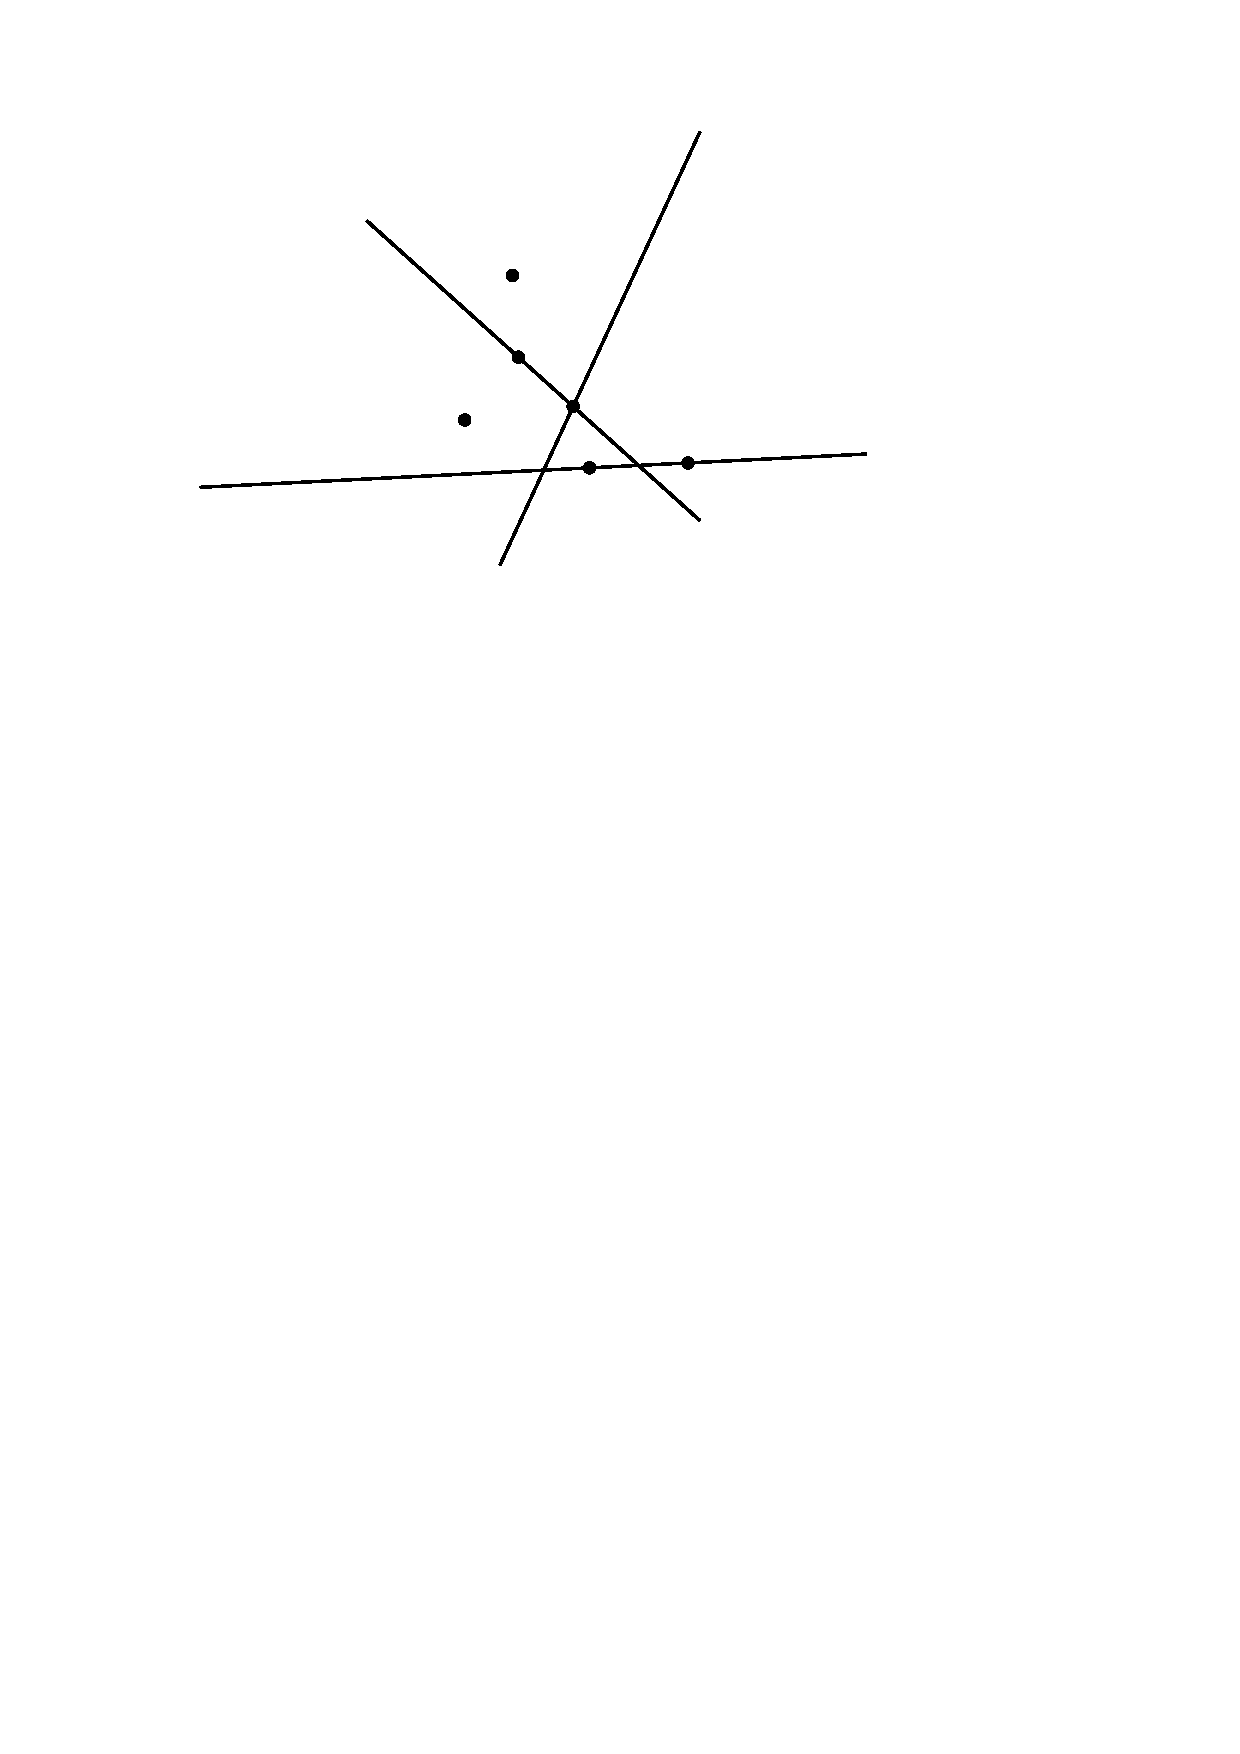
\includegraphics{L1f1.pdf}
\caption{An example of a collection $L$ of lines and $P$ of points. We are interested in the number of \defn{incidences} $I(P,L)$ between points in $P$ and lines in $L$. Here, $I(P,L) = 5$.} \label{fig:IPLexample}
\end{marginfigure}
Suppose we have a collection $L$ of lines in the plane, and $P$ a collection of points in the plane. The set of incidences is $\{(p,\ell): p\in P, \ell\in L, p\in \ell\}$.   Let $I(P,L)$ denote the number of incidences for $P$ and $L$\sidenote{Clearly, $I(P,L) \leq |P| \cdot |L|$, as a subset of $P\times L$.}. Then
\[ 
I(P,L) \leq O ( |P|^{2/3} |L|^{2/3} + |P| + |L| ).
\]
\end{theorem*}
Elekes used this theorem to make progress on the \erdos-Szemer\'edi conjecture by mapping the set $A$ to a collection of points and lines. He showed that if both $|A\cdot A|$ and $|A+A|$ are small, then you find too many incidences.
The Szemer\'edi-Trotter theorem uses the following result:
\begin{lemma*}[Crossing lemma]
Let $G$ be a graph drawn in the plane with crossings. Suppose that $G$ has $m$ edges and $n$ verticies\marginnote{If $m > 3n-6$, then there is at least one crossing, by the result stated at the beginning of the lecture, which comes from Euler's formula. In fact, this is how one proves the crossing lemma.}. If $m\geq 4n$, then there are at least $\frac{m^3}{64 n^2}$ crossings.
\end{lemma*}
From $P$ and $L$, one makes a graph and applies the Crossing Lemma to prove Szemer\'edi-Trotter.




\renewcommand\thesection{\arabic{section}}
\renewcommand\thesubsection{\thesection.\arabic{subsection}}
\setcounter{section}{0}



\clearpage
\newrefsegment
%!TEX root = ../CombinatoricsNotes.tex

 \section{Representing Sets and Sperner Systems.}
 \lect{1}{11}
% \marginnote{Lecture 2: Monday, January 11, 2016. }
\marginnote{We begin our systematic investigation into extremal combinatorics.}
Let's start with some definitions. 
\begin{itemize}[]
\item[Power set:] 
Let $X$ be a finite set with cardinality $|X| = n$. The \defn{power set} is $\P(X)$, the collection of subsets of $X$. $|\P(X)|= 2^n$.
\item[$r$-element subsets:] 
The set $X^{(r)}$ is the collection of all $r$-element subsets of $X$. The cardinality $|X^{(r)}| = {n\choose r}$.
\item[Set system:]
A \defn{set system} $\F \subset \P(X)$ on $X$ is a collection of subsets of $X$. For example, $\F = \{\emptyset, \{1\}, \{1,2\}, \{2,3\},\{3\}\}$ is a set system on $\{1,2,3\}$.
\item[$r$-graph:]
If $\F\subset X^{(r)}$, then we call $\F$ an $r$-graph or \defn{hypergraph}. 2-graphs are just ordinary graphs: $\F\subset X^{(2)}$ can be thought of as a graph with vertex set $X$, edge set $\F$.
\end{itemize}
We'll also frequently use the notation $[n] = \{1,2,\dotsc,n\}$.

\newthought{Now, given a set system} $\{A_1,A_2,\dotsc,A_m\}$, we want to ``reduce'' the sets such that distinct sets remain distinct.
That is, we want to find $S\subset X$ as small as possible such that $\{A_1\cap S, A_2\cap S, \dotsc, A_m\cap S\}$ are all distinct. \marginnote{Note that $S$ acts by deleting elements from our base set $X$.}
Let's start with two sets, $\{A_1,A_2\}$. We want $S$ as small as possible such that $A_1\cap S\neq A_2\cap S$. In this case, we can simply choose $S$ to be a singleton of an element which is in one set but not the other\sidenote{which always exists because $A_1\neq A_2$.}.
If we use our example earlier, $\{\emptyset, \{1\}, \{1,2\}, \{2,3\},\{3\}\}$ on $[3]$, we cannot remove any; $|\P([2])| = 4$ and we have five elements.
If our set system is $\{\emptyset, \{1,2\}, \{2,3\},\{3\}\}$ on $[3]$, then we may remove $1$; that is, $S = \{2,3\}$.
This motivates a question: How small can $S$ be as a function of $m$?
\begin{theorem}
Let $\F = \{A_1,A_2,\dotsc,A_m\}$ be a set system. Then there exists $S$, $|S|\leq m-1$ such that $A_1\cap S$, $A_2\cap S$, \ldots, $A_m\cap S$ are all distinct.
\end{theorem}
\begin{remark}
The bound is tight: the set system $\{\emptyset, \{1\}, \{2\}, \dotsc, \{m-1\}\}$ has the property that if we remove any element, we collapse two sets to the empty set.
\end{remark}
\begin{proof}	
Choose $S$ as small as possible such that $A_1\cap S$, $A_2\cap S$, \ldots, $A_m\cap S$ are all distinct, and assume that $|S| \geq m$.
Let $A_i' = A_i\cap S$. By the minimality of $S$ for every $x\in S$ there exists $i,j\in[m]$ such that $A_i'\setminus \{x\} = A_j'\setminus \{x\}$, with $i\neq j$.

Now, construct a graph  on the vertex set $[m]$ as follows. For each $x\in S$, choose one pair $i$ and $j$ ($i\neq j$) such that $A_i'\setminus \{x\} = A_j'\setminus \{x\}$, and join $i$ and $j$ by an edge\sidenote[][-2cm]{$A_i'\setminus \{x\} = A_j'\setminus \{x\}$ is equivalent to $A_i \symd A_j  =\{x\}$, where the symmetric difference $X\symd Y = (X\cup Y)\setminus (X\cap Y)$.
Because of this, we will make a new edge each time: if $x,y\in S$ yielded the same edge, then $\{x\}=A_i \symd A_j = \{y\} $.}. 
This graph has $m$ verticies and $|S|\geq m$ edges, so it contains a cycle\sidenote{Easy to see by picture; draw $m-1$ edges on $m$ vertices, and then if you don't have a cycle yet, you have a line, and no matter how you place the last edge, you get a cycle.}. Without loss of generality, assume there is a cycle on verticies $1,2,\dotsc,k$ in order. Then there exists distinct $x_1,x_2,\dotsc,x_k\in S$ such that $A_1\symd A_2 = \{x_1\}$, $A_2\symd A_3 = \{x_2\}$, \ldots, $A_{k-1}\symd A_k = \{x_{k-1}\}$, and $A_k \symd A_1 = \{x_k\}$. 

We can take the symmetric difference of all of them:
\[
\emptyset = (A_1\symd A_2) \symd (A_2 \symd A_3) \symd \dotsm \symd (A_k \symd A_1) = \{x_1,x_2,\dotsc, x_k\}
\]
\marginnote{Note the symmetric difference is commutative and associative.}
On the left, we have two of each set, so we can regroup and commute to obtain the empty set, using $A\symd A = \emptyset$. On the right, we have the symmetric difference of distinct singletons, which is just the union. This is a contradiction, so our minimal $S$ must have $|S|\leq m-1$.
\end{proof}
Before we continue finding ways to represent sets, we'll need some graph theoretic tools. First, some definitions.
% \begin{definition}
\begin{itemize}[]
	\item[Bipartite:]  
A graph $G$ is \defn{bipartite}[graph!bipartite] with bipartition $(V_1,V_2)$ if every edge of $G$ contains one vertex of $V_1$ and one vertex of $V_2$. 

\item[Matching: ]A collection of edges $M$ of $G$ is a \defn{matching}[graph!matching] of $V_1$ into $V_2$ if for every $v\in V_1$, $M$ contains exactly one edge containing $v$, and for $v\in V_2$, at most one edge. This is illustrated in \cref{fig:bipartite_matching}.

\begin{marginfigure}
\begin{center}
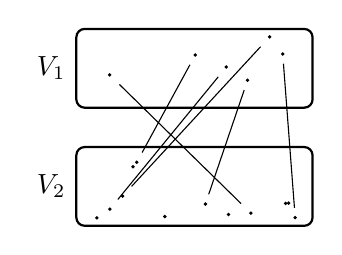
\begin{tikzpicture}[color=black]

\node (rect) at (0,0)[draw,thick,minimum width=3cm, minimum height = 1cm, rounded corners=3pt,label=left:$V_2$]{};

\node (rect2) at (0,1.5)[draw,thick,minimum width=3cm, minimum height = 1cm, rounded corners=3pt,label=left:$V_1$]{};

\pgfmathsetseed{2}
% \def\z{rand}
\foreach \x in {1,...,6}
{
\filldraw (rand*1.4,rand*.4) circle (0.4pt) node(a\x){};
\filldraw (rand*1.4,1.5+rand*.4) circle (0.4pt) node(b\x){};
}

%some extra nodes in the bottom one
\foreach \x in {1,...,6}
{
\filldraw (rand*1.4,rand*.4) circle (0.4pt);
}

\foreach \x in {1,...,6}
{
% \ifthenelse{\x > 1}{\draw[dashed] (a\x) -- (u)}{};
% \foreach \y in {1,...,\x}
% {
\draw (a\x) -- (b\x);
% }
}

\end{tikzpicture}
\end{center}
\caption{Think of elements of $V_1$ as job applicants, and $V_2$ as positions. Then a matching of $V_1$ into $V_2$ is an arrangement so that every job applicant has a position, but some positions could be unfilled.  \label{fig:bipartite_matching}}
\end{marginfigure}


\item[Neighborhood:] For $S\subset V_1$, define the \defn{neighborhood}[graph!neighborhood] $N(S)$ as the set of verticies adjacent to at least one vertex in $S$.
\end{itemize}
The following result\sidenote{\cite{Hallmarriage}} connects these ideas.
\begin{theorem}[Hall's marriage theorem]
Let $G$ be a bipartite graph with bipartition $(V_1,V_2)$. Then $G$ contains a matching of $V_1$ into $V_2$ if and only if 
\begin{equation}	 \label{eq:Hall_condition}
|N(S)| \geq |S| \text{ for every } S\subset V_1. \tag{Hall's condition}
\end{equation}
\end{theorem}
\begin{proof}	
The condition is necessary because you need to have enough verticies available in $N(S)$ for elements of $S$ to match into. We will prove sufficiency by induction on $|V_1|$. The base case is immediate. For the induction step, we will split into two cases.
\begin{enumerate}[{Case }1:]
	\item For every $S\subset V_1$ with $S\neq \emptyset$ and $S\neq V_1$, we have that $|N(S)| > |S|$. 
% \end{enumerate}
In this case, choose  $v\in V_1$; then $v$ has a $w\in V_2$ adjacent to it, because $|N(\{v\})|> |\{v\}|=1$. Apply the induction hypothesis to $G \setminus \{v,w\}$.

We then just need to check Hall's condition on $G' =G \setminus \{v,w\}$. For every $S\subset V_1 \setminus\{v\}$, we have 
\[	
 |N'(S)| \geq |N(S)| -1 \geq |S|,
\]
 where $N'$ is the neighborhood with respect to $G'$. The first inequality holds because we removed at most one neighbor by removing $w$. The second inequality holds from our assumption in this case. Then the induction hypothesis yields a matching on $V_1\setminus \{v\}$ into $V_2\setminus \{w\}$, which we can extend to a matching on $V_1$ into $V_2$ by matching $v$ to $w$.
% \begin{enumerate}[{Case }1:]\setcounter{enumi}{1}
\item There exists $S\subset V_1$ with $S\neq \emptyset$ and $S\neq V_1$, such that $|N(S)| = |S|$. 
% \end{enumerate}
By induction hypothesis,  there exists a matching $M_1$ of $S$ into $N(S)$.

 It remains to find a matching from $V_1\setminus S$ into $V_2 \setminus N(S)$. By induction hypothesis, it is enough to show that for every $T\subset V_1\setminus S$, we have
\[
 |N(T)\cap (V_2 \setminus N(S))| \geq |T|.
\]
 \marginnote{Here's the trick.}Since $S\cup T\subset V_1$, by assumption, we have Hall's condition
\[
 |N(S\cup T)|\geq |S\cup T| = |S| + |T|.
\]

 We know $N(S\cup T) = N(S) \cup N(T) = N(S) \cup (N(T)\setminus N(S))$. So $|N(S\cup T)| = |N(S)| + |N(T)\setminus N(S)| $. So Hall's condition becomes
\[
 |N(T)\setminus N(S)| \geq |T|
\]
 as desired.\qedhere
 \end{enumerate}
\end{proof}


Let's employ Hall's theorem to represent sets. Let 
\[
 \F = \{A_1,A_2,\dotsc,A_m\}
 \] be a set system.
% \begin{definition}
A \defn{system of distinct representatives} for $\F$ is a collection $\{x_1,\dotsc,x_m\}$ of elements such that $x_1,\dotsc, x_m$ are pairwise distinct, and $x_i \in A_i$ for $i\in[m]$.
% \end{definition}
Given $\F$, one can consider the bipartite graph $G$ with bipartition $(V_1,V_2)$ such that $V_1 = \F$ and $V_2= \bigcup_{i\in[m]} A_i$. We join $A_i$ to $x$ iff $x\in A_i$.
Then a system of distinct representatives for $\F$ is exactly a matching on $G$ from $V_1$ into $V_2$. Hall's theorem then immediately implies the following result.
\begin{corollary}
A set system $\F = \{A_1,\dotsc,A_m\}$ has a system of distinct representatives if and only if for every $\F'\subset \F$, 
\[
|\F'| \leq \left|\bigcup_{A\in \F'}A\right|.
\]
\end{corollary}
\newthought{Given a set $X$}, there is a natural bipartite graph and matching which will prove useful.
\begin{corollary} \label{cor:Xr_matching_exists}
Let $X$ be a set with $|X|=n$. Let $G$ be a bipartite graph with bipartition $(X^{(r)}, X^{(r-1)})$ such that $A\in X^{(r)}$ is adjacent to $B \in X^{(r-1)}$ if $B\subset A$. Then if  $r> n/2$, the graph $G$ has a matching of $X^{(r)}$ into $X^{(r-1)}$.
\begin{marginfigure}
\begin{center}
 \begin{tikzcd}[column sep=tiny]
X^{(3)}  & &\{1,2,3\}  \\
X^{(2)} &\{1,2\} \arrow[dash,green]{d}  \arrow[dash]{rd}& \{1,3\} \arrow[dash]{ld}\arrow[dash]{d} \arrow[dash,green]{rd} & \arrow[dash,green]{ld} \arrow[dash]{d}\{2,3\} \\
X^{(1)} & \{1\}  & \{2\} &\{3\} \\
X^{(0)} & & \emptyset
\end{tikzcd}
\end{center}
\caption{Example of the graph relation on $G= (X^{(2)}, X^{(3)})$, with a matching highlighted in green.}
\end{marginfigure}
\end{corollary}
\begin{remark}
This corollory implicitly shows ${n \choose r} \leq {n \choose r-1}$ if $r> n/2$.
\end{remark}
\begin{proof}	
It suffices to check \ref{eq:Hall_condition}. For every $\A\subset X^{(r)}$, we want $|N(\A)| \geq |\A|$. Label
\[
\B:= N(\A) = \{B\in X^{(r-1)}: B\subset A, \text{ for some }A\in \A\}.
\]
Every element of $X^{(r)}$ is incident to $r$ edges of $G$\sidenote{Each edge corresponds to taking an element away from the set.}. So we have $|\A|r$ edges leaving $\A$, ending in $\B$.
Every element of $X^{(r-1)}$ is incident to $n-r+1$ edges of $G$, which can be seen by the fact that there are $n-(r-1)$ possible elements to add to a set $B\in X^{(r-1)}$ to obtain a superset in $X^{(r)}$. So we have at most $|\B|(n-r+1)$ edges leaving $\B$, ending in $\A$\sidenote{Since not every edge leaving $\B$ needs to reach something in $\A$ (it could reach something in $X^{(r)} \setminus \A$), it is only ``at most.''}.
So $|\A|r \leq |\B|(n-r+1)$. But by assumption $r \geq (n-r+1)$, so $|\B| \geq |\A|$ as desired.
\end{proof}

\lect{1}{13}
% \marginnote{Lecture 3: Wednesday, January 13, 2016.}

Recall that $\F\subset \P(X)$ is a \emph{Sperner system} if for all $A,B\in \F$, if $A\leq B$, then $A=B$.
We wish to find $\max |\F|$ such that $\F$ is a Sperner system, as a function $|X| = n$. Note that $X^{(r)}$ is always Sperner, and $|X^{(r)}| = {|X| \choose r}$, which is maximized when $r = \floor{n/2}$.
\begin{theorem}[\cite{sperner1928}] \label{thm:sperner}
If $\F\subset \P(X)$ is Sperner, then $|\F| \leq {n \choose \floor{n/2}}$, where $n=|X|$.
\end{theorem}
\begin{proof}	
\marginnote{A Sperner system is a system of sets such that no two are comparable. A dual notion is a system of sets such that all are comparable. }
An ordered collection $(A_1,A_2,\dotsc, A_k)$ of sets  in $\P(X)$  is a \defn{chain} if $A_1\subsetneqq A_2 \subsetneqq A_3 \subsetneqq\dotsm \subsetneqq A_k$. 
\begin{marginfigure}
\begin{center}
 \begin{tikzcd}[column sep=tiny]
X^{(3)}  & &\{1,2,3\} \arrow[dash]{d}\arrow[dash]{rd}\arrow[dash,green]{ld} \\
X^{(2)} &\{1,2\} \arrow[dash,green]{d}  \arrow[dash]{rd}& \{1,3\} \arrow[dash]{ld}\arrow[dash]{d} \arrow[dash,blue]{rd} & \arrow[dash,red]{ld} \arrow[dash]{d}\{2,3\} \\
\mathbf{X^{(1)}} & \mathbf{\{1\}} \arrow[dash,green]{rd} & \mathbf{\{2\}} \arrow[dash]{d}&\mathbf{\{3\}}\arrow[dash]{ld} \\
X^{(0)} & & \emptyset
\end{tikzcd}
\end{center}
\caption{Consider $X^{(1)}$, a natural maximal Sperner system. Note that each element of $X^{(1)}$ can form a distinct chain, such as $\emptyset \subsetneqq \{1\} \subsetneqq \{1,2\} \subsetneqq \{1,2,3\}$.}\label{fig:Sperner_chains}
\end{marginfigure}
It is enough to show that $\P(X)$ can be partitioned into ${n \choose \floor{n/2}}$ chains. Indeed, every Sperner system can contain $\leq 1$ element from each chain in the partition; see \cref{fig:Sperner_chains} for an example.
Better yet, we partition $\P(X)$ into chains such that every chain contains an element of $X^{(\floor{n/2})}$. 

Let's begin by partitioning all subsets of $X$ of size $\geq \floor{n/2}$.
We will first do this inductively starting from $X^{(\floor{n/2})}$, and extending the partition to $X^{(\floor{n/2})}\cup X^{(\floor{n/2}+1)}\cup\dotsm \cup X^{(k)}$ to $X^{(k+1)}$ using the matching obtained in \cref{cor:Xr_matching_exists} from $X^{(k)}$ to $X^{(k+1)}$ by adding each element of $X^{(k+1)}$ to the chain of the set it's matched to. Note that are chains are not maximal; some (all but one) truncate before they reach the top, $X^{(n)}$.
Then we can extend the partition to sets of size $< \floor{n/2}$ by symmetry.
\end{proof}
\begin{remark}
This proof is instructive and provides the useful technique of partitioning into chains. But we can prove stronger results with slicker proofs.
\end{remark}
Suppose $k< n/2$ and we want to find the maximum size Sperner system such that every set in the system has size $\leq k$.
As one may guess, the maximum size will be $|X^{(k)}| = {n\choose k}$. To show this, we'll use the following result.
\begin{theorem}[Lubell, Meshalkin, Yamamoto, Boll\'obas, and possibly others, A.K.A. the LYM inequality] \marginnote{\cite{LUBELL_LYM,Meshalkin_LYM,yamamoto1954_LYM,Bollab_LYM}}
\label{thm:LYM_inequality}
Let $\F\subset \P(X)$, $|X|=n$ be a Sperner system.
Let $\F_k = \F\cap X^{(k)}$ be the set of $k$ element sets in $\F$, and let $f_k = |\F_k|$. Then
\begin{equation}	\tag{LYM} 
\label{eq:LYM}
\sum_{k=0}^n \frac{f_k}{{n\choose k}} \leq 1.
\end{equation}
\end{theorem}
\begin{remark}
We have
\[
1 \geq \sum_{k=0}^n \frac{f_k}{{n\choose k}} \geq \sum_{k=0}^n \frac{f_k}{{n\choose \floor{n/2}}},
\]
thus
\[
{n\choose \floor{n/2}} \geq \sum_{k=0}^n f_k = |\F|
\]
which is Sperner's theorem.
\end{remark}
\begin{proof} Let's assume $X=[n]$ for convenience.
Consider all maximum chains in $\P(X)$ and count how many chains an element of $\F$ belongs to. Each of the maximal chains is of the form $\emptyset = A_0$, $A_1$, \ldots, $A_n = X = [n]$, and $|A_i| = i$. So each maximal chain corresponds to an ordering $a_1,a_2,\dotsc,a_n$ of $[n]$, where $\{a_i\} = A_i \setminus A_{i-1}$, is the element you add to $A_i$ to get the next set in the chain.

Thus, there are $n!$ maximal chains (the number of re-orderings of $[n]$). Consider
$F \in X^{(k)}$.
How many  maximal chains is $F$ in? If $k=0,n$, $F$ is in every chain, so $n!$. If $k=1$, then $F$ is in $(n-1)!$ chains. If $k=2$, then $2!(n-2)!$. In general, $F$ is in $k!(n-k)!$ maximal chains\sidenote{We choose $k$ to get to the set, then $(n-k)$ to finish the chain.} Each maximal chain contains $\leq 1$ element of $\F$. The total number of elements of $\F$ in all maximum chains is
\[
 \sum_{k=0}^n f_k k!(n-k)!\leq n!
\]
Dividing by $n!$, we obtain the LYM inequality.
\end{proof}
\begin{remark}
Let's consider an alternate proof. Let $C$ be a uniformly randomly chosen maximal chain, and consider the expectation value of the number of elements of $C\cap \F$. Of course, there is at most 1 element, since $\F$ is a Sperner system. On the other hand,
\begin{align*}	
\E ( | C\cap \F|) &=\sum_{k=0}^n \E( | C \cap \F_k|) = \sum_{k=0}^n f_k \cdot (\text{probability that a set of size $k$ is in $C$})\\
 &=  \sum_{k=0}^n f_k \cdot \frac{1}{(\text{number of sets of size $k$)}} = \sum_{k=0}^n \frac{f_k}{{n \choose k}} \leq 1.
\end{align*}
\end{remark}


When does equality hold in LYM? Certainly when $\F= X^{(r)}$ for any $r$. We'd like to show this condition is necessary as well, but to do so, we'll first prove a more refined inequality in which equality is easier to check. Then we'll use this to show sufficiency for equality in the LYM inequality.

\begin{theorem}[Local LYM inequality] \label{thm:local_LYM}
Let $\A\subset X^{(r)}$, and $|X|=n$. Define
$\partial \A \subset X^{(r-1)}$
the \defn{shadow} of $A$ by
\[
\partial \A := \{B\in X^{(r-1)}: B\supseteq A \text{ for some }A\in \A \}.
\]
Then
\begin{equation}	\label{eq:local_LYM} \tag{Local LYM}
\frac{|\partial \A|}{{n\choose r-1}} \geq \frac{|\A|}{{n \choose r}}
\end{equation}
or equivalently,
\[
 r| \A| \leq |\partial \A| (n-r+1).
\]
Moreover, equality holds if and only if $\A= \emptyset$ or $\A=  X^{(r)}$.
\end{theorem}
\begin{proof}	
\[
 r|\A| = | \{ (B,A): B\in \partial A, \, A\in \A, \, B\subset A\}| \leq |\partial A| (n-r+1)
 \] as seen in \cref{cor:Xr_matching_exists}.
If equality holds, then $\A$ contains all supersets in $X^{(r)}$ of all sets in $\partial A$. 


\begin{marginfigure}
\begin{center}
\begin{tikzcd}[column sep=tiny]
\A & \{x_1,\dotsc,x_r\} \arrow[dash]{d} \arrow[dash]{rd} & \arrow[dash]{ld} \\
\partial \A & \{x_2,\dotsc,x_n\} & \{x_1,x_2,\dotsc,x_n\}
\end{tikzcd}
\end{center}
\caption{If $\A$ contains all supersets in the $X^{(r)}$ layer of sets in the shadow $\partial \A$, then as long as $\A\neq \emptyset$, it must contain every set; here, for example, $\A$ has to include the endpoint of the edge leaving the bottom left vertex. }
\end{marginfigure}

Consider the graph as in \cref{cor:Xr_matching_exists}:  there are no edges from $A\cup \partial A$ to the remaining verticies, so since $G$ is connected\sidenote{as is easy to check},  we have equality in \eqref{eq:local_LYM}.
\end{proof}

\begin{theorem}
The equality in the LYM inequality \eqref{eq:LYM} holds iff $\F = X^{(r)}$ for some $r$.
\end{theorem}
\begin{proof}	
Inductively define $G_n = \F_n$, and for $k < n$, $G_k  = \partial G_{k+1} \cup \F_k$. \marginnote{$G_k$ is the set of all $k$-element sets which are subsets of sets in $\F$.}

Let $\phi_k = \frac{f_k}{{n \choose k}}$ be the proportion of sets of $\F$ in $X^{(k)}$. Similarly, set $\gamma_k = \frac{|G_k|}{{n\choose k}}$. By the local LYM,
\[
\frac{|\partial G_{k+1}|}{{n\choose k}} \geq \frac{|G_{k+1}|}{{n\choose k+1}} = \gamma_{k+1}
\]
So,
\[
\gamma_k = \frac{|\partial G_{k+1} \cup \F_k|}{{n\choose k}} = \frac{|\partial G_{k+1}|}{{n\choose k}} + \frac{|\F_k|}{{n\choose k}} \geq  \gamma_{k+1} + \phi_k
\]
where we are using that $\F$ is Sperner, so that $\partial G_{k+1}$ is disjoint from $\F_k$. Thus, we have $\gamma_k \geq \gamma_{k+1} + \phi_k$, with equality iff $\gamma_{k+1} = 1$ or $\gamma_{k+1} = 0$. \marginnote{Since that is when we have equality in \cref{eq:local_LYM}.}

Note $\gamma_n = \phi_n$. Then
\begin{gather*}	
\gamma_{n-1} \geq \gamma_n + \phi_{n-1} = \phi_n + \phi_{n-1}\\
\gamma_{n-2} \geq \gamma_{n-1} + \phi_{n-2} = \phi_n + \phi_{n-1} + \phi_{n-2}\\
\text{etc.}\\
\gamma_k \geq \phi_n + \phi_{n-1} + \dotsm + \phi_k.
\end{gather*}
Hence, $1 \geq \gamma_0 \geq \phi_n + \phi_{n-1} + \dotsb + \phi_0$. This is the LYM inequality. But equality holds if $\gamma_k = \gamma_{k+1} +\phi_k$ for each $k$, i.e. $\gamma_{k+1} = 1$ or $\gamma_{k+1} = 0$ for each $k$. Assuming we have equality, we use that $\gamma_k$ is non-increasing with $k$, so there must exist $k_0$ such that $\gamma_{k_0} = 1$, and $\gamma_{k_0+1} = 0$ (writing $\gamma_{n+1} = 0$). Thus, there are no sets in $\F$ of size at least $k+1$. In other words, $G_{k+1} = \emptyset$, and $G_k = \F_k = X^{(k)}$. But then we must have $\F  = X^{(k)}$ as desired, since $\F$ may not have any super sets or subsets of $X^{(k)}$, i.e., any other set in $\P(X)$.
\end{proof}
\begin{remark}
The matchings with $X^{(r)}$ and $X^{(r-1)}$ are the essential objects here in proving the local LYM, and hence LYM and its equality.
\end{remark}
\begin{exercise}
Prove Sperner's theorem using the original way: partitioning into ${n\choose \floor{n/2}}$ chains by induction on $n$ instead of Hall's theorem.
\marginnote{This is \cref{thm:sym_part}.}
\end{exercise}


\begin{fullwidth}
\printbibliography[segment=\therefsegment,heading=subbibliography]
\end{fullwidth}


\clearpage
\newrefsegment
%!TEX root = ../CombinatoricsNotes.tex

\section{The Littlewood-Offord problem}
\lect{1}{18}
% \marginnote{Lecture 4: Monday, January 18, 2014.}

\begin{problem}[\cite{LO1943}]
Given $(z_1,\dotsc,z_n)$ complex numbers, with $|z_i| \geq 1$. Consider the $2^n$ possible sums formed by the $z_i$'s. How many sums can have pairwise distances less than 1 from each other? If $z_1 = z_2 = \dotsc =z_n=1$, then we get ${n \choose \floor{n/2}}$ equal sums.

Given $(z_1,\dotsc,z_n)$, and subset of indicies $A\subset [n]$, let $Z_A = \sum_{i\in A} z_i$, where we define  $Z_\emptyset = 0$ and $Z_{\{i\}} = z_i$. We say $\F \subset \P([n])$ is \defn{Littlewood-Offord}[Littlewood-Offord!sets of numbers] (LO) with respect to $(z_1,\dotsc,z_n)$ if $|Z_A- Z_B| < 1$ for all $A,B \in \F$. In this notation, we are looking for the largest collection $\F$ such that $\F$ is LO with respect to $(z_1,\dotsc,z_n)$.
\end{problem}

\begin{conjecture*}
If $(z_1,\dotsc,z_n) \in \C^n$ with $|z_i|\geq 1$, and $\F$ is LO with respect to $(z_1,\dotsc,z_n)$, then $|\F| \leq {n \choose \floor{n/2}}$.
\end{conjecture*}
\begin{remark}
Littlewood and Offord were not combinatorialists; instead they were interested in studying the roots of random polynomials.
\end{remark}

\begin{theorem}[\cite{erdos1945}]
If $x_1,\dotsc,x_n$ are real, $|x_i| \geq 1$ for every $i$, and $\F$ is LO with respect to $(x_1,\dotsc,x_n)$, then $|\F| \leq { n\choose \floor{n/2}}$.
\end{theorem}
\begin{proof}	
We'll change notation to $X_A$ instead of $Z_A$ for this real case. If $x_1,\dotsc,x_n \geq 1$, then $\F$ is Sperner. Suppose $A\subsetneq B$; then
\[
|X_A - X_B| = X_B - X_A = X_{B\setminus A} \geq |B-A| \geq 1. \qquad \checkmark
\]

The general problem for reals can be reduced to this case of $x_i>0$ as follows.
Suppose that $\F$ is LO with respect to $(x_1,\dotsc,x_n)$. Then we will construct a family $\F'$ which is LO with respect to \\$(x_1,\dotsc, x_{i-1},-x_i, x_{i+1}, \dotsc, x_n)$ with $|\F'| = |\F|$. This will suffice to prove the theorem.

Let $\F' = \{ A \symd \{i\}: A\in \F\}$\sidenote[][]{We remove $i$ if it's there, and add it otherwise.}. Clearly $|\F'| = |\F|$. We've reduced all sums by $x_i$, as shown by the following. If $i \in A$, then $X'_{A \symd \{i\}} = \left(\sum_{j\in A} x_j \right)-x_i$. if $i \not \in B$, then $X'_{B \symd \{i\}} = \left( \sum_{j\in B} x_j \right) - x_i$.
Hence, all sums are still within $1$ of each other, completing the proof.
\end{proof}



\begin{definition}
A chain $A_1 \subset A_2 \subset \dotsc \subset A_k$ in $\P([n])$ is \defn{symmetric}[symmetric!chain] if $|A_{i+1}| = |A_i| +1$ for $i=1,\dotsc,k-1$. Additionally, we require $|A_1| + |A_k| = n$. 
\end{definition}
Note that in particular, a symmetric chain  intersects $[n]^{(\floor{n/2})}$. An example of symmetric chains is shown in \cref{fig:sym_chains}.
\begin{figure}[ht]
\begin{center}
 \begin{tikzcd}[column sep=tiny]
{[3]}^{(3)}  & &\{1,2,3\}\arrow[green,dash]{ld} \\
{[3]}^{(2)} &\{1,2\} \arrow[dash,green]{d}& \{1,3\}  \arrow[dash,blue]{rd} & \arrow[dash,red]{ld} \{2,3\} \\
\mathbf{[3]^{(1)}} & \mathbf{\{1\}} \arrow[dash,green]{rd} & \mathbf{\{2\}}&\mathbf{\{3\}}\\
{[3]}^{(0)} & & \emptyset
\end{tikzcd}
 \begin{tikzcd}[column sep=tiny]
&\{1,2,3\}\arrow[red,dash]{rd} \\
\{1,2\} \arrow[dash,green]{d}& \{1,3\}  \arrow[dash,blue]{rd} & \arrow[dash,red]{ld} \{2,3\} \\
 \mathbf{\{1\}} \arrow[dash,green]{rd} & \mathbf{\{2\}}&\mathbf{\{3\}}\\
 & \emptyset
\end{tikzcd}
\end{center}
\caption{\textit{Left:} We draw our favorite $\P([n])$, partioned into symmetric chains, which thus each intersect $[n]^{(\floor{n/2})}$. \textit{Right:} A partition of $\P([n])$ into chains which intersect $[n]^{(\floor{n/2})}$, which we could obtain from the proof of \cref{thm:sperner}. But these chains are not symmetric.} \label{fig:sym_chains} 
\end{figure}

Our previous method, when proving Sperner's theorem, didn't actually guarantee symmetric chains; see \cref{fig:sym_chains}. We will do this now, which provides a new proof of Sperner's theorem.

\pagebreak
\begin{theorem} \label{thm:sym_part}
$\P([n])$ can be partitioned into symmetric chains.
\end{theorem}
\begin{proof}[Proof by induction on $n$.]
 The base case $n=1$ is immediate.
Induction step: Let $C_1,C_2,\dotsc,C_L$ be symmetric chains forming a partition of $\P{[n-1]}$. Consider $C_i = (A_1,A_2,\dotsc,A_k)$. Form 
\begin{align*}	
 C_i' &= (A_1,A_2,\dotsc,A_k,A_k\cup \{n\})\\
 C_i'' &= (A_1 \cup \{n\}, A_2 \cup \{n\}, \dotsc, A_{k-1} \cup \{n\}).
 \end{align*} 
 % \improvement{Add picture of $n=3$ of $C_i'$ and $C_i''$.}
 \begin{figure}
 \begin{center}
 \begin{tikzcd}[column sep=tiny]
% {[n]}^{(3)}  & &\{1,2,3\}\arrow[green,dash]{ld} \\
\phantom{{[n]}^{(3)}}& & \\
{[2]}^{(2)} &\{1,2\} \arrow[dash,OliveGreen]{d}&  \\
\mathbf{[2]^{(1)}} & \mathbf{\{1\}} \arrow[dash,OliveGreen]{rd} & \mathbf{\{2\}}&\\
{[2]}^{(0)} & & \emptyset
\end{tikzcd}\hfill
\begin{tikzcd}[column sep=tiny]
{[3]}^{(3)}  & &\{1,2,3\}\arrow[DarkGreen,dash]{ld} \\
{[3]}^{(2)} &\{1,2\} \arrow[dash,DarkGreen]{d}& \{1,3\}  \arrow[dash,LightGreen]{rd} & \arrow[dash,red]{ld} \{2,3\} \\
\mathbf{[3]^{(1)}} & \mathbf{\{1\}} \arrow[dash,DarkGreen]{rd} & \mathbf{\{2\}}&\mathbf{\{3\}}\\
{[3]}^{(0)} & & \emptyset
\end{tikzcd}
\end{center}
\caption{An illustration of the induction step, from $n=2$ on the left to $n=3$ on the right. On the left,  two chains: $C_1 = (\emptyset, \{1\}, \{1,2\})$ in green, and $C_2 = (\{2\})$.
We create $C_1' = (\emptyset, \{1\},\{1,2\},\{1,2,3\})$ in dark green, and $C_1'' = (\{3\}, \{1,3\})$ in light green. We also create $C_2' = (\{2\},\{2,3\})$ in red, and $C_2'' = ()$, an empty chain.%
}%
 \end{figure}
We can easily see that given that $C_i$ was a symmetric chain on $\P([n-1])$, we have $C_i'$ and $C_i''$ are both symmetric chains on $\P([n])$. Moreover, 
\[
\{C_1', \dotsc, C_L'\}\cup \{C_1'', \dotsc, C_L''\}
\]
form a partition of $\P([n])$, as follows:  For any set $A\in \P([n])$, if $n\not \in A$, then $A\in C_i$ for some $i$, and hence $A\in C_i'$. If $n\in A$, then $A\setminus \{n\} \in C_i = (A_1,A_2,\dotsc,A_k)$ for some $i$, so $A = A_j$ for some $j$. If $j=k$, then $A\in C_i'$, otherwise $A\in C_i''$. In any case, if $A\in \P([n])$, $A$ is in one of these chains. Finally, $A$ cannot be in two chains, otherwise we have that $\{C_i\}$ was not a partition of $\P([n-1])$.
\end{proof}

Any partition of $\P([n])$ symmetric chains has ${n\choose \floor{n/2}}$ sets, because each chain must intersect with one point in $[n]^{(\floor{n/2})}$.
In the proof, we took a partition into ${n-1 \choose \floor{(n-1)/2}}$ chains, and seem to have created $2 {n-1 \choose \floor{(n-1)/2}} \neq {n\choose \floor{n/2}}$ chains. The catch is that $C_i''$ is an empty chain if $k=1$.


\newthought{Let us count} the sizes of symmetric chains. Suppose $C_1,\dotsc,C_L$ is a partition of $\P([n])$ into symmetric chains, where $L = {n\choose \floor{n/2}}$. How many chains are there of length $r=n+1$ in the partition? Exactly one, the chain which contains the empty set and must therefore contain the set of $n$ elements.

What about $r=n$? Zero.

What about $r= n-1$? $n-1$ chains, because it must start the collection of 1 element sets and go to the collection of $n-1$ element sets. There are $n$ 1-element sets, but one is already in the maximal chain, so we are left with $n-1$.

What about $r= (n+1)-2i$? These are the symmetric chains which start at the $i$th level $[n]^{(i)}$ and go to the $n-i$th level $[n]^{(n-i)}$. The result is ${n\choose i} - {n\choose i-1}$. That is because there are ${n\choose i}$ elements in $[n]^{(i)}$, but ${n\choose i-1}$ of them are part of longer chains, the number of which is the number of elements in the level $[n]^{(i-1)}$.

Let us formulate analogues of these ideas to solve the Littlewood-Offord problem in $\R^d$.
\begin{theorem}[\cite{KLEITMAN1970}] \label{thm:kleit70}
Let $(x_1,\dotsc,x_n)$ be vectors in $\R^d$, with $\|x_i\| \geq 1$. As before, define for $A\subset [n]$, $X_A = \sum_{i\in A} x_i$, and say that $\F\subset \P([n])$ is \defn{LO}[Littlewood-Offord!sets of vectors] with respect to $(x_1,\dotsc,x_n)$ if for each $A,B\in \F$, we have $\|X_A - X_B\| < 1$.
Let $\F$ be LO with respect to $(x_1,\dotsc,x_n)$. Then $|\F| \leq { n\choose \floor{n/2}}$.
\end{theorem}
\begin{proof}	
We will say $\Cset\subset \P([n])$ is \defn{sparse}[sparse!set of indicies of vectors] (with respect to $(x_1,\dotsc,x_n)$) if $\|X_A-X_B\| > 1$ for all $A,B\in \Cset$ with $A\neq B$.x
It is enough to show that $\P([n])$ can be partitioned into ${n\choose \floor{n/2}}$ sparse sets\sidenote{A LO family may only contain one element of each sparse set.}. 

We say that a partition $C_1,\dotsc,C_L$ of $\P([n])$ is \defn{symmetric}[symmetric!partition] if it contains exactly ${n\choose i} - {n\choose i-1}$ ``chains'' of order $(n+1)-2i$ for $i=0,1,\dotsc,\floor{n/2}$, and no chains with sizes not congruent to $n+1 \mod 2$. \marginnote{Here, ``chain'' simply means a set $C_i$ for some $i\in [L]$.}  In particular, $L= {n\choose \floor{n/2}}$.

We will show that $\P[n]$ has a symmetric partition into sparse sets. Then we will have found $L = {n\choose \floor{n/2}}$ sparse sets, completing the proof.
Let's proceed by induction on $n$. For $n=1$, we have $X_\emptyset = 0$, and $X_{\{1\}} = x_1$. Then $\{\emptyset, \{1\}\}$ is sparse if $\|X_\emptyset - X_{\{1\}}\| > 1$, which holds because $\|x_1\| > 1$.
Induction step: Let $C_1,C_2,\dotsc, C_L$ be a symmetric partition of $\P([n-1])$ into sets sparse with respect to $(x_1,\dotsc,x_{n-1})$. 

Let $C_i = \{A_1,\dotsc,A_k\}$. We'd like to form sparse sets
\begin{align*}	
C_i' &= \{A_1,A_2,\dotsc,A_k,A_k \cup \{n\}\}\\
C_i'' &= \{A_1\cup \{n\}, A_2\cup\{n\},\dotsc,A_{k-1}\cup \{n\}\}.
\end{align*}
Our sets $A_1,\dotsc,A_k$ do not have an ordering this time, and we may choose any set to be $A_k$. We will have to use this freedom; consider translating the sums in some chain $C_i = (A_1,\dotsc,A_k)$ by adding the vector $x_n$. We want $C_i'$ to be sparse, but then we need $X_{A_k\cup\{n\}}$ far from each $X_{A_j}$, which does not always need to happen, as illustrated in \cref{fig:LO_proof_prob}.
\begin{marginfigure}[-3cm]
%!TEX root = ../Combinatorics.tex

\newcommand{\makearrow}[2]{
    \begin{scope}
    \coordinate (A) at (#1);
    \coordinate (B) at ([xshift=+120pt,yshift=+60pt]A);
    \draw (A) edge[->] (B);
\end{scope}
}

\newdimen\XCoord
\newdimen\YCoord

\newcommand*{\ExtractCoordinate}[1]{\path (#1); \pgfgetlastxy{\XCoord}{\YCoord};}%
\newcommand*{\LabelCurrentCoordinate}[2]{\fill [#1] ($(\XCoord,\YCoord)$) circle (2pt) node [right] {#2}}%

\pgfmathsetseed{3}

\begin{center}
\begin{tikzpicture}[scale=.25]
\def\scale{.1};
\def\x{2};
\def\y{5};

\coordinate (A) at (\x,\y);
\coordinate (B) at ([xshift=+120pt,yshift=+60pt]A);
\draw (A) edge[->,Red] node[auto=right, pos=-0.1]{{\tiny $X_{A_k}$}} node[ auto=right, near end]{{\tiny $X_{A_k\cup\{n\}}$}} (B);

\coordinate (C) at ($ (A) + (4,4) $);
\coordinate (D) at ([xshift=+120pt,yshift=+60pt]C);

\draw (C) edge[->,Blue] node[auto, near start]{{\tiny $X_{A_1}$}} node[ auto=right, near end]{{\tiny $X_{A_1\cup\{n\}}$}} (D);



\dimline[label style={above=0.5ex},extension start length=.24,extension end length=.24]{($ (A) + .24*(-4,4) $)}{($ (C) + .24*(-4,4) $)}{{\tiny $>1$}};

\coordinate (new) at ($ (C) - (B) $);

\ExtractCoordinate{$(new)$};

\coordinate (newer) at ($(\YCoord,-\XCoord)$);
%(\YCord, -\XCord)


\dimline[label style={ above=.2ex,right, rotate=90},extension start length=-.6,extension end length=-.6]{($ (B) + 3*(newer) $)}{($ (C) + 3*(newer) $)}{{\tiny $<1$}};


% \end{scope}

 % \begin{scope}[scale=\scale]
    % \coordinate (C) at $(\x + 10, \y)$;
    % \coordinate (D) at ([xshift=+120pt,yshift=+60pt]C);
    % \draw (C) edge[->] (D);
% \end{scope}

  \foreach \x in {1,2,...,5}{
    \makearrow{rand*5+4,rand*5-2.5}{\scale};}

\makearrow{3,12}{\scale};
\end{tikzpicture}
\end{center}

% 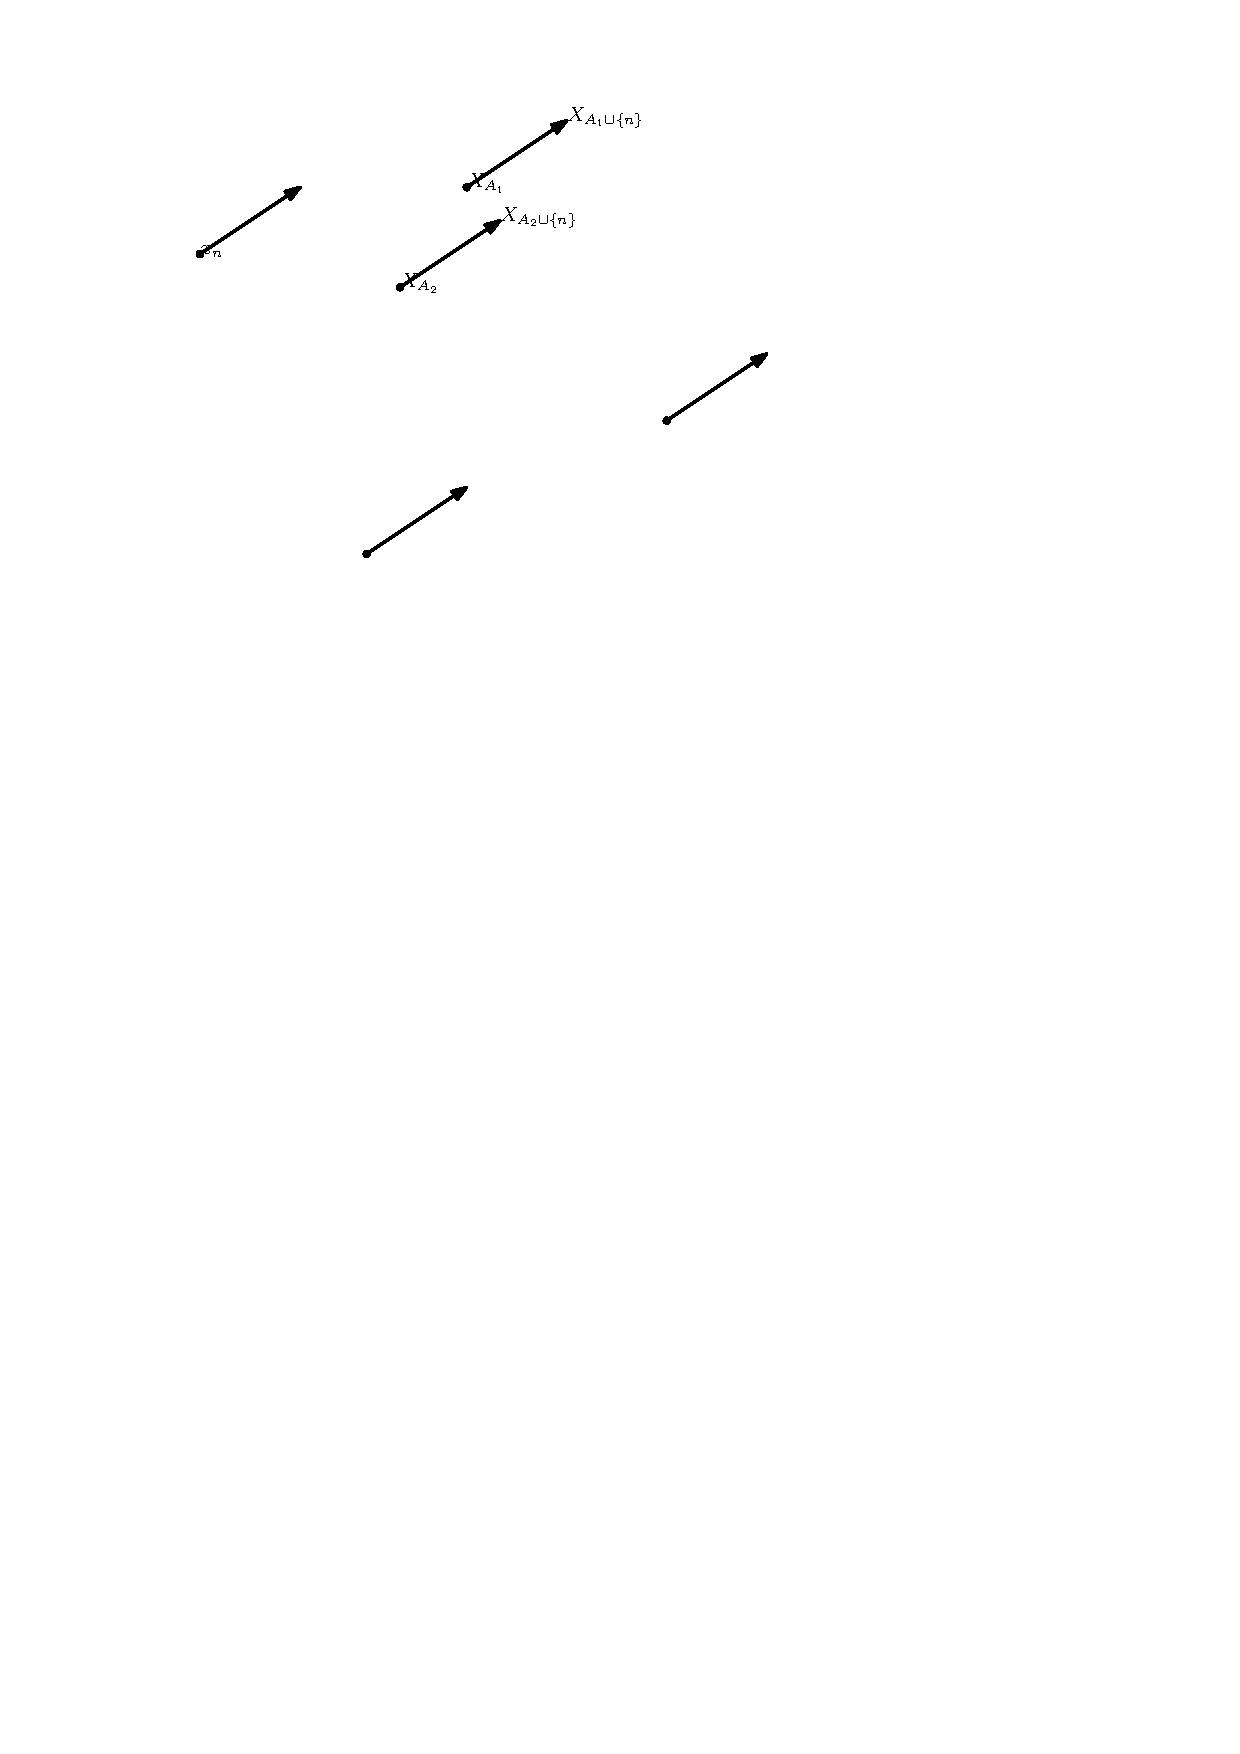
\includegraphics[scale=.5]{graphics/LOproof.pdf}
\caption{With the choice of $A_k$ shown here, we have that $X_{A_k \cup \{n\}} = X_A + x_n$ (in red) is near to $X_{A_1}$ (in blue), so $C_i'$ is not a sparse chain, even though $C_i$ is a sparse chain (all the start points of the arrows are far from each other).} \label{fig:LO_proof_prob}

\end{marginfigure}
% \improvement{Draw better figure, show that the distance is less than 1 in that one spot.}
Assume WLOG that $x_n = (\alpha,0,0,\dotsc,0)$ only has non-zero first coordinate with $\alpha>0$. Let $p(v)$ denote the first coordinate of $v$. Then $p$ is a linear function, and $p(v) \leq \|v\|$ for each $v$. 

Let $A_k$ in the construction above be chosen so that $p(X_{A_k})\geq p(X_{A_j})$ for each $j$\sidenote{So we are choosing $A_k$ to be the furthest in the direction $x_n$. Then if we add $x_n$, we are only moving it further away from the others, so the conflict in \cref{fig:LO_proof_prob} doesn't occur.}. Then to show that $C_i'$ is sparse, it suffices to see that
\begin{align*}	
\|X_{A_k \cup\{n\}} - X_{A_j}\| &\geq p( X_{A_k \cup \{n\}} - X_{A_j})\\
&= p(x_{A_k}) + p(x_n) - p(X_{A_j})\geq p(x_n)\geq 1.
\end{align*}
Hence, we follow the same proceedure as in \cref{thm:sym_part} to conclude that indeed we did produce a symmetric partition.
% \improvement{Add more words to that proof, 2.2.}
\end{proof}


\lect{1}{20}
% \marginnote{Lecture 5: Wednesday, January 20, 2016.}
\newthought{Let us now consider} $\Z_p:=\Z/p\Z$, the integers modulo a prime $p$. Let $x_1,\dotsc,x_n\in \Z_p\setminus\{0\}$. We will say $\Cset \subset \P([n])$ is \defn{sparse}[sparse!set of indicies of integers modulo $p$] with respect to $x_1,\dotsc,x_n$ if $X_A\neq X_B$ for all $A,B\in \C$ with $A\neq B$.
Let us define
\[
\Sigma(z):= | \{A\subset \P([n]): X_A=z\}|.
\]
We are interested in $\max \Sigma(z)$. First, if each $x_1=\dotsb=x_n=1$, then we see that may achieve ${n \choose \floor{n/2}}$.
On the other hand, since there are $2^n$ possible sums and only $p$ values, we have by the pigeonhole principle that $\max \Sigma(z) \geq 2^n/p$. To determine $\max \Sigma(z)$ we will use a partition into sparse sets, just as in the proof of \cref{thm:kleit70}.
\begin{theorem}
Given $x_1,\dotsc,x_n\in \Z_p\setminus\{0\}$ for prime $p$, with $n\leq p-1$, then there exists a symmetric partition of $\P([n])$ into sparse sets with respect to $x_1,\dotsc,x_n$.
\end{theorem}
\begin{proof}	
By induction on $n$. If $\Cset = \{A_1,\dotsc, A_k\}$ is sparse with respect to $x_1,\dotsc,x_{n-1}$, we want to show that
\begin{align*}	
\Cset' &= \{A_1,\dotsc, A_k, A_{\ell} \cup \{n\}\},\\
\Cset'' &= \{A_1\cup \{n\}, A_2\cup\{n\}, \dotsc, A_k \cup \{n\}\}\setminus \{A_\ell \cup \{n\}\}
\end{align*}
 are sparse for some $\ell$. Set $Y_i = X_{A_i}$ and consider the sums $Y_1,\dotsc,Y_k$. We wish to find $1\leq \ell\leq k$ such that $Y_\ell+x_n \not\in \{Y_1,\dotsc,Y_k\}$. Note that $k\leq (n-1)+1 \leq p-1$. Suppose there is no such $\ell$. Then wlog, $Y_1 + x_n = Y_2$, $Y_2 + x_n = Y_3$, \ldots, $Y_j + x_n = Y_1$ for some $j$.

 Then $Y_1 + j x_n = Y_1$, so $jx_n=0$. Then $j=0$ or $x_n = 0$, which is a contradiction, since $j\leq k\leq p-1$.

 In other words, if we have a set $A\subset \Gamma$ for some group $\Gamma$, and for some element $x\in \Gamma$ we have $x+A \subset A$. Then $A$ is a union of cosets of a cyclic subgroup of $\Gamma$ generated by $\{x\}$.
\end{proof}

\begin{corollary} Let $x_1,\dotsc,x_n\in \Z_p\setminus\{0\}$ with $n\leq p-1$.
~\begin{enumerate}
	\item  Then $\Sigma(z) \leq {n \choose \floor{n/2}}$.
	\item (Cauchy-Davenport). Let $S(x_1,\dotsc,x_n) = \{ X_A: A\in \P([n])\}$. Then $|S(x_1,\dotsc,x_n)| \geq \min\{ p,n+1\}$.
\end{enumerate}

\end{corollary}
\begin{proof}	
~ \begin{enumerate}
	\item  A symmetric partition has exactly ${n\choose \floor{n/2}}$ parts, and within each part there is at most one set with corresponding sum $z$.
	\item If $n\leq p-1$, then we have a symmetric partition, which contains a sparse set of size $n+1$. If $n\geq p$, then $S(x_1,\dotsc,x_n) = \Z_p$. This is because we can just use any $p-1$ elements to get all the elements by sums.\qedhere
\end{enumerate}
\end{proof}
\begin{fullwidth}
\printbibliography[segment=\therefsegment,heading=subbibliography]
\end{fullwidth}


\clearpage
\newrefsegment
%!TEX root = ../CombinatoricsNotes.tex

\section{Intersecting hypergraphs}

A family $\F\subset \P([n])$ is \defn{intersecting}[intersecting set system] if every two sets $A,B\in \F$ have $A\cap B\neq \emptyset$. If $\F$ is intersecting, then $|\F| \leq 2^{n-1}$ because $\F$ can contain at most one set in each pair $\{A,A^c\}$ for every $A\subset [n]$. On the other hand, $2^{n-1}$ may be acheived by taking $\F = \{A\subset [n]: x\in A\}$ for some $x\in [n]$.
What if $\F\subset [n]^{(r)}$ for some $r$? If $r> n/2$, then $\F = [n]^{(r)}$ is intersecting.

\begin{theorem}[\cite{erdos-ko-rado-1961}] \label{thm:erdos-ko-rado} 
Let $r \leq n/2$ and $\F\subset[n]^{(r)}$ be intersecting. Then
\[
|\F| \leq {n-1\choose r-1}
\]
which can be acheived by $\F = \{A\in [n]^{(r)}: x\in A\}$ for some $x\in [n]$.
\end{theorem}
\begin{proof}	
Let us consider a particular circular ordering of $[n]$ and upper bound the number of sets in $\F$ which are intervals of size $r$ in this order. 
\begin{figure}[ht]
\usetikzlibrary{fit}
\begin{center}
\begin{tikzpicture}
 \begin{scope}
\node[left] at (0,0) {$\circlearrowleft$};

\foreach \x in {1,...,8}
{
 \pgfmathsetmacro\myangle{\x*45}
\filldraw[black] (\myangle:1cm) circle (0.4pt) node[left]{\x};
}
 \end{scope}
 \node[xshift=45pt] at (0,0) {$=$};
% \end{tikzpicture}
% $=$
% \begin{tikzpicture}
\begin{scope}[xshift=100pt]
\node[left] at (0,0) {$\circlearrowleft$};
\foreach \x in {1,...,8}
{
 \pgfmathsetmacro\myangle{\x*45+45}
\filldraw[black] (\myangle:1cm) circle (0.4pt) node[left]{\x};
}
\end{scope}
 \node[xshift=145pt] at (0,0) {$\neq$};

% \end{tikzpicture}
% $\neq$
% \begin{tikzpicture}
\begin{scope}[xshift=200pt]
\node[left] at (0,0) {$\circlearrowleft$};
\foreach \x in {1,...,8}
{
 \pgfmathsetmacro\myangle{-1*\x*45+90}
\filldraw[black] (\myangle:1cm) circle (0.4pt) node[left]{\x};
}
\end{scope}
\end{tikzpicture}
\end{center}
\caption{An illustration of circular orders on $[8]$. We define our order counter-clockwise, and so the order is invariant under rotations, as the equality between the left and center orders demonstrates. However, the right order was obtained by reversing the order of the left, and thus is a new order.}\label{fig:circ_order}
\end{figure}
Let us prove there are at most $r$ intervals.
Let us fix an interval $I= (a_1,a_2,\dotsc,a_r)$, and count the number of intervals which intersect it. For each pair of consecutive points $(a_{i-1},a_i)$\sidenote{Corresponding to gaps between points} in this interval $I$, there is an interval $I_1$ with first element $a_{i+1}$ and an interval $I_2$ with last element $a_i$, yielding $2(r-1)$ intervals intersecting it. But $\F$ can contain at most one interval in this pair $(I_1,I_2)$, because $I_1\cap I_2=\emptyset$. So we are left with $r-1$ intervals intersecting $I$, along with $I$ itself. Thus, we've found $r$ intersecting intervals in this circular order.

How many circular orders are there on $[n]$? Every circular order corresponds to $n$ permutations (all rotations of each other), and there are $n!$ total permutations, yielding $(n-1)!$ circular orders.

\begin{marginfigure}
\begin{center}
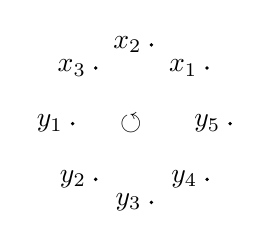
\begin{tikzpicture}
\begin{scope}
\node[left] at (0,0) {$\circlearrowleft$};

\foreach \x in {1,...,3}
{
 \pgfmathsetmacro\myangle{\x*45}
\filldraw[black] (\myangle:1cm) circle (0.4pt) node[left]{$x_{\x}$};
}
\foreach \x in {1,...,5}
{
 \pgfmathsetmacro\myangle{(\x+3)*45}
  % \pgfmathsetmacro\y{\x-3}
\filldraw[black] (\myangle:1cm) circle (0.4pt) node[left]{$y_{\x}$};
}
 \end{scope}
\end{tikzpicture}
\end{center}
\caption{An order in which $X = \{x_1,x_2,x_3\} \in [8]^{(3)}$ is an interval, where we've enumerated $[8]\setminus X = \{y_1,\dotsc,y_5\}$.} \label{fig:X_interval_circ_order}
\end{marginfigure}
In how many circular orders is a given $X\in [n]^{(r)}$ an interval? To obtain an interval, we order the elements of $X$ in $r!$ ways, and then order the rest of the set in $(n-r)!$ ways, yielding $r!(n-r)!$ orders in which $X$ is an interval. See \cref{fig:X_interval_circ_order} for an illustration. 

We have at most $r$ sets of $\F$ as intervals per circular order, and $(n-1)!$ circular orders, so at most $r(n-1)!$ sets in $\F$ over all circular orders.

On the other hand, each set of $\F$ has only $r!(n-r)!$ orders in which it is an interval. Thus, we have $|\F| r!(n-r)!$ intervals corresponding to sets in $\F$, counted over all orders. Hence,
\[
|\F| r! (n-r)! \leq r(n-1)! 
\]
which completes the proof.
\end{proof}

\begin{remark}
For $r < n/2$, if $\F\subset [n]^{(r)}$ is intersecting and has maximal size, i.e. $|\F| = {n-1\choose r-1}$, then for some $x\in n$, we have
\[
\F = \{A\in [n]^{(r)}: x\in A \}.
\]
The proof is left as an exercise. In particular, there are only $n$ possible extremal families.

Consider $r=n/2$. For each set $A \in [n]^{(r)}$, there is only one forbidden set $A^c$. So $\F$ may be formed by choosing one set $A$ from each pair $\{A,A^c\}$ arbitrarily. This yields a doubly-exponential number of extremal families.
\end{remark}

\newthought{We will now consider} a generalization of intersecting.
% \begin{definition}
We say $\F\subset [n]^{(r)}$ is \defn{$t$-intersecting}[t-intersecting] if $|A\cap B|\geq t$ for all $A,B\in \F$.
% \end{definition}
We wish to find $m(n,r,t)$, the maximum size of a $t$-intersecting family $\F$ which is a subset of $[n]^{(r)}$.
A natural guess of an optimal family would be 
\[
 \F_0 := \F_0(n,r,t) = \{ A \in [n]^{(r)}: L\subset A\}
\] for some $L\subset [n]$ with $|L| = t$.
Note $|\F_0| = {n-t \choose r-t}$.
On the other hand, for which $n,r,t$ is $m(n,r,t) = {n\choose r}$? I.e., when is the family $[n]^{(r)}$ itself $t$-intersecting?
We may use the inequality
\[
t\leq |A\cap B| \leq |A| + |B| -  |A\cup B| = 2r - n
\]
to obtain the bound $2r-t \geq n$. So, as with the $1$-intersecting case, for large enough $r$ (compared to $t$ and $n$), $[n]^{(r)}$ itself is intersecting.

What about $n=2r-t+1$? Then $|\F_0| = {2r-2t+1 \choose r-t}$. But we could still take all $r$ element subsets of $[n-1]$ to obtain
\[
m(n,r,t) \geq {2r -t \choose r}.
\]
But
\[
{2r -t \choose r} > {2r-t+1 \choose r} \geq {2r -2t+1 \choose r-t}.
\]
So $\F_0$ does not achieve the maximum in this case either.

\begin{exercise}
Prove that $\F_0$ is optimal when $n$ is large compared to $r$ and~$t$.\marginnote{This is the content of \cref{thm:F0max}.}
\end{exercise}

\lect{1}{26}
% \marginnote{Lecture 6: Monday, January 26, 2016.}


Now, consider the family
\[
\F_{r-t} := \{ A\in [n]^{(r)}: |L\cap A|\geq r\}
\]
for some $L$ with $|L| = 2r-t$.
 % maybe: 
 % When $n \leq 2r-t$, we may choose all of $[n]^{(r)}$, and this family is optimal.
Define an interpolation between $\F_0$ and $\F_{r-t}$ by 
\[
\F_k := \{A\in [n]^{(r)}: |A\cap L|\geq k+t\}
\]
for $|L| = 2k+t$.
Then for $A,B\in \F_k$ we have
\[
|A\cap B\cap L| \geq |A\cap L| + |B\cap L| - |L| \geq 2(k+t) - (2k+t) = t
\]
so for every $0\leq k \leq r-t$, the family $\F_k$ is $t$-intersecting. 
~\begin{margintable}[4cm]
\begin{center}
\begin{tabular}{lccc}\toprule
 & \multicolumn{3}{c}{$k$} \\ \cmidrule(r){2-4} 
 $n$& $0$ &$1$&$2$\\\midrule 
 % & & 0 & 1 & 2\\ \midrule
 $8$ &10 & 16 & \boxed{21}\\
 $11$ & 28 & \boxed{31} & 21\\
 $13$ & \boxed{45}& 41& 21 \\\bottomrule
\end{tabular}
\end{center}
\caption{The size of $\F_k(n)$, given $r=5$ and $t=3$, tabulated over several choices of $k$ and $n$. We see that the maximal $\F_k(n)$ changes based on both $k$ and $n$.}\label{tab:Fks}
\end{margintable}
\begin{example}
Consider $r=5$, $t=3$. Then
\begin{gather*}	
|\F_0(n) | = {n-3 \choose 2}, \\
|\F_1(n)| = {5\choose 4}{n-5 \choose 1} + 1 = 5(n-5)+1,\\
|\F_2(n)| = {7\choose 5} = 21.
\end{gather*}
By choosing different values of $n$ (see \cref{tab:Fks}), we see that the maximum size family occurs at different $k$'s: it is a more complicated situation than the $1$-intersecting case.
\end{example}
In general, for $n\geq 2k+t$,
\[
| \F_k(n)| = \sum_{s=k+t}^{2k+t} {2k+t \choose s} {n-2k-t \choose r-s}
\]
where we are summing over possible sizes $s$ of $|A\cap L|$. The first combination comes from choosing within $L$, and the second from choosing outside of $L$.

We may think of $|\F_k(n)|$ as a function of $n$. Then it is a polynomial of degree $r-k-t$ in which the coefficient of the monomial of largest degree is positive. Among the $\F_k(n)$'s, the family $\F_0(n)$ is eventually of the largest size, because it is the polynomial of highest degree. In fact, $\F_0(n)$ is eventually the largest family overall, as the following result shows.
\begin{theorem} \label{thm:F0max}
For all $r,t$ there exists $n_0$ such that for $n\geq n_0$,
\[
m(n,r,t) = |\F_0| = {n-t \choose r-t}.
\]
\end{theorem}
\begin{proof}	
Let $\F\subset [n]^{(r)}$ be $t$-intersecting such that $|\F| = m(n,r,t)$. Then there exists $A,B\in \F$ such that
\[
|A\cap B| = t
\]
for $n\geq 2r-t$. Assume not. If $\min_{A,B\in \F} |A\cap B| = t+\ell$ for some $\ell\geq 1$, then choose some  $L\subset A\cap B$ with $|L|=\ell$, and consider the set $A'=A\setminus L$. If $A'\in \F$, then we would have $|A'\cap B|=t < t+\ell$, so $A'\not \in \F$. But for any $C\in \F$, we have
\[
t+\ell \leq |A\cap C| = |A'\cap C| + |L\cap C| \leq |A'\cap C| +\ell,
\]
so $|A'\cap C|\geq t$. Thus, $\F\cup \{A'\}$ is $t$-intersecting and $|\F\cup \{A'\}| > |\F|$, which contradicts the maximality of $\F$.

Now, let $Z=A\cap B$, where $|A\cap B|=t$. If $Z\subset C$ for all $C\in \F$, then $|\F| \leq {n-t \choose r-t}$. So we may assume there exists $C\in \F$ such that $Z\not \subset C$. We will show 
\begin{equation}	\label{eq:XcapAcupBcupC_big} \tag{$\star$}
 |X \cap (A\cup B\cup C)|\geq t+1
 \end{equation} for all $X\in \F$. Since each set is of size $r$, the size $L:=|A\cup B\cup C| \leq 3r$. This is enough as it implies
\[
|\F| \leq \sum_{s=t+1}^r {L \choose s} {n-L \choose r-s}
\]
which is a polynomial of degree at most $r-t-1$, and so is eventually less than ${n-t\choose r-t}$, which is a polynomial of degree $n-t$. 

Let us show \eqref{eq:XcapAcupBcupC_big}. We know
\[
X\cap (A\cup B\cup C) = (X\cap A)\cup (X\cap B)\cup (X\cap C).
\]
Each set is of size at least $t$; for $|X\cap (A\cup B\cup C)|\leq t$, then $|X\cap (A\cup B\cup C)| = t$, and in particular,  $Y:=X\cap A= X\cap B = X\cap C$. Then $Y\subset Z$, but since $|Y| = |Z| = t$, we have $Y=Z$. Then we have $Z=Y = X\cap C \subset C$, which is a contradiction.
\end{proof}

The following theorem, presented here without proof, resolves our question.
\begin{theorem}[\cite{Ahlswede-Khachatrian-1997}]
For all $n,r,t$,
\[
m(n,r,t) = \max_k |\F_k|.
\]
\end{theorem}

\newthought{Let us consider} a consequence of \erdos-Ko-Rado\sidenote{\Cref{thm:erdos-ko-rado}}. Let $Z_1,\dotsc,Z_n$ be independent Bernoulli random variables  each  with expectation value $p > \tfrac{1}{2}$. Then $\Pr[Z_i=1] = p$, $\Pr[Z_i = 0] = 1-p$.
Suppose the $Z_i$'s are stocks, and the price of each is $\tfrac{1}{2}$. If we invest \$0.50, then our expected return is \$$p$, no matter how we invest.

Suppose we are very conservative and our goal is to have at least $\tfrac{1}{2}$ in the end. A good strategy is to diversify and invest uniformly in each stock; then the law of large numbers says that as the number of stocks goes to infinity, we almost surely recover our $1/2$.
What's the worst possible strategy? It should be to invest in only 1 stock; in that case, our probability of success is $p$.
\begin{theorem}[\cite{LIGGETT197715}]
Let $Z_1,\dotsc,Z_n$ be independent Bernoulli random variables with expectation value $p$. Let $c_1,\dotsc,c_n\geq 0$ with $\sum c_i =1$. Then
\[
\prob \Big[ \sum_{i=1}^nc_i Z_i \geq \tfrac{1}{2} \Big] \geq p.
\]
\end{theorem}
\begin{proof}	
Assume $c_i >0$ for all $i$, and $n$ odd for simplicity. Let $\F = \{A\subset [n]: \sum_{i\in A} c_i \geq \tfrac{1}{2} \}$. That is, $\F$ is the collection of all sets of r.v. such that if exactly those random variables obtain return 1, we did not lose.
Let $\F_k = \F \cap [n]^{(k)}$ and $f_k = |\F_k|$. Then
\[
\prob \Big[ \sum_{i=1}^n c_i Z_i \geq \tfrac{1}{2}\Big] = \sum_{A\in \F} \prob [ \text{exactly }Z_i \text{ with indicies }i\in A \text{ have value 1}].
\]
If we fix some $A$ of size $k$, what is the probability that these $k$ trials succeed? $p^k(1-p)^{n-k}$. Thus,
\[
\prob \Big[ \sum_{i=1}^n c_i Z_i \geq \tfrac{1}{2}\Big] = \sum_{k=0}^n f_k p^k (1-p)^{n-k}.
\]
Our goal is to show that the LHS is larger than $p$.
\begin{enumerate}[{Fact }1.]
	\item  $\F_k$ is intersecting for each $k < n/2$.

	\begin{subproof}
	Suppose not: then there exists $A,B\in \F_k$ such that $A\cap B = \emptyset$. Then $\sum_{a\in A} c_i \geq \frac{1}{2}$, and $\sum_{a\in B} c_i \geq \frac{1}{2}$. But since each $c_i>0$, we must have $A\cup B = [n]$, but we know $|A\cup B|< 2\cdot n/2=n$.
	\end{subproof}

	\item[Corollary.] For $k<n/2$, we have $f_k \leq {n-1\choose k-1}$ by \erdos-Ko-Rado. \marginnote{This corollary is the essential idea of the proof; the algebraic computation later is long but trivial.}
	\item $f_k + f_{n-k} \geq {n\choose k}$ for all $k$.

	\begin{subproof}
	For every $A$, either $A\in \F$ or $[n]\setminus A \in \F$: if the sum of some collection of $c_i$ is less than one half, then the sum of the rest must be at least one half. Thus, for $A\in [n]^{(k)}$, either $A\in \F_k$, or $[n]\setminus A\in \F_{n-k}$, and $f_k + f_{n-k} \geq |[n]^{(k)}| = {n\choose k}$.
	\end{subproof}
\end{enumerate}
Now, 
\begin{align*}	
\sum_{k=0}^n f_k p^k (1-p)^{n-k}&= \sum_{k<n/2} (f_k + f_{n-k}) p^{n-k}(1-p)^k \\
&\qquad+ \sum_{k< n/2}  f_k ( p^k (1-p)^{n-k}) - p^{n-k}(1-p)^k).\\
\intertext{By fact 2,}
&\geq \sum_{k<n/2}{n\choose k} p^{n-k}(1-p)^k \\
&\qquad+ \sum_{k< n/2}  f_k ( p^k (1-p)^{n-k}) - p^{n-k}(1-p)^k).\\
\intertext{Since $ p^k (1-p)^{n-k}) - p^{n-k}(1-p)^k < 0$,  the corollary to fact 1 yields}
&\geq \sum_{k<n/2} {n\choose k}p^{n-k}(1-p)^k \\
&\qquad+ \sum_{k< n/2}  {n-1\choose k-1}( p^k (1-p)^{n-k}) - p^{n-k}(1-p)^k). \\
\intertext{Now we may group powers of $p$ to obtain}
&= \sum_{k<n/2} p^{n-k} \left[ {n\choose k}(1-p)^k - {n-1 \choose k-1}(1-p)^k  \right] \\
&\qquad\qquad +p^k \left[ {n-1\choose k-1}(1-p)^{n-k} \right].\\
\intertext{We may pull out $(1-p)^k$ of the first term, and use that ${n\choose k}- {n-1 \choose k}={n-1\choose k-1}$ to obtain}
&= \sum_{k<n/2} p^{n-k} \left[ {n-1\choose k-1}   \right](1-p)^k + p^k \left[ {n-1\choose k-1} \right](1-p)^{n-k}.\\
\intertext{Now, in first term we may switch to summing over $k>n/2$, swapping $n-k$ with $k$ to get}
&= \sum_{k>n/2} p^{n-k} \left[ {n-1\choose k-1}   \right](1-p)^k \\
&\qquad+\sum_{k<n/2} p^k \left[ {n-1\choose k-1} \right](1-p)^{n-k}.\\
% &= \sum_{k<n/2} {n-1\choose k-1} p^k(1-p)^{n-k} \\
% &\qquad+ \sum_{k>n/2} \Bigg({n\choose k}- {n-1 \choose k} \Bigg) p^k(1-p)^{n-k}\mathnote{Using ${n-1\choose k-1}={n\choose k}- {n-1 \choose k}$.}\\
&=\sum_{k=1}^n {n-1 \choose k-1} p^k (1-p)^{n-k}\\
&= p \sum_{\ell=0}^{n-1} {n-1 \choose \ell} p^\ell (1-p)^{n-1-\ell} \\
&= p( p + (1-p))^{n-1} =p. \qedhere 
\end{align*}
\end{proof}
\begin{fullwidth}
\printbibliography[segment=\therefsegment,heading=subbibliography]
\end{fullwidth}


\clearpage
\newrefsegment
%!TEX root = ../CombinatoricsNotes.tex

\section{Compression and Shadows} %\marginnote{Lecture 7: Wednesday, January 27, 2016.}
\lect{1}{27}
As an aside, let's consider Steiner symmetrization\sidenote{\cite{steiner1838einfache}}, a technique in geometry.
Given a shape $K\subset \R^2$, with a line of ``symmetry'' $L$, we obtain $S_L(K)$ from $K$ by replacing $K\cap L'$ for every line $L'$ orthogonal to $L$ by an interval of length equal to $|K\cap L'|$ centered at $L$.
\paragraph{Properties:}
\begin{enumerate}
	\item $\area(S_L(K)) = \area(K)$
	\item $\diam(S_L(K)) \leq \diam (K)$ \marginnote{The diameter is the largest distance between two points on $K$. We may prove this by drawing trapezoids between two lines $L'$ and $L''$, one of which passes through each point (close to) achieving the diameter.}
	\item $\perim(S_L(K)) \leq \perim(K)$.
\end{enumerate}
Given a shape in $\R^2$ with area 1, what is the smallest diameter? That's the diameter of the area 1 disc. Sketch of proof: take the shape acheiving minimum diameter. By a compactness argument, we could show that if we ``repeatedly'' symmetrize, eventually it is symmetric across every line.

If some bounded shape is symmetric with respect to reflection about three lines $L_1, L_2,$ and $L_3$, then $L_1,L_2,L_3$ all go through the same point. Why? The center of mass must lie on each line.
This will show us that we have a disk. Let us consider a discrete to this symmetrization process: \defn{compression}.
For $A\in [n]^{(r)}$, set
\[
R_{ij}(A) = \begin{cases}
(\A\setminus \{j\})\cup \{i\}, & \text{if } j\in A, i\not \in A\\
A, & \text{otherwise}.
\end{cases}
\]
For example,
\begin{gather*}	
R_{15}(\{2,3,5\}) = \{1,2,3\}, \qquad
R_{15}(\{2,3,4\}) = \{2,3,4\},\\
R_{15}(\{1,3,5\}) = \{1,3,5\}.
\end{gather*}
Let $\tilde{R}_{ij}(\A) = \{R_{ij}(A): A\in \A\} \cup \{A: R_{ij}(A)\in \A \}$. \marginnote{Intuition: $\tilde{R}_{ij}$ applies $R_{ij}$ unless the resulting set is already in $\A$, to prevent collapse.}

\paragraph{Properties:}
\begin{enumerate}
	\item $|\tilde{R}_{ij}(\A)| = |\A|$.

	Let $P_{ij} \subset [n]^{(r)}$ denote the collection of all sets containing $j$ but not $i$. Then $R_{ij}: P_{ij} \to P_{ji}$  is bijection.
\end{enumerate}


\noindent We will say $\A$ is \defn{compressed} if $\tilde{R}_{ij}(\A)= \A$ for all $i<j$.
\begin{enumerate}\setcounter{enumi}{1}
\item Any set system $\A$ can be made compressed by applying finitely many compression operators $\tilde{R}_{ij}$, for $i<j$.

Let $w(A) = \sum_{i\in A} i$, and $w(\A) = \sum_{A\in \A} w(A)$. Then $w(R_{ij}(A)) \leq w(A)$ with equality iff $R_{ij}(A)=A$. Therefore, $w(\tilde{R}_{ij}(\A))\leq w(\A)$ with equality iff $\tilde{R}_{ij}(\A) = \A$. Therefore, the process must stop, because we start with finite integer weight and the weight may only decrease (and may not be negative).
\end{enumerate}


In human terms, a compressed set system is one where if we try to replace any element of a set with a smaller element, we end up with something already in the set system.
Let us define a natural partial order on $[n]^{(r)}$. If $A = \{a_1,\dotsc,a_r\}$ with $a_1 < a_2 < \dotsb < a_r$, and $B = \{b_1,\dotsc,b_r\}$ with $b_1<\dotsb < b_r$, then we say $A\preceq B$ if $a_i\leq b_i$ for all $i=1,\dotsc,r$.


\begin{enumerate} \setcounter{enumi}{2}
\item If $i<j$, then $R_{ij}(A) \preceq A$, and conversely if $A' \preceq A$, then $A'$ can be obtained from $A$ by using finitely many compression operators $R_{ij}$ for $i<j$.

\end{enumerate}
Therefore, $\A$ is compressed if and only if for every $A\prec B$ with $B\in \A$, we have that $A\in \A$. In otherwords, $\A$ is an ideal in this order. See \cref{fig:compressed_sets_partial_order} for an example.
\begin{marginfigure}
\begin{center}
\begin{tikzcd}
& \boxed{\{1,2\}} \arrow{d}\\
&\boxed{\{1,3\}} \arrow{ld} \arrow{rd}\\
\boxed{\{1,4\}} \arrow{d} \arrow{rrd}  & &\boxed{\{2,3\}} \arrow{d}\\
\boxed{\{1,5\}} \arrow{d}&& \boxed{\{2,4\}}\arrow{d} \arrow{lld}\\
\{2,5\} \arrow{rd} && \boxed{\{3,4\}} \arrow{ld}\\
&\{3,5\} \arrow{d}\\
&\{4,5\}
\end{tikzcd}
\end{center}
\caption{The partial order on $[5]^{(2)}$, where $A\rightarrow B$ means $a \prec b$, and different sets in the same row are incomparable. The boxed elements together form a compressed set.} \label{fig:compressed_sets_partial_order}
\end{marginfigure}

\begin{enumerate}\setcounter{enumi}{3}
	\item  If $\A$ is intersecting, then $\tilde{R}_{ij}(\A)$ is intersecting.
	Suppose not. Then there exists $A,B\in \tilde{R}_{ij}(\A)$ such that $A\cap B= \emptyset$. If both $A,B\in \A$, then they are intersecting, so let $A\not \in \A$. Then $A = R_{ij}(A')$ for some $ A'\in \A$ with $j\in A'$. Now, if $B \not \in \A$ too, then $B = R_{ij}(B')$ for some $B'\in \A$ with $j\in B'$, and we'd have $i\in A\cap B$, which is a contradiction. So $B\in \A$ with $i\not\in B$.  If $B= R_{ij}(B)$, then $R_{ij}(B)\in \A$. Otherwise, we have $j \in B$, and we must  have $B \neq R_{ij}(B')$ for every $B'\in \A$ (for   $B\in P_{ij}$, while the image of $R_{ij}$ is  $P_{ji}$ which is disjoint from $P_{ij}$). In this case then, since $B\in \tilde{R}_{ij}(\A)$, we must then have $R_{ij}(B)\in \A$ too. So in either case, $R_{ij}(B)\cap A'\in \A$ which is intersecting, so $R_{ij}(B)\cap A' \neq \emptyset$.

	% Now, $k\neq j$ has $k\in A'\cap B$, then  then $k \in R_{ij}(A') = A$, so $k\in A\cap B$, which is a contradiction. On the other hand, $A'\cap B\neq \emptyset$ since $A',B\in \A$ which is intersecting. So $A'\cap B = \{j\}$, and thus $j\in B$. So $B\in P_{ij}$. So $R_{ij}(B) \neq B$, and $B\in \tilde{R}_{ij}(\A)$, so $B$ is such that $R_{ij}(B) \in \A$ (otherwise $B$ would be the non-trivial image of some $B'$ under $R_{ij}$, which leads to a contradiction as showed earlier). Thus $R_{ij}(B)\cap A' \neq \emptyset$.



	%   So $A',B\in \A$, and thus $A'\cap B\neq \emptyset$.



	% Suppose not. Then there exists $A,B\in \tilde{R}_{ij}(\A)$ such that $A\cap B = \emptyset$. We may assume that $\A \not \ni A = R_{ij}(A')$ for some $A'\in \A$, and $B\in \A$\sidenote{Otherwise $i\in B$, so $A\cap B \ni i$.}, and $A'\cap B = \{j\}$. So $B\in P_{ij}$, and hence was unchanged by $R_{ij}$, 


	% so $R_{ij}(B)\in \A$. Then $A'\cap R_{ij}(B) \neq \emptyset$, since $\A$ is intersecting.

	But $A'$ is obtained from $A$ by changing $j$ to $i$, and $R_{ij}(B)$ is obtained from $B$ by changing $j$ to $i$, so if $A'\cap R_{ij}(B) \neq \emptyset$, then we have $A\cap B\neq \emptyset$.



\end{enumerate}

\begin{proof}[Proof of \erdos-Ko-Rado theorem by compression]
We wish to show that if $r\leq n/2$, $\A\subset [n]^{(r)}$ is intersecting, then
\[
|\A| \leq {n-1 \choose r-1}.
\]
We will proceed by induction on $n$ and $r$. The case $r=n/2$ is easy: ${n-1\choose r-1} = \frac{1}{2}{n\choose r}$, and sets in $[n]^{(r)}]$ are just complementary pairs.

Assume $r<n/2$. By the facts we have proven, we may assume $\A$ is compressed. Let
\begin{align*}
\A_0 &= \{A\in \A: n\not\in \A\}, & \A_1 &= \{A\in \A: n\in A\}.
\end{align*}
Then by the IH,
\[
|\A| = |\A_0| + |\A_1| \leq {n-2 \choose r-1} + |\A_1|
\]
If $|\A_1| \leq {n-2 \choose r-2}$, then\sidenote{using ${n-2 \choose r-1} + {n-2 \choose r-2} = {n-1\choose r-1}$} we have $|\A| \leq {n-1\choose r-1}$.
Let 
\[
\A_1 \setminus \{n\} := \{A-\{n\}: A\in \A_1\}.
\]
 If $\A_1\setminus \{n\}$ is intersecting, then $|\A_1\setminus \{n\}| \leq {n-2 \choose r-2}$ by the IH, since $\A_1\setminus \{n\} \subset [n-1]^{(r-1)}$. 
Suppose $\A_1\setminus \{n\}$ is not intersecting. Then there exists $A,B\in \A$ such that 
\[
A\cap B = \{n\}.
\]
Because $2r<n$, there exists $i<n$ such that $i\not \in A\cup B$. Then $R_{in}(B) \in \A$ since $\A$ is compressed.
But $A\cap R_{in}(B) = \emptyset$, contradicting that $\A$ is intersecting. 
\end{proof}

Let $\A\subset [n]^{(r)}$, with $|\A| = m$. What is $\min |\partial \A|$? \marginnote{Recall: 
\[
\partial A = \{B \in [n]^{(r-1)}: B\subset A \text{ for some } A\in \A\}.
\]}
We know the local LYM inequality:
\begin{equation*}	\tag{\cref{eq:local_LYM}}
\frac{|\partial A|}{{n\choose r-1}}\geq \frac{|\A|}{{n\choose r}}
\end{equation*}
but this is rarely tight.

Let's consider $m=1$, that is, $|\A|=1$. Then the answer is $r= {r\choose r-1}$. For $m=2$, the answer is $2r-1$, because their shadows can at most share 1 set.
For $r=2$, we have a simple graph with $m$ edges. What is the minimal number of verticies? We want the minimal $n$ so that $m\leq {n \choose 2}$.
\lect{2}{1}
% \marginnote{Lecture 8: Monday, February 1, 2016.}
Let us change our question to consider $\A\subset \N^{(r)}$ . Given $r$ and $m$, what is $\min |\partial \A|$ given $\A\subset \N^{(r)}$ with $|\A| = m$?

\begin{lemma} \label{lem:compression_decreases_size_of_shadow}We have that
\[
|\partial \tilde{R}_{ij}(\A)| \leq |\partial \A|
\]
for every $\A\subset \N^{(r)}$.
\end{lemma}
\begin{proof}	

It suffices to show that
\marginnote{ $|X|\geq |Y| \iff |X\setminus Y| \geq |Y\setminus X| $ because $|X| = |X\setminus Y| + |X \cap Y|$ and $|Y| = |Y\setminus X| + |X\cap Y|$. }
\[
|\partial \tilde{R}_{ij}(\A)\setminus(\partial \A)| \leq | \partial A\setminus(\partial \tilde{R}_{ij}(\A))|.
\]
If $B\in \partial \tilde{R}_{ij}(\A)\setminus (\partial \A)$, then $i\in B$ but $j\not\in B$. Let's see why this is true. Let $A\in  \tilde{R}_{ij}(\A)\setminus (\A)$ such that $B = A\setminus\{k\}$ for some $k$. Then $i\in A$, $j\not \in A$ (and so $j\not \in B$ too). Now, if $i\not \in B$, then $k=i$. But then $B = R_{ji}(A)\setminus\{j\}$ so $B\in \partial \A$, a contradiction.



It is enough to show that
\[
R_{ji}(B)\in \partial \A\setminus(\partial \tilde{R}_{ij}(\A)).
\]
Clearly, $R_{ji}(B)\in \partial \A$, since $B= A\setminus\{k\}$ with $k\neq i,j$, so $R_{ji}(B) = R_{ji}(A)\setminus\{k\}$.

The last piece to check is that $R_{ji}(B)\not\in \partial \tilde{R}_{ij}(\A)$. If that were the case, then $R_{ji}(A)\setminus\{k\} \subset C$ for some $C \in \tilde{R}_{ij}(\A)$. Since $j\in R_{ji}(A)$ and $k\neq j$, we have $j\in C$. Then $R_{ij}(C) \in \A$. But then $B=A\setminus \{k\} \in R_{ij}(C) \in \A$, so $B \in \partial \A$, a contradiction.
% Assume $B= C \setminus \{\ell\} \in \partial \tilde{R}_{ij}(\A)$ for some $C \in \tilde{R}_{ij}(\A)$. Then $C\setminus\{\ell\} = R_{ji}(A)\setminus \{k\}$.
% \understand
\end{proof}
This lemma shows that for the purposes of minimizing $|\partial \A|$, we may start with a compressed set.

\newthought{We defined a partial order} on $\N^{(r)}$ by $A = \{a_1,\dotsc,a_r\}$, $a_1<a_2<\dotsb < a_r$, and $B=\{b_1,\dotsc,b_r\}$, and $b_1<b_2<\dotsb < b_r$, then $A\preceq B$ if $a_i\leq b_i$ for $i\in[r]$.
We may define the \defn{lexicographic order} on $\N^{(r)}$. We say $A\leq_L B$ if ($a_1<b_1$) or ($a_1=b_1$ and $a_2 < b_2$) or $(a_1 = b_1$ and $a_2=b_2$, but $a_3<b_3)$ etc. That is, either $A=B$, or if $s$ is the minimal index such that $a_s\neq b_s$, then $a_s<b_s$. See \cref{fig:53_lexographic_order} for an example.
\begin{marginfigure}
\begin{tikzcd}[column sep=small]
\boxed{\{1,2,3\}} \arrow{r} & 
\boxed{\{1,2,4\}} \rar \snakesetup &
\{1,2,5\} \snakearrow{lld}  \\
\boxed{\{1,3,4\}} \rar &
\{1,3,5\} \rar \snakesetup&
\{1,4,5\}  \snakearrow{lld}\\
\boxed{\{2,3,4\}} \rar \snakesetup &
\{2,3,5\}  \rar   &
\{2,4,5\}   \snakearrow{lld}\\
\{3,4,5\}
\end{tikzcd}

\caption{Elements of $[5]^{(3)}$ in lexographic order, where $A\imp B$ means $A\leq_L B$. The subsets of $[4]^{(3)}$ are boxed; they appear in order, but not next to each other.} \label{fig:53_lexographic_order}
\end{marginfigure}

Consider the lexographic order on $\N^{(3)}$. What is the 100th smallest set in this order? $\{1,2,102\}$.


Now, let us define the \defn{colexicographic order} on $\N^{(r)}$. Define $A\leq B$ if $a_r<b_r$ or ($a_r=b_r$ and $a_{r-1} <b_{r-1}$) or \ldots etc. We may write this as $A=B$ or if $s$ is the maximal index such that $a_s\neq b_s$, then $a_s<b_s$. 



% \begin{fullwidth}

\begin{figure*}[ht]
% \makeatletter\setlength\hsize{\@tufte@fullwidth}\setlength\linewidth{\@tufte@fullwidth}\let\caption\@tufte@orig@caption\makeatother
\centering

\begin{tikzcd}[column sep=small]
[3]^{(3)} &\{1,2,3\} \arrow{d} \\
 {[4]^{(3)}}\setminus[3]^{(3)} & \{1,2,4\} \arrow{r}& \{1,3,4\} \snakesetup \arrow{r}& \{2,3,4\} \snakearrow{lld}\\
{[5]^{(3)}}\setminus[4]^{(3)} & \{1,2,5\} \arrow{r} & \{1,3,5\}\arrow{r} & \{2,3,5\} \arrow{r}& \{1,4,5\} \arrow{r}& \{2,4,5\}\arrow{r} & \{3,4,5\}
\end{tikzcd}
\bigskip
\caption{Elements of $[5]^{(3)}$ in colexographic order. Note that $[n]^{(r)}$ is an initial segment of the colex order on $\N^{(r)}$. \label{fig:53_colexographic_order}} 
\end{figure*}
% \end{fullwidth}

\begin{theorem}[\cite{kruskal1963,katona1968}] \label{thm:kruskal_katona}
If $\A\subset \N^{(r)}$ with $|\A| = m$, then $|\partial \A|$ is at least as large as the size of the shadow of the first $m$ elements of $\N^{(r)}$ in colexicographic order.
\end{theorem}
\begin{example}
If $A= \{10,7,3\}$ what is the position of $A$ in the colex order on $\N^{(3)}$? In the rows\sidenote{Referring to an analogous diagram to \cref{fig:53_colexographic_order}.} before $A$, there will be $|[9]^{(3)}| ={9\choose 3}$ elements.  In the row containing $A$, there are sets of the form $\{10,x,*\}$ with $x<7$, i.e. ${6\choose 2}$ sets. Next, there are sets of the form $\{10,7,y\}$ with $y<3$, i.e. ${2\choose 1}$ sets. Finally, we have our set, $\{10,7,3\}$. In total then,
\[
{9\choose 3} + {6\choose 2} + {2\choose 1} + 1 = 102.
\]

See \cref{fig:colex_near_A} for a diagram.
\begin{figure*}[ht]
\begin{center}
\begin{tikzcd}[column sep=tiny]
  \{10,6,5\} \rar&\{10,7,1\} \rar &\{10,7,2\} \rar &\{10,7,3\} \rar  & \{10,7,4\}  \rar & \{10,7,5\}\rar   & \{10,7,6\}  \rar & \{10,8,1\}.
\end{tikzcd}
\caption{The colex order near $A=\{10,7,3\} \subset \N^{(3)}$. The notation $A\imp B$ means $A\leq B$ in colex order. Since $A$ is the 102nd set in colex order on $\N^{(3)}$, $\{10,7,1\}$ is the 100th set which provides a nice comparison to $\{1,2,102\}$, the 100th set in lexicographic order. In particular, we note that in colex order, every set is finitely many positions away from the smallest set, while in lexicographic order many sets are infinitely far (like $\{1,3,4\}$).}\label{fig:colex_near_A}
\end{center}

\end{figure*}
% \improvement{Put captions of full-width figures below the figure in the main column.}
\end{example}


% \begin{definition}
For $A\in \N^{(r)}$, let the \defn{initial segment of $A$} be $I(A) =\{B: B\leq \A\}$ and let $i(A) = |I(A)|$. 
% \end{definition}
\begin{lemma}
If $A = \{a_1,\dotsc,a_r\}$ with $a_r>a_{r-1}>\dotsb> a_1$ then 
\[
i(A) = {a_{r}-1\choose r} + {a_{r-1}-1 \choose r-1} + \dotsb + {a_1-1 \choose 1} + 1.
\]
\end{lemma}
\begin{proof}	
${a_{k} -1\choose k}$ counts sets $B\subset A$ which coincide with $A$ over 
\[
 a_r,a_{r-1},\dotsc,a_{k+1}
\]
  but whose $k$th largest element is smaller.
\end{proof}

\begin{lemma} We have that the shadow of the inital segment $I(A)$ is the initial segment of $A\setminus\{\min A\}$. That is,
\[
\partial I(A) = I( A\setminus \{\min A\}).
\]
\end{lemma}
\begin{proof}	
If $A = \{a_r,\dotsc,a_2,a_1\}$, then we wish to show that $B\subset \N^{(r-1)}$ is in $\partial I(A)$ if and only if $B \leq \{a_r,\dotsc,a_2\} = A\setminus \{\min A\}$ in colex order. This is left as an exercise. One way to proceed is by induction on $r$, splitting into cases where $B$ contains $a_r$ or not.
% \add{proof.}
\end{proof}

\begin{corollary}
If  
\[
 i(A) = {a_r-1\choose r} + {a_{r-1} \choose r-1} + \dotsb + {a_1-1\choose 1} + 1,
 \]
then 
\[
|\partial (I(A))| = {a_r -1\choose r-1} + {a_{r-1} -1 \choose r-2} + \dotsb + {a_2-1 \choose 1} + 1.
\]
\end{corollary}

Let us restate \cref{thm:kruskal_katona}:
\begin{theorem*}[Kruskal--Katona]
Let $\A\subset \N^{(r)}$ with 
\[
|\A| = {a_r-1\choose r} + {a_{r-1} -1\choose r-1} + \dotsb + {a_1-1\choose 1} + 1
\]
for some $a_r>\dotsc>a_1$. Then
\[
|\partial \A| \geq{a_r -1\choose r-1} + {a_{r-1} -1 \choose r-2} + \dotsb + {a_2-1 \choose 1} + 1.
\]
\end{theorem*}
\begin{remark}
For every positive integer $m$, we may write $m$ as 
\[
m={a_r-1\choose r} + {a_{r-1} \choose r-1} + \dotsb + {a_1-1\choose 1} + 1
\]
for some $a_r> a_{r-1} > \dotsm > a_1$. We have shown this already by considering the $m$th element in colex order of $\N^{(r)}$.
\end{remark}

\begin{proof}[Proof by induction on $r$; for fixed $r$, by induction on $|\A|$.] The base case $r=1$ is trivial. For the induction step, we will assume that $\A$ is compressed, by \cref{lem:compression_decreases_size_of_shadow}. Let
\begin{align*}	
A_1 :\!&= \{A\in \A: 1\in A\}, & A_0 :\!&= \A\setminus \A_1.
\end{align*}

\begin{enumerate}[{Claim} 1:]
\item $|\A_1| \geq |\partial A_0|$.\marginnote{Compression pushes us towards smaller elements, so $\A_1$ should be large.}

\begin{subproof}	
The map $A\mapsto A\cup\{1\}$ is an injection from $\partial \A_0$ to $\A_1$, by compression.
\end{subproof}
	\item
	\[
	|\A_1|\geq {a_r-2\choose r-1} + {a_{r-1}-2\choose r-2} + \dotsb + {a_2-2\choose 1} + 1.
	\]
	\begin{subproof}Assume not. Since $|\A_0| =|\A| - |\A_1|$, we have then have
	\begin{align*}	
	|\A_0|&> \left( {a_r-1\choose r} - {a_r-2\choose r-1} \right) + \left( {a_{r-1}-1\choose r-1} - {a_{r-1}-2\choose r-2} \right) + \dotsb + {a_1-1 \choose 1}\\
	&= {a_{r}-2 \choose r} + {a_{r-1}-2\choose r-1} + \dotsb + {a_1-2 \choose 1}+1.
	\end{align*}
	By the IH\sidenote{Since $\A$ is compressed it must contain 1}, 
\[
|\partial \A_0| \geq {a_r-2\choose r-1} + \dotsb + {a_2-2\choose 1}+1
\]
Then claim 1 yields the result.
	\end{subproof}
\end{enumerate}
Let $B = \{A-\{1\}: A\in \A_1\}\subset \N^{(r-1)}$. Note $|B| = |\A_1|$.
\begin{enumerate}[{Claim} 1:]
\setcounter{enumi}{2}
	\item 
	$|\partial \A|\geq |B| + |\partial B|$.

	\begin{subproof}	
	Note $B\subset \partial \A$. Let $B' = \{B\cup \{1\}: B\in \partial B\} \subset \partial A$. Then $B\cup B' \subset \partial \A$. But since sets in $B'$ contain $1$ and sets in $B$ do not contain $1$, $|B\cup B'| = |B|+|B'|$.
	\end{subproof}
\end{enumerate}
By claims 2, 3, and the IH, we have
\begin{align*}	
|\partial \A| &\geq |B| + |\partial B| \\
&\geq {a_r-2 \choose r-1} + {a_{r-1}-2\choose r-2} + \dotsb + {a_2-2\choose 1}+1 \\
&\qquad + {a_r-2 \choose r-2} + {a_{r-1}-2 \choose r-3} + \dotsb + {a_3-2\choose 1} + 1\\
&= {a_r-1\choose r-1} + \dotsb {a_3-1\choose 2} + {a_2-1\choose 1}+1.  \qedhere
\end{align*}
\end{proof}
\begin{theorem}[\cite{lovaszbook_hyper}]
Let $\A\subset \N^{(r)}$, where $|\A| = {x\choose r}$ for $x\in \R$.\marginnote{We define ${x\choose r} := \frac{x(x-1)\dotsm(x-r+1)}{r!}$. Since the polynomials
${x\choose r}$ and ${x-1\choose r} + {x-1\choose r-1}$ agree on the integers, they agree everywhere.}
Then $|\partial \A| \geq {x\choose r-1}$.\sidenote{If $x$ is an integer, then equality can be achieved by taking $\A=[x]^{(r)}$.}.
\end{theorem}
\begin{proof}	
The proof follows that of the reformulated Kruskal--Katona. Claims 1 \& 3 have the same proof. For claim 2, there is a much simpler proof:
\begin{enumerate}[{Claim }1.]\setcounter{enumi}{1}
% \item $|\partial \A_0|\leq|\A_1|$
\item $|\A_1|\geq {x-1\choose r-1}$.
\begin{subproof}	
If not, $|\A_0| = |\A| - |\A_1| \geq {x\choose r} - {x-1 \choose r-1} = {x-1\choose r}$. Then $|\partial \A_0| \geq {x-1\choose r-1} > |\A_1|$, a contradiction.
\end{subproof}
% \item 
\end{enumerate}
The rest of the proof is the same.
\end{proof}


\begin{corollary} \label{cor:ell_shadows}
Let $\A\subset \N^{(r)}$ with $|\A| = {x\choose r}$ for $x\in \R$. Let 
\[
\partial^{(\ell)}\A = \{B\in \N^{(r-\ell)}: B\subset A \text{ for some }A\in\A\}.
\]
Then
\[
|\partial^{(\ell)}A|\geq {x\choose r-\ell}.
\]
\end{corollary}
\begin{proof}[Proof by induction on $\ell$.] The base case is Lor\'asz's theorem. Then
\[
\partial^{(\ell)}\A = \partial ( \partial^{(\ell-1)}\A)
\]
so the IH and Lor\'asz's theorem yield the result.
\end{proof}

\begin{corollary}
Let $G$ be a 2-graph. Then \marginnote{$\edges (G)$ denotes the edge set of $G$. We identify $G$ with $\edges (G)$.}
\[
|G| = |\edges (G)| = {x\choose 2}
\]
for some $x\in \R$. Then $G$ contains at most ${x\choose k}$ complete subgraphs\sidenote{$k$-tuples of verticies pairwise joined by edges.} of size $k$.
\end{corollary}
\begin{remark}
We may reformulate this as follows, in a special case. Let $G$ be a graph with ${n\choose 2}$ edges (but possibly more than $n$ verticies). Then $G$ contains a maximum number of triangles when $G$ is a complete graph of $n$ verticies. We think of this as we are given a budget of edges, and are trying to maximize the number of triangles we make. Here it is intuitive that to do this, we make a complete graph.
\end{remark}
\begin{proof}	
We may assume that $x\geq k$; otherwise we may not form any complete $k$-subgraphs. If the number of complete subgraphs of $G$ is strictly larger than ${x\choose k}$, then it is equal to ${x' \choose k}$ for some $x' > x$. So we choose $\A$ to be the family of verticies of complete subgraphs of $G$: 
\[
\A = \{V(H): H \text{ is a complete subgraph of }G\} \subset V(G)^{(k)}.
\] Then each $\{x,y\} \in \partial^{(k-2)} \A$ is a two element subset of a complete subgraph of $G$,  so $\partial^{(k-2)} \A\subset \edges(G)$. Then by \cref{cor:ell_shadows}, we must have $|\edges (G)| \geq {x'\choose 2} > {x\choose 2}$, a contradiction.
% \understand
% Everything that lies in the shadow of order $k-2$ must
\end{proof}
\begin{fullwidth}
\printbibliography[segment=\therefsegment,heading=subbibliography]
\end{fullwidth}



\clearpage
\newrefsegment
%!TEX root = ../CombinatoricsNotes.tex

\section{Tur\'an type problems} % (fold)
\label{sec:turian_type_problems}

The general problem we've been considering is to find $\max |\F|$ given that $\F\subset \P([n])$ has certain properties. For example, Sperner systems, and intersecting $r$-graphs. In these problems, we are forbidding certain sub set systems\sidenote{In a Sperner system, there is no 2 element sub system $\{A,B\}$ with $A\subset B$. In an intersecting $r$-graph, there is no two element sub system $\{A,B\}$ with $A\cap B= \emptyset$.}. Here, we will focus on $r$-graphs.  

We will say $\F$ and $\H$ are \defn{isomorphic} set systems if there exists a bijective map $\phi: \bigcup_{F\in \F} F \to \bigcup_{H\in \H}H$ such that $F\in \F$ if and only if $\phi(F)\in \H$.
Now, let forbidden subconfigurations $F_1,\dotsc,F_k$ be given $r$-graphs\sidenote{Recall: Set systems with elements which are in $[n]^{(r)}$.}. Define the \defn{Tur\'an number}
\[
\ex (n; F_1,\dotsc,F_k)
\]
to be the maximum $|\F|$ such that $\F$ does not contain a subgraph isomorphic to any of $F_1,F_2,\dotsc,F_k$.


\begin{remark}
We will increasingly refer to $F\in \F$ as edges.
\end{remark}

\begin{example}
If $M_2$ consists of two disjoint edges of size $r$, then \erdos-Ko-Rado says that $\ex(n;M_2) = {n-1\choose r-1}$ for $n\geq 2r$.\marginnote{Not having a subgraph isomorphic to $M_2$ means there must not be two disjoint subsets in $\F$, i.e., $\F$ is intersecting.}
\end{example}
Let
\[
\pi(n;F_1,\dotsc,F_k) := \frac{\ex(n;F_1,\dotsc,F_k)}{{n\choose r}}
\]
be the ratio of the largest valid size of $\F$ to the size of $[n]^{(r)}$.
We define the \defn{Tur\'an density} of $F_1,\dotsc,F_k$ to be
\[
\pi(F_1,\dotsc,F_k) := \lim_{n\to\infty} \pi(n; F_1,\dotsc,F_k) \in [0,1].
\]

\begin{example}
\[
\pi(M_2) = \lim_{n\to\infty} \frac{{n-1\choose r-1}}{{n\choose r}}=0,
\]
using \erdos-Ko-Rado. \marginnote{If you select two $r$-tuples of elments in an $n$ element set for very large $n$, you almost surely get disjoint tuples.}
\end{example}
\begin{theorem}[\cite{Katona_Nemetz_Simonovits}]
If $r\leq n_0\leq n$, then
\[
\pi(n_0; F_1,\dotsc,F_k) \geq \pi(n; F_1,\dotsc,F_k).
\]\label{thm:pi_decreasing}
\end{theorem}
\begin{remark}
Then $\pi(n;F_1,\dotsc,F_k)$ decreases for $n\geq r$ and is bounded below by zero,  so $\pi(F_1,\dotsc,F_k)$ exists.
\end{remark}
\begin{proof}	
Let $\F\subset[n]^{(r)}$ be such that $|\F| = \ex(n; F_1,\dotsc,F_k)$ and $\F$ contains no subgraphs isomorphic to any of $F_1,\dotsc, F_k$. Let $H_1,H_2,\dotsc,H_N$ be the restrictions\sidenote{Note that for $X\subset [n]$, we define the restriction of $\F$ as $\F\restriction X := \{A\in \F: A\subset X\}$.} of $\F$ to all possible $n_0$ element subsets of $[n]$, where $N = {n\choose n_0}$.
 It suffices to show that
% \begin{align}	\label{eq:pi_avg}
\[
\pi(n; F_1,\dotsc,F_k) = \frac{|\F|}{{n\choose r}} \leq \frac{1}{{n\choose n_0}} \sum_{i=1}^N \frac{|H_i|}{{n_0\choose r}}
\]
% \end{align}
since $\frac{|H_i|}{{n_0\choose r}} \leq \pi(n_0; F_1,\dotsc,F_k)$. \marginnote{This estimate is the only actual inequality in the proof.}

We are left to estimate $\sum_{i=1}^N|H_i|$.
Given an edge in $F\in\F$, how many $H_i$'s does it appear in? Each $H_i$ whose base set\sidenote{Meaning the $n_0$-element set $X$ such that $H_i = \F\restriction X$.} includes $F$, so we need to choose $n_0-r$ more elements for the base set from the $n-r$ remaining possible elements, i.e.  ${n-r \choose n_0-r}$.
Then,
\[
\frac{1}{{n\choose n_0}}\sum_{i=1}^N \frac{|H_i|}{{n_0\choose r}} = |\F| \frac{{n-r\choose n_0 -r}}{{n\choose n_0}{n_0\choose r}}\quad \boxed{=}\quad \frac{|\F|}{{n\choose r}}.
\]
To show the boxed equality and finish the proof, we need
\begin{equation}	\label{eq:binomial_identity_boxes}
{n\choose r}{n-r \choose n_0 -r} = {n\choose n_0}{n_0 \choose r}.
\end{equation}

\lect{2}{3}
% \marginnote[0\baselineskip]{Lecture 9: Wednesday, February 3, 2016}
This is an identity which we can combinatorially reason as follows. The RHS means we first choose $n_0$ elements out of $n$, then choose $r$ out of those $n_0$. The LHS means we choose $r$ elements from $n$ then $n_0-r$ elements from the remaining $n-r$. This is depicted in \cref{fig:binomial_identity_boxes}.

\begin{marginfigure}[0\baselineskip]
\begin{center}
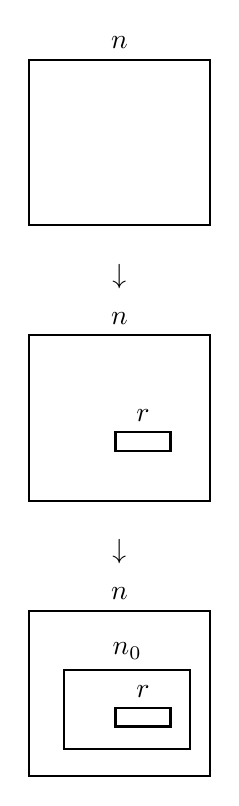
\begin{tikzpicture}

\begin{scope}
\node (rect) at (0,0)[draw,thick,minimum width=2.3cm, minimum height = 2.1cm, label=above:$n$]{};
% \node  at(.1,-.2)[draw,thick,minimum width=1.6cm, minimum height = 1cm, label=above:$n_0$]{};
% \node  at(.3,-.3)[draw,thick,minimum width=.7cm, minimum height = .2cm, label=above:$r$]{};
\end{scope}

\node[yshift=-1.7cm] at (0,0) {$\downarrow$};

\begin{scope}[yshift=-3.5cm]
\node (rect) at (0,0)[draw,thick,minimum width=2.3cm, minimum height = 2.1cm, label=above:$n$]{};
% \node  at(.1,-.2)[draw,thick,minimum width=1.6cm, minimum height = 1cm, label=above:$n_0$]{};
\node  at(.3,-.3)[draw,thick,minimum width=.7cm, minimum height = .2cm, label=above:$r$]{};
\end{scope}
\node[yshift=-5.2cm] at (0,0) {$\downarrow$};

\begin{scope}[yshift=-7cm]
\node (rect) at (0,0)[draw,thick,minimum width=2.3cm, minimum height = 2.1cm, label=above:$n$]{};
\node  at(.1,-.2)[draw,thick,minimum width=1.6cm, minimum height = 1cm, label=above:$n_0$]{};
\node  at(.3,-.3)[draw,thick,minimum width=.7cm, minimum height = .2cm, label=above:$r$]{};
\end{scope}
\end{tikzpicture}\hfill
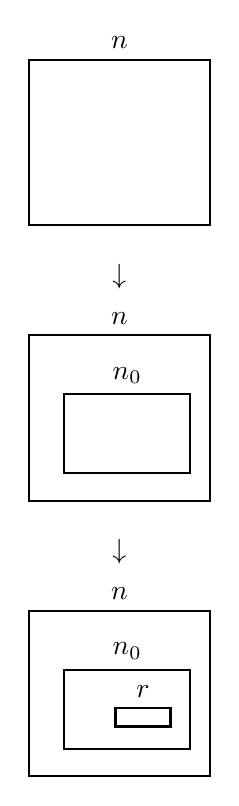
\begin{tikzpicture}
\begin{scope}
\node (rect) at (0,0)[draw,thick,minimum width=2.3cm, minimum height = 2.1cm, label=above:$n$]{};
% \node  at(.1,-.2)[draw,thick,minimum width=1.6cm, minimum height = 1cm, label=above:$n_0$]{};
% \node  at(.3,-.3)[draw,thick,minimum width=.7cm, minimum height = .2cm, label=above:$r$]{};
\end{scope}

\node[yshift=-1.7cm] at (0,0) {$\downarrow$};

\begin{scope}[yshift=-3.5cm]
\node (rect) at (0,0)[draw,thick,minimum width=2.3cm, minimum height = 2.1cm, label=above:$n$]{};
\node  at(.1,-.2)[draw,thick,minimum width=1.6cm, minimum height = 1cm, label=above:$n_0$]{};
% \node  at(.3,-.3)[draw,thick,minimum width=.7cm, minimum height = .2cm, label=above:$r$]{};
\end{scope}
\node[yshift=-5.2cm] at (0,0) {$\downarrow$};

\begin{scope}[yshift=-7cm]
\node (rect) at (0,0)[draw,thick,minimum width=2.3cm, minimum height = 2.1cm, label=above:$n$]{};
\node  at(.1,-.2)[draw,thick,minimum width=1.6cm, minimum height = 1cm, label=above:$n_0$]{};
\node  at(.3,-.3)[draw,thick,minimum width=.7cm, minimum height = .2cm, label=above:$r$]{};
\end{scope}
\end{tikzpicture}
\end{center}
\caption{(above) \emph{Left:} an illustration of the LHS of \cref{eq:binomial_identity_boxes} and \emph{right:} the RHS of \cref{eq:binomial_identity_boxes}. } \label{fig:binomial_identity_boxes}
\end{marginfigure}
\end{proof}

Let $H$ be a graph ($2$-graph). Then $\ex(n,H)=\max |\edges (G)|$, where the maximum is taken over graphs $G$ with $|V(G)| = n$ such that $H$ is not a subgraph of $G$.

We may consider
\[	
\pi(n;H) := \frac{\ex(n,H)}{{n\choose 2}}, \qquad \pi(H):= \lim_{n\to \infty}\pi(n,H).
\]
By \cref{thm:pi_decreasing}, $\pi(n,H)$ decreases for $n\geq 2$ (and fixed $H$), so $\pi(H)$ exists. Let $K_n$ be the complete graph on $n$ verticies: $K_n = [n]^{(2)}$. Since $K_2$ is just a single edge, $\ex(n; K_2)=0$.

Consider
$P_3 =$\scalebox{1}{\begin{tikzpicture}[color=DarkBlue]
\def\n{3}
\def\radius{.6}
\def\rotation{-30}

\def\deg{360/\n}
\pgfmathsetmacro\nminusone{\n-1}

\foreach \x in {1,...,\n}
{
	\pgfmathsetmacro\myangle{\x*\deg+\rotation};
	\filldraw (\myangle:\radius cm) circle (0.4pt) node(a\x){};
}


\foreach \y in {1,...,\n}
{

	\foreach \z in {1,...,\y}
	{
		\ifthenelse{\z < \nminusone}
		{
		\pgfmathsetmacro\myangley{\y*\deg+\rotation}
		\pgfmathsetmacro\myanglez{\z*\deg+\rotation}
		\draw (\myangley:\radius cm) -- (\myanglez:\radius cm);
		}{}

	}
}
\end{tikzpicture}}. Then $\ex(n,P_3) = \floor{n/2}$, and $\pi(P_3)=0$.

Consider $K_3 =$\scalebox{1}{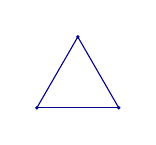
\begin{tikzpicture}[color=DarkBlue]
\def\n{3}
\def\radius{.6}
\def\rotation{-30}

\def\deg{360/\n}
\pgfmathsetmacro\nminusone{\n-1}

\foreach \x in {1,...,\n}
{
	\pgfmathsetmacro\myangle{\x*\deg+\rotation};
	\filldraw (\myangle:\radius cm) circle (0.4pt) node(a\x){};
}


\foreach \y in {1,...,\n}
{

	\foreach \z in {1,...,\y}
	{
		\ifthenelse{\z < \n}
		{
		\pgfmathsetmacro\myangley{\y*\deg+\rotation}
		\pgfmathsetmacro\myanglez{\z*\deg+\rotation}
		\draw (\myangley:\radius cm) -- (\myanglez:\radius cm);
		}{}

	}
}
\end{tikzpicture}}.
Let us bound $\pi(K_3)$. Consider $n$ even, and the complete bipartite graph on $n$ verticies, shown in \cref{fig:bipartite}.

\begin{figure}
\begin{center}
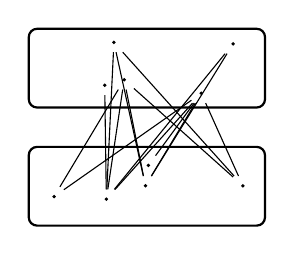
\begin{tikzpicture}[color=black]

\node (rect) at (0,0)[draw,thick,minimum width=3cm, minimum height = 1cm, rounded corners=3pt]{};

\node (rect2) at (0,1.5)[draw,thick,minimum width=3cm, minimum height = 1cm, rounded corners=3pt]{};

\pgfmathsetseed{3}
% \def\z{rand}
\foreach \x in {1,...,5}
{
\filldraw (rand*1.4,rand*.4) circle (0.4pt) node(a\x){};
\filldraw (rand*1.4,1.5+rand*.4) circle (0.4pt) node(b\x){};

}

\foreach \x in {1,...,5}
{
% \ifthenelse{\x > 1}{\draw[dashed] (a\x) -- (u)}{};
\foreach \y in {1,...,\x}
{
\draw (a\x) -- (b\y);
}
}

\end{tikzpicture}
\end{center}
\caption[][1cm]{(left) The complete bipartite graph on $n$ verticies. We divide the graph into independent sets of size $n/2$, then connect each vertex in the upper set to each vertex in the lower set. This produces $(n/2)^2$ edges and no triangles. \label{fig:bipartite}}
\end{figure}


 Then $\pi(n,K_3) \geq \frac{n^2/4}{{n\choose 2}} \to \frac{1}{2}$. On the other hand, $P_3$ achieves 
 \[	
 \pi(3,K_3) = \frac{\ex(3,K_3)}{3} = \frac{2}{3},
 \]
 so by \cref{thm:pi_decreasing},  $\pi(K_3)\leq \frac{2}{3}$.
Thus, we have
\[	
\frac{1}{2}\leq \pi(K_3)\leq \frac{2}{3}.
\]

How do we make a graph with many edges that does not contain any complete subgraphs on $t$ verticies?

We look at $t$ groups of size $\frac{n}{t}$. Then join two verticies if they lie in different groups, but not join them if they lie in the same group.


\begin{figure}
\begin{center}
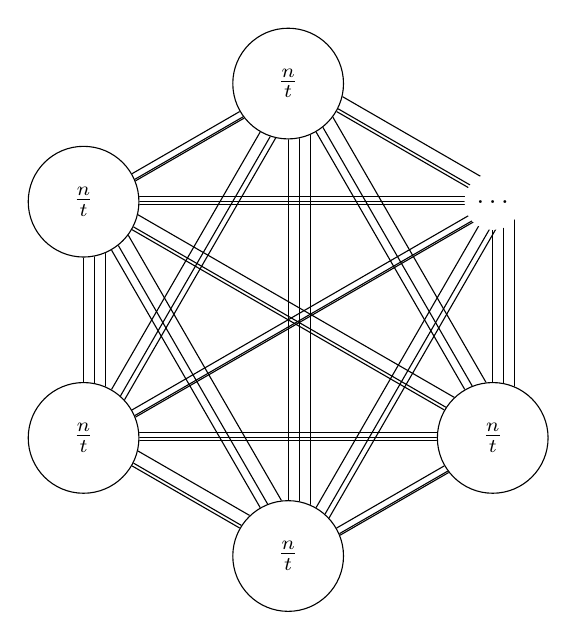
\begin{tikzpicture}
\begin{scope}
% \node[left] at (0,0) {$\circlearrowleft$};


\foreach \y in {1,...,6}
{
\foreach \z in {1,...,\y}
{
\pgfmathsetmacro\myangley{-1*\y*60+90}
\pgfmathsetmacro\myanglez{-1*\z*60+90}
\draw (\myangley:3cm) -- (\myanglez:3cm);
\draw[xshift=4pt,yshift=-1pt] (\myangley:3cm) -- (\myanglez:3cm);
\draw[xshift=8pt,yshift=2pt] (\myangley:3cm) -- (\myanglez:3cm);
}
}
 % do a few by hand
 \pgfmathsetmacro\myangley{-1*3*60+90}
 \pgfmathsetmacro\myanglez{-1*5*60+90}
% \draw (\myangley:3cm) -- (\myanglez:2.9cm);



\foreach \x in {1,...,6}
{
 \pgfmathsetmacro\myangle{-1*\x*60+90}

\ifthenelse{\x > 1}{
\filldraw[white] (\myangle:3cm) circle (20pt);
\draw[black] (\myangle:3cm) circle (20pt) node{$\frac{n}{t}$
};
}{
\filldraw[white] (\myangle:3cm) circle (10pt);
\draw (\myangle:3cm) node[auto]{$\ldots$};
};

}


%  \pgfmathsetmacro\myangle{-1*60+90}
% \draw (\myangle:3cm) node[auto]{$\ldots$};

\end{scope}
\end{tikzpicture}
\end{center}
\caption{The Tur\'an graph on $n$ verticies, in the case that $n$ is divisible by $t$. We partition the graph into $t$ independent subsets of size $\frac{n}{t}$. Then we connect each vertex in each independent subset $A$ to all the verticies in $V(G)\setminus A$.  \label{fig:turan_graph}}
\end{figure}
% Connect each circle to every other circle, several times.


The \defn{Tur\'an graph} $T_t(n)=T$ is a graph with $|V(T)|=n$ such that $V(T)$ is  partitioned into $A_1,\dotsc,A_{t}$ and $v\in A_i$ is adjacent to $u\in A_j$ iff $i\neq j$, and the sizes obey $||A_i| - |A_j|| \leq 1$ for all $i,j$.

Then
\[
\pi(K_t) \geq \lim_{n\to\infty} \frac{|\edges (T_{t-1}(n))|}{{n\choose 2}} = \lim_{n\to\infty} \frac{{n\choose 2} - (t-1){\frac{n}{t-1} \choose 2}}{{n\choose 2}}= 1 - \frac{1}{t-1} = \frac{t-2}{t-1}
\]

\begin{theorem}[\cite{turan1941extremal}] \label{thm:turan}
For every $t\geq 2$, $\pi(K_t) = \frac{t-2}{t-1}$. Moreover,
\[
\ex(n,K_t)\leq \frac{t-2}{t-1} \frac{n^2}{2}.
\]
\end{theorem}
\begin{proof}[Proof by induction on $n$.] 
Note that when $n$ is divisible by $t-1$,
\[
\ex(n,K_t)\geq |\edges (T_{t-1}(n))| = \frac{t-2}{t-1}\frac{n^2}{2}
\]
and equality is acheived.
Base case: for $n < t-1$, then the maximal number of edges (without restriction) is ${n\choose 2}  = \frac{n-1}{n}\frac{n^2}{2}\leq \frac{t-2}{t-1}\frac{n^2}{2}$.

Induction step. Let $n\geq t-1$. We may assume that $K_{t-1}$ is a subgraph of our graph $G$ (where $G$ is a graph on verticies with no $K_t$ subgraph and $|\mathcal{G}| = \ex(n,K_t)$.

Let $U=\{v_1,v_2,\dotsc,v_{t-1}\}$ be the set of verticies of this $K_{t-1}$ subgraph. Then
\[	
 |\edges (G) | = \frac{(t-1)(t-2)}{2} + | \edges (U,V(G)\setminus U)| + |\edges (G\setminus U)|.
 \]
 This is the number of edges within $U$, plus the number of edges with exactly one end in $U$, plus the number of edges not connected to $U$, respectively. See \cref{fig:U_VG-U} for a depiction of this partition.

 % \missingfigure{partition of $G$ into $U$ and $V(G)\setminus U$. $U$ is a complete graph. Put a point $u$ in the latter.}
\begin{marginfigure}
\begin{center}
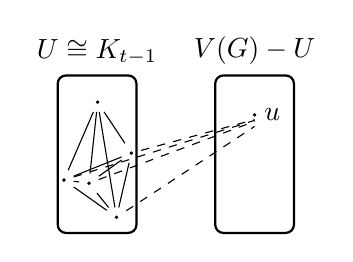
\begin{tikzpicture}
\node (rect) at (0,0)[draw,thick,minimum width=1cm, minimum height = 2cm, rounded corners=3pt,label=above:$U\cong K_{t-1}$]{};

\node (rect2) at (2,0)[draw,thick,minimum width=1cm, minimum height = 2cm, rounded corners=3pt,label=above:$V(G)\setminus U$]{};

\pgfmathsetseed{3}
% \def\z{rand}
\foreach \x in {1,...,5}
{
\filldraw[black] (rand*.5,rand*1) circle (0.4pt) node(a\x){};
}
% \draw (a1) -- (a2);

\filldraw[black] (2,.5) circle (0.4pt) node[right](u){$u$};



\foreach \x in {1,...,5}
{
\ifthenelse{\x > 1}{\draw[dashed] (a\x) -- (u)}{};
\foreach \y in {1,...,\x}
{
\draw (a\x) -- (a\y);
}
}

% \filldraw at (rect2)[draw, fill=black,circle(.4pt),above,label=above:$u$]{};

\end{tikzpicture}
\end{center}
\caption{ Illustation of the partition of $G$ into $V(G)\setminus U \ni u$ and $U$. If $u$ were adjacent to more than $t-2$ notes in $U$, then $U\cup \{u\} \cong K_t$. \label{fig:U_VG-U}}
\end{marginfigure}



 For every $u\in V(G)\setminus U$, the vertex $u$ is adjacent to $\leq t-2$ verticies in $U$ (otherwise $U\cup\{u\}\cong K_t$). So
 \[
 \edges (U,V(G)-U)| \leq (t-2) |V(G)-U| = (t-2)(n-t-1).
 \]

 Moreover,
 \[
 |\edges (G\setminus U)|  \leq \frac{t-2}{t-1}\frac{(n-t+1)^2}{2},
 \]
 by the induction hypothesis. Putting it all together,
 \begin{align*}
 |\edges (G)| &\leq \frac{(t-1)(t-2)}{2} + (t-2)(n-t+1) + \frac{t-2}{t-1}\frac{(n-t+1)^2}{2}\\
 &= \frac{t-2}{2(t-1)} \left( (t-1)^2 + 2(t-1) (n-t+1) + (n-t+1)^2 \right)\\
 &= \frac{t-2}{2(t-1)} n^2.\qedhere
 \end{align*}
\end{proof}
\lect{2}{8}
% \marginnote{Lecture 10: Monday, February 8, 2016.}
We'll provide another proof of Tur\'an's theorem, but first let us introduce some notation. Let 
\[
d(G) = \frac{2|\edges (G)|}{n^2}
\]
be the \defn{density}[density of graph] of $G$; this is the probability that choosing two verticies uniformly at random (with repetition) from $V(G)$ gives an edge. The density $\lambda$ is called the \defn{Lagrangian} of $G$.

Suppose $V(G) = [n]$. Let 
\[
\lambda(G) := \max_{\substack{x_i\geq 0,\\ \sum_{i=1}^n x_i=1}} \sum_{(i,j) \in \edges (G)} x_i x_j.
\]
Then $2\lambda(G)$ is the maximum probability of selecting an edge by independently sampling two verticies taken over all probability distributions on the vertex set. In particular, $2\lambda(G) \geq d(G)$, for every $G$.

\begin{example}
\[
\lambda(K_2) = \max_{\substack{x_1,x_2\geq 0 \\ x_1+x_2=1}} x_1 x_2 =\max_{x_1\geq 0} x_1(1-x_1) = \frac{1}{4},
\]
achieved when $x_1=x_2=\frac{1}{2}$.

\[
\lambda(P_3) = \max_{\substack{x_1,x_2,x_3\geq 0\\ x_1+x_2+x_3}} x_1x_2 + x_2x_3 = \max_{\substack{x_1,x_2,x_3\geq 0\\ x_1+x_2+x_3}} x_2(x_1+x_3)
\]
is still a product of two things which sum to one. So we need $x_2=\frac{1}{2}$ and $x_1+x_3=\frac{1}{2}$. We could take $x_1=x_3=\frac{1}{4}$.
\end{example}

\begin{lemma}
$\lambda(K_t) = \frac{t-1}{2 t}$.
\end{lemma}
\begin{proof}	
The uniform distribution on $|V(K_t)|$ acheives $\frac{t-1}{2t}$, so it is enough to show
\[
\sum_{\substack{1\leq i<j \leq t,\\ x_i\geq 0,\\ \sum_{i=1}^n x_i=1.}} x_i x_j \leq \frac{t-1}{2t}.
\]
But
\[
\sum_{\substack{1\leq i<j \leq t,\\ x_i\geq 0,\\ \sum_{i=1}^n x_i=1.}} 2x_i x_j  = (x_1+x_2+\dotsm + x_t)^2 - \sum_{i=1}^t x_i^2 = 1- \sum_{i=1}^t x_i^2 \quad\boxed{\leq} \quad 1 - \frac{1}{t}
\]
where we need to show the boxed inequality.
Equivalently, we need $\sum_{i=1}^t x_i^2 \geq \frac{1}{t}$ for all $x_i$ as above. But this follows from Jensen's inequality (with the uniform distribution): if $f$ is convex, then
\[
\frac{\sum_{i=1}^n f(x_i)}{n} \geq f \left( \frac{x_1+\dotsm + x_n}{n}\right)
\]
for all $x_1,\dotsc,x_n$. 

Here, we take $f(x)=x^2$, to obtain
\[
\frac{\sum_{i=1}^n x_i^2}{t}\geq \left(\frac{x_1+\dotsm + x_t}{t}\right)^2 = \left( \frac{1}{t} \right)^2. \qedhere
\]
\end{proof}

\begin{theorem} \label{thm:lambda_G}
If $G$ has no $K_t$ subgraph, then $\lambda(G) \leq \lambda(K_{t-1}) = \frac{t-2}{2(t-1)}$.
\end{theorem}
\begin{proof}	
Let $p_G(\bar x) = \sum_{\{i,j\}\in \edges (G)} x_i x_j$. Then
\[
\lambda(G) = \max_{\substack{x_i\geq 0 \\ \sum_i x_i =1}} p_G(\bar x).
\]
Choose maximal $\bar x$ so that $p_G(\bar x) = \lambda(G)$, and $\#\{i: x_i \neq 0\}$ is minimal.
We may assume that in fact $x_i>0$ for all $i$, by throwing away verticies with zero weights.
\begin{claim}
$G$ is complete.
\end{claim}
\begin{remark}
This means the probability distribution was concentrated on a complete subgraph.
\end{remark}
\begin{subproof}[Proof of claim]
Suppose $G$ is not complete. Then there exists $i,j\in V(G)$ non-adjacent. We have
\begin{align*}	
p_G(\bar x) &= x_i \overbrace{\sum_{\substack{k: \\ \{k,i\} \in \mathcal{G}(G)}} x_k}^{C_i} + x_j \overbrace{ \sum_{\substack{k: \\ \{k,j\} \in \mathcal{G}(G)}} x_k}^{C_j} + \overbrace{\sum_{\substack{\{k,\ell\} \in \edges (G):\\ k,\ell \in V(G)\setminus \{i,j\} }} x_k x_\ell}^{b}.
\end{align*}
Assume wlog that $C_j\geq C_i$. Let $\bar x'$ be obtained by setting $x'_i=0$ and $x'+j = x_i + x_j$, and the other $x'_k = x_k$ (for $k\neq j$ and $k\neq i$). Then $p_G(\bar x') = (x_i+x_j) C_j + b \geq x_i C_i + x_j C_j + b = p_G(\bar x)$.

This is a contradiction: $\bar x'$ has more zero values than $\bar x$, but still acheives $\lambda(G)$. But we choose $\bar x$ to have the minimal number of non-zero values.
 % But since $\bar x$ is maximal, we must have $C_i = C_j$.
\end{subproof}
Then $G$ is complete, and so must be of size $t-1$.
\end{proof}

\begin{remark}
 \Cref{thm:lambda_G} proves \cref{thm:turan}.
\end{remark}
\begin{proof}	
\[
\frac{|\edges (G)|}{n^2}=p_G(\frac{1}{n}, \dotsc, \frac{1}{n}) \leq\lambda(G) \leq \frac{t-2}{2(t-1)}.\qedhere
\]
\end{proof}
\lect{2}{10}
% \marginnote{Lecture 11: Wednesday, February 10, 2016.}

Let $K_{1,t}$ be the graph \scalebox{.5}{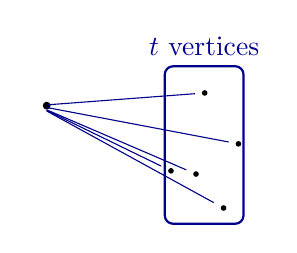
\begin{tikzpicture}[color=DarkBlue]
\node (rect) at (0,0)[draw,thick,minimum width=1cm, minimum height = 2cm, rounded corners=3pt,label=above:{$t$ vertices}]{};

% \node (rect2) at (2,0)[draw,thick,minimum width=1cm, minimum height = 2cm, rounded corners=3pt,label=above:$V(G)\setminus U$]{};

\pgfmathsetseed{3}
% \def\z{rand}
\foreach \x in {1,...,5}
{
\filldraw[black] (rand*.5,rand*1) circle (0.8pt) node(a\x){};
}
% \draw (a1) -- (a2);

\filldraw[black] (-2,.5) circle (1.2pt) node[left](u){};



\foreach \x in {1,...,5}
{
\draw (a\x) -- (u);
}

% \filldraw at (rect2)[draw, fill=black,circle(.4pt),above,label=above:$u$]{};

\end{tikzpicture}}.
Then $\pi(K_{1,t})= 0$, as follows:
We may bound
\[	
\ex(n,K_{1,t}) \leq \frac{(t-1)n}{2}
\]
because every vertex has degree $\leq t-1$ if there is no $K_{t,1}$ subgraph.



Let $K_{2,2}$ be the graph 
\scalebox{.7}{
\begin{tikzpicture}[color=DarkBlue]
\filldraw[black] (0,0) circle (1.2pt) node(a1){};

\filldraw[black] (0,1) circle (1.2pt) node(a2){};


\filldraw[black] (1,0) circle (1.2pt) node(a3){};
\filldraw[black] (1,1) circle (1.2pt) node(a4){};
\draw (a3) -- (a4);

\draw (a1) -- (a2);

\draw (a2) -- (a3);

\draw (a1) -- (a4);



% \foreach \x in {1,...,4}
% {
% \foreach \y in {1,...,2}
% {
% \draw (a\x) -- (a\y);
% }
% }

\end{tikzpicture}}.
If $G$ has no $K_{2,t}$ then it has $\leq (t-1){n\choose 2}$ paths $P_3$ as subgraphs, but if $G$ has $\epsilon {n\choose 2}$ edges, we ``expect'' $\geq \epsilon^2 {n\choose 3}$ paths $P_3$, so if $\epsilon>0$ for large $n$, we get a contradiction.
Thus, $\pi(K_{2,t})=0$.



\begin{theorem}
$\pi(K_{t,t})=0$ for every $t>1$.
\end{theorem}
\begin{remark}
This implies $\pi(H)=0$ for every bipartite graph $H$.
\end{remark}
\begin{proof}	
We need to show that for every $\epsilon>0$ there exists $n_0$ such that if $G$ has no $K_{t,t}$ subgraph, and $n\geq n_0$ verticies, then $|\edges (G)|\leq \epsilon{n\choose 2}$.


Suppose that $|\edges (G)|\geq \epsilon {n\choose 2}$.



\begin{figure}
\begin{center}
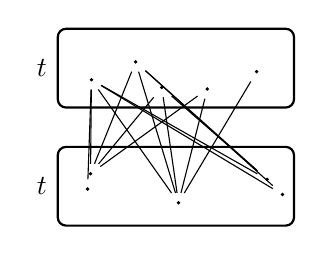
\begin{tikzpicture}[color=black]

\node (rect) at (0,0)[draw,thick,minimum width=3cm, minimum height = 1cm, rounded corners=3pt, label=left:$t$]{};

\node (rect2) at (0,1.5)[draw,thick,minimum width=3cm, minimum height = 1cm, rounded corners=3pt,label=left:$t$]{};

\pgfmathsetseed{4}
% \def\z{rand}
\foreach \x in {1,...,5}
{
\filldraw (rand*1.4,rand*.3) circle (0.4pt) node(a\x){};
\filldraw (rand*1.4,1.5+rand*.3) circle (0.4pt) node(b\x){};

}

\foreach \x in {1,...,5}
{
% \ifthenelse{\x > 1}{\draw[dashed] (a\x) -- (u)}{};
\foreach \y in {1,...,\x}
{
\draw (a\x) -- (b\y);
}
}

\end{tikzpicture}
\end{center}
\caption[][0cm]{Left. The bipartite graph on $n$ verticies. We divide the graph into independent sets of size $n/2$, then connect each vertex in the upper set to each vertex in the lower set. This produces $(n/2)^2$ edges and no triangles. \label{fig:bipartite2}}
\end{figure}

Set
\[
f(G) = \sum_{\{v_1,v_2,\dotsc,v_t\}\subset V(G)^{(t)}} | N(v_1)\cap N(v_2)\dotsm \cap N(v_t)| \leq (t-1){n\choose t}
\]
where $N(v)$ is the set of neighbors of $v$ in $G$: that is, $N(v) = \{u\in V(G): \{u,v\} \in \edges (G) \}$.



We are counting subgraphs of the form
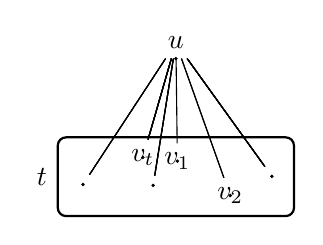
\begin{tikzpicture}[color=black]

\node (rect) at (0,0)[draw,thick,minimum width=3cm, minimum height = 1cm, rounded corners=3pt, label=left:$t$]{};
\filldraw (0,1.5) circle (0.4pt) node[above](u){$u$};

% \node (rect2) at (0,1.5)[draw,thick,minimum width=3cm, minimum height = 1cm, rounded corners=3pt,label=left:$t$]{};

\pgfmathsetseed{3}
% \def\z{rand}
\foreach \x in {1,...,6}
{
\ifthenelse{\x>5}{
\filldraw (rand*1.4,rand*.3) circle (0.4pt) node(a\x){$v_t$};
	
}{
\ifthenelse{\x<3}{

\filldraw (rand*1.4,rand*.3) circle (0.4pt) node(a\x){$v_\x$}; }{
	\filldraw (rand*1.4,rand*.3) circle (0.4pt) node(a\x){};
};
	
};
% \filldraw (rand*1.4,1.5+rand*.3) circle (0.4pt) node(b\x){};

}

\foreach \x in {1,...,6}
{
% \ifthenelse{\x > 1}{\draw[dashed] (a\x) -- (u)}{};
\foreach \y in {1,...,\x}
{
\draw (a\x) -- (u);
}
}

\end{tikzpicture}.

First, note
\[
{m\choose t} \geq \frac{m^t}{t!} - cm^{t-1}
\]
for some constant $c$ depending on $t$ only.

Then,
\begin{align*}	
f(G) &= \sum_{u\in V(G)} {\deg (u) \choose t} \geq \sum_{u\in V(G)} \left( \frac{\deg^t(u)}{t!}- c \deg^{t-1}(u) \right)\\
\intertext{where we've used Jensen's for $t$th powers. Then,}
&\geq \frac{n}{t!} \left( \sum_{u\in V(G)} \frac{\deg(u)}{n} \right)^t - cn^t\\
&\geq \frac{n}{t!} \left( \frac{2 \epsilon {n\choose 2}}{n} \right)^t - cn^t\\
\intertext{Using $2 \epsilon {n\choose 2} \geq \frac{\epsilon}{2}n^2$}
&\geq \frac{n}{t!}\left( \frac{\epsilon}{2}n \right)^t - cn^t\\
& \boxed{>} (t-1) {n \choose t}
\end{align*}
where the boxed inquality yields a contradiction, and holds for large enough $t$.
\end{proof}


If $H$ is not bipartite, is it possible $\pi(H)=0$? No, there exist large ``dense'' graphs with no $H$ subgraph.
For every non-bipartite graph, the Tur\'an density is at least 1/2, for the same reason as $K_3$: it cannot be embedded in a large complete bipartite graph, so these graphs\sidenote[][-2cm]{which have density 1/2} witness this.


Let us consider graphs which are not subgaphs of the Tur\'an graph $T_{3}(n)$ (depicted in \cref{fig:T3}): 
If $H$ is not a subgraph of $T_3(n)$ for any $n$, then $\pi(H)\geq \frac{2}{3}$. Let us generalize.
\begin{marginfigure}[-2cm]
\begin{center}
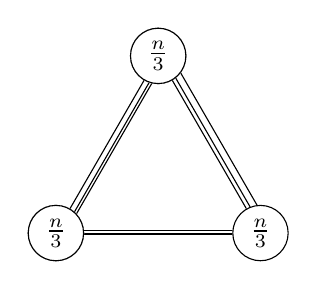
\begin{tikzpicture}[scale=.5]
\begin{scope}
% \node[left] at (0,0) {$\circlearrowleft$};


\foreach \y in {1,...,3}
{
\foreach \z in {1,...,\y}
{
\pgfmathsetmacro\myangley{-1*\y*120+90}
\pgfmathsetmacro\myanglez{-1*\z*120+90}
\draw (\myangley:3cm) -- (\myanglez:3cm);
\draw[xshift=4pt,yshift=-1pt] (\myangley:3cm) -- (\myanglez:3cm);
\draw[xshift=8pt,yshift=2pt] (\myangley:3cm) -- (\myanglez:3cm);
}
}
 % do a few by hand
 \pgfmathsetmacro\myangley{-1*3*120+90}
 \pgfmathsetmacro\myanglez{-1*5*120+90}
% \draw (\myangley:3cm) -- (\myanglez:2.9cm);



\foreach \x in {1,...,6}
{
 \pgfmathsetmacro\myangle{-1*\x*120+90}

\ifthenelse{\x > 1}{
\filldraw[white] (\myangle:3cm) circle (20pt);
\draw[black] (\myangle:3cm) circle (20pt) node{$\frac{n}{3}$
};
}{
\filldraw[white] (\myangle:3cm) circle (10pt);
\draw (\myangle:3cm) node[auto]{$\ldots$};
};

}


%  \pgfmathsetmacro\myangle{-1*60+90}
% \draw (\myangle:3cm) node[auto]{$\ldots$};

\end{scope}
\end{tikzpicture}
\end{center}
\caption{The Tur\'an graph $T_3(n)$.} \label{fig:T3}
\end{marginfigure}


% \begin{definition}%[$k$-coloring, $\chi(G)$]
 We say $c\!\!: V(G) \to [k]$ is a \defn{$k$-coloring} if $c(u)\neq c(v)$ for every $\{u,v\}\in \edges (G)$.

We write $\chi(G)$ for the minimum $k$ such that $G$ admits a $k$-coloring. With this definition in hand, we may formulate the following result.
% \end{definition}
\begin{lemma} \label{lem:min_Tur\'an_density_2graphs}
If $H$ contains an edge,
\[
\pi(H)\geq \frac{\chi(H)-2}{\chi(H)-1}.
\]
\end{lemma}

\begin{proof}	
Let $k = \chi(H)-1$. As $H$ is not $k$-colorable, $H$ is not a subgraph of any Tur\'an graph $T_k(n)$ and so $\pi(H)\geq \lim_{n\to\infty} \frac{|\edges (T_k(n))|}{{n\choose 2}} = \frac{k-1}{k}$.
\end{proof}

\begin{lemma} \label{lem:subgraph_with_min_vertex_degree}
For every $r$, $n_0$, and $\epsilon$, there exists $N$ such that if $G$ is an $r$-graph with $|V(G)| = n\geq N$ and $|\edges (G)|\geq d {n\choose r}$, then $G$ contains a subgraph (sub $r$-graph) $G'$ such that
\[
|V(G')| =n' \geq n_0
\]
and every vertex $v\in V(G')$ belongs to at least $(d - \epsilon) {n' \choose r-1}$ edges.
\end{lemma}
\marginnote{So we can  restrict to a (large) subgraph to obtain a minimal bound on vertex degree, at the cost of $\epsilon$ density. }
\begin{proof}	
Suppose not. Then there exists a vertex $v_1\in V(G)$ such that $v_1$ belongs to at most $(d - \epsilon) {n \choose r-1}$ edges. Delete this vertex to obtain a graph $G_1$ which in turn has a vertex $v_2$ in at most $(d- \epsilon){n-1 \choose r-1}$ edges. Delete this vertex to obtain $G_2$, and continue in the same manner.

We eventually arrive at a graph $G_{n-n_0}$ on $n_0$ verticies. Then
\begin{fullwidth}
\begin{align*}	
d {n \choose r} &\leq |G| \\
&\leq (d -\epsilon){n\choose r-1} + (d- \epsilon) {n-1 \choose r-1} + \dotsm + (d- \epsilon){n_0+1 \choose r-1} + \underbrace{|G_{n-n-0}|}_{\leq {n_0\choose r}}.
\end{align*}
It remains to show that for $n$ large enough (in terms of $n_0,r,\epsilon$)
\[
d {n \choose r} > (d- \epsilon) \left[{n\choose r-1} +  {n-1 \choose r-1} + \dotsm + {n_0+1 \choose r-1}  \right] + {n_0 \choose r}.
\]
But, repeating the Pascal's triangle inequality,
\[
{n\choose r} = {n-1 \choose r-1} + {n-2\choose r-1} + {n-3 \choose r-1} + \dotsm + {r-1 \choose r-1}.
\]
So,
\[
d {n\choose r} = (d - \epsilon) \left( {n-1 \choose r-1} + {n-2\choose r-1} + {n-3 \choose r-1} + \dotsm + {r-1 \choose r-1} \right) + \epsilon {n\choose r}.
\]
\end{fullwidth}

This eliminates most terms; we are left with
\[
\epsilon {n\choose r} \overset{?}{>} (d- \epsilon) {n\choose r-1} + {n_0 \choose r}.
\]
But the polynomial in $n$ on the left has degree $r$, and on the right, degree $r-1$, so for $n\geq N$ with $N$ large enough, we have strict inequality.

\end{proof}

\begin{theorem}[\cite{erdos-stone}]
\[
\pi(H) = \frac{\chi(H)-2}{\chi(H)-1}
\]
for every $2$-graph $H$ with $\chi(H)\geq 2$\marginnote{I.e. $H$ contains an edge.}.
\end{theorem}
\begin{proof}	
\Cref{lem:min_Tur\'an_density_2graphs} gives the lower bound. Now, consider $K_{\underbrace{t,\dotsc,t}_{k \text{ times}}}$ the complete $k$-partite graph with parts of size $t$, as depicted in \cref{fig:Ktttt}.
\begin{figure}
\begin{center}
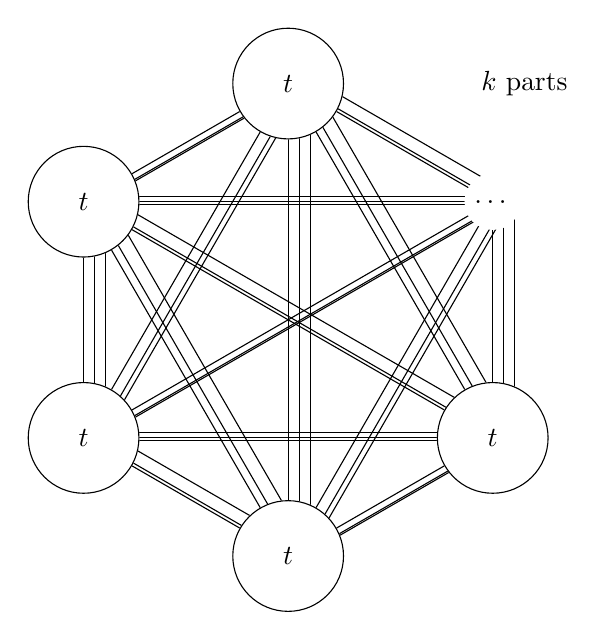
\begin{tikzpicture}
\begin{scope}
% \node[left] at (0,0) {$\circlearrowleft$};


\foreach \y in {1,...,6}
{
\foreach \z in {1,...,\y}
{
\pgfmathsetmacro\myangley{-1*\y*60+90}
\pgfmathsetmacro\myanglez{-1*\z*60+90}
\draw (\myangley:3cm) -- (\myanglez:3cm);
\draw[xshift=4pt,yshift=-1pt] (\myangley:3cm) -- (\myanglez:3cm);
\draw[xshift=8pt,yshift=2pt] (\myangley:3cm) -- (\myanglez:3cm);
}
}
 % do a few by hand
 \pgfmathsetmacro\myangley{-1*3*60+90}
 \pgfmathsetmacro\myanglez{-1*5*60+90}
% \draw (\myangley:3cm) -- (\myanglez:2.9cm);



\foreach \x in {1,...,6}
{
 \pgfmathsetmacro\myangle{-1*\x*60+90}

\ifthenelse{\x > 1}{
\filldraw[white] (\myangle:3cm) circle (20pt);
\draw[black] (\myangle:3cm) circle (20pt) node{$t$
};
}{
\filldraw[white] (\myangle:3cm) circle (10pt);
\draw (\myangle:3cm) node[auto]{\ldots};
};

}
\draw (3,3) node[auto]{$k$ parts};


%  \pgfmathsetmacro\myangle{-1*60+90}
% \draw (\myangle:3cm) node[auto]{$\ldots$};

\end{scope}
\end{tikzpicture}
\end{center}
\caption{An illustration of $K_{tt\dotsm  t}$, where there are $k$ $t$'s in the subscript. This means we have $k$ independent sets of size $t$, and each vertex of each independent set is connected to all the vertices in all the other sets.  \label{fig:Ktttt}}
\end{figure}


For every $t$,
\[	
\pi(K_{t,\dotsc,t}) \leq \frac{k-2}{k-1}
\]
by induction on $k$. Suppose for some $k$, and some $t$,
\[	
\pi(K_{\underbrace{t,\dotsc,t}_{k \text{ times}}}) \geq \frac{k-2}{k-1} + \epsilon.
\]
for $\epsilon>0$. It is enough to show that for every graph $G$ with $n$ vertices such that
\[	
|\edges (G)| \geq \left( \frac{k-2}{k-1}+ \epsilon \right) {n\choose 2},
\]
we must have that $G$ contains $K_{\underbrace{t,\dotsc,t}_{k \text{ times}}}$.

By \cref{lem:subgraph_with_min_vertex_degree} we may assume that every vertex of $G$ has degree
\[	
\geq \left(  \frac{k-2}{k-1} + \frac{\epsilon}{2} \right)n.
\]
By the induction hypothesis, $G$ contains $K_{\underbrace{s,\dotsc,s}_{k-1 \text{ times}}}$ for every $s$. We will choose a particular $s$ depending only on $k$ and $\epsilon$, which we will specify later.

It suffices to prove that if $n$ is large compared to $s,k, \epsilon$, and $s$ is large compared to $k, t$ and $\epsilon$, and $G$ is a graph with $n$ vertices, and each vertex has degree at least $\left(  \frac{k-2}{k-1} + \frac{\epsilon}{2} \right)n$ , and $G$ contains a complete $k-1$-partite subgraph with $s$ vertices in each part, then $G$ contains a complete $k$-partite subgraph with $t$ vertices.
\lect{2}{15}
% \marginnote{Lecture 12: Monday, February 15, 2016.}

Let $A_1,A_2,\dotsc,A_{k-1} \subset V(G)$ with $|A_i| = s$ such that every vertex of $A_i$ is adjacent to every vertex of $A_j$ when $i\neq j$ \marginnote{Such a group of sets is simply $K_{\underbrace{s,\dotsc,s}_{k-1 \text{ times}}}$ and exists by the induction hypothesis.}
Let $U = A_1\cup \dotsc \cup A_{k-1}$ and let $W$ be the set of verticies in $V(G)$ which have $\geq t$ neighbors in each $A_i$.

\begin{figure}
\begin{center}
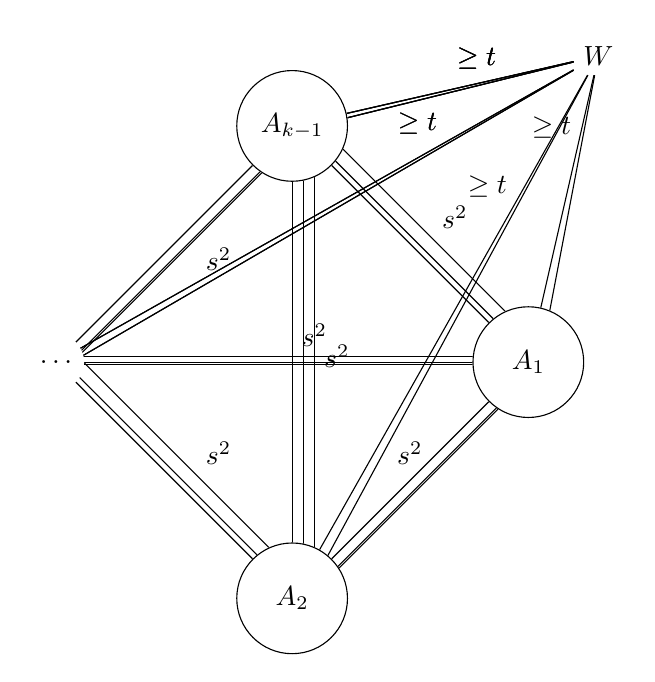
\begin{tikzpicture}
\begin{scope}
% \node[left] at (0,0) {$\circlearrowleft$};

\def\n{4}
\def\radius{.6}
\def\rotation{90}

\def\deg{360/\n}
\pgfmathsetmacro\nminusone{\n-1}

 \pgfmathsetmacro\myangle{-1*.5*\deg+\rotation}

\filldraw[white] (\myangle:5.5cm) circle (10pt);
\draw (\myangle:5.5cm) node[auto](w){$W$};


% do first one
\pgfmathsetmacro\myangley{-1*\deg+\rotation}
\draw (\myangley:3cm) -- (w);
\draw[xshift=4pt,yshift=-1pt] (\myangley:3cm) -- (w) node[near end,auto]{$\geq t$};

% do the rest
\foreach \y in {2,...,\n}
{
\pgfmathsetmacro\yminusone{\y-1}

\foreach \z in {1,...,\yminusone}
{
\pgfmathsetmacro\myangley{-1*\y*\deg+\rotation}
\pgfmathsetmacro\myanglez{-1*\z*\deg+\rotation}
\draw (\myangley:3cm) -- (\myanglez:3cm);
\draw[xshift=4pt,yshift=-1pt] (\myangley:3cm) -- (\myanglez:3cm);
\draw[xshift=8pt,yshift=2pt] (\myangley:3cm) -- (\myanglez:3cm) node[midway,auto]{$s^2$};


\draw (\myangley:3cm) -- (w);
\draw[xshift=4pt,yshift=-1pt] (\myangley:3cm) -- (w) node[near end,auto]{$\geq t$};

}
}
 % do a few by hand
 % \pgfmathsetmacro\myangley{-1*3*120+90}
 % \pgfmathsetmacro\myanglez{-1*5*120+90}
% \draw (\myangley:3cm) -- (\myanglez:2.9cm);



\foreach \x in {1,...,\n}
{
 \pgfmathsetmacro\myangle{-1*\x*\deg+\rotation}

\ifthenelse{\x = \nminusone}{
\filldraw[white] (\myangle:3cm) circle (10pt);
\draw (\myangle:3cm) node[auto]{$\ldots$};
}{
\ifthenelse{\x = \n}{
\filldraw[white] (\myangle:3cm) circle (20pt);
\draw[black] (\myangle:3cm) circle (20pt) node{$A_{k-1}$};
}{
\filldraw[white] (\myangle:3cm) circle (20pt);
\draw[black] (\myangle:3cm) circle (20pt) node{$A_\x$};
}
};

}
\end{scope}
\end{tikzpicture}
\end{center}
\end{figure}
Now, we wish to show $w:= |W|$ is large. First,
\begin{align*}	
\left( \frac{k-2}{k-1}+ \epsilon \right)n(k-1)s &\leq  \sum_{v\in U}\deg(v) \leq \sum_{v\in V(G)} |N(v)\cap U|\\
&\leq \underbrace{w s(k-1)}_{\text{from verticies in }W} + \underbrace{(n-w) (s(k-2)+t)}_{\text{from verticies not in }W}\\
% &= wsn - ws + ns - n(k-2) + nt - ws + w(k-2) - wt\\
% &= wsn - ws + ns - nk + 2n + nt -ws +wk - 2w - wt\\
((k-2) + \epsilon (k-1)) n s &\leq ns (k-2) + nt + w(s-t)
\end{align*}
If we choose $s$ such that $\epsilon (k-1) s -t \geq 1$, then
\[
% &= nsk - 2ns + nt + ws - wt
n \leq n( \epsilon (k-1)s - t) \leq w (s-t) \leq ws.
\]
Then $W\geq \frac{n}{s}$. For each $v\in W$ let $(B_1^v,B_2^v,\dotsc,B_{k-1}^v)$ be the sets of neighbors of $v$ of size $t$ such that $B_i \subset A_i$. There are ${s \choose t}^{k-1}$ choices of these sequences of neighbors, so if $w > \underbrace{s(k-1)}_{\text{vertices in }U}+ (t-1) {s \choose t}^{k-1}$ \marginnote{So $|W\setminus U| \geq |W| - |U| \geq (t-1) {s \choose t}^{k-1}$.} then by pigeonhole principle, there exists $t$  entries in $W\setminus U$ which have the same $t$ neighbors in each of the $A_i$, as desired.\qedhere

\marginnote{The entries in $W\setminus U$ don't need to be independent, because we just need a subgraph, so we can just not include those edges in our subgraph.}


\end{proof}
% section turian_type_problems (end)
\begin{fullwidth}
\printbibliography[segment=\therefsegment,heading=subbibliography]
\end{fullwidth}


\clearpage
\newrefsegment
%!TEX root = ../CombinatoricsNotes.tex

\section{Hypergraph Tur\'an Problems} % (fold)
\label{sec:hypergraph_turan_problems}
\marginnote{These are typically extremely difficult.}
Let $K_4^{(3)}$ be a complete 3-graph on $4$ vertices: 
\[
K_4^{(3)}=\{ \{a,b,c\},\{a,b,d\},\{a,c,d\},\{b,c,d\}\}.
\]
Then $\pi(K_4^{(3)})$ is not known\sidenote{An old and important problem.}.

Consider the generalized triangle $T_3 = \{D_1,D_2,D_3\}$ where $D_1 = \{1,2,3\}$, $D_2 = \{1,2,4\}$, and $D_3 = \{3,4,5\}$; see \cref{fig:T3}. 
\begin{marginfigure}[1cm]
\begin{center}
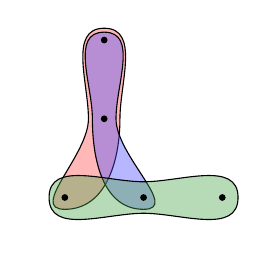
\begin{tikzpicture}[color=black]
\def\radius{1}


\node (a3) at (0,0){};
\node (a4) at (1,0){};
\node (a5) at (2,0) {};
\node (a2) at (.5,1) {};
\node (a1) at (.5,2) {};




\begin{scope}[fill opacity=.4]

  \filldraw[fill=red!70] ($(a1) + (0,0.15)$) 
        to[out=0,in=90] ($(a2)+(.2,0)$)
        to[out=270,in=0] ($(a3) + (0,-.15)$)
        % to[out=180,in=0] ($(a3) + (0,-.1)$)
        to[out=180,in=270] ($(a2)+(-0.2,0)$)
        to[out=90,in=180] ($(a1)+(0,.15)$);

  \filldraw[fill=blue!70] ($(a1) + (0,0.1)$) 
        to[out=0,in=90] ($(a2)+(.15,0)$)
        to[out=270,in=0] ($(a4) + (0,-.15)$)
        % to[out=180,in=0] ($(a4) + (0,-.1)$)
        to[out=180,in=270] ($(a2)+(-0.15,0)$)
        to[out=90,in=180] ($(a1)+(0,.1)$);

   \filldraw[fill=green!70] ($ (a3) + (-.2,0) $)
   		to[out=90, in=180] ($ (a4) + (0,.2) $)
   		to[out=0, in=90] ($ (a5) + (.2,0) $)
   		to[out=270, in=0] ($ (a4) + (0,-.2) $)
   		to[out=180, in=270] ($ (a3) + (-.2,0) $);


\end{scope}

\filldraw (a3) circle (\radius pt);
\filldraw (a4) circle (\radius pt);
\filldraw (a5) circle (\radius pt);
\filldraw (a2) circle (\radius pt);
\filldraw (a1) circle (\radius pt);

\end{tikzpicture}
\end{center}
\caption{An illustration of $T_3$, numbered from top to bottom, left to right. Then $D_1$ is in red, $D_2$ in blue, and $D_3$ in green. \label{fig:T3}}
\end{marginfigure}


 We will say $C: V(H) \to [k]$ is a \defn{strong $k$-coloring} if $c(v)\neq c(u)$ whenever $u$ and $v$ belong to an edge of $H$.
 $\chi_s(H) = \min k$ such that $H$ can be strongly $k$-colored.

In this language,  $\chi_s(T_3)=4$, so $T_3$ is not a subgraph of any strongly $3$-colorable graph. 
% Then density is $1\cdot\frac{2}{3}\cdot \frac{1}{3}=\frac{2}{9}$, so $\pi(T_3)\geq \frac{2}{9}$.
There exist strongly $3$-colorable graphs with density $2/9$, so $\pi(T_3)\geq 2/9$. We will show $\pi(T_3)=\frac{2}{9}$.

First, we will define an analog to the 2-graph Lagrangian defined in the previous section.
Let $H$ be an $r$-graph, $V(H) = [n]$. For $\bar x = (x_1,x_2,\dotsc,x_n)\in \R^n$, let 
\[
 P_H(\bar x) = \sum_{e\in H} \prod_{i\in e} x_i.
 \] If $x_i\geq 0$ and $\sum_i x_i = 1$, i.e. $\bar x$ corresponds to a probability distribution on $|V(H)|$, then $\frac{1}{r!}P_H(\bar x)$ is the probability that selecting $r$ verticies independently at random produces an edge. The \defn{hypergraph Lagrangian} is $\lambda(H) := \max P_H(\bar x)$ where the maximum is taken over all $\bar x \geq 0$, $\sum_{i\in[n]}x_i = 1$.

\begin{lemma} \label{lem:6p1}
Let $H$ be an $r$-graph with $|V(H)|=n$. Then
\begin{enumerate}
	\item\label{lem:6p1p1}$\lambda(H)\geq \frac{|\edges (H)|}{n^r} = P_H(\frac{1}{n}\cdot \bar 1)$.
\end{enumerate}
	Now, let $\bar x\geq 0$, $\sum_{i\in[n]}x_i = 1$ be such that $\lambda(H) = P_H(\bar x)$. Moreover, assume for every such $\bar x$, we have  $i\in[n]$, $x_i > 0$. Then,
\begin{enumerate}\setcounter{enumi}{1}
	\item\label{lem:6p1p2} For all $u,v\in V(H)$ there exists $e\in \edges (H)$  containing both $u$ and $v$, and \marginnote{That is, $H$ covers all pairs.}
	\item\label{lem:6p1p3} $\frac{\partial }{\partial x_i} P_H(\bar x) = r \cdot \lambda(H)$.

\end{enumerate}

\end{lemma}
\begin{proof}	
\begin{enumerate}
	\item This is immediate.
	\item Suppose no edge contains $u$ and $v$. Then 
	\[
	 P_H(\bar x) = C_u x_u + C_v x_v + b
	 \] 
	 where $C_u,C_v, b$ do not depend on $x_u$ and $x_v$. As in the graph case, assume $C_u\geq C_v$. Let $x'$ be such that
	 \[
	 x_u'  = x_u + x_v, \qquad x_v' = 0, \qquad x'_w = x_w \text{ for }w\neq \{u,v\}
	 \]
	 then $P_H(\bar x') \geq P_H(\bar x) = \lambda (H)$, contradicting the conditions on $H$. \marginnote{Namely that every extremal $\bar x$ has $x_v>0$.}
	 \item Lagrange multiplier principle: let $\bar x$ be a local maximum of $f(\bar x)$ such that $g(\bar x)=0$\sidenote{A constraint.}. Then 
	 \[
	 \left( \frac{\partial f}{\partial x_1}, \frac{\partial f}{\partial x_2},\dotsc, \frac{\partial f}{\partial x_n} \right) = \nabla f, \text{ and } \left( \frac{\partial g}{\partial x_1}, \dotsc, \frac{\partial g}{\partial x_n} \right) = \nabla g
	 \]
	 are colinear. Applied to $f = P_H$ and $g = \sum x_i -1$, this principle implies
	 \[
	 C = \frac{\partial P_H}{\partial x_i} = \frac{\partial P_H}{\partial x_j}
	 \]
	 for all $i,j$. Then
	 \begin{align*}	
	 \sum_{i=1}^n x_i \frac{\partial P_H}{\partial x_i} &= \sum_{i=1}^n x_i \frac{\partial}{\partial x_i}  \sum_{e\in H} \prod_{j\in e} x_j\\
	 &=\sum_{i=1}^n \sum_{e\in H} x_i   \delta_{i\in e}\prod_{j\in e\setminus \{i\}} x_j\\
	 &=\sum_{e\in H} \sum_{i=1}^n \delta_{i\in e}  \prod_{j\in e} x_j\\
	 &= \sum_{e\in H} r \prod_{j\in e} x_j
	 =r P_H(\bar x).
	 \end{align*}
	 \marginnote{This argument works for all multilinear polynomials homogeneous of degree $r$.}
	 Then
	 \[
	 C = \sum_{i=1}^n x_i C = r \lambda (H).
	 \]
\end{enumerate}
\end{proof}


Define a $3$-graph $K_4^- = \{ \{1,2,3\},\{1,2,4\},\{1,3,4\}\}$; see \cref{fig:K4minus}.
\begin{marginfigure}
\begin{center}
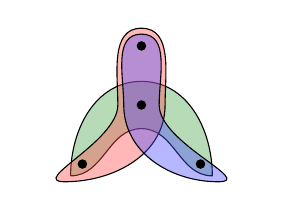
\begin{tikzpicture}[color=black,scale=1.5]
\def\radius{1}


\node (a3) at (0,0){};
\node (a4) at (1,0){};
\node (a2) at (.5,1) {};
\node (a1) at (.5,.5) {};

\begin{scope}[fill opacity=.4]


   \filldraw[fill=green!70] ($ (a3) + (-.1,-.1) $)
   		to[out=90, in=180] ($ (a1) + (0,.2) $)
   		to[out=0, in=90] ($ (a4) + (.1,-.10) $)
   		to[out=180, in=0] ($ (a1) + (0,-.2) $)
   		to[out=180, in=0] ($ (a3) + (-.1,-.1) $);
  \filldraw[fill=red!70] ($(a2) + (0,0.15)$) 
        to[out=0,in=90] ($(a1)+(.2,0)$)
        to[out=270,in=0] ($(a3) + (-.15,-.15)$)
        % to[out=180,in=0] ($(a3) + (0,-.1)$)
        to[out=180,in=270] ($(a1)+(-0.2,0)$)
        to[out=90,in=180] ($(a2)+(0,.15)$);


  \filldraw[fill=blue!70] ($(a2) + (0,0.1)$) 
        to[out=0,in=90] ($(a1)+(.15,0)$)
        to[out=270,in=0] ($(a4) + (.15,-.15)$)
        % to[out=180,in=0] ($(a3) + (0,-.1)$)
        to[out=180,in=270] ($(a1)+(-0.15,0)$)
        to[out=90,in=180] ($(a2)+(0,.1)$);

\end{scope}

\filldraw (a3) circle (\radius pt);
\filldraw (a4) circle (\radius pt);
\filldraw (a2) circle (\radius pt);
\filldraw (a1) circle (\radius pt);

\end{tikzpicture}
\end{center}
\caption{An illustration of $K_4^-$. \label{fig:K4minus}}
\end{marginfigure}

\begin{lemma} \label{lem:noT3noK4minus}
Let $H$ be a $3$-graph (with at least one edge) with no $T_3$ subgraph and no $K_4^-$ subgraph, then $\lambda(H) = \frac{1}{27} = \frac{2}{9}\frac{1}{3!}$.
\end{lemma}
\begin{proof}	
We may assume that any vector $\bar x$ maximizer of $P_H(\bar x)$ such that $\bar x \geq 0$, $\sum x_i = 1$ has no zero components\sidenote{Otherwise, remove those vertices; this doesn't change $P_H(\bar x)$ or $\lambda(H)$.}. Then by \cref{lem:6p1}(\ref{lem:6p1p2}), $H$ covers pairs. In fact, as $H$ contains no $T_3$ or $K_4^-$, every pair in $H$ is covered by exactly one edge. This argument is illustrated in \cref{fig:exactlyoneedge}.
\begin{marginfigure}
\begin{center}
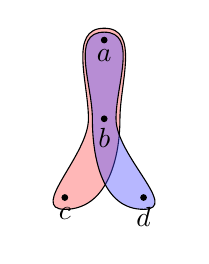
\begin{tikzpicture}[color=black]
\def\radius{1}


\node (a3) at (0,0){};
\node (a4) at (1,0){};
% \node (a5) at (2,0) {};
\node (a2) at (.5,1) {};
\node (a1) at (.5,2) {};




\begin{scope}[fill opacity=.4]

  \filldraw[fill=red!70] ($(a1) + (0,0.15)$) 
        to[out=0,in=90] ($(a2)+(.2,0)$)
        to[out=270,in=0] ($(a3) + (0,-.15)$)
        % to[out=180,in=0] ($(a3) + (0,-.1)$)
        to[out=180,in=270] ($(a2)+(-0.2,0)$)
        to[out=90,in=180] ($(a1)+(0,.15)$);

  \filldraw[fill=blue!70] ($(a1) + (0,0.1)$) 
        to[out=0,in=90] ($(a2)+(.15,0)$)
        to[out=270,in=0] ($(a4) + (0,-.15)$)
        % to[out=180,in=0] ($(a4) + (0,-.1)$)
        to[out=180,in=270] ($(a2)+(-0.15,0)$)
        to[out=90,in=180] ($(a1)+(0,.1)$);

   % \filldraw[fill=green!70] ($ (a3) + (-.2,0) $)
   % 		to[out=90, in=180] ($ (a4) + (0,.2) $)
   % 		to[out=0, in=90] ($ (a5) + (.2,0) $)
   % 		to[out=270, in=0] ($ (a4) + (0,-.2) $)
   % 		to[out=180, in=270] ($ (a3) + (-.2,0) $);


\end{scope}

\filldraw (a3) circle (\radius pt) node[below]{$c$};
\filldraw (a4) circle (\radius pt) node[below]{$d$};
% \filldraw (a5) circle (\radius pt) node[below]{$e$};
\filldraw (a2) circle (\radius pt) node[below]{$b$};
\filldraw (a1) circle (\radius pt) node[below]{$a$};

\end{tikzpicture}
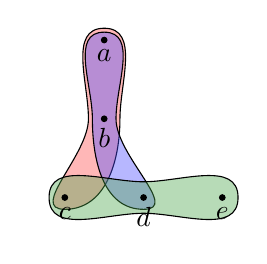
\begin{tikzpicture}[color=black]
\def\radius{1}


\node (a3) at (0,0){};
\node (a4) at (1,0){};
\node (a5) at (2,0) {};
\node (a2) at (.5,1) {};
\node (a1) at (.5,2) {};




\begin{scope}[fill opacity=.4]

  \filldraw[fill=red!70] ($(a1) + (0,0.15)$) 
        to[out=0,in=90] ($(a2)+(.2,0)$)
        to[out=270,in=0] ($(a3) + (0,-.15)$)
        % to[out=180,in=0] ($(a3) + (0,-.1)$)
        to[out=180,in=270] ($(a2)+(-0.2,0)$)
        to[out=90,in=180] ($(a1)+(0,.15)$);

  \filldraw[fill=blue!70] ($(a1) + (0,0.1)$) 
        to[out=0,in=90] ($(a2)+(.15,0)$)
        to[out=270,in=0] ($(a4) + (0,-.15)$)
        % to[out=180,in=0] ($(a4) + (0,-.1)$)
        to[out=180,in=270] ($(a2)+(-0.15,0)$)
        to[out=90,in=180] ($(a1)+(0,.1)$);

   \filldraw[fill=green!70] ($ (a3) + (-.2,0) $)
   		to[out=90, in=180] ($ (a4) + (0,.2) $)
   		to[out=0, in=90] ($ (a5) + (.2,0) $)
   		to[out=270, in=0] ($ (a4) + (0,-.2) $)
   		to[out=180, in=270] ($ (a3) + (-.2,0) $);


\end{scope}

\filldraw (a3) circle (\radius pt) node[below]{$c$};
\filldraw (a4) circle (\radius pt) node[below]{$d$};
\filldraw (a5) circle (\radius pt) node[below]{$e$};
\filldraw (a2) circle (\radius pt) node[below]{$b$};
\filldraw (a1) circle (\radius pt) node[below]{$a$};

\end{tikzpicture}

\end{center}
\caption{\emph{Left:} A depiction of two edges covering the pair $\{a,b\}$, yielding two distinct points $c$ and $d$. \emph{Right:} some edge must cover $\{c,d\}$; this edge has a third point $e$. If $e\in \{a,b\}$, then we have a $K_4^-$ subgraph; otherwise, a $T_3$ subgraph. \label{fig:exactlyoneedge}}
\end{marginfigure}
Let $|V(H)|=n$. Then, using \cref{lem:6p1}(\ref{lem:6p1p3}), we have
\[
3 n \lambda (H) = \sum_{i=1}^n \frac{\partial}{\partial x_i} P_H(\bar x) = \sum_{\{i,j\}\in [n]^{(2)}} x_i x_j \leq \lambda(K_n) = \frac{1}{2}\frac{n-1}{n}.
\]
Then
\[
\lambda(H) \leq \frac{1}{6} \frac{n-1}{n^2} \leq\frac{1}{6}\cdot\frac{2}{9}=\frac{1}{27},
\]
taking $n=3$ and using that $\frac{n-1}{n^2}$ is decreasing for $n>2$. On the other hand, by \cref{lem:6p1}(\ref{lem:6p1p1}), any $3$-graph $H$ with an edge has
\[
\lambda(H) \geq \frac{|\edges (H)|}{n^r} \geq  \frac{1}{3^3}=\frac{1}{27}.\qedhere
\]
\end{proof}

% \marginnote[1cm]{Lecture 13: Wednesday, February 17, 2016.}
\lect{2}{17}
\begin{theorem}[\cite{Erdos-Simon1983}] \label{thm:erdos_simonvits} 
Assume $\F = \{F_1,\dotsc,F_k\}$ is a family of $r$-graphs. Then for every $\epsilon$, there exists $\delta >0$ and $n_0$ such that if $G$ is an $r$-graph on $n\geq n_0$ vertices with $|\edges (G)| \geq (\pi(\F) + \epsilon) {n \choose r}$, then for some $1\leq i \leq k$, then $G$ contains at least $\delta {n\choose |V(F_i)|}$ copies of $F_i$.
\end{theorem}
We will  apply this result to $T_3$ before proving it.
\begin{theorem}
\[
\pi(T_3) = \frac{2}{9}.
\]
\end{theorem}
\begin{proof}	
Suppose $\pi(T_3) = \frac{2}{9}+ 2 \epsilon$ for some $\epsilon>0$. Let $\F = \{T_3, K_4^-\}$. Then $\pi(\F) = \frac{2}{9}$ by \cref{lem:noT3noK4minus}. Let $\delta,n_0$ satisfy \cref{thm:erdos_simonvits} for these $\F,\epsilon$. Let $G$ have $|V(G)| = n > n_0$, $|\edges (G)| \geq ( \frac{2}{9}+ \epsilon) {n \choose 3}$. We will show that (if $n$ is large enough) $G$ contains $T_3$. This will finish the proof. 

If not, then by \cref{thm:erdos_simonvits}, $G$ contains $\geq \delta {n\choose 4}$ copies of $K_4^-$. Then there exists a pair $a,b\in V(G)$ such that $a,b$ belong to $\geq \frac{\delta {n\choose 4}}{{n \choose 2}} \geq \frac{\delta}{12}n^2$ copies of $K_4^-$ in which neither $a$ nor $b$ belong to all three edges\sidenote{Why? Pigeonhole argument: we are distributing  $\delta {n\choose 4}$ copies of $K_4^-$ among ${n\choose 2}$ pairs of verticies; some pair of verticies must end up with at least $\frac{\delta {n\choose 4}}{{n \choose 2}}$ copies of $K_4^-$.}.
% \understand

Let one such copy of $K_4^-$ be that of \cref{fig:K4minuslabelled}. Then $\{a,b\}$ must belong to an edge which contains  neither $c$ nor $d$ (otherwise $\{a,b\}$ is only in two edges: $\{a,b,c\}$ and $\{a,b,d\}$).
Let $\{a,b,e\}$ be such an edge. Then $\{\{a,c,d\},\{b,c,d\},\{a,b,e\}\}$ is $T_3$ as desired. \qedhere

\begin{marginfigure}
\begin{center}
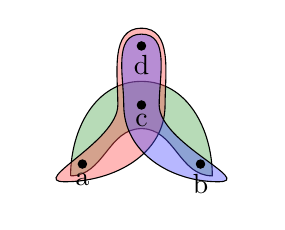
\begin{tikzpicture}[color=black,scale=1.5]
\def\radius{1}


\node (a3) at (0,0){};
\node (a4) at (1,0){};
\node (a2) at (.5,1) {};
\node (a1) at (.5,.5) {};

\begin{scope}[fill opacity=.4]


   \filldraw[fill=green!70] ($ (a3) + (-.1,-.1) $)
   		to[out=90, in=180] ($ (a1) + (0,.2) $)
   		to[out=0, in=90] ($ (a4) + (.1,-.10) $)
   		to[out=180, in=0] ($ (a1) + (0,-.2) $)
   		to[out=180, in=0] ($ (a3) + (-.1,-.1) $);
  \filldraw[fill=red!70] ($(a2) + (0,0.15)$) 
        to[out=0,in=90] ($(a1)+(.2,0)$)
        to[out=270,in=0] ($(a3) + (-.15,-.15)$)
        % to[out=180,in=0] ($(a3) + (0,-.1)$)
        to[out=180,in=270] ($(a1)+(-0.2,0)$)
        to[out=90,in=180] ($(a2)+(0,.15)$);


  \filldraw[fill=blue!70] ($(a2) + (0,0.1)$) 
        to[out=0,in=90] ($(a1)+(.15,0)$)
        to[out=270,in=0] ($(a4) + (.15,-.15)$)
        % to[out=180,in=0] ($(a3) + (0,-.1)$)
        to[out=180,in=270] ($(a1)+(-0.15,0)$)
        to[out=90,in=180] ($(a2)+(0,.1)$);

\end{scope}

\filldraw (a3) circle (\radius pt) node[below] {a};
\filldraw (a4) circle (\radius pt) node[below] {b};
\filldraw (a2) circle (\radius pt) node[below]{d};
\filldraw (a1) circle (\radius pt) node[below]{c};

\end{tikzpicture}
\end{center}
\caption{A labelled illustration of $K_4^-$. \label{fig:K4minuslabelled}}
\end{marginfigure}

\end{proof}


\begin{proof}[Proof of \cref{thm:erdos_simonvits}]
Let us only consider the case $\F=\{F\}$ for simplicity. Let $n'$ be such that every graph $G$ on $n'$ vertices with $|\edges(G)|\geq (\pi (\F) + \frac{\epsilon}{2}) {n' \choose r}$ contains $F$; such an $n'$ exists by the definition of limit. We will choose $n_0$ appropriately large compared to $n'$.
% \unsure{Can't we have any $n_0\geq n'$?}
\begin{claim}
At least $\frac{\epsilon}{2}{n\choose n'}$ subgraphs of $G$ on $n'$ vertices have at least $(\pi(F) + \frac{\epsilon}{2} ) {n' \choose r}$ edges, and thus have a copy of $F$.
\end{claim}
\begin{subproof}[Proof of claim.]
Suppose not. (Let $V(G)=[n]$). Then
\begin{gather*}
|\edges(G)| \underbrace{{n-r \choose n'-r}}_{\substack{\text{\# of $n'$-element sets}\\\text{containing an edge}}} = \sum_{X\in [n]^{(n')}} \underbrace{| \edges (G|X)|}_{\text{edges in $G$ restricted to $X$}}
\end{gather*}
\begin{fullwidth}
By our assumption,
\begin{align*}
\sum_{X\in [n]^{(n')}} | \edges (G|X)| &= \sum_{X:\, |\edges (X)| \geq ( \pi(F) + \frac{\epsilon}{2}) {n' \choose r}) }\edges (G|X) + \sum_{X:\, |\edges (X)| < ( \pi(F) + \frac{\epsilon}{2}) {n' \choose r}) }\edges (G|X) \\
&\leq\frac{\epsilon}{2} {n \choose n'}\underbrace{{n' \choose r}}_{\text{maximal \# edges}} + (1 - \frac{\epsilon}{2}){n \choose n'} (\pi(\F) + \frac{\epsilon}{2}){n' \choose r}
\end{align*}
On the other hand, $|\edges (G)| \geq ( \pi(F) + \epsilon) {n \choose r})$, so we have
\[
( \pi(F) +\epsilon) {n \choose r}{n-r \choose n'-r}\leq \frac{\epsilon}{2} {n \choose n'}{n' \choose r} + (1 - \frac{\epsilon}{2}){n \choose n'} (\pi(\F) + \frac{\epsilon}{2}){n' \choose r}.
\]
\end{fullwidth}
But, by \cref{eq:binomial_identity_boxes}, we have ${n \choose r}{n-r \choose n'-r}  ={n \choose n'}{n' \choose r} $, so
\begin{gather*}	
\pi(F) + \epsilon \leq \frac{\epsilon}{2} + (1- \frac{\epsilon}{2}) (\pi(F) + \frac{\epsilon}{2})\\
\pi(F)+\frac{\epsilon}{2} \leq \pi(F) + \frac{\epsilon}{2} - \frac{\epsilon}{2}\pi(F) - \frac{\epsilon^2}{4}\\
0 \leq - \frac{\epsilon}{2}\pi(F) - \frac{\epsilon^2}{4}
\end{gather*}
which is a contradiction, since $\pi(F)\geq 0$.
\end{subproof}
So by the choice of $n'$ each of these subgraphs contains $F$. Suppose $G$ contains $k$ copies of $F$, and $v = |V(F)|$. Then each of these copies is counted in ${n-v \choose n'-v}$ many $n'$-vertex subgraphs. So, by our claim, $k {n-v \choose n'-v} \geq \frac{\epsilon}{2}{n\choose n'}$. Then,
\[
k\geq \frac{\epsilon}{2} \frac{{n\choose n'}}{{n-v\choose n'-v}} = \frac{\epsilon}{2} \frac{{n\choose v}}{{n' \choose v}} = \frac{\frac{\epsilon}{2}}{{n' \choose v}} {n \choose v} = \delta {n \choose v}
\]
where $\delta := \frac{\frac{\epsilon}{2}}{{n' \choose v}}$, and we've used \cref{eq:binomial_identity_boxes} again.
\end{proof}


\subsection{Tur\'an density of Fano plane.} \marginnote{Finite projective geometry}
The Fano plane $F_7$ is the 3-graph on vertices $\Z_2^3 \setminus \{(0,0,0)\}$, i.e. triples of 0s and 1s not all zero. We declare $\{x,y,z\}$ to be an edge of $F_7$ if $x+y+z = 0 \iff x+y=z$; see \cref{fig:Fano} for an illustration. Note there are seven edges.
\begin{marginfigure}
\begin{center}
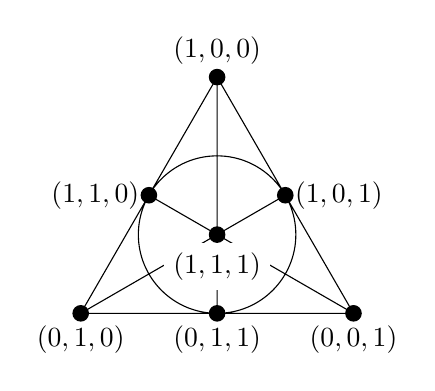
\begin{tikzpicture}
  \draw (30:1)  -- (210:2)
        (150:1) -- (330:2)
        (270:1) -- (90:2)
        (90:2)  -- (210:2) -- (330:2) -- cycle
        (0:0)   circle (1);
  \fill (0:0)   circle(3pt) node[below,fill=white,yshift=-3pt,xshift=0pt]{$(1,1,1)$}
        (30:1)  circle(3pt) node[right]{$(1,0,1)$}
        (90:2)  circle(3pt) node[above,yshift=1pt,xshift=0pt]{$(1,0,0)$}
        (150:1) circle(3pt) node[left]{$(1,1,0)$}
        (210:2) circle(3pt) node[below,yshift=-1pt]{$(0,1,0)$}
        (270:1) circle(3pt) node[below,yshift=-1pt]{$(0,1,1)$}
        (330:2) circle(3pt) node[below,yshift=-1pt]{$(0,0,1)$};
\end{tikzpicture}
\end{center}
\caption{A depiction of the Fano plane $F_7$. Each straight line is an edge, and the circle is an edge; each edge contains exactly 3 vertices, since $F_7$ is a 3-graph.} \label{fig:Fano}
\end{marginfigure}


Recall that $c: V(H)\to [k]$ is a $k$-coloring of a hypergraph $H$ if no edge of $H$ is monochromatic, and $\chi(H)$ is the minimum $k$ such that $H$ admits a $k$-coloring. We have the following lemma.
\begin{lemma} \label{lem:chiF7}
\[	
\chi(F_7) = 3.
\]
\end{lemma}
\begin{proof}	
In a random $3$-coloring, the probability that an edge is monochromatic is $\frac{1}{9}$, so the expected number of monochromatic edges is $\frac{7}{9}<1$. So there exists a 3-coloring with no monochromatic edges. So $\chi(H) \leq 3$.

Suppose there exists a 2-coloring of $F_7$. Then by pigeonhole, at least four vertices have to recieve the same color; say $w,x,y,z$, say with color 1. Since $\{x,y,x+y\}$ is an edge: $x+y+x+y = 2x+2y = 0$, we must have $x+y$ be color 2; similarly with $y+z$ and $x+z$. But then $\{x+y,y+z,x+z\}$ is a monochromatic edge, of color 2.
\end{proof}

\begin{marginfigure}
\begin{center}
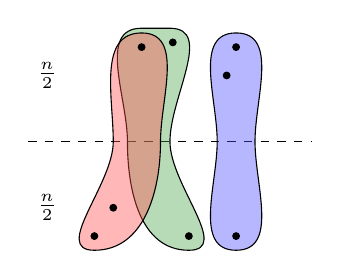
\begin{tikzpicture}[color=black,scale=1.2]
\def\radius{1}

\node at (-.5, 1.7) {\small $\tfrac{n}{2}$};

\node at (-.5, .3)  {\small $\tfrac{n}{2}$};

\draw[dashed] (-.7,1) -- (2.3,1);
\begin{scope}
\node (a3) at (0,0){};
\node (a4) at (1,0){};
% \node (a5) at (2,0) {};
\node (a2) at (.5,1) {};
\node (a1) at (.5,2) {};
\begin{scope}[fill opacity=.4]


  \filldraw[fill=green!70] ($(a1) + (.3,0.2)$) 
        to[out=0,in=90] ($(a2)+(.3,0)$)
        to[out=270,in=0] ($(a4) + (0,-.15)$)
        % to[out=180,in=0] ($(a4) + (0,-.1)$)
        to[out=180,in=270] ($(a2)+(-0.15,0)$)
        to[out=90,in=180] ($(a1)+(0,.2)$) -- cycle;


  \filldraw[fill=red!70] ($(a1) + (0,0.15)$) 
        to[out=0,in=90] ($(a2)+(.2,0)$)
        to[out=270,in=0] ($(a3) + (0,-.15)$)
        % to[out=180,in=0] ($(a3) + (0,-.1)$)
        to[out=180,in=270] ($(a2)+(-0.3,0)$)
        to[out=90,in=180] ($(a1)+(0,.15)$);


\end{scope}

\filldraw (a3) circle (\radius pt) node{};
\filldraw ($(a3) +(.2,.3)$) circle (\radius pt) node{};

\filldraw (a4) circle (\radius pt) node{};
\filldraw (a1) circle (\radius pt) node{};
\filldraw ($(a1) + (.33,.05)$) circle (\radius pt) node{};

\end{scope}

\begin{scope}[xshift=1.5cm,yshift=2cm,rotate=180]
\node (a3) at (0,0){};
\node (a4) at (1,0){};
% \node (a5) at (2,0) {};
\node (a2) at (0,1) {};
\node (a1) at (0,2) {};
\begin{scope}[fill opacity=.4]

  \filldraw[fill=blue!70] ($(a1) + (0,0.15)$) 
        to[out=0,in=90] ($(a2)+(.2,0)$)
        to[out=270,in=0] ($(a3) + (0,-.15)$)
        % to[out=180,in=0] ($(a3) + (0,-.1)$)
        to[out=180,in=270] ($(a2)+(-0.2,0)$)
        to[out=90,in=180] ($(a1)+(0,.15)$);


\end{scope}

\filldraw (a3) circle (\radius pt) node{};
% \filldraw (a4) circle (\radius pt) node{};
\filldraw (a1) circle (\radius pt) node{};
\filldraw ($(a3) +(.1,.3)$) circle (\radius pt) node{};

\end{scope}

\end{tikzpicture}
\end{center}
\caption{A $3$-graph on $n$ verticies formed by partitioning the verticies in two approximately equal parts, and choosing edges as all triples with at least one vertex in each part. For clarity, not all the edges are drawn here.} \label{fig:3graph_one_from_each}
\end{marginfigure}
If we partition $n$ verticies into two approximately equal halves, we may define a $3$-graph by declaring all triples with at least one member in each half to be edges; see \cref{fig:3graph_one_from_each} for an illustration.
There are $\frac{3}{4}{n\choose 3} + O(n^2)$ edges in this graph. If this graph had a Fano plane subgraph, then we could 2-color the Fano plane, which is impossible by \cref{lem:chiF7}. Thus, the graph of \cref{fig:3graph_one_from_each} must not have an $F_7$ subgraph, so $\pi(F_7)\geq \frac{3}{4}$.
%  We see that this is impossible by first considering the triangle (verticies $\{a,w,c\}$ in \cref{fig:fano_labelled}); if those three verticies were monochromatic red, then the circle $\{b,y,z\}$ must be monochromatic blue (or else one of the sides of the triangle would be monochromatic red). In either case, if the Fano plane were 2-colorable, then one vertex of the triangle must be a different color than the other two. Let's say $a$ is red, while $w$ and $c$ are blue. Then $z$ must be red or else $\{c,z,w\}$ would be monochromatic blue. Since $\{a,x,z\}$ is an edge, $x$ must be blue. For $\{b,x,w\}$ and $\{c,x,y\}$ to not be monochromatic blue  edges, both $b$ and $y$ must be red. This yields $\{b,y,z\}$ as a monochromatic red edge.
% \begin{marginfigure}
% \begin{center}
% \begin{tikzpicture}
% \def\radius{2}
% \def\shift{1}
%   \draw (30:1)  -- (210:2)
%         (150:1) -- (330:2)
%         (270:1) -- (90:2)
%         (90:2)  -- (210:2) -- (330:2) -- cycle
%         (0:0)   circle (1);
%   \fill[blue] (0:0)   circle(\radius pt) node[left,yshift=0pt,xshift=-3pt](x){$x$};
%   \fill      (30:1)  circle(\radius pt) node[right,xshift=\shift pt](y){$y$};
%   \fill[red]     (90:2)  circle(\radius pt) node[above,yshift=\shift pt,xshift=0pt](a){$a$};
%   \fill      (150:1) circle(\radius pt) node[left, xshift=-\shift pt](b){$b$};
%   \fill[blue]      (210:2) circle(\radius pt) node[left,yshift=0pt, xshift=-\shift pt](c){$c$};
%   \fill[red]      (270:1) circle(\radius pt) node[below,yshift=-\shift pt](z){$z$};
%   \fill[blue]      (330:2) circle(\radius pt) node[below,yshift=-\shift pt](w){$w$};
%   %   \draw[blue] (0:0) -- (30:1) node[midway,above]{$L_c$}
%   %         (270:1) -- (330:2) ;
%   %   \draw[red!30]
%   %       (270:1) -- (0:0) node[midway,left]{$L_a$}
%   %       (30:1) -- (330:2);
%   %   % \draw[green]
%   %     % (270:1) -- ;
%   % \draw[green] (270:1) arc (270:270+120:1);
%   % \draw[green] (0:0) -- (330:2) node[near start]{$L_b$} ;
% \end{tikzpicture}
% \end{center}
% \caption{A depiction of the proof to show that the Fano plane is impossible to 2-color. } \label{fig:fano_labelled}
% \end{marginfigure}

% \missingfigure{Partition vertices into two parts of size $\sim \frac{n}{2}$, and take all edges which have $\geq 1$ vertex in each part. This hypergraph contains $\sim \frac{3}{4}{n\choose 3}$ edges, so $\pi(F_7) \geq \frac{3}{4}$.}
\begin{theorem}[\cite{DeCaenFuredi}] 
\[	
\pi(F_7) = \frac{3}{4}.
\]
\end{theorem}
\begin{proof}	
Suppose not: $\pi(F_7) = \frac{3}{4}+ 2 \epsilon$ for some $\epsilon>0$. By \cref{lem:subgraph_with_min_vertex_degree},  for every $n_0$ there exists a $3$-graph $G$ on $n\geq n_0$ vertices with no $F_7$ subgraph such that every vertex of $G$ belongs to $\geq ( \frac{3}{4} + \epsilon) {n\choose 2}$ edges. Moreover, we may assume that $G$ contains $K_4^{(3)}$: four vertices such that every triple forms an edge\sidenote{If not, every set of four verticies yields at most three edges, which implies $G$ has at most $\frac{3}{4}{n\choose 2}$ edges in total, contradicting our assumption.}.
% \unsure{why can we do this?}
 We'll take these vertices to be $a,b,c,d$.
% \marginnote{Lecture 14: Wednesday, February 24, 2016.}
\lect{2}{24}

For $x\in V(G)$, let $L_x = \{ \{y,z\}: \{x,y,z\} \in \edges (G) \}$. This is called the \defn{link graph} of $x$ in $G$.
For $x_1,x_2,\dotsc,x_k$ we will consider $L_{x_1} \cup L_{x_2} \cup \dotsm \cup L_{x_k}$ (abusing notation) as a \defn{multigraph}, meaning that we count multiplicity.

\begin{claim}
If $\{a,b,c\}\in \edges (G)$, then $L_a \cup L_b\cup L_c$ induces at most 15 edges (counting multiplicity) on any four vertices. \marginnote{A single link graph can induce ${4 \choose 2} = 6$ edges on four vertices, so our naive bound is 18. Our claim is that this additional structure of being link graphs of $G$ lets us do slightly better.}
\end{claim}



\begin{marginfigure}
\begin{center}
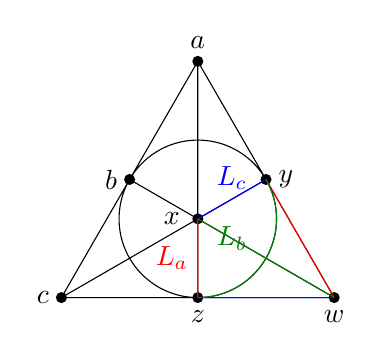
\begin{tikzpicture}
\def\radius{2}
\def\shift{1}
  \draw (30:1)  -- (210:2)
        (150:1) -- (330:2)
        (270:1) -- (90:2)
        (90:2)  -- (210:2) -- (330:2) -- cycle
        (0:0)   circle (1);
  \fill (0:0)   circle(\radius pt) node[left,yshift=0pt,xshift=-3pt](x){$x$}
        (30:1)  circle(\radius pt) node[right,xshift=\shift pt](y){$y$}
        (90:2)  circle(\radius pt) node[above,yshift=\shift pt,xshift=0pt](a){$a$}
        (150:1) circle(\radius pt) node[left, xshift=-\shift pt](b){$b$}
        (210:2) circle(\radius pt) node[left,yshift=0pt, xshift=-\shift pt](c){$c$}
        (270:1) circle(\radius pt) node[below,yshift=-\shift pt](z){$z$}
        (330:2) circle(\radius pt) node[below,yshift=-\shift pt](w){$w$};
    \draw[blue] (0:0) -- (30:1) node[midway,above]{$L_c$}
    			(270:1) -- (330:2) ;
   	\draw[red]
   			(270:1) -- (0:0) node[midway,left]{$L_a$}
   			(30:1) -- (330:2);
   	% \draw[green]
   		% (270:1) -- ;
	\draw[green] (270:1) arc (270:270+120:1);
	\draw[green] (0:0) -- (330:2) node[near start]{$L_b$} ;
\end{tikzpicture}
\end{center}
\caption{%The Fano plane, labelled, with the complete 2-graph on $\{x,y,z,w\}$ colored. 
Given an edge $\{a,b,c\}$, we consider any four vertices $x,y,z,w \in L_a\cup L_b\cup L_c$, and on these seven vertices, we construct the Fano plane. Since $G$ contains no $F_7$ subgraph, the edges drawn here must not all appear in the link graphs.\label{fig:fano_link_graphs}}
\end{marginfigure}
\begin{subproof}[Proof of claim.]	

Let $x,y,z,w$ be vertices in $V(G) \setminus \{a,b,c\}$. As $G$ contains no $F_7$, there does not exist a partition of the edge set of the complete 2-graph on $\{x,y,z,w\}$ into three subsets $M_1,M_2,$ and $M_3$ of size two such that  $|M_1\cap L_a|=2, |M_2\cap L_b|=2,$ and $|M_3\cap L_c|=2$; see \cref{fig:fano_link_graphs}. 

Suppose $L_a\cup L_b\cup L_c$ has $\geq 16$ edges on $\{x,y,z,w\}$, i.e., these link graphs missed at most 2 out of the maximum possible number of edges (which is $3*{4\choose 2} = 18$, recalling that we count edges in the link graphs with multiplicity).
Let 
\begin{align*}	
M_1 &=\{ \{x,y\}, \{z,w\} \}, &
M_2 &= \{ \{ x,w \}, \{ y,z \} \}, &
M_3 &=\{ \{x,z\}, \{ y,w \} \}
\end{align*}
as shown in \cref{fig:complete_graph_in_links_fano}. 
Up to changing the labels, there are two cases.
\begin{marginfigure}
\begin{center}
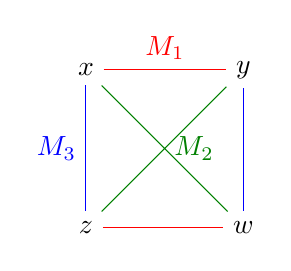
\begin{tikzpicture}[scale=2]
\node (x) at (0,1) {$x$};
\node (y) at (1,1) {$y$};

\node (z) at (0,0) {$z$};

\node (w) at (1,0) {$w$};

\draw[green] (x) -- (w) node[midway,right]{$M_2$}
			(y) -- (z);

\draw[blue]
			(x) -- (z) node[midway,left]{$M_3$}
			(y) -- (w);

\draw[red]
			(x) -- (y) node[midway,above]{$M_1$}
			(z) -- (w);

\end{tikzpicture}	
\end{center}
\caption{A choice of partition $M_1,M_2,M_3$ of edges of the complete graph on  $\{x,y,z,w\}$, chosen to correspond to \cref{fig:fano_link_graphs}.  \label{fig:complete_graph_in_links_fano}}
\end{marginfigure}
\begin{enumerate}[{Case }1:]
	\item  Both missing edges belong to $M_1$. That is, either for some $x\in \{a,bc\}$, we have $|L_x\cap M_1| = 0$ or for some $x,y\in \{a,b,c\}$ distinct, we have $|L_x\cap M_1| = 1$ and $|L_y\cap M_1| = 1$.

  In any case, $M_1$ fully intersects with one of the $L_x$; say, $L_a$ (that is, $|L_a\cap M_1|= 2$). Then since those were the only two missing edges, we have $|L_b\cap M_2| = |L_c\cap M_3|=2$. 
   % Then wlog $M_1\subset L_a$, $M_2\subset L_b$, $M_3\subset L_c$. ($M_1$ belongs to one link graph).
	\item One missing edges belongs to $M_1$ and one $M_2$. That is, $|M_1\cap L_x| = 1$ and $|M_2\cap L_y| = 1$, for some $x,y\in\{a,b,c\}$. Since those were the only missing edges, $M_1$ fully intersects with two link graphs, and $M_2$ with two. So we may choose them to be different, putting, say, $|M_1\cap L_a|=2$, $|M_2\cap L_b|=2$, and $|M_3\cap L_c|=2$.\qedhere
  % As before, for some $x$, we still have $|M_1\cap L_x| = 2$
  % Then wlog $M_1\subset L_a$ (belongs to 2 link graphs), $M_2\subset L_b$ ($M_2$ belongs to 1 link graph not $L_a$), and $M_3\subset L_c$.
\end{enumerate}
\end{subproof}

\begin{claim}
If $a,b,c,d$ are the vertices of $K_4^{(3)}$, then $L_a\cup L_b\cup L_c\cup L_d$ induces at most 20 edges counted with multiplicies in $V(G)\setminus \{a,b,c,d\}$.
\end{claim}
\begin{subproof}	
Apply previous claim to all 4 edges $\{a,b,c\}$, $\{a,b,d\}$, $\{a,c,d\}$, $\{b,c,d\}$. In total, the resulting multigraph will have at most 60 edges but each $L_i$ (for $i\in \{a,b,c,d\}$) is counted 3 times.
\end{subproof}

Then,
\[
|L_a \cup L_b\cup L_c \cup L_d| \geq (3 + \epsilon) {n \choose 2}
\]
If we restrict to $L_a\cup L_b\cup L_c\cup L_d$ to $V(G)\setminus \{a,b,c,d\}$, we still have at least 
\begin{equation} \label{eq:numedges} \tag{$\star$f}
(3+ \epsilon){n\choose 2} - 12n
\end{equation}
 edges, where we've overcounted edges in $L_a\cup L_b\cup L_c\cup L_d$ using one of $\{a,b,c,d\}$.

\marginnote{Note in the following, we are considering $2$-graphs.}
We may think of a multigraph with vertex set $V$ as a function $w: V^{(2)} \to \Z_+$.
Let $m(n,k,r)$ be the maximum number of edges (the sum of weights $\sum_{e\in V^{(2)}} w(e)$) in a multigraph on $n$ vertices such that any $k$ vertices induce $\leq r$ edges.
We will show that 
\begin{equation} \label{eq:max_multigraph_edges} \tag{$\star$}
m(n,4,20) \leq 3 {n\choose 2} + n -2
\end{equation}
for $n\geq 4$. This will finish the proof, as it contradicts (\ref{eq:numedges}) for large $n$.
We will assume 
\begin{equation} \label{eq:assumption_for_max_multigraph} \tag{$\star\star$}
m(n,3,10) \leq 3 {n\choose 2} + n-2.
\end{equation}
The proof of this is left as an exercise.
Let us prove (\ref{eq:max_multigraph_edges}) by induction.
Base case: 
\[
m(4,4,20) \leq 3\cdot 6 + 4-2 = 20.
\]
Induction step: Using (\ref{eq:assumption_for_max_multigraph}), we assume $\{a,b,c\} \subset V$  induces $k\geq 11$ edges. Let $w(x)= \sum_{e\ni x} w(e)$ for $x\in \{a,b,c\}$.
Then
\begin{align*}	
w(a) +w(b) + w(c) &= \underbrace{2k}_{\substack{\text{weight of edges} \\ \text{ with two of $\{a,b,c\}$}}} + \sum_{z\in V\setminus \{a,b,c\}} ( w(za) + w(zb) + w(zc))
\end{align*}
 Since every four verticies span at most 20 edges, for each $z\in V\setminus \{a,b,c\}$ we have $w(za) +w(zb) + w(zc)  \leq 20-k$.  Then 
\begin{align*}
w(a) + w(b)+ w(c) &\leq
2k + (n-3) (20-k) \\
&= 20(n-3) - k(n-5)\\
&\leq 20 (n-3) - 11(n-5) = 9n-5
\end{align*}
WLOG, $w(a) \leq 3n-2$ by pigeonhole.
By the induction hypothesis, $V\setminus \{a\}$ induces total weight at most
\[
3 {n-1 \choose 2} + (n-1)-2.
\]
So the total number of edges is at most
\[
 3 {n-1 \choose 2} + (n-1)-2 + (3n-2) \leq 3 {n\choose 2} + n-2. \qedhere
\]
\end{proof}
% section hypergraph_turan_problems (end)

\begin{fullwidth}
\printbibliography[segment=\therefsegment,heading=subbibliography]
\end{fullwidth}
\clearpage

%\input{chapters/midterm}

\clearpage
\newrefsegment
%!TEX root = ../CombinatoricsNotes.tex

\section{Ramsey Theory}
\marginnote{``Every sufficiently large system contains a regular subsystem.''}

Consider a two coloring $C: [n]^{(2)}\to \{R,B\}$ where $R$ stands for red and $B$, blue.
A \defn{regular subsystem} is a subset $X\subset [n]$ such that $c$ restricted to $X^{(2)}$ takes only one value\marginnote{That is, the coloring restricted to $X$ is monochromatic.}.
The \defn{Ramsey number} $R(k,\ell)$ is the minimum number $n$ such that for every $c: [n]^{(2)} \to \{R,B\}$, there exists $X\subset[n]$ such that either
\begin{itemize}
	\item $c$ restricted to $X^{(2)}$ is identically $R$ and $|X|=k$, or
	\item \ditto{$c$ restricted to $X^{(2)}$ is identically} $B$ and $|X| = \ell$.
\end{itemize}
\begin{remark}
The existence of Ramsey numbers was first shown by Frank Ramsey (\cite{ramsey1930problem}), as a lemma to proving the decidability of a class of formulas in first order logic. Here, we will present a short proof by \erdos  and Szekeres.
\end{remark}
\begin{theorem}[\cite{erdosszekeres1935combinatorial}]
~\begin{itemize}
	\item $R(k,\ell)$ exists for all $k$ and $\ell$,
	\item $R(k,\ell) \leq R(k-1,\ell) + R(k,\ell-1)$ for $k,\ell\geq 2$, and
	\item $R(1,\ell) = R(k,1) = 1$. 
\end{itemize}
\end{theorem}
\begin{proof}	
Let $n = R(k-1,\ell) + R(k,\ell-1)$. Choose $v\in [n]$; then, either
\begin{enumerate}[(1)]
  \item  $v$ is joined to $\geq R(k-1,\ell)$ verticies by red edges. In this case choosing an appropriate $X$ among the red neighbors of $v$ gives the result, or
  \item $v$ is joined to $(n-1) - (R(k-1,\ell)-1) = R(k,\ell-1)$ verticies by blue edges. This case is analogous.
\end{enumerate}
This yields $R(k,\ell) \leq R(k-1,\ell) + R(k,\ell-1)$. The third point follows from the definition, and the first inductively from this inequality, using the third point as the base case.
\end{proof}
In fact, we may obtain a bound on the $R(k,\ell)$ in this way.
\begin{corollary}
\[
R(k,\ell)\leq {k+\ell -2 \choose k-1}
\]
for all $k,\ell \geq 1$.
\end{corollary}
\begin{proof}  
If $k=1$ or $\ell=1$ then $R(k,\ell)=1$. Otherwise, by induction
\begin{align*}  
R(k,\ell) &\leq R(k-1,\ell) + R(k,\ell)-1 \\
&\leq {k+\ell -3 \choose k-2} + {k+\ell -3 \choose k-1} = {k+\ell-2 \choose k-1}.\qedhere
\end{align*}
\end{proof}
\begin{remark}
In particular, $R(k,k) \leq {2k-2\choose k-1} \sim \frac{4^k}{\sqrt{k}}$. We in fact have $R(3,3) = 6$, $R(4,4)=18$, and $43\leq R(5,5) \leq 49$. 
\end{remark}

\begin{theorem}[\cite{erdos1947someremarks}]
$R(k,k)\geq 2^{k/2}$ for $k\geq 2$.
\end{theorem}
\begin{proof}  
Let $n = \floor{2^{k/2}}$ and let $c:[n]^{(2)}\to \{R,B\}$ be chosen unifomrly randomly. That is, the color of every edge in $[n]^{(2)}$ is chosen to be $R$ with probability $1/2$ or $B$ with probability $1/2$, independently of the other edges. Let $Z$ be equal to the number of sets $X\subset[n]$, $|X|=k$, such that $c$ restricted to $X^{(2)}$ is monochromatic. It is enough to show $\E[Z] < 1$. \marginnote{Since then there must be exist some coloring with $Z<1$, i.e., $Z=0$.}
For fixed $X$ as above,
\[
\Pr[c \text{ restricted to }X\text{ is monochromatic}] = \frac{1}{2^{{k\choose 2}-1}}.
\]
Then
\begin{align*}  
\E[Z] &= {n\choose k} 2^{1 - {k\choose 2}}\leq \frac{n^k}{k!}2^{1 - \frac{k(k-1)}{2}}\\
&\leq \frac{2^{k^2/2}\cdot 2^{1 + (k/2) - k^2/2}}{k!} = \frac{2^{1+k/2}}{k!}<1
\end{align*}
for $k\geq 3$. One may show $R(2,2) = 2$, yielding the case $k=2$.
\end{proof}
The state of the art bounds are
\marginnote{Lower: \cite{SPENCER1975}, upper: \cite{conlon2009new}.}
% \begin{theorem*}[]
\[
(1 + O(1)) \frac{\sqrt{2}k}{e}2^{k/2}\leq R(k,k) \leq k^{- \frac{c\log k}{\log \log k}}4^k.
\]
% \end{theorem*}


\newthought{Next, if $n$ is sufficiently large} with respect to $k$ and $c:[n]\to \{R,B\}$, then $[n]$ contains a monochromatic \defn{arithmetic progression} of length $k$, that is a set\marginnote{Note that here we are discussing colorings of $[n]$, not $[n]^{(2)}$; that is, vertex colorings, not edge colorings.}
\[
\{ a, a+d ,\dotsc, a+(k-1)d\}
\]
for some $d>0$. We may write this as $a + [0,k-1]d$, where $[0,k-1] = \{ j\in \Z: 0\leq j\leq k-1\}$ and the addition and multiplication is elementwise. The \defn{Van der Waerden number} $W(k,r)$ is the minimum $n$ such that if $[n]$ is colored in $r$ colors one can always find a monochromatic arithmetic progression of length $k$.

% \missing{Missed class: Monday, March 7}
\begin{theorem}[\cite{VdWaerden1927}]
$W(k,r)$ exists for all $r,k$. \label{thm:VdW}
\end{theorem}
The proof will follow from \cref{lem:Wkmr}.
\begin{example}
\begin{itemize}
	\item $W(2,r) = r+1$ \marginnote{by pigeonhole}
	\item $W(k,1) = k$,
	\item What about $W(3,2)$? Well, \rdot\rdot\bdot\bdot\rdot\rdot\bdot\bdot \,shows $W(3,2) > 8$.  On the other hand, assuming the 5th slot is red, wlog, we reduce to two cases:
	\begin{align*}	
	\vartextvisiblespace \rdotm \vartextvisiblespace \bdotm \rdotm \bdotm \vartextvisiblespace \rdotm \vartextvisiblespace\\
	\rdotm\rdotm\bdotm\bdotm\rdotm\rdotm\bdotm\bdotm\vartextvisiblespace
	\end{align*}

	Let's outline the general argument; this will give a bound $W(3,2) \leq 5 \times 65 = 325$. Color $[325]$ and divide it into $65$ intervals of length~5.
\newcommand{\vdwdots}{\rdot\bdot\bdot\rdot\rdot}
\newcommand{\firstpic}{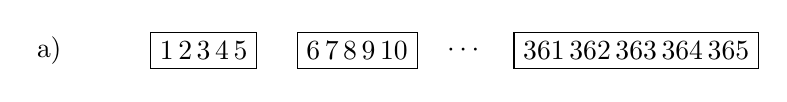
\begin{tikzpicture}[node distance = .5cm]
	\node[draw] (n1) at (0,0) {1\,2\,3\,4\,5};
	\node[left = 1cm of n1]{a)};
	\node[draw,right= of n1] (n2)  {6\,7\,8\,9\,10};

	\node[right= .25cm of n2] (n7)  {$\dotsm$};
	\node[draw,right= .25cm of n7] (n10)  {361\,362\,363\,364\,365};
	\end{tikzpicture}}
	\newcommand{\secondpic}{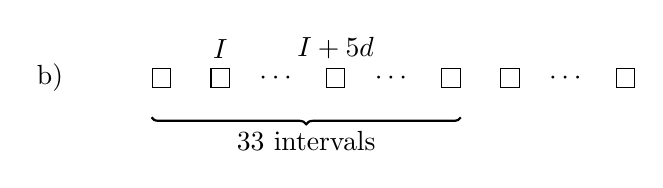
\begin{tikzpicture}[node distance = .5cm]
	\node[draw] (n1) at (0,0) {\phantom{\vdwdots}};
	\node[left = 1cm of n1]{b)};

	\node[draw,label=above:$I$,right=of n1] (n2) {\vdwdots};
	\node[right= .25cm of n2] (n3)  {$\dotsm$};
	\node[draw,right=.25cm of n3,label=above:$I+5d$] (n4)  {\vdwdots};
	\node[right= .25cm of n4] (n5)  {$\dotsm$};
	\node[draw,right= .25cm of n5] (n6)  {\phantom{\vdwdots}};
	\node[draw,right= of n6] (n6p5)  {\phantom{\vdwdots}};
	\node[right= .25cm of n6p5] (n7)  {$\dotsm$};
	% \node[draw,right=.25cm of n7,label=above:$I+10d$] (n8)  {\rdot\bdot\bdot\rdot\rdot};
	% \node[right= .25cm of n8] (n9)  {$\dotsm$};
	\node[draw,right= .25cm of n7] (n10)  {\phantom{\vdwdots}};
\draw [
    thick,
    decoration={
        brace,
        mirror,
        raise=0.5cm
    },
    decorate] (n1.west) --  (n6.east) node [pos=0.5,anchor=north,yshift=-0.55cm] {$33$ intervals};
	\end{tikzpicture}}

\newcommand{\thirdpic}{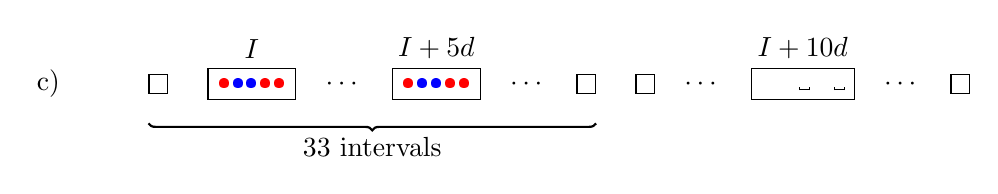
\begin{tikzpicture}[node distance = .5cm]
	\node[draw] (n1) at (0,0) {\phantom{\vdwdots}};
	\node[left = 1cm of n1]{c)};
	\node[draw,label=above:$I$,right=of n1] (n2) {\rdot\bdot\bdot\rdot\rdot};
	\node[right= .25cm of n2] (n3)  {$\dotsm$};
	\node[draw,right=.25cm of n3,label=above:$I+5d$] (n4)  {\rdot\bdot\bdot\rdot\rdot};
	\node[right= .25cm of n4] (n5)  {$\dotsm$};
	\node[draw,right= .25cm of n5] (n6)  {\phantom{\vdwdots}};
	\node[draw,right=  of n6] (n6p5)  {\phantom{\vdwdots}};
	\node[right= .25cm of n6p5] (n7)  {$\dotsm$};
	\node[draw,right=.25cm of n7,label=above:$I+10d$] (n8)  {\phantom{\rdot\bdot} \textvisiblespace \phantom{\rdot} \textvisiblespace};
	\node[right= .25cm of n8] (n9)  {$\dotsm$};
	\node[draw,right= .25cm of n9] (n10)  {\phantom{\vdwdots}};
\draw [
    thick,
    decoration={
        brace,
        mirror,
        raise=0.5cm
    },
    decorate] (n1.west) --  (n6.east) node [pos=0.5,anchor=north,yshift=-0.55cm] {$33$ intervals};
	\end{tikzpicture}}
\begin{figure*}[ht]
\begin{center}


\begin{tabular}{l}
\firstpic\\[1.25em]
 \secondpic \\[1.25em]
\thirdpic
\end{tabular}

\end{center}

\caption{a) We subdivide $[325]$ into 65 intervals of length $5$. b) By the pigeonhole principle, two of the first $2^5+1=33$ intervals have same coloring. If $I$ is the first interval; then for some $d>0$, the second is $I+5d$. c) To complete the proof, we consider $I+10d$, as described in the text.} \label{fig:VdW_ex_33int}
\end{figure*}
	Consider the first $2^5+1=33$ of them. Two of them will be colored exactly the same by pigeonhole; say interval $I$ and interval $I+5d$. If $I = [a,a+5]$, then $\{a,a+d',a+2d'\}$ is an arithmetic progression for $d'\in \{1,2\}$. Now, if either of these progressions are monochromatic, then we are done. Otherwise, say we have $\{{\color{blue} a },{\color{blue} a+d' },{ \color{red} a+2d' } \}$\sidenote{If $a$ and $a+d'$ are different colors, then choose the other $d'$.}, for $d'\in \{1,2\}$. Now, we consider the interval $I+10d$. If $a+2d' + 10d$ is red, then $\{a+2d',a+2d'+5d, a+2d' + 10d\}$ is monochromatic red. Otherwise $a,a+d'+5d, a+2d' + 10d$ is monochromatic blue. 

\end{itemize}
\end{example}

A \defn{polychromatic $m$-tuple}  of arithmetic progression of length $k$ is a set $A = \{a + [0,k]d_1\} \cup \{ a + [0,k]d_2\} \cup \dotsm \cup \{a + [0,k]d_m\}$ such that $a+ [1,k]d_i$ is monochromatic for all $i$, and all of these $m$ progressions are of different colors (see \cref{fig:polymk} for an example).
\lect{3}{9}

\begin{marginfigure}
\[
 \stackrel{\text{\textvisiblespace}}{0}\,\stackrel{\rdotm}{1}\,\stackrel{\rdotm}{2}\,\stackrel{\gdotm}{3}\,\stackrel{\bdotm}{4}\,\stackrel{\text{\textvisiblespace}}{5} \,\stackrel{\gdotm}{6}\,\stackrel{\text{\textvisiblespace}}{7}\,\stackrel{\bdotm}{8}
\]
\caption{With the coloring shown, $\{ 0 + [0,2]\} \cup \{0 + [0,2]\cdot 3\} \cup \{0 + [0,2]\cdot 4\}$ is a  polychromatic $3$-tuple of length $2$.}\label{fig:polymk}
\end{marginfigure}


\begin{lemma} \label{lem:Wkmr}
If $W(k-1;r)$ exists for every $r$ then for every $m$ there exists $W(k,m,r) = n$ such that in any $r$-coloring of $[n]$ there exists a monochromatic a.p. of length $k$ or a polychromatic $m$-tuple of a.p. of length $k-1$.
\end{lemma}
\begin{remark}
With this result,  \cref{thm:VdW} follows by induction on $k$, using that $W(k;r) \leq W(k,r+1,r)$, since there cannot exist a polychromatic $r+1$-tuple when there are only $r$ colors.
\end{remark}
\begin{proof}[Proof by induction on $m$.] Base case: $m=1$. Then in a set of size $W(k-1,r)$ we may find a monochrome $(k-1)$-a.p., say $a+d[1,k]$; then for a polychromatic 1-tuple of a..p of length $k$, we simply need to add the point $a$. We may ensure this by taking a second copy of $W(k-1,r)$ to the left, yielding the bound $ W(k,1,r) \leq 2W(k-1,r)$ (see \cref{fig:vdwclaim_basecase} for an illustration).
\begin{marginfigure}
\begin{center}
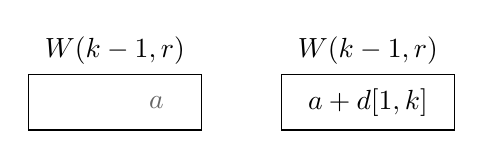
\begin{tikzpicture}
 \node[draw,label={above:$W(k-1,r)$},minimum width = 2.2cm, minimum height = .7cm] (n1) at (0,0) {$a+d[1,k]$};
\node[draw,left= of n1,minimum width = 2.2cm,minimum height = .7cm,text opacity = .6, label={above:$W(k-1,r)$}] {\quad\qquad$a$};
 \end{tikzpicture} 
\end{center}
\caption{Depiction  showing $ W(k,1,r) \leq 2W(k-1,r)$ by finding a monochrome  $(k-1)$-a.p. $a  + d[1,k]$ in a set of size $W(k-1,r)$ and adding in the point $a$, which may be to the left of the original set of size $W(k-1,r)$.} \label{fig:vdwclaim_basecase}
\end{marginfigure}

To show the induction step, we will first prove the following result.
\begin{claim}
 If $A+d,A+2d,\dotsc, A+(k-1)d$ are \emph{identically colored}\sidenote{For each $x\in A+d$, we have that $x,x+d,\dotsc,x+(k-2)d$ all have the same color.} polychromatic $m$-tuples of a.p. of length $(k-1)$ then $A\cup (A+d)\cup\dotsm \cup (A+ (k-1)d)$ contains a polychromatic $(m+1)$-tuple of a.p. of length $k-1$, or a monochromatic a.p. of length $k$.
\end{claim}
\begin{subproof}
~\medskip

\begin{figure*}
\begin{center}
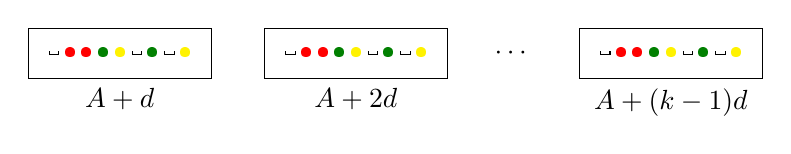
\begin{tikzpicture}[color=black]
\def\xdiff{1}
\def\xlength{2}

\node (B1) at (0,0){};

\node (B2) at (\xdiff+\xlength,0){};

\node (B3) at (3*\xdiff+2*\xlength,0){};


\foreach \n in {1,2,3}
{
\node (B\n s0) at (B\n){\textvisiblespace};
\node (B\n s1) at (B\n s0)[right]{\rdot};
\node (B\n s2) at (B\n s1)[right]{\rdot};
\node (B\n s3) at (B\n s2)[right]{\gdot};
\node (B\n s4) at (B\n s3)[right]{\ydot};
\node (B\n s5) at (B\n s4)[right]{\textvisiblespace};
\node (B\n s6) at (B\n s5)[right]{\gdot};
\node (B\n s7) at (B\n s6)[right]{\textvisiblespace};
\node (B\n s8) at (B\n s7)[right]{\ydot};
}

\node[draw,fit = (B1s0) (B1s8),label=below:$A+d$]{};
\node[draw,fit = (B2s0) (B2s8),label=below:$A+2d$]{};
\node[draw,fit = (B3s0) (B3s8),label=below:$A+(k-1)d$]{};


\node (dots) at ($(B2s0)!0.5!(B3s8)$) {$\dotsm$};

\end{tikzpicture}

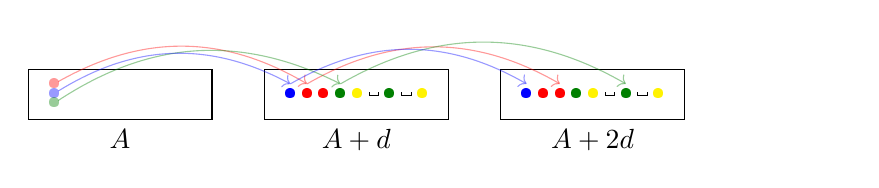
\begin{tikzpicture}[color=black]
\def\xdiff{1}
\def\xlength{2}

\node (B0) at (-\xdiff-\xlength,0){};

\node (B1) at (0,0){};

\node (B2) at (\xdiff+\xlength,0){};

\node (B3) at (3*\xdiff+2*\xlength,0){};


\foreach \n in {0,1,2}
{
\ifthenelse{\n=0}
{
\def\opt{\phantom}
\node[opacity=.4] (B\n s0) at ($(B\n) + (0,0)$){\bdot};
\node[opacity=.4] (B\n s0r) at ($(B\n) + (0,.12)$){\rdot};
\node[opacity=.4] (B\n s0g) at ($(B\n) + (0,-.12)$){\gdot};
}
{
\def\opt{}
\node (B\n s0) at (B\n){\bdot};
}



\node (B\n s1) at (B\n s0)[right]{\opt\rdot};
\node (B\n s2) at (B\n s1)[right]{\opt\rdot};
\node (B\n s3) at (B\n s2)[right]{\opt\gdot};
\node (B\n s4) at (B\n s3)[right]{\opt\ydot};
\node (B\n s5) at (B\n s4)[right]{\opt\textvisiblespace};
\node (B\n s6) at (B\n s5)[right]{\opt\gdot};
\node (B\n s7) at (B\n s6)[right]{\opt\textvisiblespace};
\node (B\n s8) at (B\n s7)[right]{\opt\ydot};
}

\node[draw,fit = (B1s0) (B1s8),label=below:$A+d$]{};
\node[draw,fit = (B2s0) (B2s8),label=below:$A+2d$]{};
\node[draw,fit = (B0s0) (B0s8),label=below:$A$]{};
% \tikzset{ar/.style={bend left,->,yshift=-3pt,shorten >=2pt,shorten <=2pt}}
\tikzset{ar/.style={bend left,->,yshift=-2pt,opacity=.4}}


\newcommand\ar[4]{
	\draw[#1]
	($(#2.east) + (-.16,.11) $) edge[ar] ($(#3.north)$);	
	\draw[#1]
	($(#3.north)$) edge[ar] ($(#4.north)$);
}
\ar{red}{B0s0r}{B1s1}{B2s2}

\ar{green}{B0s0g}{B1s3}{B2s6}
\ar{blue}{B0s0}{B1s0}{B2s0}


% \draw[blue]
% 	(B0s0) edge[ar] (B1s0) 
% 	edge [ar] (B2s0);
% \draw[red]
	% (B0s0) edge[ar] 
	% (B1s1) edge [ar] ($(B2s2.north)$);	
% \draw[green]
% 	(B0s0) edge[ar] ($(B1s3.north)$)
% 	edge [ar] (B2s6);	


% \node (dots) at ($(B1s8)-(B1s0)$) {$\dotsm$};

\end{tikzpicture}
\end{center}

\caption{Upper: an example of identically colored $m$-tuples of arithmetic progressions (with $k=3$). Below: Possible constructions of a monotone $k$-a.p.} \label{fig:VdWlemmafig}
\end{figure*}

% \missingfigure{Box labelled $A+d$ with blank, red, red, green, yellow, blank, green, blank, yellow. Box $A+2d$ with same dots. Horizontal dots. Box $A+(k-1)d$ with same dots. Now add a blue dot to the beginning of each, and draw a box to the far left labelled $A$. The far left element is $a$. Then $a$ to 0-slot in $A+d$ to 0-slot of $A+2d$ is a.p. Another is $a$ to $1$-slot in $A+d$ to $2$-slot in $A+2d$. Antoher is $a$ to first green of $A+d$ to second green of $A+2d$. And $a$ to first yellow in $A+d$ to second yellow in $A+2d$.(In this example, $k-1=2$)}
% Let $c$ be denote the coloring. Each $A+\ell d$ for $\ell\in[k-1]$ has the same set of colors:
% \[
%  c(A+d):= \{c(x): x\in A+d\} = c(A+2d) = \dotsm = c(A+(k-1)d).
%  \] 
%  We write $A+d=\bigcup_{i=1}^m \{a+d+d_i[0,k-1]\}$ where each $a+d+d_i[0,k-1]$ is monochromatic and differently colored from $a+d+d_j[0,k-1]$ for $i\neq j$.  In this language, the identical coloring assumption is that $\{ a+\ell d + s d_i: \ell \in [k-1] \}$ is monochromatic for each $s \in [0,k-1]$.

%  Now, we look at each element of $A$ in turn. Consider the first element, $a$. If $c(a) \in c(A+d)$, then let $c(a) = c(a+d+sd_i)$ for $s\in [k-1]$. Then, by our identical coloring assumption,
%  \[
%  \{ a, a+d+sd_i,a+2d+sd_i, \dotsc,a+(k-1)d  +sd_i \}
%  \]
%  is a monochromatic a.p. of length $k$.  Let us consider an arbitrary element of $A$, $a+ xd_j$ for $x \in [0,k-1]$ and $i\in[m]$. If $c(a+xd_j) = c(a + d + sd_i)$ for $i\in[m]$ and $s\in[0,k-1]$, then

 Write $A+d=\bigcup_{i=1}^m \{a+d+d_i[0,k-1]\}$ where each $a+d+d_i[0,k-1]$ is monochromatic and differently colored from $a+d+d_j[0,k-1]$ for $i\neq j$. In this language, the identical coloring assumption is that $\{ a+\ell d + s d_i: \ell \in [k-1] \}$ is monochromatic for each $s \in [0,k-1]$.
 %Then the a.p. $a+sd+d_i[1,k-1]$ is monochromatic for every $i=1,\dotsc,m$ and $s=1,\dotsc,k-1$ (the color does not depend on $s$).
In particular, 
\[
 P':=\{a+d,a+2d,\dotsc,a+(k-1)d\}
 \] is a monochromatic $(k-1)$-a.p.  If it  is the same as color as $a+d+d_i$ for some $i$, then 
 \[
 \{ a+d, a+d+d_i,a+d+2d_i,\dotsc,a+d+(k-1)d_i\}
 \]
is a monochromatic $k$-a.p.
Otherwise,
%
% Indeed, if $A\cup(A+d)\cup \dotsm \cup (A+(k-1)d)$ contains no monochromatic $k$-term a.p. then 
% \[
%  P':=\{a+d,a+2d,\dotsc,a+(k-1)d\}
%  \] all are of the same color and different from the color of other a.p. in $A+sd$.
% 
consider
\[
 P_i':=\{a+d+d_i,a+2d+2d_i,\dotsc,a+(k-1)d+(k-1)d_i\}
 \] which is an a.p. of the same color as 
 \[
 \{a+d+d_i,a+d+2d_i,\dotsc,a+d+(k-1)d_i\}.
 \]
and thus a different color from $P'$. Then $P'\cup P_1'\cup\dotsc\cup P_m'\cup\{a\}$ is a polychromatic $(m+1)$-tuple. \qedhere \marginnote{This is the meat of the proof.}
\end{subproof}


Now let $M = W(k,m,r)$ and $N = W(k-1,r^M)$. We will show that $W(k,m+1;r)\leq 2MN$. 

% \missingfigure{Partition into two intervals of length $MN$, and the second into $N$ intervals of length $M$ (by underbraces and overbraces). I can think of the second half as a coloring of $N$ into $r^M$ colors (we encode the coloring of an interval of length $M$ as a single color of the $r^M$ colors). }
\begin{figure*}
\begin{center}
\begin{tikzpicture}[node distance = .5cm, every node/.style={minimum height=.7cm}]
	\node[draw,left= of n1] (nL)  {\qquad\qquad\qquad\qquad\qquad\qquad\qquad\quad};

	\draw [
    thick,
    decoration={
        brace,
        mirror,
        raise=0.5cm
    },
    decorate] (nL.west) --  (nL.east) node [pos=0.5,anchor=north,yshift=-0.55cm] {$MN$};
	

	\node[draw,label=below:] (n1) at (0,0) {\qquad\qquad\quad};
	\node[draw,right= of n1] (n2)  {\qquad\qquad\quad};

	\node[right= .25cm of n2] (n3)  {$\dotsm$};
	\node[draw,right= .25cm of n3] (n4)  {\qquad\qquad\quad};


		\draw [
    thick,
    decoration={
        brace,
        mirror,
        raise=0.5cm
    },
    decorate] (n1.west) --  (n4.east) node [pos=0.5,anchor=north,yshift=-0.55cm] {$N$ intervals};


    \draw [
    thick,
    decoration={
        brace,
        raise=0.5cm
    },
    decorate] (n1.west) --  (n1.east) node [pos=0.5,anchor=north,yshift=1.2cm] {$M$};

 \draw [
    thick,
    decoration={
        brace,
        raise=0.5cm
    },
    decorate] (n2.west) --  (n2.east) node [pos=0.5,anchor=north,yshift=1.2cm] {$M$};
     \draw [
    thick,
    decoration={
        brace,
        raise=0.5cm
    },
    decorate] (n4.west) --  (n4.east) node [pos=0.5,anchor=north,yshift=1.2cm] {$M$};
	\end{tikzpicture}
\end{center}
\caption{We think of coloring each interval  of size $M$ on the right side into $r$ colors as assigning the entire interval one of $r^M$ colors.}\label{fig:vdw_ind_step}
\end{figure*}
We divide $2MN$ into an interval of size $MN$ followed by $N$ intervals of size $M$, as shown in \cref{fig:vdw_ind_step}.
By choice of $N$, there are intervals $(k-1)$ intervals on the right side of the form $I,I+d,I+2d,\dotsc,I+(k-2)d$  which are identically colored.

By the choice of $M$, we may assume $I$ contains a polychromatic $m$-tuple of a.p. of length $(k-1)$ which we will call $A+d$. The first interval of size $MN$ serves to include $A$. The induction step is finished by the claim.
\end{proof}
The proof yields very poor bounds for $W(k;r)$. The current best bounds are
\marginnote{LHS: folklore with a randomized construction. RHS: \cite{Gowers2001}.}
\[
(1 + o(1)) \frac{r^k}{erk} < W(k;r) \leq 2^{2^{r^{2^{2^{k+9}}}}}.
\]
It's conjectured that the upper bound can be improved substantially:
\begin{conjecture*}
 $W(k;2) \leq 2^{k^2}$.
\end{conjecture*}
Let us proceed to the Hales-Jewett theorem.
 It may be informally stated as the following: in a $\overbrace{t\times t\dotsm \times t}^{d \text{ dimensional}}$ game of tic-tac-toe with $r$ players, a draw is impossible as long as $d$ is large enough compared to $r$ and $t$.
Let $A$ be a finite alphabet of size $t$, typically $[0,t-1]$. 
Then $A^d$ is the set of ordered $d$-tuples of elements of $A$, or words of length $d$ in the alphabet $A$. 

In tic-tac-toe, $A = \{0,1,2\}$, and $d=2$ (see \cref{fig:tic-tac-toe}). We think of each player having a color; a coloring of $\{0,1,2\}^2$ by two colors then corresponds to the moves made by both the players. A draw is impossible if  in any coloring of $\{0,1,2\}^2$, there is a monochromatic ``3-in-a-row'', i.e.,  row, column, or diagonal.
\begin{marginfigure}
\begin{center}
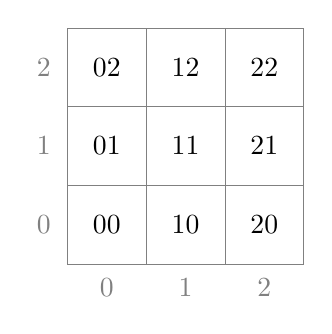
\begin{tikzpicture}

\def\xshift{3.5}

\tikzset{side/.style={gray, thin}}

\draw[step=1cm,gray,very thin] (0,0) grid (3,3);

\foreach \x in {0,1,2}
{
\node[side] at ($ (-.3,.5) +(0,\x) $)  {\x};
\node[side] at ($ (.5,-.3) +(\x,0) $)  {\x};
	\foreach \y in {0,1,2}
	{
	\node at ($ (\x,\y) + (0.5,0.5) $) {\x\y};
	}
}
\end{tikzpicture}
\end{center}
\caption{A depiction of  words in tic-tac-toe: elements of $\{0,1,2\}^2$.} \label{fig:tic-tac-toe}
\end{marginfigure}
% \missingfigure{3x3 grid, labelled 0,1,2 going up and going right from bottom left. Write ordered pairs in the boxes. Possible roots: $\tau_1=0\star$, $\tau_2=\star\star$. The line associated with $\tau_1$ is the first column. The linea ssociated with $\tau_2$ is the diagonal. The middle row is a combinatorial line associated with $\star 1$. The diagonal from top left to bottom right is not a combinatorial line.}
\begin{figure*}[ht]

\begin{center}
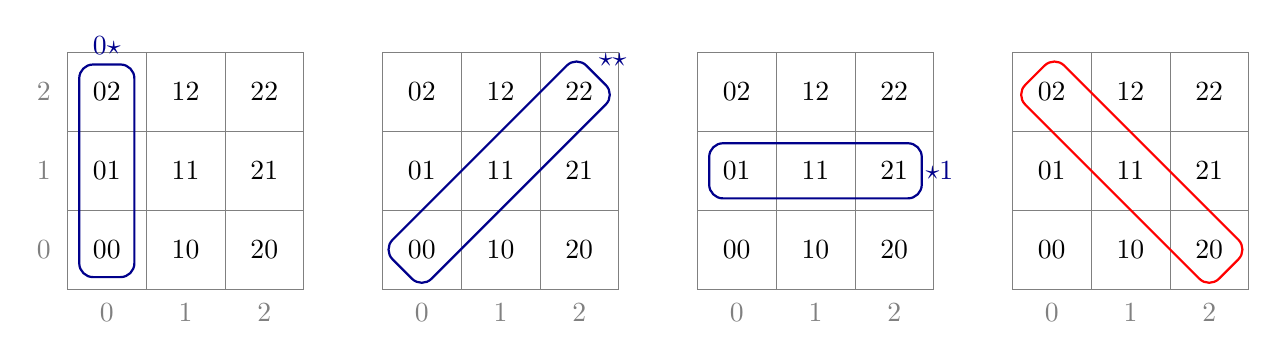
\begin{tikzpicture}
\tikzset{side/.style={gray, thin}}
\tikzset{combline/.style={draw, DarkBlue, rounded corners=5pt, thick}}

\def\xshift{4};

\begin{scope}
\draw[step=1cm,gray,very thin] (0,0) grid (3,3);

\foreach \x in {0,1,2}
{
\node[side] at ($ (-.3,.5) +(0,\x) $)  {\x};
\node[side] at ($ (.5,-.3) +(\x,0) $)  {\x};
	\foreach \y in {0,1,2}
	{
	\node at ($ (\x,\y) + (0.5,0.5) $) {\x\y};
	}
}
\def\off{.15};

\draw[combline,label=above:$0\stars$] (\off,\off) rectangle (1-\off,3-\off);

\node[above,DarkBlue] at (.5,3-\off){$0\star$};
\end{scope}


\begin{scope}[shift={(\xshift,0)}]

\draw[step=1cm,gray,very thin] (0,0) grid (3,3);

\foreach \x in {0,1,2}
{
% \node[side] at ($ (-.3,.5) +(0,\x) $)  {\x};
\node[side] at ($ (.5,-.3) +(\x,0) $)  {\x};
	\foreach \y in {0,1,2}
	{
	\node (\x\y) at ($ (\x,\y) + (0.5,0.5) $) {\x\y};
	}
}
\def\off{.15};
%rotate around={30:(-1,0.5)}

\draw[combline,label=above:$0\stars$,rotate around={-45:(.5,0.5)}] (\off,\off) rectangle ($ (1-\off,1.41*3-4*\off) $);

\node[above,DarkBlue] at (3-.5*\off,3-2*\off){$\star\star$};
\end{scope}


\begin{scope}[shift={(2*\xshift,0)}]
\draw[step=1cm,gray,very thin] (0,0) grid (3,3);

\foreach \x in {0,1,2}
{
% \node[side] at ($ (-.3,.5) +(0,\x) $)  {\x};
\node[side] at ($ (.5,-.3) +(\x,0) $)  {\x};
	\foreach \y in {0,1,2}
	{
	\node (\x\y) at ($ (\x,\y) + (0.5,0.5) $) {\x\y};
	}
}
\def\off{.15};
%rotate around={30:(-1,0.5)}



\draw[combline,label=above:$0\stars$] (\off,1+\off) rectangle ($ (3-\off,2-\off) $);

\node[right,DarkBlue] at (3-1.5*\off,1.5){$\star 1$};
\end{scope}


\begin{scope}[shift={(3*\xshift,0)}]

\draw[step=1cm,gray,very thin] (0,0) grid (3,3);

\foreach \x in {0,1,2}
{
% \node[side] at ($ (-.3,.5) +(0,\x) $)  {\x};
\node[side] at ($ (.5,-.3) +(\x,0) $)  {\x};
	\foreach \y in {0,1,2}
	{
	\node (\x\y) at ($ (\x,\y) + (0.5,0.5) $) {\x\y};
	}
}
\def\off{.15};
%rotate around={30:(-1,0.5)}

\begin{scope}[xshift=2cm]
\draw[combline,Red,rotate around={45:(.5,0.5)}] (\off,\off) rectangle ($ (1-\off,1.41*3-4*\off) $);
\end{scope}

% \node[above,DarkBlue] at (3-.5*\off,3-2*\off){$\star\star$};
\end{scope}



\end{tikzpicture}


\end{center}
\caption{Three examples of combinatorial lines in $\{0,1,2\}^2$, followed by a nonexample.  From left to right, combinatorial lines corresponding to roots $\tau_1 = 0\star$, $\tau_2 = \star\star$, and $\tau_3 = \star 1$, respectively, followed by the set $\{02,11,20\}$ in red which is not a combinatorial line. So in tic-tac-toe, not every ``3-in-a-row'' is a combinatorial line, but every combinatorial line is a ``3-in-a-row'', which is enough to show that draws are impossible if we can always find a monochromatic combinatorial line.  } \label{fig:comb_lines_in_tic_tac_toe}
\end{figure*}



Moving back to the general development, a \defn{root} $\tau$ is a word of length $d$ in the alphabet $A\cup \{\star\}$, where $\star$ is a symbol not in $A$, which contains at least one $\star$.
For a root $\tau$ and $a\in A$, the word $\tau(a)$ is obtained by substituting $a$ instead of $\star$ everywhere in $\tau$. A \defn{combinatorial line} in $A^d$ is a set $L_\tau:=\{ \tau(a): a\in A\}$ where $\tau$ is a root of length $d$. See \cref{fig:comb_lines_in_tic_tac_toe} for examples and nonexamples of combinatorial lines in tic-tac-toe. With these definitions, we may formulate the Hales-Jewett theorem as follows. 
\begin{theorem}[\cite{halesJewett1963regularity}] \label{thm:HJ}
For every $r$ and $t$, there exists $d= \HJ(t,r)$ such that if $A$ is an alphabet with $|A|=t$ and $A^d$ is colored in $r$ colors, then there exists a monochromatic combinatorial line. 
\end{theorem}
\begin{remark}
The same is true for every $d' \geq d$.
\end{remark}
Before proving the Hales-Jewett theorem, we'll discuss an application. 
Let $V\subset \Z^d$ be a finite collection of vectors. $U$ is called a homothetic copy of $V=\{v_1,v_2,\dotsc,v_t\}$ if $U = u +\lambda V = \{ u + \lambda v_1,u+\lambda v_2,\dotsc, u+\lambda v_t\}$ for some $u\in \Z^d$ and $\lambda\in \Z$. Homothetic copies are a generalization of arithmetic progressions: for $d=1$ and $V = \{0,1,\dotsc,k-1\}$, a homothetic copy of $V$ is exactly an arithmetic progression of length $k$. See  \cref{fig:homothetic_ex} for a two dimensional example.
\begin{marginfigure}[2cm]
\begin{center}
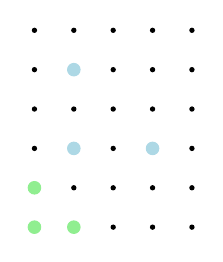
\begin{tikzpicture}[scale=.5]
% \draw[step=1cm,gray,very thin] (0,0) grid (4,5);
\def\rad{1.5pt}

\foreach \x in {0,1,...,4}
{
	\foreach \y in {0,1,...,5}
	{
		\filldraw[black] (\x,\y) circle (\rad);
	}
}
\filldraw[LightGreen] (0,0) circle (3*\rad);
\filldraw[LightGreen] (0,1) circle (3*\rad);
\filldraw[LightGreen] (1,0) circle (3*\rad);

\def\lam{2};
\def\ux{1};
\def\uy{2};


\filldraw[LightBlue] ($ (\ux ,\uy) + \lam*(0,0)  $)  circle (3*\rad);
\filldraw[LightBlue] ($ (\ux ,\uy)  + \lam*(0,1)  $) circle (3*\rad);
\filldraw[LightBlue] ($ (\ux ,\uy)  + \lam*(1,0)  $) circle (3*\rad);

\end{tikzpicture}
\end{center}
\caption{An example of homothetic copies in $\Z^2$: the green dots are $V = \{(0,0),(0,1),(1,0)\}$, and the blue dots are $U= u +\lambda V$ for $u = (1,2)$ and $\lambda=2$.} \label{fig:homothetic_ex}
\end{marginfigure}
\begin{theorem}[Gallai (late 1930s), \cite{Wit_paper}]\marginnote{According to \textcite[page 22]{Ramsey_Yesterday_today_tomorrow}, this theorem was communicated from Gallai to Rado in the late 1930s, and was published in 1943 (\cite{Rado_note}). The theorem was independently proven by Wit in 1952.}
Let $\Z^d$ be colored in $r$ colors and let $V\subset \Z^d$ be finite. Then there exists a monochromatic homothetic copy of $V$.
\end{theorem}
\begin{remark}
In fact, one can replace $\Z^d$ by $[n]^d$ where $n$ depends on $V$ and $r$, yielding an analog of van der Waerden's theorem.
\end{remark}
\begin{proof}	
The proof will be based on the  HJ theorem.

We will take an appropriately large hypercube and project it into $\Z^d$ such that a combinatorial line in the hypercube projects to a homothetic copy of $V$.
Let $V = \{v_1,\dotsc,v_t\} =: A$. Let $n$ be such that every $r$-coloring of $A^n$ contains a monochromatic combinatorial line.

Define $f: A^n\to \Z^d$ by $f((a_1,a_2,\dotsc,a_n)) = \sum_{i=1}^n a_i$ where $a_i \in V$. If $\chi$ is the coloring of $\Z^d$ into $r$-colors, then we can define $\chi': A^n \to [r]$ by $\chi'(a) = \chi(f(a))$. By the choice of $n$, there exists a root $\tau$ such that $\tau(v_1)$, $\tau(v_2)$, \ldots, $\tau(v_t)$ all receive the same color. Then $\{f(\tau(v_1)), f(\tau(v_2)), \ldots,f( \tau(v_t))\}$ is a homothetic copy of $V$, as follows. If $\tau = a_1a_2\dotsm a_n$ then set  $u := \sum_{i: a_i\neq \star} a_i$, and $\lambda$  the number of $\star$'s in $\tau$. Then $f(\tau(v_i)) = u+ \lambda v_i$.

\flavor{This is the end, but let me make you believe that this is the end.}

For example, consider $V=\{v_1,v_2,v_3\}$ and $\tau= v_1 v_2 \star v_1 \star$. Then we're claiming $\{f(\tau(v_1)),f(\tau(v_2)),f(\tau(v_3))\}$ is a homothetic copy of $V$. E.g.,
\[
f(\tau(v_1)) =  v_1 + v_2 + v_1  +v_1 + v_1 =4v_1  + v_2 = \underbrace{v_1+v_2 +v_1}_{u} + \underbrace{2}_\lambda v_1. \qedhere
\]
\end{proof}
\flavor{Paraphrase: Proofs by logicians are the hardest; I can follow it but I don't understand why things are happening.}

\lect{3}{14}
% \marginnote{Lecture X: Monday, March 14, 2016.}

\begin{proof}[Proof of \cref{thm:HJ}]
Let $n = \HJ(t,r)$. We will prove its existence by induction on $t$ for fixed $r$.
First, $\HJ(1,r)=1$, since combinatorial lines of length 1 are certainly monochromatic.

Now, the induction step. Assume $n = \HJ(t-1,r)$. Let $n\ll N_1 \ll N_2 \ll \dotsm \ll N_n$. Specifically, $N_1 = r^{t^n}$ and $N_i = r^{t^n + \sum_{j=1}^{i-1} N_j}$ for $i\geq 2$, and $N = \sum_{i=1}^n N_i$. We will show that $\HJ(r,t)\leq N$, i.e. if $\chi: A^N \to [r]$, then $\chi$ contains a monochromatic combinatorial line.

% \missingfigure{ long versions of \textvisiblespace labelled $N_1$ to $N_n$ }
\begin{figure}
\begin{center}
\vspace{\baselineskip}
\begin{tikzpicture}[node distance = 1cm]
\def\ydif{.1};
\def \nmax {3};
\coordinate (1A) at (0,0);

\coordinate (1Au) at ($ (1A) + \ydif*(0,1) $);
\draw (1A) -- (1Au);

\coordinate[right= of 1A] (1B);
\coordinate (1Bu) at ($ (1B) + \ydif*(0,1) $);
\draw (1B) -- (1Bu);


\draw (1A) -- (1B) node[midway, label={below:$N_1$}]{};

\foreach \n in {2,3,...,\nmax}
{
	\pgfmathparse{int(\n -1 )};

	\coordinate[right= of \pgfmathresult B] (\n A);

	\coordinate (\n Au) at ($ (\n A) + \ydif*(0,1) $);
	\draw (\n A) -- (\n Au);

	\coordinate[right= of \n A] (\n B);
	\coordinate (\n Bu) at ($ (\n B) + \ydif*(0,1) $);
	\draw (\n B) -- (\n Bu);


	\draw (\n A) -- (\n B) node[midway, label={below:$N_\n$}]{};
}

% \pgfmathparse{};
\pgfmathsetmacro{\nplusone}{int(\nmax +1)}

\node[right = of \nmax B] (\nplusone B) {$\dotsm$};

\pgfmathparse{int(\nmax +2)};

\pgfmathsetmacro{\nplustwo}{int(\nmax +2)}

\coordinate[right= of \nplusone B] (\nplustwo A);

\coordinate (\nplustwo Au) at ($ (\nplustwo A) + \ydif*(0,1) $);
\draw (\nplustwo A) -- (\nplustwo Au);

\coordinate[right= of \nplustwo A] (\nplustwo B);
\coordinate (\nplustwo Bu) at ($ (\nplustwo B) + \ydif*(0,1) $);
\draw (\nplustwo B) -- (\nplustwo Bu);


\draw (\nplustwo A) -- (\nplustwo B) node[midway, label={below:$N_n$}]{};

\end{tikzpicture}
% \vspace{-.5\baselineskip}
\end{center}
\caption{A depiction of $N_1,\dotsc,N_n$. We aim to show $\HJ(t,r) = N:= \sum_{i=1}^n N_i$.} \label{fig:HJ1}
\end{figure}
We will say $a,b\in A^n$ are \emph{neighbors} if they differ in only one position and one of them has symbol $0$ in this position and the other has the symbol $1$; that is, if $a = a_1a_2\dotsm a_{i-1} 0 a_{i+1} \dotsm a_n$, and $b =a_1a_2\dotsm a_{i-1} 1 a_{i+1} \dotsm a_n$ for some $1\leq i \leq n$.

Let $\tau$ be a root of length $N$ such that $\tau = \tau_1\dotsm \tau_n$ and $\tau_i$ is a root of length $N_i$. For $a \in A^n$, $a = a_1\dotsm a_n$, define
\[
\tau(a) = \tau_1(a_1)\tau_2(a_2)\dotsm \tau_n(a_n).
\]
For example, suppose we have a root $\tau=\overbrace{\star}^{\tau_1} \overbrace{2\star}^{\tau_2} \overbrace{\star 3\star}^{\tau_3}$. Then $\tau(012) = 021232$.
Given $\tau = \tau_1\tau_2\dotsm \tau_n$ as above, define $\chi_\tau: A^n \to [r]$ by $\chi_\tau(a) = \chi(\tau(a))$.
Now, we're not guaranteed that we have monochromatic combinatorial lines in $A^n$, but we will try to compress to $A^{n-1}$ where we do have such lines.
\begin{claim}
There exist roots $\tau_1,\tau_2,\dotsc,\tau_n$ such that $\tau_i$ has length $N_i$, and, if $\tau=\tau_1\dotsm \tau_n$, then
\[
\chi_\tau(a) = \chi_\tau(b)
\]
for any pair of neighbors $a$ and $b$ in $A^n$.
\end{claim}
We accept this claim for now to finish the proof. Define $\chi'_\tau$ as the restriction $\chi_\tau': (A\setminus \{0\})^n \to [r]$ of $\chi_\tau$. Then $\chi_\tau'$ contains a monochromatic combinatorial line. That is, there exists $\nu = \nu_1\nu_2\dotsm \nu_n$ with $\nu_i\in (A\setminus\{0\})\cup \{\star\}$ such that $\nu(1),\nu(2),\dotsc,\nu(t-1)$ all have the same color. We wish to show that the line corresponding to $\tau(\nu)$ is monochromatic in $\chi: A^N\to[r]$, where we write $\tau(\nu) := \tau_1(\nu_1)\dotsm \tau_n(\nu_n)$ with $\tau_i(\star)=\tau_i$.
\marginnote{If $\nu = (12\star)$, then $\tau(\nu) = 122\star 3\star$, using our example $\tau$ from earlier.}
That is, we want $\tau(\nu(0))$, $\tau(\nu(1))$,\ldots, $\tau(\nu(t-1))$ to receive the same color in $\chi$. So we want $\chi_\tau(\nu(a))$ to be the same for $a=0,1,\dotsc,t-1$.

But $\chi_\tau(\nu(1)) = \dotsm = \chi_\tau(\nu(t-1))$ by the choice of $\nu$. So it remains to show that $\chi_\tau(\nu(0))=\chi_\tau(\nu(1))$.  While $\nu(0)$ and $\nu(1)$ may differ in several positions, in each position one has 1 and the other has 0, so we may change them one at a time using that $\chi_\tau$ acts the same on neighbors, until we see they have the same coloring.

Thus, it remains to prove the claim. We will construct the roots $\tau_1,\dotsc,\tau_n$ in reverse order.
Suppose $\tau_{i+1},\dotsc,\tau_n$ are constructed.\marginnote{The case $\tau_n$ is similar to the generic step we consider here.}
% \missingfigure{Intervals $N_1, N_2$, \ldots $N_{i-1}$, $N_i$ with $W_k$, $N_{i+1}$ with $\tau_{i+1}$, \ldots, $N_n$ with $\tau_n$. Overbrace from $N_1$ to $N_{i-1}$ by $M$.}
For $0\leq k\leq N_i$, let
\[
W_k = \underbrace{0\dotsm 0}_k \underbrace{1\dotsm 1}_{N_i-k}\in A^{N_i}
\]
Let $M = \sum_{j=1}^{i-1}N_i$. Define a coloring  $\chi_k : A^{M+ n-i} \to [r]$ as
\[
\chi_k(x_1 \dotsm x_M y_{i+1}\dotsm y_{n}) =  \chi(x_1\dotsm x_M W_k \tau_{i+1}(y_{i+1})\dotsm \tau_n(y_n)).
\]
See \cref{fig:vdwWk} for a depiction of this definition.
\begin{figure*}[ht]
\begin{center}
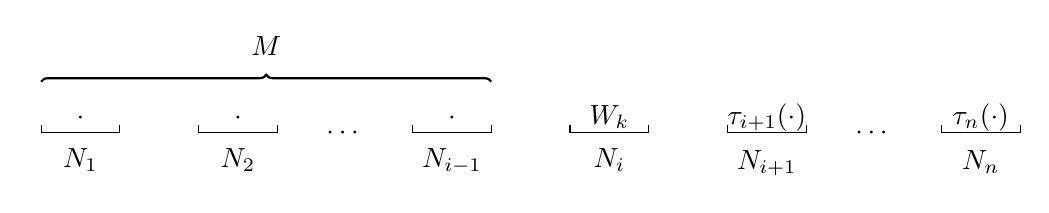
\begin{tikzpicture}[node distance = 1cm]
\def\ydif{.1};
\def\dotsdist{.5};

\setcounter{numint}{0};
\coordinate (0B) at (0,0);
\stepcounter{numint}

\newcommand{\vdwinterval}[3][1]{
	\def\n{\thenumint};
	\pgfmathparse{int(\thenumint - 1)};

	\coordinate[ node distance = #1 cm, right= of \pgfmathresult B] (\n A);

	\coordinate (\n Au) at ($ (\n A) + \ydif*(0,1) $);
	\draw (\n A) -- (\n Au);

	\coordinate[right= of \n A] (\n B);
	\coordinate (\n Bu) at ($ (\n B) + \ydif*(0,1) $);
	\draw (\n B) -- (\n Bu);


	\draw (\n A) -- (\n B) node[midway, label={below:$N_{#2}$},yshift=.2cm]{#3};

	\stepcounter{numint}
}
\vdwinterval{1}{\phantom{$W_k$}$\cdot$\phantom{$W_k$}}
\vdwinterval{2}{\phantom{$W_k$}$\cdot$\phantom{$W_k$}}

\newcommand{\vdwdots}{
	\def\n{\thenumint};
	\pgfmathparse{int(\thenumint - 1)};

	\node[node distance = \dotsdist cm, right = of \pgfmathresult B] (\n B) {$\dotsm$};
	\stepcounter{numint}
}
\vdwdots
\vdwinterval[\dotsdist]{i-1}{\phantom{$W_k$}$\cdot$\phantom{$W_k$}}
\vdwinterval{i}{$W_k$}
\vdwinterval{i+1}{$\tau_{i+1}(\cdot)$}
\vdwdots
\vdwinterval[\dotsdist]{n}{$\tau_n(\cdot)$}

\draw [
    thick,
    decoration={
        brace,
        raise=0.65cm
    },
    decorate] (1A.west) --  (4B.east) node [pos=0.5,anchor=north,yshift=1.35cm] {$M$};


\end{tikzpicture}
\end{center}
\caption{An illustration of how $\chi_k$ acts on words in $A^{M+n-i}$. First, we write such a word as $x_1\dotsm x_m y_{i+1}\dotsm y_n$ where $x_j \in A^{N_j}$ (for $j\in [i-1]$) and $y_j \in A$ (for $j=i+1,\dotsc,n$). Then, $\chi_k$ acts on such a word by creating a word of size $A^N$ as follows, which it plugs into $\chi$.  First, $x_1,\dotsc,x_m$ are not modified (visualized by empty slots of the appropriate size in the figure). Then  the word $W_k \in A^{N_i}$ is concatenated, followed by $\tau_{j}(y_j) \in A^{N_j}$ for $j= i+1,\dotsc,n$.} \label{fig:vdwWk}
\end{figure*}
% Suppose $\tau_{i+1}$
Now, $N_i > t^{M+n - i}$, so there exist $k,\ell$ such that $\chi_k = \chi_\ell$, by the pigeonhole principle. WLOG $k< \ell$. Let $\tau_i = \underbrace{0\dotsm0}_k \underbrace{\star\dotsm\star}_{\ell-k} \underbrace{1\dotsm 1}_{N_i - \ell}$. Then $\tau_i(0) = W_\ell$ and $\tau_i(1) = W_k$.

Now, let's show that the resulting $\tau = \tau_1\dotsm \tau_n$ satisfies the claim. Suppose $a = a_1a_2\dotsm a_{i-1} 0 a_{i+1} \dotsm a_n$, and $b =a_1a_2\dotsm a_{i-1} 1 a_{i+1} \dotsm a_n$. Then 
\begin{align*}	
\chi_\tau(a) &= \chi(\tau_1(a_1)\tau_2(a_2)\dotsm \tau_{i-1}(a_{i-1})W_\ell \tau_{i+1}(a_{i+1})\dotsm \tau_n(a_n)) \\
&= \chi_\ell (\tau_1(a_1)\tau_2(a_2)\dotsm \tau_{i-1}(a_{i-1})W_\ell a_{i+1}\dotsm a_n)\\
&= \chi_k (\tau_1(a_1)\tau_2(a_2)\dotsm \tau_{i-1}(a_{i-1}) a_{i+1}\dotsm a_n)\\
&= \chi_\tau(b).\qedhere
\end{align*}
\end{proof}
%should 7.8
\begin{theorem}[Density Hales-Jewett theorem, \cite{DensityHJ}] \label{thm:HJ_density}
For every $\epsilon>0$ and each $t$, there exist $n$ such that if $|A| = t$ and $Z \subset A^n$ with $|Z| \geq \epsilon t^n$ then $Z$ contains a combinatorial line.
\end{theorem}
\begin{remark}
This theorem implies \cref{thm:HJ}. If we consider an $r$-coloring as a partition $Z_1,\dotsc,Z_r$ of $A^n$, then we have some $i$ such that $|Z_i| \geq \frac{1}{r}t^n$ by the pigeonhole principle. Then \cref{thm:HJ_density} with $\epsilon= \frac{1}{r}$ implies that $Z_i$ contains  combinatorial line, proving \cref{thm:HJ}.
\end{remark}

%thm. 7.9
\begin{theorem}[\cite{szemeredi1975sets}]
$\forall \, \epsilon>0$ and $\forall\, k$, $\exists N > 0$ such that if $A\subset [N]$ with $|A| \geq \epsilon N$, then $A$ contains an arithmetic progression of length $k$.
\end{theorem}


%thm. 7.10
\begin{theorem}[\cite{green2008primes}]
For every $k$, the set of primes contain arithmetic progressions of length $k$. \marginnote{Since the density of primes goes to zero, the density theorem above does not help.}
\end{theorem}


If we wanted to formulate a density version of Ramsey's theorem, how it would it go? For every $t$ and $\epsilon>0$, there exists $N$ such that if $G$ is a graph on $N$ verticies  and $|G|\geq \epsilon {N\choose 2}$, then $G$ contains $K_t$.
But this is equivalent to $\pi(K_t) = 0$, which is false for $t\geq 3$.

\newthought{Let us} move on. Consider a finite sequence $A=(a_1,\dotsc,a_n)$. Then we say $(a_{i_1},a_{i_2},\dotsc,a_{i_k})$ is an \defn{increasing subsequence}[subsequence!increasing] of $A$ if $i_1 < i_2 < \dotsb< i_k$ and $a_{i_1}\leq a_{i_2} \leq \dotsm \leq a_{i_k}$. Likewise, $(a_{i_1},a_{i_2},\dotsc,a_{i_k})$ is a \defn{decreasing subsequence}[subsequence!decreasing] of $A$ if $i_1 < i_2 < \dotsb< i_k$ and $a_{i_1}\geq a_{i_2} \geq \dotsm \geq a_{i_k}$. 

\begin{problem}
For all $k$, does there exist a number $f(k)$ such that every sequence of length at least $f(k)$ contains an increasing or decreasing subsequence of length $k$?
\end{problem}

Indeed, such an $f(k)$ exists: $f(k) \leq R(k,k)$. Given a sequence $(a_n)_{n=1}^{R(k,k)}$, we can create a coloring on $[R(k,k)]$ as follows: given an edge $\{i,j\}\in [R(k,k)]^{(2)}$  with $i<j$, we color $\{i,j\}$ red if $a_i\leq  a_j$, and blue otherwise. Then by the definition of $R(k,k)$, we are guaranteed  a monochromatic complete graph on $k$ verticies. This yields an increasing subsequence if the monochromatic $K_k$ is red, and decreasing if the $K_k$ is blue. This yields an exponential bound on $f(k)$. But we can do better.
\begin{theorem}[\cite{erdosszekeres1935combinatorial}]
For all $k,\ell\geq 2$ any sequence of length at least $(k-1)(\ell-1)+1$ contains an increasing subsequence of length $k$ or a decreasing subsequence of length $\ell$.
\end{theorem}
\begin{remark}
In the case $k=\ell$, this is a quadratic bound on $f(k)$.
\end{remark}
\begin{proof}[Proof by induction on $k+\ell$]	
If $k=2$, say, then any sequence of length $\ell$ is decreasing or not.
For the induction step, let $n = (k-1)(\ell-1) + 1$,  $A=(a_1,\dotsc,a_n)$ be a sequence, and $Z$ be the set of last elements of increasing subsequences of length $k-1$ in $A$. Then, $Z = (a_{i_1},a_{i_2},\dotsc,a_{i_z})$ with $i_1< \dotsm < i_z$, where $z = |Z|$. For contradiction, assume $A$ violates the claim.

Then $A\setminus Z$ contains no increasing subsequences of length $k-1$ and no decreasing subsequences of length $\ell$. So $|A\setminus Z| \leq (k-2)(\ell-1)$. Then $|Z| \geq (k-1)(\ell-1)+1 - (k-2)(\ell-1)\geq \ell$. So if $Z$ is decreasing we are done. If not, then there exists $s$ such that $a_{i_s} \leq a_{i_{s+1}}$. Then let $(b_{i_1},b_{i_2},\dotsc,b_{i_{k-1}} = a_{i_s})$ be an increasing sequence ending in $a_{i_s}$. Then this sequence extends to a length $k$ sequence by adding $a_{i_{s+1}}$.
\end{proof}
\lect{3}{16}
% \marginnote{Lecture X: Wednesday, March 16, 2016.}
Let us consider a pigeonhole proof of this result.
\begin{proof}	As before, let $A = (a_1,\dotsc,a_n)$ be a sequence.
For every $s\in[n]$, we will associate to $a_s$ two numbers:
\begin{itemize}
	\item $i_s$, the length of the longest increasing subsequence ending in $a_s$,
	\item $d_s$, the length of the longest decreasing subsequence ending in $a_s$. 
\end{itemize}
If $A$ contains no subsequence we need then $1\leq i_s\leq k-1$ and $q\leq d_s\leq \ell-1$ so there are $(k-1)(\ell-1)$ possible pairs.

So there exist $1\leq s<t \leq n$ such that $(i_s,d_s) = (i_t,d_t)$ by the pigeonhole principle. Suppose, by symmetry, that $a_s\leq a_t$. Then an increasing subsequence of length $i_s$ ending in $a_s$ can be extended to a subsequence of length $i_{s+1}$ ending in $a_t$. This is a contradiction to $i_t=i_s$.
\end{proof}


\begin{fullwidth}
\printbibliography[segment=\therefsegment,heading=subbibliography]
\end{fullwidth}



\clearpage
\newrefsegment
%!TEX root = ../CombinatoricsNotes.tex

\section{Convexity}
We will consider finite collections of points in Euclidean space, $\R^d$. Let's recall some definitions.
\begin{itemize}[]
\item[Linear space:] $L\subset \R^d$ is a \defn{linear space}[linear!space] if it is closed under addition and multiplication by scalars.
\item[Linear dependence:] We say $v_1,v_2,\dotsc,v_n$ are \defn{linearly dependent}[linear!dependence] if there exist $\alpha_1,\alpha_2,\dotsc,\alpha_n\in \R$ not all zero such that
\[
\alpha_1 v_1 + \alpha_2v_2 + \dotsc + \alpha_n v_n = 0.
\]
\item[Linear hull:] The \defn{linear hull}[linear!hull] $\braket{S}$ of $S\subset \R^d$ is the smallest linear subspace containing $S$, i.e. $\braket{S}=\bigcap_{L\supset S} L$ where the intersection is taken over linear subspaces $L$. Equivalently,
\begin{align*}	
\braket{S} = \{ \alpha_1 v_1 + \alpha_2 v_2 + \dotsc + \alpha_n v_n: \forall n,\, v_1,\dotsc,v_n\in S,\, \alpha_1,\dotsc,\alpha_n\in \R \}.
\end{align*}
Note that we may take $n = d$.
% , because any $d+1$ vectors in $S\subset \R^d$ will be linearly dependent.}

\item[Affine subspace:] An \defn{affine subspace}[affine!subspace] is a subset of $\R^d$ of the form $v+ L$ where $L$ is a linear subspace and $v\in \R^d$.

\item[Affine hull:] The \defn{affine hull}[affine!hull] $\aff(S)$ of $S\subset \R^d$ is the intersection of all affine subspaces containing $S$. Equivalently,
\[
\aff(S) = \{\alpha_1 v_1 + \alpha_2 v_2 + \dotsb + \alpha_n v_n : \sum_i \alpha_i= 1,\, v_1,\dotsc,v_n\in S\}.
\]
Note: if $w\in v+L$, then $w-v\in L$, so $w+L = v+L$. 

\item[Affine dependence:]A set of vectors $\{v_1,\dotsc,v_n\}$ are \defn{affinely dependent}[affine!dependence] if 
\[
\alpha_1 v_1 + \dotsb + \alpha_n v_n = 0
\]
for some $\sum_{i=1}^n\alpha_i=0$ with some $\alpha_i \neq 0$. This is equivalent to one of the vectors belongs to the affine hull of the other vectors.
\begin{remark}
The maximum number of affinely independent vectors in $\R^d$ is $d+1$. Why? Any $d+2$ vectors in $\R^d$ are affinely dependent. Suppose we have $v_1,\dotsc,v_{d+2}$. Then WLOG $v_1,\dotsc,v_d$ form a basis of $\R^d$. Then $\alpha_1 v_1 + \dotsb + \alpha_d v_d = v_{d+1}$ for some choice of $\alpha_i$'s. Likewise, $\beta_1 v_1  +\dotsb + \beta_d v_d = v_{d+2}$. Let $\alpha = \sum_i \alpha_i$ and $\beta = \sum_i \beta_i$. So
\begin{align*}	
\alpha_1 v_1 + \dotsb + \alpha_d v_d - v_{d+1} &= 0\\
\beta_1 v_1 + \dotsb + \beta_d v_d - v_{d+2} &= 0.
\end{align*}If $\alpha=1$ or $\beta=1$, then we are done. Otherwise,
\begin{align*}	
(\beta-1)(\alpha_1 v_1 + \dotsb + \alpha_d v_d - v_{d+1}) - (\alpha-1)(\beta_1 v_1 + \dotsb + \beta_d v_d - v_{d+2} ) &= 0
\end{align*}
which demonstrates affine dependence, as the sum of coefficients is $(\beta-1)(\alpha-1) - (\alpha-1)(\beta-1)=0$.
\end{remark}


\item[Convex:] A set $C\subset \R^d$ is \defn{convex} if for any two points $v_1,v_2\in C$, the interval joining these two points lies in $C$. That is, if $v_1,v_2\in C$, then $\{\alpha v_1 + (1- \alpha)v_2: 0\leq \alpha \leq 1\} \subset C$.
\item[Convex hull:]  For $X\subset \R^d$, the \defn{convex hull}[convex!hull] $\conv(X)$ is the intersection of all convex sets containing $X$. Then
\[
\conv(X) = \{\alpha_1 v_1 + \dotsc + \alpha_n v_n:n\in \N,\, v_1,\dotsc,v_n\in X, \sum_i \alpha_i =1, \alpha_i\geq 0 \}
\]
Note that $\alpha_1 v_1 + \dotsc + \alpha_n v_n$ where $\alpha_i\geq 0$ and $\sum_i \alpha_i=1$ is called a \defn{convex combination}[convex!combination] of $v_1,\dotsc,v_n$.

To prove this formula,  we note by induction on $n$ we see that any convex combination of $n$ vectors in $X$ is in $\conv(X)$: wlog $\alpha_n\neq 0$, $\alpha_n\neq 1$. Then 
\[
\alpha_1 v_1 + \dotsc + \alpha_n v_n = (1- \alpha_n) \underbrace{\left[ \frac{\alpha_1}{1- \alpha_n}v_1 + \dotsc + \frac{\alpha_{n-1}}{1 - \alpha_n} v_{n-1} \right]}_{\in \conv(X)} + \alpha_n \underbrace{ v_n.}_{\in \conv(X)}
\]
So this set of convex combinations is a subset of $\conv(X)$. But since the set of convex combinations is itself convex, as it is easy to check, we have equality.

\item[Convex dependence:]We say $X\subset \R^d$  is \defn{convex dependent}[convex!dependence] if for some $x\in X$ we have $x\in \conv(X\setminus \{x\})$. \marginnote{That is, one vector in $X$ is a convex combination of some of the others.}

We say $X$ is \defn{convex independent}[convex!independence] if it is not convex dependent.

\begin{remark}
No point on the boundary of a circle is a convex combination of the other points, so there is no bound on the size of convex independent sets.
\end{remark}

\end{itemize}


\begin{theorem}[\cite{Radon1921}] 
Let $A\subset \R^d$ be finite, with $|A| \geq d+2$. Then there exist disjoint $A_1,A_2\subset A$ such that $\conv(A_1)\cap \conv(A_2)\neq 0$.

\end{theorem}
\begin{remark}
Let's first consider the case $d=2$, $|A| =4$. If three points do not fall on a line (a degenerate case), then there are two cases: 
\begin{figure}
\hfill
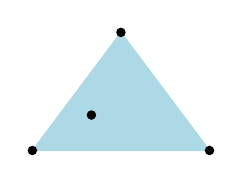
\begin{tikzpicture}[scale=1.5]
\coordinate (a) at (0,0);
\coordinate (b) at (1.5,0);
\coordinate (c) at (.75,1);

\coordinate (d) at (0.5,.3);
% \draw[green] (a) -- (d) --;
% \draw[blue] (b) -- (c);
\filldraw[LightBlue] (a) -- (b) -- (c) -- cycle;
\filldraw[black] (a) circle (1pt);
\filldraw[black] (b) circle (1pt);
\filldraw[black] (c) circle (1pt);
\filldraw[black] (d) circle (1pt);

\end{tikzpicture}
\hfill
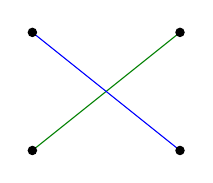
\begin{tikzpicture}[scale=1.5]
\coordinate (a) at (0,0);
\coordinate (b) at (0,1);
\coordinate (c) at (1.25,0);
\coordinate (d) at (1.25,1);
\draw[green] (a) -- (d);
\draw[blue] (b) -- (c);

\filldraw[black] (a) circle (1pt);
\filldraw[black] (b) circle (1pt);
\filldraw[black] (c) circle (1pt);
\filldraw[black] (d) circle (1pt);

% \node at (a) {\textbullet};

\end{tikzpicture}
\hfill
\caption{Four points in $\R^2$, when no three form a line. Either one is in the convex hull of the other three (left), or we may divide into pairs so that the convex hulls intersect (right).}\label{fig:Radon_example_d2}
\end{figure}
In either case, we may verify Radon's theorem.
% \missingfigure{BLue Triangle with dot in middle}
\end{remark}

\begin{proof}	
WLOG, we may take $|A|=d+2$; any surplus points we could put in $A_1,A_2$, or neither, without changing the result. Set $A=  \{v_1,v_2,\dotsc,v_{d+2}\}$. Since $v_1,v_2,\dotsc,v_{d+2}$ are affinely dependent\sidenote{since there are more than $d+1$ of them}, there exist $\alpha_1,\dotsc,\alpha_{d+2}$ with $\sum_i \alpha_i=0$ not all zero such that
\[
\alpha_1v_1 + \dotsb + \alpha_{d+2} v_{d+2} = 0.
\]
Let $A_1 = \{v_i : \alpha_i > 0\}$ and $A_2 = \{ v_i: \alpha_i < 0\}$. WLOG, $\alpha_1,\dotsc,\alpha_k > 0$ and $\alpha_{k+2},\dotsc,\alpha_{d+2} < 0$. Let $s = \alpha_1 + \dotsb + \alpha_k = - \alpha_{k+1} - \dotsb - \alpha_{d+2}$.
Then
\begin{align*}	
\left( \frac{\alpha_1}{s} \right) v_1 + \dotsb + \left( \frac{\alpha_k}{s} \right) v_{k+1} = \left( - \frac{\alpha_{k+1}}{s} \right)v_{k+1} + \dotsb + \left( - \frac{\alpha_{d+2}}{s} \right)v_{d+2}.
\end{align*}
But as shown by the LHS, this quantity lies in $\conv(A_1)$, and as shown by the RHS, the quantity lies in $\conv(A_2)$.
\end{proof}

\begin{theorem}[\cite{Caratheodory1911}]
Every point in $\conv(X)$ for $X\subset \R^d$ is a convex combination of at most $d+1$ points in $X$.
\end{theorem}
\begin{proof}	
Let $x\in \conv(X)$ be written $x = \alpha_1 v_1 + \dotsb + \alpha_n v_n$ for $v_1,\dotsc,v_n\in X$ and $\sum_i \alpha_i=0$ with $\alpha_i\geq 0$ not all zero. Suppose is $n$ is chosen minimally such that a convex combination exists. Suppose $n\geq d+2$ for the sake of contradiction. Then by Radon's theorem, wlog
\[
\conv(\{v_1,\dotsc,v_k\})\cap \conv(\{v_{k+1},\dotsc, v_n \}).
\]
So, for some $\beta_1,\dotsc,\beta_n\geq 0$,
\[
\beta_1 v_1 + \dotsb \beta_k v_k = \beta_{k+1} v_{k+1} + \dotsb + \beta_n v_n
\]
with $\sum_{i=1}^k \beta_i = \sum_{i=k+1}^n \beta_i = 1$. Then
\vspace{-\baselineskip}
\begin{fullwidth}
\begin{align}	
x &= (\alpha_1 + \epsilon \beta_1) v_1 + \dotsb + (\alpha_k + \epsilon \beta_k)v_k + (\alpha_{k+1} - \epsilon \beta_{k+1})v_{k+1}+ \dotsb +  (\alpha_n - \epsilon \beta_n)v_n \tag{$\star$} \label{eq:Cara_proof}
\end{align}
\end{fullwidth}
has the sum of coefficients one for every $\epsilon$. If $\epsilon>0$ is minimally such that $\alpha_i - \epsilon \beta_i=0$ for some $i$, then the expression \eqref{eq:Cara_proof} is a convex combination of $\{v_1,\dotsc,v_n\}\setminus \{v_i\}$, giving a contradiction.
\end{proof}
\begin{theorem}[\cite{Helly1923}]
Let $C_1,C_2\dotsc,C_n$ be a collection of convex sets in $\R^d$. If $\bigcap_{i\in I} C_i \neq \emptyset$ for every $I\subset [n]$ with $|I| = d+1$, then $\bigcap_{i=1}^n C_i \neq \emptyset$.
\end{theorem}
\begin{remark}
For $\R^1$, if we consider \marginnote{Convex sets in $\R^1$ may be open or closed intervals or rays, but we will take closed intervals for simplicity.}$C_i = [a_i,b_i]$, then if each $C_i\cap C_j\neq \emptyset$, then we need $a_i \leq b_j$ for each $i,j$. Then $[\max_i a_i, \min_i b_i] \subset C_k$ for all $k$.
\end{remark}
\begin{proof}[Proof by induction on $n$.] 
Let us postpone the base case, $n=d+2$.
For the induction step, let $C_1' = C_1 \cap C_n$, \ldots, $C_{n-1}' = C_{n-1} \cap C_n$. Then by the base case, any $(d+1)$ sets in $\{C_1',\dotsc,C_{n-1}'\}$ have a non-empty intersection. Therefore they all intersect by the induction hypothesis, hence
\[
\bigcap_{i=1}^n C_i = \bigcap_{i=1}^{n-1}C_i' \neq \emptyset.
\]
So let us show the base case. Let $v_i \in \bigcap_{j\neq i} C_j$; by the assumption. Let $A = \{v_1,\dotsc,v_{d+2}\}$. Then by Radon's theorem, there exist disjoint $A_1,A_2\subset A$ such that $\conv(A_1)\cap \conv(A_2)\neq \emptyset$. Consider $v\in \conv(A_1)\cap \conv(A_2)$. We will show that $v\in C_i$ for every $i$.

Suppose wlog that $v_i \in A_2$. Then $A_1 \subset C_i$. Since $C_i$ is convex, then $\conv(A_1) \subset C_i$. So $v\in C_i$, as desired. See \cref{fig:Helly_proof} for an example of this process in $\R^2$. \qedhere
% \missingfigure{Draw four disks in $\R^2$, $C_1,\dotsc,C_4$. Draw the $v_i$ in all the intersections but $v_i$. Connect $v_1,v_3$ in red $v_2,v_4$ in blue. Then let $v$ be the intersection. $v$ is in all four; it is in $C_1$ because it's in the interval between $v_2,v_4 \in C_1$. Etc.}
\begin{figure}
\begin{center}
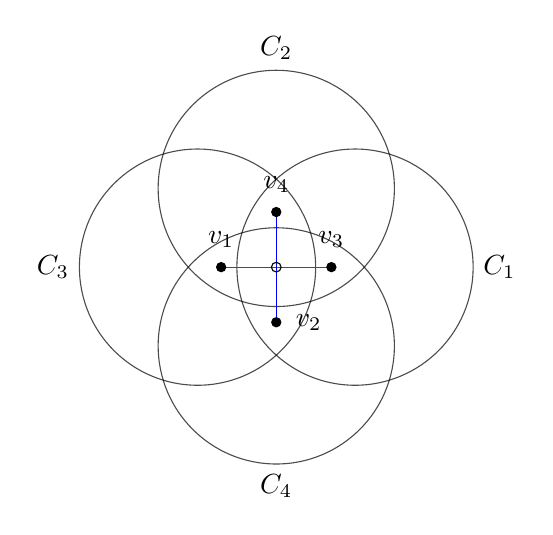
\begin{tikzpicture}[circ/.style={circle,minimum size=\circdiam cm,draw,opacity=.7}]


\def\circposrad{1}
\def\circdiam{3}

\node[circ,label={right:$C_1$}] at (0:\circposrad cm) {};
\node[circ,label={above:$C_2$}] at (90:\circposrad cm) {};
\node[circ,label={left:$C_3$}] at (180:\circposrad cm) {};
\node[circ,label={below:$C_4$}] at (270:\circposrad cm) {};

\coordinate (v3) at (0:.7cm);
\coordinate (v4) at (90:.7cm);
\coordinate (v1) at (180:.7cm);
\coordinate (v2) at (270:.7cm);

\draw[red] (-.7,0) -- (.7,0);
\draw[blue] (v2) -- (v4);

\filldraw[black] (v1) circle (1.65pt) node[label=$v_1$]{};
\filldraw[black] (v2) circle (1.65pt) node[label=right:$v_2$]{};
\filldraw[black] (v3) circle (1.65pt) node[label=$v_3$]{};
\filldraw[black] (v4) circle (1.65pt) node[label=above:$v_4$]{};

\draw (0,0) circle (1.75pt);% node[label={[label distance=.02cm]north east:$v$}]{};
\end{tikzpicture}
\end{center}
\caption{Helly's theorem in $\R^2$. Given four convex sets $C_1,\dots,C_4$ such that every triple has a non-empty intersection $v_i \in \bigcap_{j\neq i} C_j$, we can use Radon's theorem to divide $\{v_1,v_2,v_3,v_4\}$ into two disjoint sets with non-empty convex hull. Here, $A_1 = \{v_1,v_3\}$ and $A_2 = \{v_2,v_4\}$. The point in the intersection $\conv(A_1)\cap \conv(A_2)$ is labelled here with an open circle.} \label{fig:Helly_proof}
\end{figure}
\end{proof}

\begin{remark}
Helly's theorem may not apply to infinite collections of sets; consider $\{[n,+\infty):n\in \N\}$.
\end{remark}

For any set of $n$ points on the line, we can find a point such that there are at least $n/2$ points above it and below it. This is the median. How do we find an analog for $\R^d$? We'd like to find a point that in any direction away from this point, there are still many points in our set.


Let us generalize to $\R^d$: Given $X\subset \R^d$, $|X|=n$, the \defn{centerpoint} of $x$ is a point $m\in \R^d$ such that for every closed halfspace $H\subset \R^d$ such that $m\in H$, then $H$ contains at least $\frac{n}{d+1}$ points in $X$.

\begin{theorem}
For every finite set $X\subset \R^d$, there exists a centerpoint.
\end{theorem}
\begin{proof}	
Note the following are all equivalent:
\begin{itemize}
\item $m$ is a centerpoint
	\item  For every closed halfspace $H\subset \R^d$, if $m\in H$ then $|H\cap X| \geq \frac{n}{d+1}$.
	\item For every closed halfspace $H\subset \R^d$, if  $|X\cap H| < \frac{n}{d+1}$, then $m\not \in H$.
	\item For every closed halfspace $H\subset \R^d$, if $|X\cap H^c| > n - \frac{n}{d+1} = \frac{dn}{d+1}$, then $m\in H^c$.
	\item For every open halfspace $H\subset \R^d$, if $|X\cap H| >  \frac{dn}{d+1}$, then $m\in H$.
\end{itemize}
% Alternatively, every open half space which does not contain $m$ must contain at most $$
Consider the family 
\begin{align*}	
\H = \{H: H \text{ is an open halfspace of }\R^d, |H\cap X| >  \frac{dn}{d+1}\}.
\end{align*}
We will show for some $m \in \R^d$, we have $m\in H$ for every $H\in \H$, proving that $m$ is a centerpoint. 
First, if $H_1,H_2,\dotsc,H_{d+1}\in \H$, then
\begin{align*}	
H_1\cap H_2\cap \dotsm \cap H_{d+1}\neq \emptyset.
\end{align*}
Otherwise, every point of $X$ belongs to $\leq d$ out of $d+1$ of these half spaces, and thus
\begin{align*}	
dn = \sum_{i=1}^{d+1} \frac{dn}{d+1} < \sum_{i=1}^{d+1} |H_i \cap X| \leq d n
\end{align*}
which is a contradiction.

We would like to now apply Helly's theorem, but we have an infinite collection $\H$ instead of a finite one.

Let us instead set $\H' = \{ \conv(Y): Y\subset X, |Y| > \frac{dn}{d+1}\}$. By the previous argument and Helly's theorem, there exists $m\in \R^d$ such that $m\in C$ for every $C\in \H'$. But this suffices. For any $H\in \H$  there is $Y\subset X$ with $|Y| > \frac{dn}{d+1}$ and $Y\subset H$. Then $\conv(Y) \subset H$ since $H$ is convex. But since $m\in \conv(Y)$, we have $m\in H$, as desired.%if $m\not \in H$, then $m\not \in \conv(Y)$ which is a contradiction.
% If $m\not \in H$, then we want that $H$ contains
\end{proof}



\begin{theorem}[Birch]
Let $X\subset \R^2$ be a collection of $3n$ points. Then $X$ can be partitioned into $n$ triples such that the corresponding triangles all share a point in common.
\end{theorem}

\begin{figure}
\begin{center}
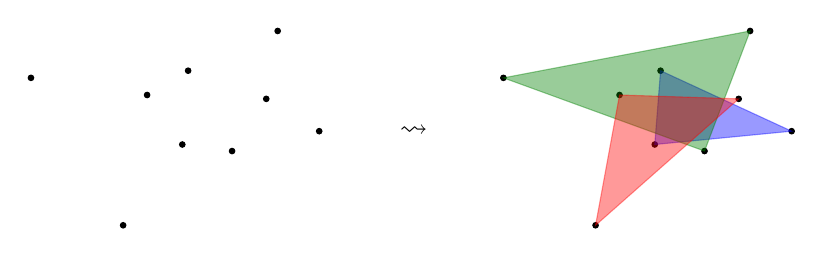
\begin{tikzpicture}
\begin{scope}[scale=.6]
\coordinate (v1) at (0:3cm);
\coordinate (v9) at (20:2cm);
\coordinate (v6) at (130:1cm);
\coordinate (v3) at (240:2.3cm);
\coordinate (v5) at (160:3.3cm);
\coordinate (v4) at (290:.3cm);
\coordinate (v7) at (80:1.3cm);
\coordinate (v2) at (340:1.23cm);
\coordinate (v8) at (45:3cm);
\foreach \n in {1,2,3,4,5,6,7,8,9}
{
	\filldraw (v\n) circle (1.65pt);
}
\end{scope}
\node at (3cm,0){$\leadsto$};
\begin{scope}[scale=.6, xshift=10cm]
\coordinate (v1) at (0:3cm);
\coordinate (v9) at (20:2cm);
\coordinate (v6) at (130:1cm);
\coordinate (v3) at (240:2.3cm);
\coordinate (v5) at (160:3.3cm);
\coordinate (v4) at (290:.3cm);
\coordinate (v7) at (80:1.3cm);
\coordinate (v2) at (340:1.23cm);
\coordinate (v8) at (45:3cm);
\foreach \n in {1,2,3,4,5,6,7,8,9}
{
	\filldraw (v\n) circle (1.65pt);
}

\filldraw[blue,opacity=.4] (v7) -- (v4) -- (v1) -- cycle;

\filldraw[green,opacity=.4] (v2) -- (v5) -- (v8) -- cycle;

\filldraw[red,opacity=.4] (v3) -- (v6) -- (v9) -- cycle;
\end{scope}


\end{tikzpicture}
\end{center}
\caption{An example of Birch's theorem with nine points. On the left, the nine points are depicted; on the right, intersecting triangles chosen.}\label{fig:birch_ex}
\end{figure}
% \missingfigure{Draw 9 points and three triangles in different colors so that there is a common area. Label a point of intersection.}
\begin{remark}
See \cref{fig:birch_ex} for an example.
\end{remark}\begin{proof}
% \missingfigure{Draw rays from centerpoint to each vertex}

Let $m$ be a centerpoint of $X$. Label the points of $X$ by $x_1$, $x_2$, \ldots, $x_{3n}$ so that the rays $mx_1$, $mx_2$, \ldots, $mx_{3n}$ are arranged around $m$ in clockwise order, as shown in \cref{fig:birch_proof1}.
\begin{figure}[ht]
\begin{center}
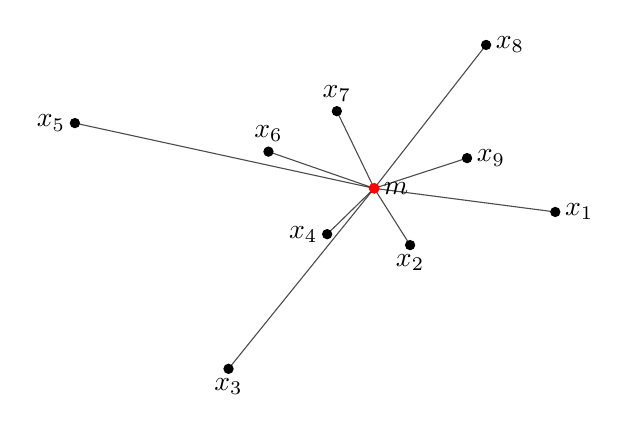
\begin{tikzpicture}
\begin{scope}[scale=1]
\coordinate (m) at (.7cm,.3cm);
\coordinate (v1) at (0:3cm);
\coordinate (v9) at (20:2cm);
\coordinate (v6) at (130:1cm);
\coordinate (v3) at (240:2.3cm);
\coordinate (v5) at (160:3.3cm);
\coordinate (v4) at (290:.3cm);
\coordinate (v7) at (80:1.3cm);
\coordinate (v2) at (340:1.23cm);
\coordinate (v8) at (45:3cm);
\foreach \n in {6,7}
{
	\filldraw (v\n) circle (1.65pt) node[above]{$x_\n$};
}
\foreach \n in {4,5}
{
	\filldraw (v\n) circle (1.65pt) node[left]{$x_\n$};
}
\foreach \n in {1,8,9}
{
	\filldraw (v\n) circle (1.65pt) node[right]{$x_\n$};
}
\foreach \n in {2,3}
{
	\filldraw (v\n) circle (1.65pt) node[below]{$x_\n$};
}

% \filldraw[blue,opacity=.4] (v5) -- (v4) -- (v1) -- cycle;

% \filldraw[green,opacity=.4] (v3) -- (v9) -- (v8) -- cycle;

% \filldraw[red,opacity=.4] (v6) -- (v7) -- (v2) -- cycle;

	\foreach \n in {1,2,...,9}
{
	\draw[opacity=.7] (m) -- (v\n);
}
	\filldraw[red] (m) circle (1.75pt) node[black,right]{$m$};

\end{scope}
\end{tikzpicture}
\end{center}
\caption{Nine points $\{x_1,\dotsc,x_9\}$ in $\R^2$ and their centerpoint $m$, in red. Continuing the example from \cref{fig:birch_ex}, the points are labelled clockwise in order from the centerpoint. }\label{fig:birch_proof1}
\end{figure}
Let $X_i = \{ x_i, x_{i+n}, x_{i+2n}\}$ for $i=1,\dotsc, n$. Then $m\in \conv(X_i)$ for each $i$.

Assume $m\not \in \conv(X_i)$. Then\sidenote{We are appealing to a separating hyperplane theorem, such as \cite[Theorem 1.24]{matouvsek2002lectures}, although the result seems clear geometrically in this case.} some closed halfplane containing $m$ separates $m$ from the three points of $X_i$; see \cref{fig:birch_proof2}. But then the $2n$ rays between $x_i$ and $x_{i+2n}$ fall in the other half of the halfplane, so there are at least $2n+1$ points in $X$ on the other side, contradicting that $m$ is a centerpoint. \qedhere
\begin{marginfigure}
\begin{center}
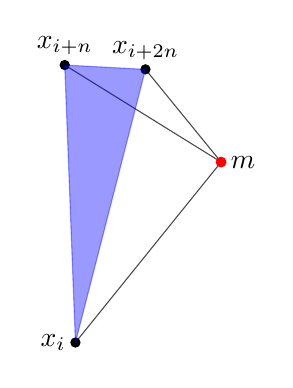
\begin{tikzpicture}
\coordinate (v3) at (240:2.3cm);
\coordinate (v2) at (100:1.5cm);
\coordinate (v1) at (130:2cm);
\coordinate (m) at (.7cm,.3cm);
\foreach \n in {1,2,3}
{
	\draw[opacity=.7] (m) -- (v\n);
}
	\filldraw (v3) circle (1.65pt) node[left]{$x_i$};
	\filldraw (v2) circle (1.65pt) node[above]{$x_{i+2n}$};
	\filldraw (v1) circle (1.65pt) node[above]{$x_{i+n}$};


\filldraw[blue,opacity=.4] (v1) -- (v2) -- (v3) -- cycle;
	\filldraw[red] (m) circle (1.75pt) node[black,right]{$m$};

\end{tikzpicture}

\end{center}
\caption{The case where the centerpoint $m$, in red, is not in the convex hull of $X_i$, shown in blue. Then the $2n$ points $\{x_i,x_{i+1},\dotsc,x_{i+2n}$ all lie between $x_i$ and $x_{i+2n}$ (angularly) and may be separated from $m$ by a closed hyperplane, contradicting the definition of centerpoint.} \label{fig:birch_proof2}
\end{marginfigure}
% \missingfigure{$m$, then line, and three points $x_i$, $x_{i+n}$, $x_{i+2n}$. Draw outline convex hull in red  around those three. They are all on the other side of a halfplane from $m$.}

\end{proof}

\begin{theorem}[Colorful Carath\'eodory theorem, \cite{barany1982generalization}]
Let $S_1,S_2,\dotsc,S_{d+1}\subset \R^d$ and suppose that $x\in \bigcap_{i=1}^{d+1} \conv(S_i)$. Then there exist $x_1\in S_1$, $x_2\in S_2$, \ldots, $x_{d+1}\in S_{d+1}$ such that $x\in \conv(\{x_1,x_2,\dotsc,x_{d+1}\})$.
\end{theorem}
\begin{remark}
The different sets correspond to different colors. Then $x$ belongs to a convex combination of points each a different color. Taking each set $S_i \equiv X$, we recover Carath\'eodory's theorem.
\end{remark}
\begin{proof}	
We will say $C$ is a \defn{colorful simplex} if $C = \conv(\{ x_1,x_2,\dotsc,x_{d+1} \})$ for $x_i\in S_i$ for $i\in[d+1]$. Suppose that no colorful simplex contains $x$.

Choose a colorful simplex $C$ such that $\dist(C,x) = \min_{c\in C} \|c-x\|$ is minimal.\marginnote{$\|c-x\| = \dist(c,x)$ is the 2-norm (Euclidean norm).}

Let $z\in C$ be the closest point to $x$: $\dist(z,x) = \dist(C,x)$.


Let $H$ be a hyperplane orthogonal to $zx$ through $z$. Let $H^+$ and $H^-$ be closed halfspaces with respect to $H$ such that $x\in H^-$.

\begin{claim}
$C\subset H^+$.
\end{claim}
\begin{subproof}	
Suppose not: $z' \in C\cap (H^- \setminus H^+)$\marginnote{So $z'\not \in H^+$}. Then angle $z' z x$ is acute and points on $zz'$ near $z$ are closer to $x$ than $z$, a contradiction.
\end{subproof}

\begin{claim}
$z\in \conv(\{x_1,\dotsc,x_{d+1}\}\cap H)$.
\end{claim}
\begin{subproof}	
$z = \sum_{i=1}^{d+1} \lambda_i x_i$ with $\lambda_i\geq 0$, $\sum_i \lambda_i =1$, since $z\in C$. Let $f: \R^d \to \R$ linear such that if $f(p)> 0$ for $p\in H^+\setminus H$, and $f(p) = 0$ for $p\in H$. 

Then $0 = f(z) = \sum_{x_i \in H^+ \setminus H} \lambda_i \underbrace{f(x_i)}_{>0} + \sum_{x_i \in H} \lambda_i \underbrace{f(x_i)}_{=0}$. So we must have $\lambda_i=0$ when $x_i \in H^+ \setminus H$.
\end{subproof}

By Caratheordy theorem applied to $z$ and $\{x_i,\dotsc,x_{d+1}\}\cap H$, there exists $j$ such that \begin{align*}	
z\in \conv((\{x_1,x_2,\dotsc,x_{d+1}\}\setminus \{j\})\cap H).
\end{align*}
We know $x\in \conv(S_j)$, so there exists $x'_j \in S_j \cap (H^-\setminus H^+)$. Let $C' = \conv( \{x_1,\dotsc,x_{j-1},x_j',x_{j+1},\dotsc,x_{d+1}\})$.

\begin{claim}
Then $\dist(C',x) < \dist(C,x)$.
\end{claim}
\begin{subproof}	
We know $z\in C'$. Then, as before, points on $x_j' z\subset C'$ are closer to $x$ than $z$. 
\end{subproof}
This last claim yields a contradiction to minimality of $C$.

Note: we assumed the $S_i$ were finite when assuming there exists a minimal colorful simplex $C$. But in fact, we only need to consider $\conv(S_i)$, which only depends on $d+1$ points, by (the original) Carath\'eodory points. Thus, we could take $|S_i|=d+1$ for each $i$.
\end{proof}
\begin{remark}
This proof yields an algorithm to improve our convex set one point at a time to the optimal one. Yet, it is unknown if this algorithm or any other can find the optimal $\conv(\{x_1,\dotsc,x_{d+1}\})$ in polynomial time.
\end{remark}

\begin{theorem}[\cite{Tverberg1966}]
Let $A\subset \R^d$ with $|A| \geq (r-1)(d+1)+1$. Then there exist $A_1,A_2,\dotsc,A_r\subset A$ pairwise disjoint such that $\bigcap_{i=1}^r \conv(A_i)\neq \emptyset$.
\end{theorem}
\begin{remark}
Radon's theorem is the case $r=2$. If $d=1$, then we have $2r-1$ points in $\R$ which we wish to write as $r$ groups with intersecting convex hulls.

For $d=2$, $3r-2$ points in $\R^2$ can be partitioned into $r$ groups with intersecting convex hulls. This in fact implies Birch's theorem.
\end{remark}

If $u\in \R^n$ and $v\in \R^m$, then $u\otimes v \in \R^{nm}$. Suppose $u = (u_1,\dotsc,u_n)$ and $v = (v_1,\dotsc,v_m)$; i.e., we have chosen bases for $\R^n$ and $\R^m$. Then $u\otimes v $ can be thought of as a $m\times n$ matrix with components $(u\otimes v)_{ij} = u_i v_j$.
\begin{align*}	
u = \begin{pmatrix}
u_1\\ u_2\\ u_3
\end{pmatrix}, \qquad v = \begin{pmatrix}
v_1 \\ v_2 \\ v_3
\end{pmatrix}, \qquad u\otimes v = \begin{pmatrix}
u_1 v_1 & u_1 v_2 & u_1 v_3\\
u_2 v_1 & u_2 v_2 & u_2 v_3 \\
u_3 v_1 & u_3 v_2 & u_3 v_3
\end{pmatrix}.
\end{align*}

\begin{proposition}
~\begin{enumerate}
\item $(\alpha_1 u_1 + \alpha_2 u_2) \otimes v = \alpha_1 (u_1\otimes v) + \alpha_2 (u_2\otimes v)$
\item  Suppose $v_1,\dotsc,v_k$ are linearly independent and $u_1\otimes v_1 + u_2\otimes v_2 + \dotsm + u_k \otimes v_k = 0$. Then $u_1 = u_2 = \dotsm = u_k = 0$.
\end{enumerate}
\end{proposition}
We will leave the proof of the proposition as an exercise, and proceed to the proof of Tverberg's theorem.
\lect{3}{23}
% \marginnote{Lecture X: March 23, 2016.}

\begin{proof}[Proof (\cite{sarkaria1992tverberg}).]
Let $m = (r-1)(d+1)+1$.

\begin{enumerate}
	\item Instead of the orginal setting, consider $A = \{v_1,v_2,\dotsc,v_m\} \subset \R^{d+1}$ such that the vectors of $A$ lie in an affine hyperplane not passing through the origin. I.e., there exists $f: \R^{d+1}\to \R$ linear such that $f(v_i) = 1$ for every $i$. 
	\item Let $w_1,w_2,\dotsc,w_r$ be vectors in $\R^{r-1}$ such that $w_1+w_2+\dotsc+w_r=0$ and this is essentially the only relation between these vectors. For instance, we could choose $w_i = (\underbrace{0,\dotsc,0}_{i-1},1,0,\dotsc,0)$ for $i=1,\dotsc,r-1$ and $w_r = (-1,-1,\dotsc,-1)$.
	\item Consider $\{v_i \otimes w_j: 1\leq i \leq m, 1\leq j \leq r\}\subset \R^{d+1}\otimes \R^{r-1}\cong \R^{m-1}$. For each $i$, we may think of $S_i:=\{v_i\otimes w_j:1\leq j\leq r\}$ as a copy of the $w_j$ embedded in a hyperplane. Note $0\in \conv(S_i)$ for each $i$, since
	\begin{align*}	
	0 &= \frac{1}{r}v_i \otimes (w_1+w_2+\dotsm+ w_r) = \frac{1}{r} v_i \otimes w_1 + \frac{1}{r}v_i\otimes w_2  +\dotsm + \frac{1}{r}v_i\otimes w_r.
	\end{align*}
	\item Apply the Colorful Carath\'eodory theorem to $S_1,\dotsc,S_m$ and the point $0$. We get that for $1\leq i\leq m$ there exist $j_i$ and $\lambda_i\geq 0$ such that
	\begin{align}	
	\sum_{i=1}^m \lambda_i (v_i\otimes w_{j_i})=0 \label{eq:Tv_conv_comb}
	\end{align}
	with $\sum_i \lambda_i=1$.

	Let $A_j = \{ v_i : j_i = j \}$ for $j=1,\dotsc,r$. Let us rewrite \cref{eq:Tv_conv_comb} as follows.
	\begin{align*}	
	\sum_{j=1}^r \left( \sum_{v_i \in A_j} \lambda_i v_i \right)\otimes w_j = 0.
	\end{align*}
	Let us write $u_j =  \sum_{v_i \in A_j} \lambda_i v_i$. Then we have
	\begin{align*}	
	u_1\otimes w_1 + u_2\otimes w_2 + \dotsm + u_r\otimes w_r &= 0\\
	(u_1- u_r)\otimes w_1 + (u_2-u_r)\otimes w_2 + \dotsm + (u_{r-1} - u_r)\otimes w_{r-1} &= 0
	\end{align*}
	using $w_r = -w_1 - w_2 - \dotsm - w_{r-1}$. But since $\{w_1,\dotsc,w_{r-1}\}$ are linearly independent, we must have $u_1-u_r = u_2 - u_r = \dotsm = u_{r-1}- u_r = 0$. That is, 
	\[
	u_1 = u_2 = \dotsm = u_r.
	\]
	Substituting the definition of $u_j$,
	\begin{align}	
	\sum_{v_i \in A_1} \lambda_i v_i = \sum_{v_i\in A_2} \lambda_i v_i = \dotsm = \sum_{v_i\in A_r}\lambda_i v_i. \label{eq:Tv_lambda_vs_equal}
	\end{align}
	Suppose the sum of coefficients $\lambda_i$ in each expression is the same and is equal to $s$.\marginnote{In fact, $s= \frac{1}{r}$.} Then
	\begin{align*}	
	\sum_{v_i \in A_1} \frac{\lambda_i}{s}v_i = \dotsm = \sum_{v_i\in A_r} \frac{\lambda_i}{s}v_i = p
	\end{align*}
	and hence $p\in \conv(A_k)$.

	But if we apply $f$ to \cref{eq:Tv_lambda_vs_equal}, by linearity we obtain
	\begin{align*}	
	\sum_{v_i \in A_1} \lambda_i f(v_i) = \sum_{v_i\in A_2} \lambda_i f(v_i) = \dotsm = \sum_{v_i\in A_r}\lambda_i f(v_i). 
	\end{align*}
	Since $f(v_i)=1$ for all $i$, we find $\sum_{v_i\in A_j} \lambda_i \equiv s$. \qedhere
\end{enumerate}
\end{proof}
\flavor{A magical proof. 30 years after the original.}

\begin{remark}
In Helly's theorem, we consider $C_1,\dotsc,C_n\subset \R^d$ convex such that every $(d+1)$-tuple of $C$'s has non-empty intersection. Then we obtain that there is a common point in all of the sets. Suppose instead $\sim \frac{1}{2}$ of the $(d+1)$-tuples have a non-empty intersection. What can we say about large intersections?
\end{remark}
\begin{theorem}[Fractional Helly's theorem]
For every $d\in \N$ and $0< \alpha \leq 1$ there exists a $\beta = \beta(\alpha,d)$ such that the following holds. Let $C_1, C_2,\dotsc,C_n\subset \R^d$ be convex and suppose $\bigcap_{i\in I} C_i\neq \emptyset$ for at least $\alpha {n\choose d+1}$ sets $I\subset[n]$ with $|I| = d+1$. Then there exists $X \subset [n]$ with $|X|\geq \beta n$ such that $\bigcap_{i\in X} C_i \neq \emptyset$.

\end{theorem}
\begin{proof}	
We need to assume that $C_1,C_2,\dotsc,C_n$ are compact; we may do this as follows. For each set $I$ as in the statment, select $p_I \in \bigcap_{i\in I} C_i$. Then replace $C_i$ by $\conv(\{p_I:  I \text{ s.t. } I\ni i\})$.

Let $F_I = \bigcap_{i\in I} C_i$. Let $<$ be a linear lexicographic order on $\R^d$. Let $p_I= \min (F_I)$ in this order, if $F_I\neq \emptyset$. Since $F_I$ is compact, $p_I$ exists and is unique.

\begin{claim}
For every $I\subset[n]$ with $|I|=d+1$, s.t. $F_I\neq \emptyset$, there exists $J\subset I$, $|J| = d$ such that $p_I = p_J$.
\end{claim}
\begin{remark}
For any $J\subset I$,  we have $p_J \leq P_I$.
\end{remark}
\begin{subproof}[Proof of claim.]
Let $C =  \{q \in \R^d: q< p_I\}$. Then $C$ is convex. Then $C\cap \left( \bigcap_{i\in I} C_i \right) = C\cap F_I = \emptyset$. Since this $(d+2)$-tuple intersection is empty, then by the contrapositive of Helly's theorem, not all $(d+1)$-tuples can have empty intersection. But since $F_I\neq \emptyset$, the $(d+1)$-tuple with empty intersection must include $C$. So there exists $J\subset I$ with $|J| = d$ such that
\begin{align*}	
C \cap \left( \bigcap_{i\in J}C_i \right) = \emptyset.
\end{align*}
Then $p\geq p_I$ for every $p\in F_J$.
\end{subproof}

Now for every $I\subset[n]$ with $|I| = d+1$, $F_I\neq \emptyset$, select $J\subset I$ with $|J| = d$ such that $P_J = P_I$. Then there are $\alpha{n \choose d+1}$ sets $I$ which we consider, and  ${n\choose d}$ sets $J$ of size $d$. So some set $J_0$ is associated with at least $\frac{\alpha {n\choose d+1}}{{n\choose d}}$ sets $I$. Such sets are of the form $J_0 \cup \{ i\}$ for some $i$, and $p_{J_0} \in C_i$ for such $i$. So $p_{J_0}$ belongs to  at least 
\begin{align*}	
\frac{\alpha{ n\choose d+1}}{{n\choose d}} + d = \frac{\alpha(n-d)}{d+1}+d \geq \frac{\alpha}{d+1}n
\end{align*}
sets $C_i$ (counting the $d$ sets in $J_0$).
Therefore, we may take $\beta = \frac{\alpha}{d+1}$.
\end{proof}
\begin{remark}
This constant is not optimal; for instance, when $\alpha=1$, we would like $\beta=1$ to recover Helly's theorem. The optimal constant is known, however.
\end{remark}


For every $k$, we'd like to prove existence (and estimate the value) of the number $g(k)$ such that in every set of $g(k)$ points in $\R^2$, with no three lying on a line\sidenote[][-1cm]{``in general position''} there exist $k$ points which are convexly independent\sidenote[][-1cm]{``in convex position,'' or are the verticies of a convex polygon}.

Let us consider small $k$. Then $g(1)=1$, $g(2)=2$, $g(3)=3$. But $g(4) > 4$, as shown in \cref{fig:g4}.
\begin{marginfigure}[-1cm]
\begin{center}
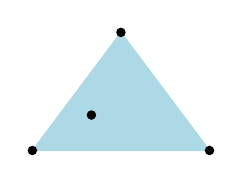
\begin{tikzpicture}[scale=1.5]
\coordinate (a) at (0,0);
\coordinate (b) at (1.5,0);
\coordinate (c) at (.75,1);

\coordinate (d) at (0.5,.3);
% \draw[green] (a) -- (d) --;
% \draw[blue] (b) -- (c);
\filldraw[LightBlue] (a) -- (b) -- (c) -- cycle;
\filldraw[black] (a) circle (1pt);
\filldraw[black] (b) circle (1pt);
\filldraw[black] (c) circle (1pt);
\filldraw[black] (d) circle (1pt);

\end{tikzpicture}
\end{center}
\caption{An illustration of the fact that $g(4) > 4$. We have four points with no three lying on a line such that not all four are convexly independent: one point is in the convex hull of the other three.} \label{fig:g4}
\end{marginfigure}

\begin{lemma} \label{lem:g4_is_5}
$g(4)=5$.
\end{lemma}
\begin{proof}	
Let $X\subset \R^2$ be a set of five points in general position. Consider $\conv(X)$: this is a polygon with 3, 4, or 5 vertices. If there are 4 or 5 vertices we are done, so, assume $\conv(X)$ is a triangle with vertices $\{a,b,c\}$. Let $\{d,e\}$ be the remaining two points of $X$, as shown in \cref{fig:lem89convX}.
\begin{figure}
\begin{center}
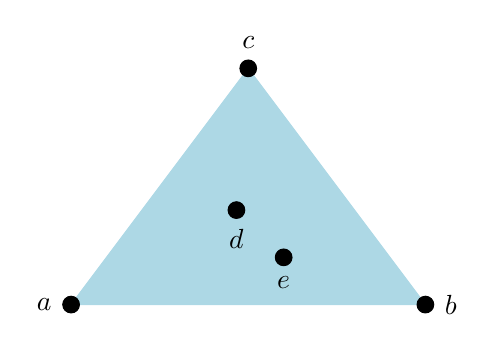
\begin{tikzpicture}[scale=3]
\coordinate (a) at (0,0);
\coordinate (b) at (1.5,0);
\coordinate (c) at (.75,1);

\coordinate (e) at (0.9,.2);
\coordinate (d) at (0.7,.4);

% \draw[green] (a) -- (d) --;
% \draw[blue] (b) -- (c);
\filldraw[LightBlue] (a) -- (b) -- (c) -- cycle;
	\filldraw[black] (a) circle (1pt) node[label=left:$a$]{};
\filldraw[black] (b) circle (1pt)node[label=right:$b$]{};
\filldraw[black] (c) circle (1pt)node[label=above:$c$]{};
\filldraw[black] (d) circle (1pt)node[label=below:$d$]{};
\filldraw[black] (e) circle (1pt)node[label=below:$e$]{};

\end{tikzpicture}
\end{center}
\caption{We assume $\conv(X) = \conv(\{a,b,c\})$; then $\{d,e\}:= X\setminus \{a,b,c\}$ lie inside the triangle formed by $\{a,b,c\}$.} \label{fig:lem89convX}
\end{figure}

Now assume the line $de$ intersects $ab$ and $ac$, as shown in \cref{fig:lem89de_line}.
\begin{marginfigure}
\begin{center}
\usetkzobj{all}
\begin{tikzpicture}[scale=1.5]
\coordinate (a) at (0,0);
\coordinate (b) at (1.5,0);
\coordinate (c) at (.75,1);

\coordinate (e) at (0.9,.2);
\coordinate (d) at (0.6,.4);

% \draw[green] (a) -- (d) --;
% \draw[blue] (b) -- (c);
\filldraw[LightBlue] (a) -- (b) -- (c) -- cycle;
	\filldraw[black] (a) circle (1pt) node[label=left:$a$]{};
\filldraw[black] (b) circle (1pt)node[label=right:$b$]{};
\filldraw[black] (c) circle (1pt)node[label=above:$c$]{};
\filldraw[black] (d) circle (1pt)node[label=below:$d$]{};
\filldraw[black] (e) circle (1pt)node[label=below:$e$]{};



  % \tkzDefLine[through d](d,e)
  \tkzDrawLine[add = 2 and 2](d,e)
\end{tikzpicture}
\end{center}
\caption{We assume the line passing through $d$ and $e$ intersects the sides $ac$ and $ab$ of the triangle. Since no three points in $X$ are colinear, the line passing through $d$ and $e$ must intersect two of the sides of the triangle, so we can always relabel the verticies so that this is the case.} \label{fig:lem89de_line}
\end{marginfigure} Then $bcde$ form a convex quadrangle. We may see this by taking the convex hull of any three of $\{b,c,d,e\}$ to form a triangle $T$, and calling the omitted point $z$. Then there are two boundary line segments of the quadrilateral $bcde$ which end in $z$, but each of these line segments only intersects $T$ at the opposite end from $z$. If $z\in T$, then the whole line between $z$ and those endpoints would have to be included in $T$. Thus, $z\not \in T$, and we truly have a convex quadrilateteral $bcde$. This is illustrated in \cref{fig:lem89T}.
\begin{figure}
\begin{center}
\begin{tikzpicture}[scale=3]
\coordinate (a) at (0,0);
\coordinate (b) at (1.5,0);
\coordinate (c) at (.75,1);

\coordinate (e) at (0.9,.2);
\coordinate (d) at (0.7,.4);

% \draw[green] (a) -- (d) --;
% \draw[blue] (b) -- (c);
\filldraw[LightBlue] (a) -- (b) -- (c) -- cycle;
	\filldraw[black] (a) circle (1pt) node[label=left:$a$]{};
\filldraw[black] (b) circle (1pt)node[label=right:$b$]{};
\filldraw[black] (c) circle (1pt)node[label=above:$c$]{};
\filldraw[black] (d) circle (1pt)node[label=below:$d$]{};
\filldraw[black] (e) circle (1pt)node[label=below:$e$]{};

\filldraw[pattern=north west lines] (c) -- (d) -- (b) -- cycle;

\draw[dashed] (d)--(e);
\draw[dashed] (e)--(b);

\end{tikzpicture}
\end{center}
\caption{We will take $T= \conv(\{c,d,b\})$, the crosshatched region. Then the two dashed lines only intersect $T$ at the verticies $d,b$. We see if $e$ were moved up into $T$, then the line passing through $d$ and $e$ would no longer intersect the segment $ab$.} \label{fig:lem89T}
\end{figure}
\end{proof}
\begin{theorem}[\cite{erdosszekeres1935combinatorial}]
$g(k)$ exists for all $k$.
\end{theorem}
\begin{proof}	
Let $n=g(k)$ be such that in every coloring of $[n]^{(4)}$ in colors red and blue, one can find either a set of $5$ with all quadruples in red, or a set of size $k$ with all quadruples blue. This exists by the Hypergraph Ramsey theorem\sidenote{For all positive integers $r,k_1$, and $k_2$ there exists a positive integer $n= R^{(r)}(k_1,k_2)$ so that the following holds. If elements of $[n]^{(r)}$ are colored in colors red and blue then there is a set $Z\subset [n]$ such that either $|Z| = k_1$ and all elements of $Z^{(r)}$ are red, or $|Z| = k_2$ and all elements of $Z^{(r)}$ are blue.}.

Color quadruples of points in red color if it is not in convex position, and otherwise in blue. By  \cref{lem:g4_is_5}, there exists a set of $k$ points such that every four of them are in convex position.

Then these $k$ points are in convex position by Carath\'eodory's theorem.
\end{proof}
\begin{remark}
We may obtain much better bounds by longer proofs.
\end{remark}


\begin{fullwidth}
\printbibliography[segment=\therefsegment,heading=subbibliography]
\end{fullwidth}


\clearpage
\newrefsegment
%!TEX root = ../CombinatoricsNotes.tex

\section{Incidence problems}
\lect{4}{4}
% \marginnote{Lecture X: Monday, April 4, 2016.}
\begin{theorem}[Euler's formula]
Let $G$ be a connected graph drawn in the plane without crossings. Then
\[
|V(G)| - |\edges (G)| + \reg (G) =2
\]
where $\reg (G)$ is the number of regions in which the drawing divides the plane.
\end{theorem}

\begin{corollary} \label{cor:bound_edges_of_planar_3VG}
Let $G$ be a graph drawn in the plane without crossings. Then
\[
|\edges (G) |\leq 3 |V(G)|.
\]
\end{corollary}
\begin{proof}	
We assume $|V(G)|\geq 3$. By adding additional edges we can ensure that each region of the drawing has a cycle of length 3 as its boundary. Then
\[
3 \reg(G) = 2 |\edges (G)|
\]
by double counting pairs (edge, region) such that each edge belongs to two regions boundary. Substituting into Euler's formula, we have 
\[
|V(G)| - |\edges (G)| + \frac{2}{3}|\edges (G)| = 2
\]
so
\[
|\edges (G)| = 3 | V(G)| - 6 \leq 3 |V(G)|.
\]
\end{proof}

Let $\crossings(G)$ denote the minimal number of pairs of crossing edges taken over all drawing of $G$ in the plane  where vertices are represented by points, edges by curves joining corresponding points, and the drawing of edges are allowed to intersect, and each intersection is a \emph{crossing}\sidenote{locally looks like an $X$, not two curves bouncing off each other.}.

Then $\crossings(G)=0$ iff $G$ can be drawn in the plane without crossings, and $\crossings(K_5)=1$, by the drawing
\begin{center}
\begin{tikzpicture}

\end{tikzpicture}
\end{center}


\begin{corollary} \label{cor:bound_crossings_planar_graph93}
$\crossings(G) \geq |\edges (G)| - 3 |V(G)|$.
\end{corollary}
\begin{proof}	
Let $G$ be a graph with $\crossings(G) = c$. In a drawing of $G$ with $c$ pairs of crossing edges, remove $c$ edges to obtain a graph drawin without crossings. Then by \cref{cor:bound_edges_of_planar_3VG},
\[
|\edges (G)| - c \leq 3 |V(G)|
\]
as we wanted.
\end{proof}

\begin{theorem}[Crossing number lemma]
\label{thm:crossing_number_lemma}

\[
\crossings(G) \geq \frac{1}{64}\frac{m^3}{n^2}
\]
for every graph $G$ with $m$ edges and $n$ vertices such that $m\geq 4n$.
\end{theorem}
\begin{proof}	
Let $p \in [0,1]$ which we will choose later. Let $X\subset V(G)$ be obtained by choosing to include each vertex independently at random with probability $p$. Let $G'$ be the random subgraph of $G$ induced by $X$, namely $V(G') = X$, $\edges(G') = \edges(G| X)$. Let $m = |\edges(G)|$, $n= |V(G)|$, $x= \crossings(G)$, $m' = |\edges(G')|$, $n' = |V(G')|$, $x' = \crossings(G')$. Then by construction $\E[n'] = np$. Since each edge of $G$ survives with probability $p^2$, by linearity $\E[m']= mp^2$. Next, $\E[x'] \leq xp^4$ because the probability that a particular pair of crossing edges survives is $p^4$.

By \cref{cor:bound_crossings_planar_graph93}, $x'\geq m' - 3n'$. Taking expectation values, we have the bound $x p^4 \geq mp^2 - 3np$. That is,
\[
x\geq \frac{m}{p^2} - 3 \frac{n}{p^3}.
\]
Now, we choose optimal $p$:
\begin{gather*}
 \frac{\partial}{\partial p} \left( \frac{m}{p^2}- \frac{3n}{ p^3} \right) = - \frac{2m}{p^3} + \frac{9n}{p^4} = 0 \\
 \implies p=\frac{1}{4.5}\frac{n}{m}.
\end{gather*}
Let us simply take $p = \frac{1}{4}\frac{n}{m}.$ Then
\begin{gather*}
\crossings (G):=x \geq \frac{m}{\frac{16 n^2}{m^2}} - \frac{3n}{\frac{64 n^3}{m^3}}p = \frac{m^3}{n^2} \left( \frac{1}{16} - \frac{3}{64} \right) = \frac{1}{64}\frac{m^3}{n^2}.
\end{gather*}
\end{proof}

Let $P$ be a set of points in the plane. Let $L$ be a set of lines. Then define
\[
I(P,L):= |\{ ( p,L ): p\in P, l\in L, p\in L \}|.
\]
Then $I(P,L)$ is the number of \emph{incidences} of $P$ and $L$. Let $I(m,n)$ denote the maximum $I(P,L)$ over sets $P,L$ with $|P| = m$, $|L| = n$. Clearly, $I(m,n)\leq mn$.
\begin{example} We see $I(3,3) \leq 6$ by considering cases: if the three lines are parallel, the number of incidences is at most three. If two lines are parallel, there are at most five incidences. If none of the lines are parallel, there are at most six incidences. On the other hand, \cref{fig:I33} shows $I(3,3)\geq 6$.
\begin{marginfigure}
\begin{center}
\begin{tikzpicture}[scale=.7,rotate=180]
\node (x) at (2,0) {$\bullet$};
\node (y) at (1,2) {$\bullet$};

\node (z) at (0,0) {$\bullet$};

% \node (w) at (1,0) {$w$};

\draw [shorten >=-1cm,shorten <=-1cm](x) -- (y);
\draw[shorten >=-1cm,shorten <=-1cm] (y) -- (z);
\draw[shorten >=-1cm,shorten <=-1cm] (z) -- (x);
\end{tikzpicture}
\vspace{1em}
\end{center}
\caption{We see $I(3,3)\geq 6$.} \label{fig:I33}
\end{marginfigure}
\end{example}




\begin{example}
Let $n=4k^3$. Set
\[
P = \{ (x,y): 0\leq x \leq k-1, 0 \leq y\leq 4k^2 - 1, x,y\in \Z\}
\]
and 
\[
L = \{ y = ax+b: 0\leq a \leq 2k-1, 0\leq b\leq 2k^2-1, a,b\in \Z \}
\]
Then $|P| = |L| =n$. We have $I(P,L)= k \cdot |L|  = kn \geq \frac{1}{2}n^{4/3}$

every line in $L$ incident with $k$ points in $P$.



\begin{gather*}
(x,ax+b)\in P \\
\text{for } 0\leq x \leq k-1, 0\leq a \leq 2k-1, 0\leq b \leq 2k^2- 1
\end{gather*}
$ax+b \leq (k-1)(2k-1) + 2k^2 - 1 < 4k^2$. So $I(n,n) \geq c n^{4/3}$ for all $n$ and some $c>0$.
\end{example}

\begin{theorem}[\cite{Szemeredi-Trotter1983}] \label{thm:bound_I_m_n95} \label{thm:Szemerdi_Trotter}
\[
I(m,n) \leq 4 m^{2/3} n^{2/3} + 4m + n.
\]
\end{theorem}

\begin{proof}	
Let $P,L$ be sets of points and lines such that $|P| = m$, $|L| = n$ and $I(P,L) = I(n,m)$. Let $G$ be a graph drawn in the plane with crossings such that $V(G)  = P$, and $\edges(G)$ are drawn as line segments joining consecutive points on lines in $L$. \marginnote{I.e., follow one line at a time, connecting consecutive points.}
Then
\[
\crossings(G)\leq n^2
\]
because every crossing in $G$ is an intersection of two lines in $L$ (loose estimate). Then
\[
I:=I(P,L) = |\edges(G)| + n
\]
if there is a point of $P$ on every line in $L$ (if not, delete that line). We see this by following each line in $L$, and noting between every two incidences, we have an edge: if there are $k$ points in $P$ on a single line, there are $k-1$ edges connecting them.

Then $|\edges(G)| = I -n$. We have $|\edges(G)|\leq 4 |V(G)|$ if $I - n \leq 4m$, that is $I\leq 4m + n$.

Otherwise,  by \cref{thm:crossing_number_lemma},
\[
n^2 \geq \crossings (G) \geq \frac{1}{64} \frac{|\edges(G)|^3}{|V(G)|^2} = \frac{1}{64} \frac{(I-n)^3}{m^2}.
\]
That is, 
\begin{gather*}
64 m^2 n^2 \geq (I-n)^3\\
4 m^{2/3} n^{2/3}\geq I- n\\
I \leq 4m^{2/3}n^{2/3}+n.\qedhere
\end{gather*}
\end{proof}

\begin{conjecture*}[\cite{Erdos-Szemeredi-1983}]
For every $\epsilon>0$ there exists $c_{\epsilon} > 0$ s.t. for every $A\subset \Z$,
\[
|A+A| + |A\cdot A| \geq c_{\epsilon} |A|^{2 - \epsilon},
\]
where $A+A = \{a+b: a,b\in A\}$ and $A\cdot A = \{a\cdot b: a,b\in A\}$.
\end{conjecture*}


\begin{theorem}[\cite{elekes1997number}] \label{thm:96_elekes}
There exists $c>0$ such that for every $A\subset \Z$, 
\[
|A+A|\cdot |A\cdot A| \geq c |A|^{5/2}.
\]
In particular, by the arithmetic-geometric inequality,
\[
|A+A| + |A\cdot A| \geq c |A|^{5/4}.
\]
\end{theorem}
\begin{proof}	
Let 
\[
 P = \{(a,b):a \in A+A, b\in A\cdot A\}.
 \] Then $|P| =|A+A|\cdot |A\cdot A| $.Choose
\[
L = \{y = a(x-b): a,b\in A\}.
\]
Then $|L| = |A|^2$. Next, 
\[
 I(P,L) \geq |A|^3
 \] since each line in $L$ contains $|A|$ points in $P$ as follows: $y = a(x-b)$, so choose $x= b+a' \in A+A$ for any $a' \in A$. Then $y = aa' \in A\cdot A$, so $(x,y) \in P$.

Therefore, by \cref{thm:bound_I_m_n95},
\begin{align*}	
|A|^3 &\leq I(P,L) \leq 4 |A|^{4/3} |A+A|^{2/3}|A\cdot A|^{2/3} + 4|A+A| \cdot |A\cdot A| + |A|^2.
\end{align*}
At least one of these three terms is $\frac{1}{3}$ of the LHS. Easy if it is not the first one. Otherwise: $\frac{1}{3}|A|^3 \leq 4 |A|^{4/3} |A+A|^{2/3} |A\cdot A|^{2/3}$, so
\[
\left(\frac{1}{12}\right)^{3/2}|A|^{5/2} \leq |A+A| \cdot |A\cdot A|. \qedhere
\]
\end{proof}
\begin{fullwidth}
\printbibliography[segment=\therefsegment,heading=subbibliography]
\end{fullwidth}


\clearpage
\newrefsegment
%!TEX root = ../CombinatoricsNotes.tex

\section{Algebraic methods}
% \marginnote{Lecture X: Wednesday, April 6, 2016.}
\lect{2}{6}

\subsection{Combinatorial Nullstellensatz (\cite{AlonTarsi89})}
\newthought{For background} we will first consider the following result about zeros of multivariate polynomials.  
\begin{theorem*}[Hilbert Nullstellensatz (\cite{HilbertNull})]
Let $\F$ be an algebraically closed field. Let $g_1,g_2,\dotsc,g_m \in \F[x_1,x_2,\dotsc,x_n]$ be polynomials of $n$ variables over $\F$. Suppose $f\in \F[x_1,\dotsc,x_n]$ is such that $f=0$ whenever $g_1=g_2=\dotsm = g_m = 0$.
\marginnote{In one variable: $g = (x-a_1)\cdot (x-a_2)\dotsm (x-a_z)$. Assume all roots are distinct. Then $f=0$ at zeros of $g$ iff $f = gh$ for some $h$. If not all roots are distinct, then $f=0$ at zeros of $g$ iff $f^k  =gh$ for some $k\in \N$.}
Then there exists $n\in \N$ and polynomials $h_1,\dotsc,h_m \in \F[x_1,\dotsc,x_n]$ such that $f^n = h_1 g_1 + h_2 g_2 + \dotsm + h_m g_m$.
\end{theorem*}



\newthought{Let us proceed} to \defn{Combinatorial Nullenstellensatz}.
Recall the degree of a multivariable monomial is the sum of degrees in each variable (e.g. $\deg (x_1^2 x_2^3) = 5$), and the degree of a polynomial is as usual the maximum degree of its monomials.
\begin{theorem} \label{thm:comb_nullstell}
Let $\F$ be a field, $S_1,S_2,\dotsc,S_n\subset \F$, 
\[
g_i = \prod_{s\in S_i}(x_i - s)
\]
for $i=1,2,\dotsc, n$.
If $f\in \F[x_1,\dotsc,x_n]$ such that $f$ vanishes on all common zeros of $g_1,g_2,\dotsc,g_n$ (i.e., $f(x_1,\dotsc,x_n) = 0$ if $x_i\in S_i$ for all $i$), then there exist polynomials $h_1,h_2,\dotsc,h_n\in \F[x_1,\dotsc,x_n]$ with $\deg h_i \leq \deg f - \deg g_i$ and $f = h_1g_1 + h_2g_2 + \dotsm + h_n g_n$.
\end{theorem}
\begin{remark}
The $g_i$ are monic, single variable, with no double roots. This is very restrictive compared to Hilbert's Nullstellensatz, but we do obtain a stronger conclusion.
\end{remark}
\marginnote{The degree bound in \cref{thm:comb_nullstell}  means that each $h_ig_i$ has degree at most that of $f$.}
Given a multivariable polynomial $p(x_1,\dotsc,x_n)$, let us denote $\deg_{x_i} p$ as the ``degree of $p$ over $x_i$'', i.e. the degree of $p$ when considered as a polynomial in the variable $x_i$ only, treating $x_1,\dotsc,x_{i-1},x_{i+1},\dotsc,x_n$ as constants. To prove \cref{thm:comb_nullstell}, we'll need the following lemma.
% \marginnote{}
\begin{lemma} \label{lem:comb_null_p_vanish}
Let $P\in \F[x_1,\dotsc,x_n]$ with $\deg_{x_i} P \leq t_i$ for $i=1,\dotsc,n$. Let $S_1,\dotsc, S_n \subset \F$ , $|S_i|\geq t_i+1$ for $i\in[n]$. If $P (x_1,\dotsc,x_n) = 0$ when  $x_i\in S_i$ for each $i\in [n]$, then $P \equiv 0$.
\end{lemma}
\begin{proof}[Proof by induction on $n$.]
Base case $(n=1)$: a degree $t$ polynomial has at most $t$ roots.
Induction step: we write
\begin{fullwidth}
\begin{align*}	
P(x_1,\dotsc,x_n) &= P_{t_n}(x_1,\dotsc,x_{n-1}) x_n^{t_n} + \dotsm + P_1 (x_1,\dotsc,x_{n-1}) x_n + P_0 (x_1,\dotsc,x_{n-1}) \\
&= \sum_{i=1}^{t_n} P_{t_i}(x_1,\dotsc,x_{n-1}) x_n^i.
\end{align*}
\end{fullwidth}
for some polynomials $P_{t_n},\dotsc,P_0$ in variables $x_1,\dotsc,x_{n-1}$. \marginnote{I.e., the $P_{t_i}$ are the coefficients of $x_n^i$, and do not depend on $x_n$.}
Now, fix $x_1\in S_1$, \ldots, $x_{n-1} \in S_{n-1}$. Then $P(x_1,\dotsc,x_n)$ becomes a one-variable polynomial in $x_n$ of degree at most $t_n$ with at least $t_n+1$ roots (one for each $x_n \in S_n$). So by the base case, each $P_i(x_1,\dotsc,x_{n-1}) = 0$ for $i\in[t_n]$. Since we chose $x_1\in S_1$, \ldots, $x_{n-1}\in S_{n-1}$ arbitrarily, by the induction hypothesis, $P_i \equiv 0$. Hence $P\equiv 0$.
\end{proof}
We may proceed to prove the theorem.
\begin{proof}[Proof of \cref{thm:comb_nullstell}]

Let $t_i = |S_i| - 1$.  For $i\in [n]$, we write
\[
g_i = x_i^{t_i+1} - \sum_{j=0}^{t_i} a_{ij} x_i^j
\]
for some coefficients $a_{ij}$.
Given a polynomial $f$ in variables $x_1,\dotsc, x_n$, we ``divide with remainder'' by each $g_i$, yielding
\[
f = \left( \sum_{i=1}^n h_i g_i \right) + P.
\]
with $\deg(h_i) \leq \deg(f) - \deg (g_i)$ and $\deg_{x_i} (P)\leq t_i$. Now, if $f$ vanishes when all $x_i\in S_i$, then $P$ does too, so \cref{lem:comb_null_p_vanish} we have $P\equiv 0$, giving the result.
\end{proof}

We may reformulate this result into a perhaps more helpful form.

\begin{theorem}[Combinatorial Nullstellensatz] \label{thm:comb_nullstell_nonzero}
Let $\F$ be a field, $f\in \F[x_1,\dotsc,x_n]$, $\deg(f) = t_1 + t_2 + \dotsm + t_n$ and the coefficient of $x_1^{t_1}x_2^{t_2}\dotsm x_n^{t_n}$ in $f$  non-zero. Let $S_1,S_2,\dotsc,S_n\subset \F$ with $|S_i| \geq t_i+1$. Then there exists $s_1\in S_1$, $s_2\in S_2$,\ldots, $s_n \in S_n$ such that $f(s_1,s_2,\dotsc,s_n) \neq 0$.
\end{theorem}
\begin{proof}	
Suppose not. Then $f$ vanishes whenever $x_i \in S_i$, so by \cref{thm:comb_nullstell}, there exist polynomials $h_1,\dotsc,h_n$ with $\deg(h_i) \leq \deg (f) - |S_i| \leq \deg (f) - t_i -1$ such that
\[
f = \sum_{i=1}^n h_i g_i
\]
where $g_i = \prod_{s\in S_i}(x_i-s)$. Then the monomial $x_1^{t_1}x_2^{t_2}\dotsm x_n^{t_n}$ must appear with non-zero coefficient in some $h_ig_i$. Since $\deg f \geq \deg h_i + \deg g_i$, this term must be obtained by multiplying a  monomial in $h_i$ by the highest degree monomial in $g_i$, namely $x_i^{|S_i|}$. Since $|S_i| > t_i$, this is a contradiction.
\end{proof}


\begin{theorem*}[Cauchy-Davenport theorem]
Let $A,B \subset \Z/ p\Z =: \Z_p$ for $p$ prime. Then $|A+B| \geq \min\{ p, |A|+|B|-1\}$.
\end{theorem*}
% \begin{remark}
% \missing{put in ref to old C-D thoerem}
% \end{remark}
\begin{proof}	
Suppose $|A|+|B| \leq p+1$ without loss of generality\sidenote{by throwing away elements of $A$ and $B$. If the minimum $m$ is acheived by $p$, we throw away elements until $|A|+|B|-1 = p = m$. Then we show that the now-smaller $|A+B|$ has $|A+B| \geq m$. Then the original $|A+B|$ must be at least $m$ as well.}. Suppose, for contradiction, that $|A+B| \leq |A|+|B|- 2$. Then select $C\supseteq A+B$ such that $|C| = |A| + |B| - 2$.

Let $a= |A|$ and $b=|B|$. Set $f(x,y) = \prod_{c\in C} (x+y-c)$. Then 
\[
\deg f = |C| = a+b-2 = \overbrace{(a-1)}^{t_1} + \overbrace{(b-1)}^{t_2}
\]
The coefficient of $x_1^{t_1}x_2^{t_2}$ in $f$ is ${a+b-2\choose a-1}$. Note since $a+b-2 \leq p+1-2 = p-1 < p$ so the binomial coefficient is not zero. Set $S_1= A$, $S_2=B$. By \cref{thm:comb_nullstell_nonzero}, there exists $s_1\in A$, $s_2\in B$ such that $f(s_1,s_2) \neq 0$. Then $s_1+s_2\not\in C$ which is a contradiction.
\end{proof}

Let us consider a conjecture by \cite{ErdosHeilbronn}, proven in 1994. 
\begin{theorem}[\cite{SilvaHamidoune1994}]
Let $A,B\subset \Z_p$, with $A\oplus B = \{a+b: a\in A, b\in B, a\neq b\}$. Then
\[
|A\oplus B| \geq \min \{p, |A| +|B|-2 \}
\]
if $|A|\neq |B|$.
\end{theorem}
\begin{remark}
The assumption $|A|\neq|B|$ is necessary. Say $A= \{0,1,\dotsc,k\}$ with $k< p/2$, then $|A| = k+1$ and
\[
A\oplus A = \{1,2,\dotsc,2k-1 \}
\]
so $|A\oplus A| = 2k-1 = 2|A|-3$.
\end{remark}
\begin{proof}	
Let $a=|A|$, $b=|B|$. WLOG, assume $a+b\leq p+2$. Suppose for a contradiction that  there exists $C \supset A\oplus B$ such that $|C| = a+b-3$. Let 
\[
f(x,y) = (x-y)\prod_{c\in C} (x+y-c).
\]
Then $\deg f = |C|+1 = a+b-2 = (a-1) + (b-1)$. Assume for now that the coefficient of $x^{a-1}y^{b-1}$ is non-zero. Then by \cref{thm:comb_nullstell_nonzero} there exists $s_1\in A$, $s_2\in B$ such that $f(s_1,s_2) \neq 0$. But then $s_1\neq s_2$ and $s_1+s_2\not \in C$. This is a contradiction.

It remains to find the coefficient of $x^{a-1}y^{b-1}$ in $f(x,y)$. The coefficient must be the same as in the polynomial $(x-y)(x+y)^{a+b-3}$. We use binomial expansion and only keep the terms of the right degree: $(x-y) (\alpha_1 x^{a-2}y^{b-1} +  \alpha_2  x^{a-1} y^{b-2})$. Then the coefficient is
\[
\alpha_1 - \alpha_2 = {a+b-3 \choose a-2} - {a+b-3 \choose a-1} \neq 0 \pmod{p}
\]
if and only if
\[
\frac{(a+b-3)!}{(a-2)!(b-1)!} \neq \frac{(a+b-3)!}{(a-1)!(b-2)!} \pmod{p}
\]
which we may simplify to obtain
\[
a-1 \neq b-1 \pmod{p}.\qedhere
\]
\end{proof}


\paragraph{$n$-dimensional hypercube}
$Q_n:=\{0,1\}^n = \{(x_1,\dotsc,x_n) \in \R^n: x_i \in \{0,1\}\}$. $2^n$ points. See \cref{fig:cube} for $Q_3$.
We'd like to cover $Q_n$ by affine hyperplanes; this can be done with $2$: one on top and one on bottom. 
Suppose we'd like to cover exactly all verticies except the origin.



\begin{marginfigure}
\begin{center}
\begin{tikzpicture}
\newcommand{\Depth}{2}
\newcommand{\Height}{2}
\newcommand{\Width}{2}
\def\radius{2pt}
\coordinate (O) at (0,0,0);
\coordinate (A) at (0,\Width,0);
\coordinate (B) at (0,\Width,\Height);
\coordinate (C) at (0,0,\Height);
\coordinate (D) at (\Depth,0,0);
\coordinate (E) at (\Depth,\Width,0);
\coordinate (F) at (\Depth,\Width,\Height);
\coordinate (G) at (\Depth,0,\Height);



\draw[black!50] (O) -- (C) -- (G) -- (D) -- cycle;% Bottom Face
\draw[black!50] (O) -- (A) -- (E) -- (D) -- cycle;% Back Face
\draw[black!50] (O) -- (A) -- (B) -- (C) -- cycle;% Left Face
\draw[black!50] (D) -- (E) -- (F) -- (G) -- cycle;% Right Face
\draw[black!50] (C) -- (B) -- (F) -- (G) -- cycle;% Front Face
\draw[black!50] (A) -- (B) -- (F) -- (E) -- cycle;% Top Face

\filldraw (O) circle(\radius);
\filldraw (A) circle(\radius);
\filldraw (B) circle(\radius);
\filldraw (C) circle(\radius);
\filldraw (D) circle(\radius);
\filldraw (E) circle(\radius);
\filldraw (F) circle(\radius);
\filldraw (G) circle(\radius);

%% Following is for debugging purposes so you can see where the points are
%% These are last so that they show up on top
%\foreach \xy in {O, A, B, C, D, E, F, G}{
%    \node at (\xy) {\xy};
%}
\end{tikzpicture}
\end{center}
\caption{The cube $Q_3$.}\label{fig:cube}
\end{marginfigure}
\begin{theorem}[\cite{AlonFuredi1993}]
Let $H_1,H_2,\dotsc,H_m$ be affine hyperplanes in $\R^n$ with cover exactly $2^n-1$ vertices of the $n$-dimensinal hypercube $Q_n$. Then $m\geq n$.
\end{theorem}
\lect{4}{11}
\begin{proof}	
Let $H_i = \{x: \braket{a_i,x} = b_i\}$ for some $a_i = (a_{i_1},\dotsc,a_{i_n})\in \R^n$ and $b_i\in \R$. That is, if $x=(x_1,\dotsc,x_n)\in H_i$,
\[
a_{i_1}x_1 + a_{i_2}x_2 + \dotsm + a_{i_n}x_n = b_i.
\]
Assume for contradiction that $m<n$, and $H_1,\dotsc,H_m$ do not cover the vertex $(0,0,\dotsc,0)$\marginnote{The vertex $\vec 0$ was chosen without loss of generality, of course.}, but cover every $x = (x_1,\dotsc,x_n)$ for $x_i\in \{0,1\}$ with not all $x_i = 0$. Define
\[
h(x_1,\dotsc,x_n) = \prod_{i=1}^m (\braket{a_i,x} - b_i).
\]
Then by assumption, $h=0$ for every vertex of $Q_n$ except $0$.\marginnote{Note then $h(0,\dotsc,0) = \prod_{i=1}^m (-b_i) \neq 0$.} Using the language of \cref{thm:comb_nullstell_nonzero}, set $S_i = \{0,1\}$, $t_i=1$. We want to choose a polynomial $f$ with $\deg(f)=n$, the coefficient of $x_1\dotsm x_n$ non-zero, and $f(x)=0$ for every vertex of $Q_n$. Our polynomial $h$ will not suffice because $\deg h =m < n$ and in particular the coefficient of $x_1\dotsm x_n$ is zero. Instead, set
\[
f(x_1,\dotsc,x_n) := (-1)^{m+n+1}  \prod_{i=1}^m b_i \prod_{i=1}^n (x_i - 1) + h(x_1,\dotsc,x_n).
\]
Then $\deg f = n$ and the coefficient of $x_1\dotsm x_n$ is $(-1)^{m+n+1} \prod_{i=1}^m b_i \neq 0$.
\Cref{thm:comb_nullstell_nonzero} then yields some $x_1\in S_1$, \ldots, $x_n \in S_n$ such that $f(x_1,\dotsc,x_n)\neq 0$. Since  if $x_i \in \{0,1\}$ not all zero, the first term of $f$ vanishes (because at least one $x_i=1$), and $h$ vanishes by assumption, we must have $x_i\equiv 0$. But then
\[
0 \neq f(0,\dotsc,0) = -(-1)^{m}  \prod_{i=1}^m b_i + h(0,\dotsc,0) = -(-1)^m \prod_{i=1}^m b_i + (-1)^m \prod_{i=1}^m b_i
\]which is a contradiction.
\end{proof}

% \marginnote{Lecture X,  Monday April 11, 2016}

%Lemma 10.6
\begin{lemma} \label{lem:permanent}
Let $A$ be an $n\times n$ matrix over a field $\field$. Suppose $\per(A)\neq 0$.
% , where  if $A = (a_{ij})$,
\marginnote{
The \emph{permanent} of $A$, if $A = (a_{ij})$, is
\[
\per (A) = \sum_{\pi \in S_n} \prod_{i=1}^n a_{i \pi(i)},
\]
i.e. is the determinant without the signs. For example, $\per \begin{pmatrix}
a & b\\ c & d
\end{pmatrix} = ad+bc$. Unlike the determinant, it is not known to be efficiently computable.}
Let $S_1,S_2,\dotsc,S_n \subset \F$, $|S_i| = 2$ for every $i$. Let $b\in \F^n$. Then there exist $x_1\in S_1$, $x_2\in S_2$, \ldots, $x_n\in S_n$ such that if $x = (x_1,\dotsc,x_n)$, then $(Ax)_j \neq b_j$ for every $j=1,\dotsc, n$.
\end{lemma}
\begin{proof}	
Let $f(x_1,\dotsc,x_n) = \prod_{i=1}^n (a_{i1}x_1 + a_{i2}x_2 + \dotsm + a_{in}x_n - b_i)$. By \cref{thm:comb_nullstell_nonzero}, we can find $x_i\in S_i$ such that $f(x_1,\dotsc,x_n)\neq 0$, as desired, if the coefficient of $x_1,\dotsc,x_n$ in $f$ is non-zero. But this coefficient is exactly the permanent of $A$.
\end{proof}

Let $a_1,a_2,\dotsc,a_k$ be integers. We'd like to find nonempty $S\subset[k]$ such that $\sum_{i\in S} a_i$ is divisible by $n$. How large must $k$ be (as a function of $n$)?

One needs at least $n$, as shown by taking $a_i= 1$ for every $i$.

In fact, $k=n$ suffices. Consider $\sigma_i = \sum_{j=1}^i a_j$ for $i=1,\dotsc,n$, i.e., $\sigma_1 = a_1$, $\sigma_2 = a_1 + a_2$, etc. If $\sigma_i \neq 0 \pmod{n}$ for every $n$, then there must exist $i,j$ such that $\sigma_i = \sigma_j \pmod{n}$. But then $\{i+1,\dotsc,j\}$ is the required set.\marginnote{If $\sigma_i = 0 \pmod{n}$ for some $i$, $\{1,2,\dotsc,i\}$ suffices. }


Now, let $a_1,\dotsc,a_k$ be integers. We'd like to find $S\subset [k]$ with $|S| = m$ such that $n$ divides $\sum_{i\in S} a_i$. If $m< n$, we can never guarantee the existence of $S$, as the example $a_i\equiv 1$ shows. In fact, we need at least $m$ divisible by $n$. Let us take $m=n$. 

Suppose $n=2$. How many integers must we have such that two of them sum to an even number? $k=3$; then there is always at least two evens or two odds.

Consider $n=3$. We note $\{0,0,1,1\}$ has no 3 numbers summing to a number divisible by 3. But $k=5$ suffices.

In general, $k=2n-1$. For $2n-2$, we may take $n-1$ $0$'s and $n-1$ $1$'s as a counterexample.

\begin{theorem}[\cite{ErdosGinzburgZiv1961}]
Let $a_1,a_2,\dotsc,a_{2n-1}\in \Z$ be integers. Then there exists $S\subset [2n-1]$ with $|S| = n$ such that $\sum_{i\in S} a_i$ is divisible by $n$.
\end{theorem}
\begin{proof}	
Assume that $n=p$ is prime. We may reduce modulo $p$ to assume $0\leq a_i \leq p-1$ and an ordering $a_1\leq a_2 \leq \dotsm \leq a_{2p-1}$. Let $S_i = \{a_i,a_{i+p-1}\}$ for $i=1,\dotsc,p-1$. Let $A$ be the all $1$'s matrix: $a_{ij} = 1$ for all $1\leq i,j\leq p-1$.

Let $\{b_1,\dotsc,b_{p-1}\}$ be all elements of $\Z_p$ except $-a_{2p-1}$.

\begin{example}
$p=3$, $a_1,a_2,\dotsc,a_5$. $S_1 = \{a_1,a_3\}$, $S_2 = \{a_2,a_4\}$. Suppose $a_5=2$. Then $\{b_1,b_2\} = \{0,2\}$.
\[
\begin{pmatrix}
1 & 1\\
1 & 1
\end{pmatrix} \begin{pmatrix}
a_1 \text{ or } a_3 \\ a_2 \text{ or } a_4
\end{pmatrix} \neq \begin{pmatrix}
0 \\ 2
\end{pmatrix}
\]
where the inequality in fact occurs componentwise.
\end{example}


Suppose there exists $s_1\in S_1$, \ldots, $s_{p-1} \in S_{p-1}$ such that for $s = (s_1,\dotsc,s_{p-1})$, 
\[
As \neq \begin{pmatrix}
b_1 \\ \vdots \\ b_{p-1}
\end{pmatrix}
\]
where the inequality occurs for each coordinate. Equivalently, $s_1 + s_2 + \dotsm + s_{p-1} = - a_{2p-1} \pmod{p}$. That is, $s_1 + \dotsm +  s_{p-1} + a_{2p-1} =  0 \pmod{p}$.

We may find such $s_1,\dotsc,s_{p-1}$ using \cref{lem:permanent}, using that
\[
\per \begin{pmatrix}
1 & \dotsm & 1\\
\vdots & & \vdots \\
1 & \dotsm & 1
\end{pmatrix} = (p-1)! \neq 0 \pmod{p}.
\]
However, we still need to check the condition $|S_i| = 2$ for each $S_i$. If for some $i$ we have $|S_i|=1$, then, $a_i = a_{i+p-1}$. In such a case, by our ordering, $a_i = a_{i+1} = \dotsm = a_{i+p-1}$,  hence
\[
\sum_{j=1}^{i + p-1} a_j = 0 \pmod{p}
\]
as desired.
The composite case will be left as an exercise by induction.
\end{proof}


\subsection{Kakeya needle problem (\cite{Kakeya})}
What is the minimum area of a region in the plane in which one can continuously rotate by 360\textdegree  a needle of length 1? \Cref{fig:needle_circ_tri} shows two attempts.
In fact, the answer is zero.
\begin{marginfigure}
\hfill
\begin{tikzpicture}[scale=2]
\draw[opacity=.5] (0,0) circle (0.5);
\draw[<->] (0,-.5) -- (0,.5);
\end{tikzpicture}
\hfill
\begin{tikzpicture}[scale=2]
\def\x{2/1.732}
\coordinate (a) at (0,0);
\coordinate (b) at (\x/2,1);
\coordinate (c) at (\x,0);
\draw[opacity=.5] (a)--(b) -- (c) -- cycle;
\draw[<->] (\x/2,0) node[label=left:$b$]{} -- (\x/2,.95)node[label=left:$a$]{};
\end{tikzpicture}
\hfill
\caption{Left: we may simply rotate our needle of length about its middle, using a circle area of $\pi/4$. Right: we could rotate our needle by pulling end $b$ to the bottom left corner of the triangle, then end $a$ down the right side of the triangle. Then we could pull $b$ up the left side of the triangle, and finally $a$ to the middle, therby completing the rotation. This uses an equilateral triangle of altitude $1$, which then has area $\frac{1}{\sqrt{3}}$.} \label{fig:needle_circ_tri}
\end{marginfigure}

Let us try to restate this in terms of finite fields. First, we have the equivalent\sidenote{It turns out these are equivalent, by adding regions of area zero connecting the segments in each direction.} question: What is the minimum area of a region in the plane in which contains a segment of length 1 in every direction?

Now, we have the finite field Kakeya problem: What is the minimum $|E|$ such that $E\subset \field^d$ and $E$ contains a \emph{line} in every direction. That is, for every $v\in \field^d\setminus\{0\}$ there exists $x_v$ such that $x_v + tv\in E$ for every $t\in \field$.
In particular, does there exist $c_d>0$ (depending on $d$ but not $\field$) such that
\[
|E| \geq c_d |\field|^d
\]
for all finite fields $\field$?
% This is in a dual sense to Combinatorial Nullenstallsatz, which says roughly that if $f$ is a low-degree polynomial is cannot vanish everywhere on a set of a certain structure. Here, we will show that with a set of a different st
\begin{lemma}\label{lem10p8:polynomial_vanishes_on_E}
Let $E\subset \F^d$ such that $|E|< {k+d \choose k}$. Then there exists non-zero polynomial $f$ of $d$ variables such  $f(x)=0$ for every $x\in E$, and $\deg f \leq k$. 
\end{lemma}
\begin{proof}	
Let $V$ be the vector space of polynomials in $d$ variables over $\F$ of degree at most $k$. Then $\dim V$ is the number of monomials $x_1^{k_1}x_2^{k_2}\dotsm x_d^{k_d}$ such that $k_1+k_2+\dotsc+k_d \leq k$. This is the same as the number of decompositions $k_1 + k_2 + \dotsm + k_d + k_{d+1} = k$ such that $k_i\geq 0$, $k_i \in \Z$. This is ${k+d \choose k}$ as follows:
 if we write $k$ stars
\[
\star \star \star \star \star \dotsm \star\]
then our task is to put $d$ bars between the stars and thus partition the elements into $k_1,k_2,\dotsc,k_{d+1}$
\[
 \operatorname*{\star}_{k_1}|\operatorname*{\star \star \star}_{k_2} | \star \dotsm \star
\]
sowe must choose $k$ stars from the $k+d$ total number of symbols.

Let $E = \{x_1,\dotsc,x_m\}\subset\field^d$. For $p\in V$, the map
\[
p\mapsto ( p(x^1),p(x^2),\dotsc,p(x^m))
\]
is a linear map from $V$ to $|E|$-dimensional space.
If $\dim(V) > |E|$, then there exists $p\in V$, $p\neq 0$ such that $p$ is mapped to zero, i.e. $p$ is zero everywhere on $E$.
\end{proof}
\lect{4}{13}
% \marginnote{Lecture X: Wednesday, April 13, 2016}
Now, given $\field$ a finite field, we will say $E\subset \field^d$ is a \defn{Kakeya set} if for every $v\in \field^d \setminus \{0\}$ there exists $x\in \field^d$ such that $x+tv \in E$ for every $t$.
\begin{lemma}
If $E\subset \field^d$ is Kakeya, then there exists no $p\in \field[x_1,\dotsc,x_d]$, $p\neq 0$, $\deg p\leq |F| - 1$ such that $p(x) = 0$ for every $x\in E$.
\end{lemma}
\begin{proof}	
Suppose such $p$ exists. Then
\[
p(x) = p_k(x) + p_{k-1}(x) + \dotsm + p_0(x)
\]
where $p_i(x)$ is homogenous polynomial of degree $i$ and $p_k(x)$ not identically $0$ ($\deg p = k$).
By definition, for every $v\in \field^d$ there exists $x$ such that $p(x+tv) =0$ for every $t\in \field$. Fix $x$ and $v$, $p(x+tv)$ is a polynomial in $t$ of degree $\leq |F| - 1$. If $x= ( x_1,\dotsc,x_d)$ and $v = ( v_1,\dotsc,v_d)$, then $x+tv = (x_1+tv_1,\dotsc,x_d+ tv_d)$. The coefficient of $t^k$ in $p$ is $p_k(v)$.

On the other hand, $p$ has $|F|$ roots so $p$ is identically zero as a polynomial in $t$. In particular, $p_k(v) = 0$. But this is true for every $v$, contradicting the assumption that $p_k(v) $ is not identically zero.
\end{proof}

\begin{corollary}[\cite{dvir2009size}]
If $E\subset \field^d$ is Kakeya, then
\[
|E| \geq {|F| - 1 + d \choose d} = \frac{|\field|^d}{d!} + o(|\field|^d).
\]
\end{corollary}



\subsection{Shannon capacity (\cite{shannonGraph})}
We are transmitting messages in alphabet $V$ over a noisy channel. Some symbols can be confused with each other during transmission.

Let $G$ be a graph with vertex set $V$ with a pair of symbols joined by an edge if they can be confounded. 

\begin{example}
$V = \{a,b,d,p,q\}$.

\begin{figure}
\begin{center}
\begin{tikzpicture}%[color=DarkBlue]
\def\n{5}
\def\radius{1}
\def\rotation{-30}
\def\circrad{1pt}
\def\deg{360/\n}
\pgfmathsetmacro\nminusone{\n-1}

% \foreach \x in {1,...,\n}
% {
	\def\x{1}
	\pgfmathsetmacro\myangle{\x*\deg+\rotation};
	\filldraw (\myangle:\radius cm) circle (\circrad) node[label=$a$](a\x){};
	\def\x{2}
	\pgfmathsetmacro\myangle{\x*\deg+\rotation};
	\filldraw (\myangle:\radius cm) circle (\circrad) node[label=$d$](a\x){};
	\def\x{3}
	\pgfmathsetmacro\myangle{\x*\deg+\rotation};
	\filldraw (\myangle:\radius cm) circle (\circrad) node[label=left:$q$](a\x){};
	\def\x{4}
	\pgfmathsetmacro\myangle{\x*\deg+\rotation};
	\filldraw (\myangle:\radius cm) circle (\circrad) node[label=below:$p$](a\x){};
\def\x{5}
	\pgfmathsetmacro\myangle{\x*\deg+\rotation};
	\filldraw (\myangle:\radius cm) circle (\circrad) node[label=right:$b$](a\x){};


\foreach \y in {1,...,\n}
	{

	\pgfmathsetmacro\z{\y+1}
% 	{
		% \ifthenelse{\y < \n+1}
		% {
		\pgfmathsetmacro\myangley{\y*\deg+\rotation}
		\pgfmathsetmacro\myanglez{\z*\deg+\rotation}
		\draw (\myangley:\radius cm) -- (\myanglez:\radius cm);
% 		}{}

	}

\end{tikzpicture}
\end{center}
\caption{A graph representing transmitting the alphabet $V = \{a,b,d,p,q\}$. Adjacency indicates symbols which could be confused for each other. This graph is $C_5$, the cycle of length five.}
\end{figure}
% Write $a,d,q,p,b$ clockwise, connect each subsequent one.
We'd like to send a set $S_n$ of $n$ letter messages such that no two messages in $S_n$ can be confused with each other. One solution: we can send $2^n$ messages which can't be confused just by using sympols $a$ and $p$.
\end{example}


A \emph{strong product} of graphs $G$ and $H$ denoted $G\boxtimes H$ is a graph with vertex set $V(G)\times V(H)$ and $(u_1,v_1)\sim (u_2,v_2)$ if 
\begin{itemize}
	\item[\phantom{and}] $u_1=u_2$ or $u_1$ is adjacent to $u_2$
	\item[and] $v_1 = v_2$ or $v_1$ is adjacent to $v_2$. 
\end{itemize}
Let $\boxtimes^n G$ denote $\underbrace{G\boxtimes G\boxtimes \dotsm \boxtimes G}_{n \text{ times}}$.

We are interested in the maximum size of an independent set in $\boxtimes^n G$, which we will call $\alpha(\boxtimes^n G)$. Let $\Theta(G) = \lim_{n\to\infty} \sqrt[n]{\alpha(\boxtimes^n G)}$ be the \emph{Shannon capacity}. This exists because $\alpha(G\boxtimes H) \geq \alpha(G) \alpha(H)$, as the product of two independent sets produces an independent set in the product graph.

\begin{lemma} \label{lem:chrom_num_shannon_capacity}
For any graph, $\alpha(G) \leq \Theta(G) \leq \chi(\bar G)$.\marginnote{$\bar G$ denotes the complement of $G$ in $V(G)^{(2)}$, i.e. two vertices are adjacent in $\bar G$ iff they are not adjacent in $G$.}
\end{lemma} 
For brevity, let us write $G^n:=\boxtimes^n G$.
\begin{proof}	
By the product inequality for $\alpha$, we have $\alpha(G^n) \geq (\alpha(G))^n$, hence $\alpha(G) \leq \Theta(G)$.

Now, note $\alpha(G)\leq \chi(\bar G)$, since $\alpha(G)$ is the size of the largest complete subgraph of $\bar G$. Further, $\chi(\overline{G\boxtimes H}) \leq \chi(\bar G)\chi(\bar H)$.

We may think of coloring $\bar G$ as coloring $G$ such that any two vertices which are the same color are connected. To see $\chi(\overline{G\boxtimes H}) \leq \chi(\bar G)\chi(\bar H)$,  color each vertex $(u,v)$ of $\overline{G\boxtimes H}$ by the pair of color $(c_1(u),c_2(v))$ where $c_1$ is a coloring of $\bar G$ and $c_2$ as a coloring of $\bar H$.

Now every color class is used on $K_l\boxtimes K_s$ for some $l$ and $s$, but the strong product of complete graphs is complete. Therefore
\[
\alpha(G^n) \leq \chi(\bar G^n) \leq (\chi(\bar G))^n
\]
and we have the result as derised.
\end{proof}

In fact, $\alpha(G) = \chi(\bar G)$ for many graphs, including perfect graphs (hence all graphs on $4$ vertices). The smallest graph in which  $\alpha(G) \neq \chi(\bar G)$ is the cycle of length five, $C_5$, considered earlier. There, we saw we could achieve $2$, and $\chi(\bar C_5) = 3$, so $2\leq \Theta(C_5)\leq 3$.
\begin{marginfigure}
\begin{center}
\begin{tikzpicture}%[color=DarkBlue]
\def\n{5}
\def\radius{1}
\def\rotation{-30}
\def\circrad{1pt}
\def\deg{360/\n}
\pgfmathsetmacro\nminusone{\n-1}

% \foreach \x in {1,...,\n}
% {
	\def\x{1}
	\pgfmathsetmacro\myangle{\x*\deg+\rotation};
	\filldraw (\myangle:\radius cm) circle (\circrad) node[label=$1$](a\x){};
	\def\x{2}
	\pgfmathsetmacro\myangle{\x*\deg+\rotation};
	\filldraw (\myangle:\radius cm) circle (\circrad) node[label=$2$](a\x){};
	\def\x{3}
	\pgfmathsetmacro\myangle{\x*\deg+\rotation};
	\filldraw (\myangle:\radius cm) circle (\circrad) node[label=left:$3$](a\x){};
	\def\x{4}
	\pgfmathsetmacro\myangle{\x*\deg+\rotation};
	\filldraw (\myangle:\radius cm) circle (\circrad) node[label=below:$4$](a\x){};
\def\x{5}
	\pgfmathsetmacro\myangle{\x*\deg+\rotation};
	\filldraw (\myangle:\radius cm) circle (\circrad) node[label=right:$5$](a\x){};


\foreach \y in {1,...,\n}
	{

	\pgfmathsetmacro\z{\y+1}
% 	{
		% \ifthenelse{\y < \n+1}
		% {
		\pgfmathsetmacro\myangley{\y*\deg+\rotation}
		\pgfmathsetmacro\myanglez{\z*\deg+\rotation}
		\draw (\myangley:\radius cm) -- (\myanglez:\radius cm);
% 		}{}

	}

\end{tikzpicture}
\end{center}
\caption{$C_5$, the cycle of length 5.} \label{fig:C5}
\end{marginfigure}

We also have $\alpha(C_5^2)\geq 5$, that is, you can send 5 different 2 symbol messages. These messages are: $\{(1,1),(2,3)(3,5),(4,2),(5,4)\}$, using the labelling of \cref{fig:C5}. 
In particular, $2<\sqrt{5} \leq \Theta(C_5)$, so our naive bound of $2$ is not optimal.

To prove an upper bound on $\Theta$, we'd like a function $
\theta(G)$ such that
\begin{enumerate}
	\item $\alpha(G) \leq \theta(G)$ \label{enum:theta1}
	\item $\theta(G\boxtimes H)\leq \theta(G) \theta(H)$.  \label{enum:theat2}
\end{enumerate}
Then, as in \cref{lem:chrom_num_shannon_capacity}, any such function will upper bound $\Theta$, i.e., $\Theta(G) \leq \theta(G)$. Ideally, $\theta(C_5)= \sqrt{5}$, to prove the lower bound of $\sqrt{5}$ is optimal. This would confirm that we've found a sharper upper bound than $\chi (\bar G)$.

One function satisfying all of these is the \defn{Lov\'asz theta}\sidenote{\cite{Lovasztheta}}, defined as follows.
Let $G$ be a graph with $V(G) = [n]$. A collection $v_1,v_2,\dotsc,v_n\in \R^d$ is an \defn{orthonormal representation} of $G$ if
\begin{itemize}
	\item $\|v_i\| = 1$,
	\item $v_i \perp v_j$ if $i$ and $j$ are not adjacent. 
\end{itemize}
\marginnote{Every graph has an orthonormal representation in dimension $n$.}
Let the \defn{value}[orthonormal representation!value] of an orthonormal representation be
\[
\min_{\|c\|=1} \max_{v_i} \frac{1}{\braket{v_i,c}^2}
\]
where $\braket{\cdot,\cdot}$ is the Euclidean inner product (dot product).
The vector $c$ acheiving the minimum is called a \emph{handle}.
Finally, define $\theta(G)$ as the minimal value over orthonormal representations.

That $\theta(G)$ satisfies points \labelcref{enum:theta1,enum:theat2} is the content of \cref{lem:alpha_less_than_theta,lem:shannon_cap_theta_submult}. That $\theta(C_5) \leq \sqrt{5}$ is the content of  \cref{lem:theta_C5}. This will conclude our discussion of Shannon capacity.

\begin{lemma} \label{lem:alpha_less_than_theta}
$\alpha(G)\leq \theta(G)$
\end{lemma}
\begin{proof}	
Let $v_1,\dotsc,v_n$ be the optimal orthonormal representation of $G$ with handle $c$. Let $\alpha(G) = k$, and suppose $\{1,2,\dotsc,k\}$ form an independent set. Then $v_1,\dotsc,v_k$ can be completed to an orthonormal basis, so
\[
	1=\|c\|^2 = \braket{c,c} \geq \sum_{i=1}^k (\braket{c,v_i})^2  \geq \frac{k}{\theta(G)}
\]
since
% \[
$\theta(G) \geq \frac{1}{\braket{c,v_i}^2}$.
 % \]
\end{proof}


\begin{lemma}\label{lem:shannon_cap_theta_submult}
\[
\theta(G\boxtimes H)\leq \theta(G)\theta(H).
\]
\end{lemma}
\begin{proof}	
Observation: if $u,v\in U$ and $x,y \in V$, then 
\[
\braket{u\otimes x, v \otimes y} = \braket{u,v}\braket{x,y}
\]
\marginnote{We can see this by working in components: if $u = (u_i)$, $v = (v_i)$, $x = (x_i)$, $y = (y_i)$, then $\braket{u\otimes x, v\otimes y} = \sum_{i,j} u_i x_j v_i y_j$ which we may regroup into the product of the two inner products.}

% \begin{remark}
If $u_1,\dotsc,u_n$ is an o.r. of $G$ with handle $c$, and $v_1,\dotsc,v_n$ is an o.r. of $H$ with handle $d$, then $(u_i\otimes v_j)$ is an o.r. of $G\boxtimes H$, by the above identity.

Let $c\otimes d$ be a handle. Then
\begin{align*}
\theta(G\otimes H) &\leq \max_{u_i,v_j}\frac{1}{ (\braket{c\otimes d, u_i\otimes v_j})^2}\\ &=\max_{u_i,v_j} \frac{1}{(\braket{c,u_i})^2 (\braket{d,v_j})^2}\leq \theta(G)\theta(H).
\end{align*}
% \end{remark}
\end{proof}

\begin{lemma} \label{lem:theta_C5}
$\theta(C_5)\leq\sqrt{5}$.
\end{lemma}
\begin{proof}	
Start with 
\begin{align*}	
v_{i+1} = \frac{(\cos( \tfrac{2\pi}{5}i),(\sin( \tfrac{2\pi}{5}i), p)}{\sqrt{1+p^2}}
\end{align*}
and increase $p$ from zero until each $v_i \perp v_{i+2},v_{i+3}$. 
\begin{figure*}[ht]
% 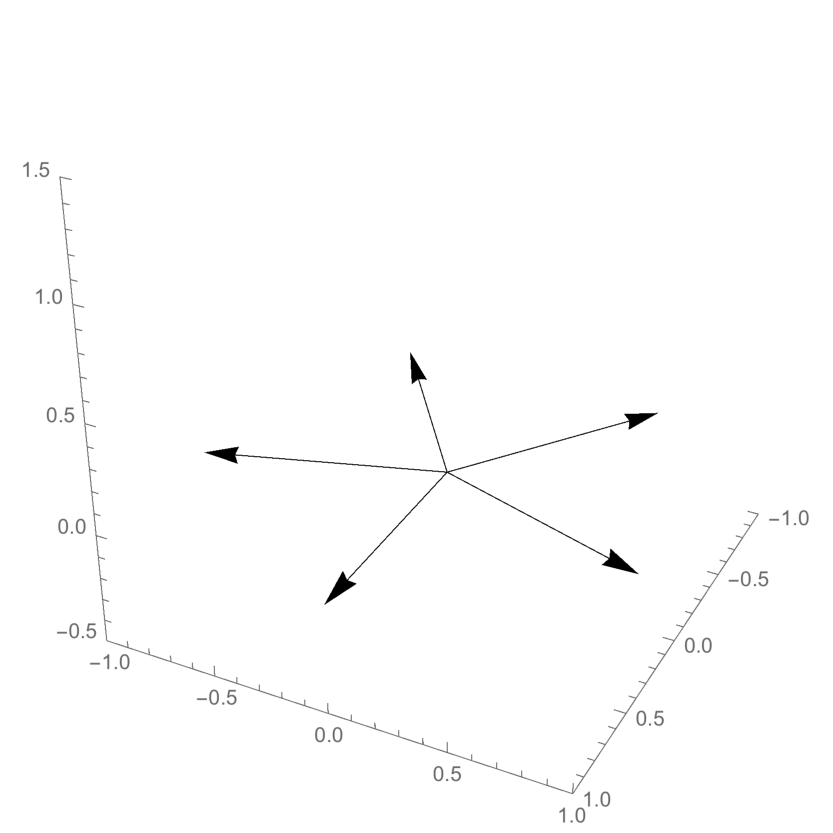
\includegraphics[width=.25\linewidth]{graphics/C5p=0.pdf}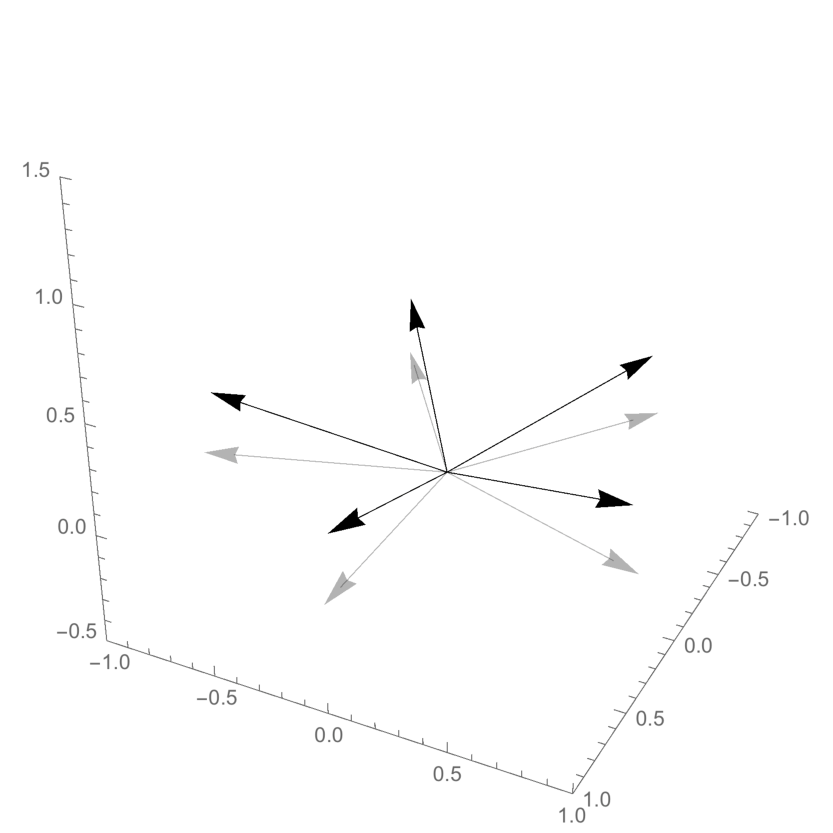
\includegraphics[width=.25\linewidth]{graphics/C5p=p3.pdf}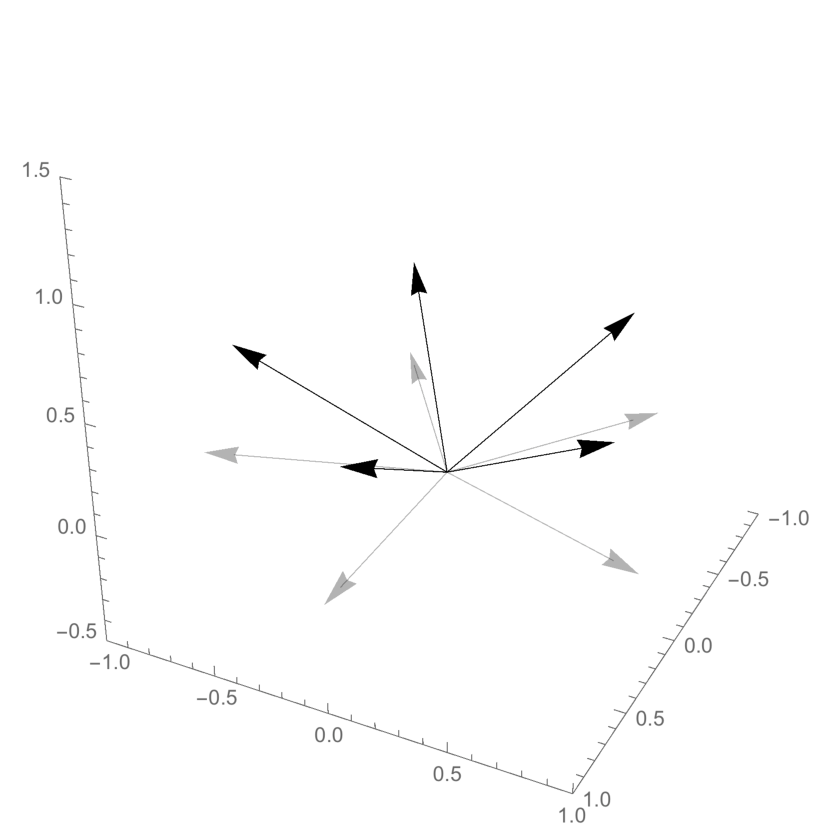
\includegraphics[width=.25\linewidth]{graphics/C5p=p6.pdf}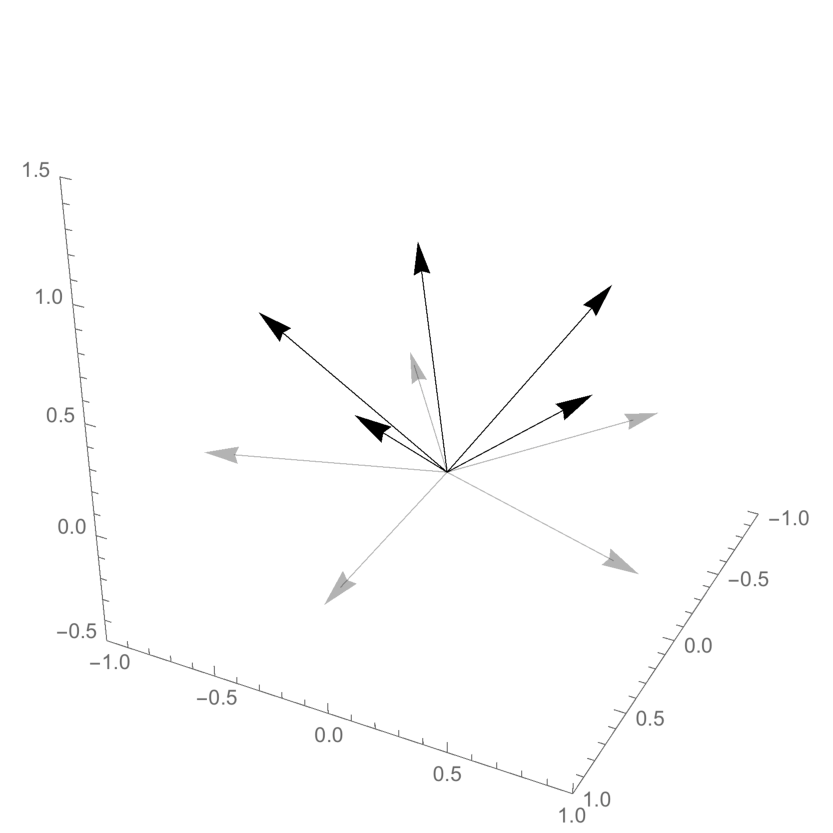
\includegraphics[width=.25\linewidth]{graphics/C5p=p0.pdf}
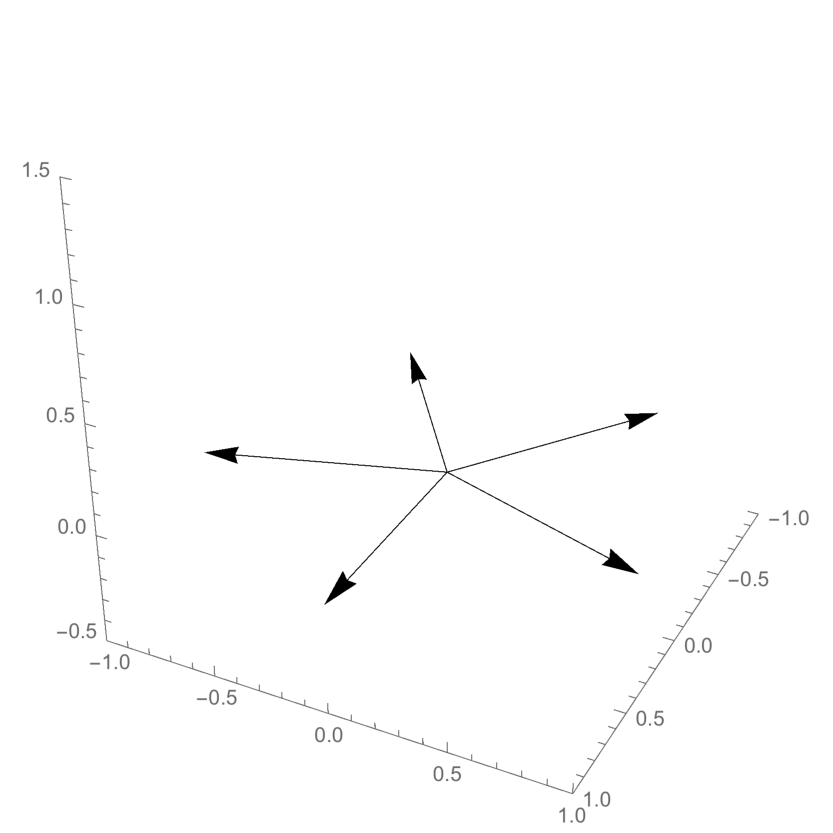
\includegraphics[width=.33\linewidth]{graphics/C5p=0.pdf}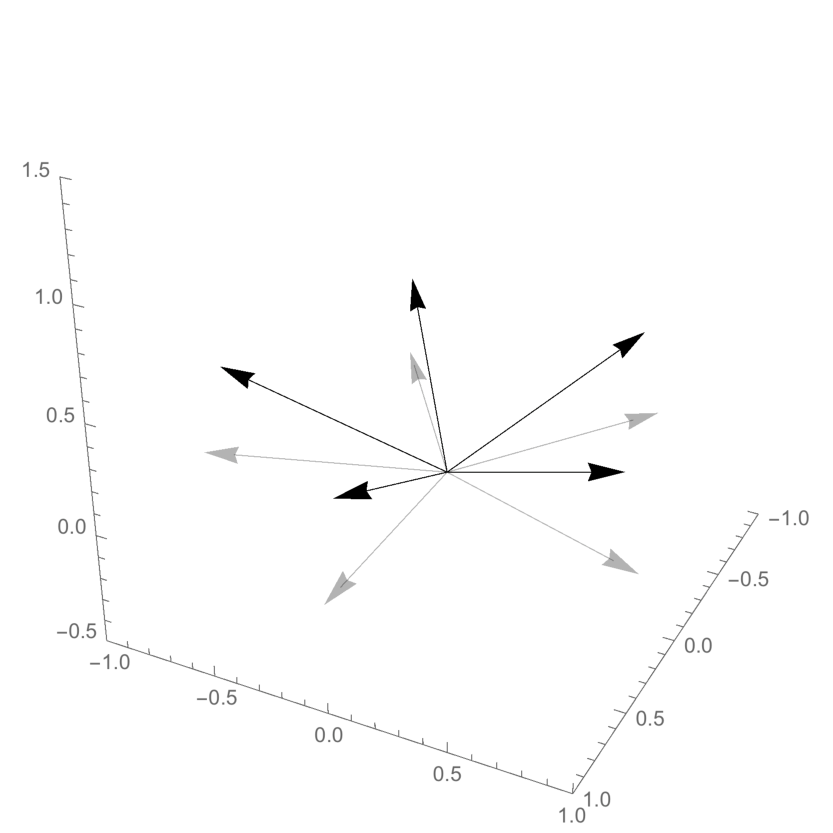
\includegraphics[width=.33\linewidth]{graphics/C5p=p45.pdf}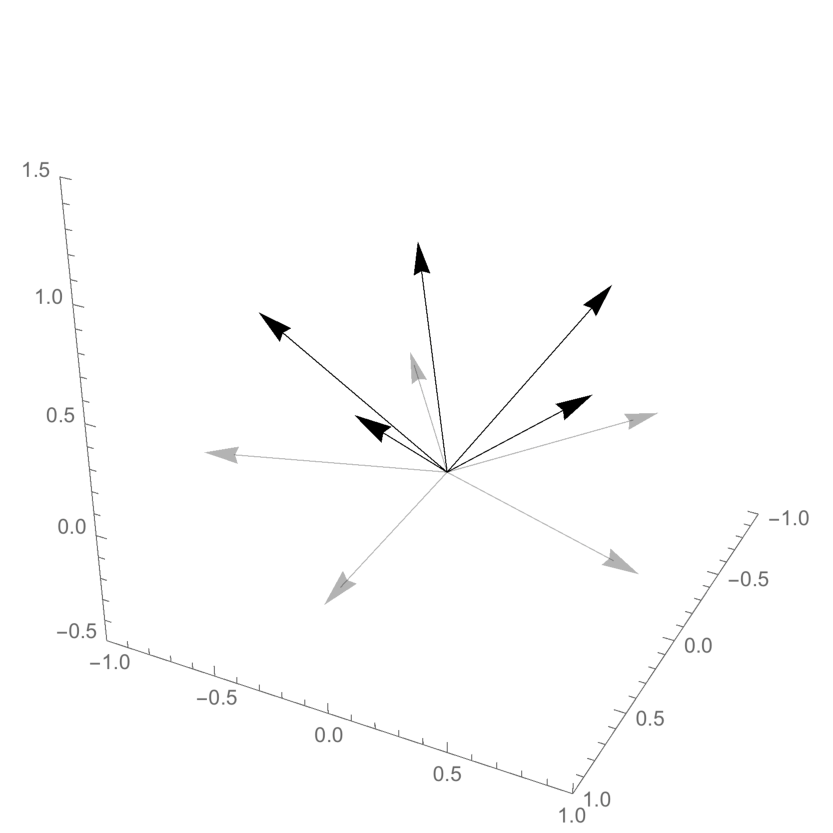
\includegraphics[width=.33\linewidth]{graphics/C5p=p0.pdf}
\caption{From left to right, the vectors $v_i$ with $p=0,0.45,\frac{1+\sqrt{5}}{4}\approx 0.89$. The intuition is that we are starting with our five vectors equally spaced on the unit circle. Then we ``close the umbrella'', increasing $p$, and pointing the vectors towards the $z$-axis, until each vector is orthogonal to the two vectors across from it.}
\end{figure*}

We have $(1,0,p) \perp (\cos \tfrac{4\pi}{5}, \sin \tfrac{4\pi}{5},p)$ if $-p^2 = \cos \tfrac{4\pi}{5}$. Then $p^2 = \frac{1+\sqrt{5}}{4}$. Now, we may check that at this value of $p$, each $v_i \perp v_{i+2},v_{i+3}$. That is, the $v_i$ form an orthonormal representation of $C_5$. Take $c = (0,0,1)$. Then $\braket{c,v_i} = \frac{p}{\sqrt{1+p^2}}$ for all $i$, and $\frac{1}{\big( \frac{p}{\sqrt{1+p^2}} \big)^2} = \dotsm = \sqrt{5}$.
\end{proof}
\begin{fullwidth}
\printbibliography[segment=\therefsegment,heading=subbibliography]
\end{fullwidth}


% \backmatter
\clearpage
\begin{fullwidth}
\printbibliography[heading=fullbib]

\printindex
\end{fullwidth}

\end{document}
